\documentclass[twoside,12pt,a4paper,openright]{memoir}
\maxsecnumdepth{subsubsection}			%Automatically number sections down to ``section'' level
\setsecnumdepth{subsubsection}
% \hyphenation{de-leer-snij-der}
\usepackage[utf8]{inputenc}			%Optimal font encoding for most latin languages
\usepackage[T1]{fontenc}
\usepackage{changepage}
\usepackage{pgfplots}
\usepackage{bm}
\usepackage{lipsum}
\usepackage[includehead, includefoot, top=2.35cm, bottom=2.35cm, outer=3.5cm, inner=3.5cm]{geometry}
% \usepackage[includehead, includefoot, top=4.8cm, bottom=4.8cm, outer=4.5cm, inner=4.5cm]{geometry} % l'option showframe est juste pour avoir le cadre défini par les bordures (pour voir ce qui dépasse dans les figures ou equations par ex.) 
\usepackage{bm}			%For bold symbols in math (command \bm)
\usepackage{lmodern}		%Font: latin modern (enhanced computer modern)


\usepackage{url}
\usepackage{threeparttable}

\usepackage{arydshln}

\usepackage[font=small]{caption}

\usepackage{color,calc,graphicx}
\newsubfloat{figure}% Allow subfloats in figure environment

\newcommand\red[1]{\textcolor{red}{#1}}
\newcommand\blue[1]{\textcolor{blue}{#1}}

\usepackage{geometry}
\newdimen\mywidth
\mywidth=0.91\textwidth
\newdimen\mywidthmesh
\mywidthmesh=0.80\textwidth
%\setlength{\belowcaptionskip}{-20pt}
\usepackage{siunitx} % for micro meters

% \usepackage{tikz}
% % \input{include/arrowsNew}
% \usetikzlibrary{shapes.misc}
% \tikzset{options/.code={\tikzset{#1}}} % just to compact the code
% \tikzset{cross/.style={cross out, draw=black, minimum size=2*(#1-\pgflinewidth), inner sep=0pt, outer sep=0pt},
% %default radius will be 1pt. 
% cross/.default={1pt}}

% \usetikzlibrary{decorations.pathmorphing, shadows}
% %\usetikzlibrary{arrows}
% \usetikzlibrary{shapes}

% \usetikzlibrary{positioning,calc,patterns} 
%\usetikzlibrary{external}
%\tikzexternalize[prefix=tikzext/] 

\usepackage{algorithm2e}


%For the glossary:
\usepackage{float}
% % Create new "listing" float
% \newfloat{listing}{tbhp}{lst}%[section]
% \floatname{listing}{Listing}

%Allow big floats:
\renewcommand{\topfraction}{.95}
\renewcommand{\bottomfraction}{.8}
\renewcommand{\textfraction}{.05}		%Allow minimal text with figures
\renewcommand{\floatpagefraction}{.85}		% require fuller float pages
	% N.B.: floatpagefraction MUST be less than topfraction !!
\renewcommand{\dbltopfraction}{.66}
\renewcommand{\dblfloatpagefraction}{.8}

% Command to set caption styles
\usepackage{etoolbox} 		%Needed for AtBeginEnvironment
\captionnamefont{\bfseries\small}
\captiontitlefont{\small}
\subcaptionlabelfont{\bfseries\small}
\subcaptionfont{\footnotesize}

\renewcommand{\figurename}{Fig.}

%For subappendices:
\usepackage{appendix}
\usepackage{chngcntr}
\AtBeginEnvironment{subappendices}{%
  \chapter*{Appendix}
  \addcontentsline{toc}{chapter}{Appendices}
  \counterwithin{figure}{section}
  \counterwithin{table}{section}
}
\AtEndEnvironment{subappendices}{%
  \counterwithout{figure}{section}
  \counterwithout{table}{section}
}

\renewcommand{\sfdefault}{lmss}
\usepackage{epstopdf}
\usepackage{fancybox}
\usepackage{booktabs}		% For \...rule lines in tables

%\usepackage[style=authoryear, 
%  sorting=nyt, 
%  sortcites=true, 
%  firstinits=true, 
%  uniquename=false, %2 lines to avoid initials in citations
%  uniquelist=false, %
%  doi=false, 
%  isbn=false, 
%  autopunct=true, 
%  maxcitenames=2,
%%   mincitenames=1,
%  maxbibnames = 1000,
%  uniquelist = false,		%Make 2008a, 2008b
%  backend=biber]{biblatex}

\usepackage{natbib}
\bibliographystyle{model2-names}


\usepackage{amsmath}
% \usepackage{amsfonts}
\usepackage{textcomp}						%For \textdegrees
\usepackage{verbatim}
\usepackage{amssymb}
% \usepackage{amsthm}
\usepackage{array}

% Enumerate with letters
\usepackage{enumerate}


\usepackage{empheq}

% \usepackage[round]{natbib}




\definecolor{red}{rgb}{1,0,0}
\definecolor{blue}{rgb}{0,0,0.8}
\definecolor{green}{rgb}{0,0.5,0}
%\newcommand{\emphc}[1]{}
\newcommand{\emphc}[1]{\emph{\textcolor{red}{#1}}}
\newcommand{\emphb}[1]{\emph{\textcolor{blue}{#1}}}
\newcommand{\modif}[1]{\textcolor{green}{#1}}







%
%%
%\usepackage{draftwatermark}
%\SetWatermarkText{DRAFT}
%\SetWatermarkScale{1}





%%%%%%%%%%% CONGO2D %%%%%%%%%

\usepackage{nicefrac}
\usepackage{xspace}
\usepackage{multirow}
% \newcommand{\gmsh}{{\textsc gmsh}\xspace}
% \newcommand{\rofi}{{\textsc rofi}\xspace}
\newcommand{\slim}{{\textsc slim}\xspace}
\newcommand{\UV}{\mathbf{U}}
\newcommand{\hycom}{\textsc{hycom} }
\newcommand{\ie}{\textit{i.e}} 
\newcommand{\eg}{\textit{e.g.}}

\DeclareSIUnit \year{y}
\DeclareSIUnit \cmetre{\metre\textsuperscript{\nicefrac{\num{-1}}{3}}}
\DeclareSIUnit \pmetre{\metre\textsuperscript{\num{0.85}}}
\DeclareSIUnit \centimetre{\centi\metre}


\newcommand{\clearemptydoublepage}{\newpage{\pagestyle{empty}\cleardoublepage}} 
\newcommand{\mychapter}[1]{\clearemptydoublepage \chapter{#1}}
\newcommand{\mychapterb}[2]{\clearemptydoublepage \chapter[#1]{#2}}
\newcommand{\mypart}[1]{\clearemptydoublepage \part{#1}}
\newcommand{\chapternonumber}[1]{\clearemptydoublepage \chapter*{#1 \markboth{#1}{}}\addcontentsline{toc}{chapter}{#1}}
\newcommand{\sectionnonumber}[1]{\section*{#1 \markright{#1}}\addcontentsline{toc}{section}{#1}}
\newcommand{\partnonumber}[1]{\clearemptydoublepage \part*{#1 \markboth{#1}{}}\addcontentsline{toc}{part}{#1}}

\newcommand{\bigcell}[2]{\begin{tabular}{@{}#1@{}}#2\end{tabular}} % For multiline cells inside tables

%Set headers at the top of pages
\nouppercaseheads
\makepagestyle{mystyle}
\makeevenhead{mystyle}{\thepage}{}{\itshape\leftmark}
\makeoddhead{mystyle}{}{}{\thepage}
\makeevenfoot{mystyle}{}{}{}
\makeoddfoot{mystyle}{}{}{}
\makepsmarks{mystyle}{%		Define what's in headers, see p12 of https://www.tug.org/pracjourn/2008-2/madsen/madsen.pdf
%   \createmark{section-heading-to-use}{define-for-left-or-right-side}{show-sec-nb?}{prefix-to-secNb}{suffix-to-secNb}
  \createmark{chapter}{left}{shownumber}{Chapter }{ - \ } 
}
% Nb: if I have appendices, will need to create new style so it isn't prefixed by Chapter

%   \makeheadrule{mystyle}{\textwidth}{\normalrulethickness}
% Extend the page numbers (& horiz line) into the margin
\makerunningwidth{mystyle}{1.\textwidth}
\makeheadposition{mystyle}{flushright}{flushleft}{flushright}{flushleft}
\makeheadrule{mystyle}{1.\textwidth}{\normalrulethickness}

\pagestyle{mystyle}

%Ref a footnote
\makeatletter
\newcommand\footnoteref[1]{\protected@xdef\@thefnmark{\ref{#1}}\@footnotemark}
\makeatother

%Set the style for the chapter headings
%\usepackage{fourier} %% I COMMENTED THIS!!
\DeclareSymbolFont{calletters}{OMS}{cmsy}{m}{n}
\DeclareSymbolFontAlphabet{\mathcal}{calletters}
%\usepackage[upright]{fourier}
\usepackage{soul}
%\definecolor{nicered}{rgb}{.647,.129,.149}
\definecolor{nicered}{rgb}{0.5,0.5,0.5}
\makeatletter
\newlength\dlf@normtxtw
\setlength\dlf@normtxtw{\textwidth}
\def\myhelvetfont{\def\sfdefault{mdput}}
\newsavebox{\feline@chapter}
\newcommand\feline@chapter@marker[1][4cm]{%
  \sbox\feline@chapter{%
     \resizebox{!}{#1}{\fboxsep=1pt%
       \colorbox{nicered}{\color{white}\bfseries\sffamily\thechapter}%
     }}%
  \rotatebox{90}{%
     \resizebox{%
       \heightof{\usebox{\feline@chapter}}+\depthof{\usebox{\feline@chapter}}}%
     {!}{\scshape\so\@chapapp}}\quad%
  \raisebox{\depthof{\usebox{\feline@chapter}}}{\usebox{\feline@chapter}}%
}
\newcommand\feline@chm[1][4cm]{%
  \sbox\feline@chapter{\feline@chapter@marker[#1]}%
  \makebox[0pt][l]{% aka \rlap
     \makebox[1cm][r]{\usebox\feline@chapter}%
  }}
\makechapterstyle{daleif1}{
  \renewcommand\chapnamefont{\normalfont\Large\scshape\raggedleft\so}
  \renewcommand\chaptitlefont{\normalfont\huge\bfseries\scshape}%\color{nicered}}
  \renewcommand\chapternamenum{}
  \renewcommand\printchaptername{}
  \renewcommand\printchapternum{\null\hfill\feline@chm[3cm]\hspace*{1cm}\par}
  \renewcommand\afterchapternum{\par\vskip\midchapskip}
  \renewcommand\printchaptertitle[1]{\chaptitlefont\raggedleft ##1\par}
}
\makeatother
\chapterstyle{daleif1}



%\newenvironment{abstract}{
%\begin{center}
%\begin{minipage}{0.85\textwidth}
%\begin{center}\textbf{Abstract}\end{center}
%\small
%}{
%\end{minipage}
%\end{center}
%}


% \newenvironment{paperresume}{%
% %\small
% \noindent\rule{\textwidth}{0.2mm}%\\[5mm]
%   \list{}{%
%     \leftmargin 0.025\textwidth
%     \rightmargin \leftmargin
%   }%
%   \item[]
% }
% {\endlist
% \noindent\rule{\textwidth}{0.2mm}%\\[5mm]
% }
% \newcommand {\myrule}{ \noindent\rule{\textwidth}{0.2mm}}

% \newcommand{\getbibliographyitem}[1]{
% \immediate\write18{./singleref #1}
% \vspace*{-0.5em}
% \renewcommand{\prebackcite}{}
% \renewcommand{\postbackcite}{}
% \input{tmp.bbl}
% \renewcommand{\prebackcite}{Cited on p.~}
% \renewcommand{\postbackcite}{.}
% }


%% shortcuts for formulae
% \newcommand{\pd}[2]{\frac{\partial #1}{\partial #2}}
% \newcommand{\diff}[2]{\frac{\mathrm{d} #1}{\mathrm{d} #2}}
% \newcommand{\bnabla}{\bm{\nabla}}
% \newcommand{\bu}{\bm{u}}
% \newcommand{\bbu}{\bm{\bar{u}}}%
% \newcommand{\bub}{\bm{u}_b}%{\underaccent{\bar}{u}_b}%
% \newcommand{\bw}{\bm{w}}%{\underaccent{\bar}{W}}%{\bm{W}}

% \newcommand{\vint}[2][K]{\Big\langle #2  \Big\rangle_{\!\!#1}}
% \newcommand{\vintsmall}[2][K]{\big\langle #2  \big\rangle_{\!#1}}
% \newcommand{\sint}[2][e]{\Big\langle\!\!\Big\langle #2 \Big\rangle\!\!\Big\rangle_{\!\!#1}}
% \newcommand{\sintsmall}[2][e]{\big\langle\!\big\langle #2 \big\rangle\!\big\rangle_{\!\!#1}}
% \newcommand{\lint}[2][e]{\Big\langle\!\!\Big\langle\!\!\Big\langle #2 \Big\rangle\!\!\Big\rangle\!\!\Big\rangle_{\!\!#1}}
% \newcommand{\mean}[1]{\{#1\}}
% \newcommand{\jump}[1]{[#1]}
% \newcommand{\maxi}[1]{\lceil#1\rceil}
% \newcommand{\roe}[1]{#1_\text{Roe}}
% \newcommand{\bpsi}{\bm{\psi}}
% \newcommand{\bn}{\bm{n}}
% \newcommand{\bt}{\bm{t}}
% \newcommand{\bq}{\bm{q}}
% \newcommand{\bx}{\bm{x}}

% \newcommand{\bbarU}{\bar{\bm{U}}}
% \newcommand{\btau}{\bm{\tau}}
% \newcommand{\br}{\bm{r}}

% \newcommand{\BE}{ \begin{enumerate}}
% \newcommand{\EE}{ \end{enumerate}}
% \newcommand{\BI}{ \begin{itemize}}
% \newcommand{\EI}{ \end{itemize}}
% \newcommand{\BEQ}{ \begin{equation}}
% \newcommand{\EEQ}{ \end{equation}}
% \newcommand{\BDM}{ \begin{displaymath}}
% \newcommand{\EDM}{ \end{displaymath}}
% \newcommand{\ds}{\displaystyle}
% \newcommand{\ud}{\textrm{ d}}
% \newcommand{\BTc}{ \begin{tabular}{c}}
% \newcommand{\BTcc}{ \begin{tabular}{cc}}
% \newcommand{\BTl}{ \begin{tabular}{l}}
% \newcommand{\BTr}{ \begin{tabular}{r}}
% \newcommand{\ET}{ \end{tabular}}
% \newcommand{\BS}{ \begin{small}}
% \newcommand{\ES}{ \end{small}}
% \newcommand{\BEQQ}{ \begin{equation*}}
% \newcommand{\EEQQ}{ \end{equation*}}


\definecolor{darkgreen}{rgb}{0.0,.6,0.0}
\newcommand{\GG}[1]{}
\pgfplotsset{compat=1.15}
\usepackage[pdftex,linktocpage]{hyperref}		%For hyperlinks within doc, and setting doc info
\hypersetup{pdftitle={How modeling tools can inform coral reef management in Florida}}
\hypersetup{pdfauthor={Thomas DOBBELAERE}}
\hypersetup{pdfsubject={How modeling tools can inform coral reef management in Florida}}
\hypersetup{pdfkeywords={Biophysical modeling, Florida Coral Reef, SCTLD, SLIM}}
% % Comment out next hypersetup section for print version:
%\hypersetup{
%  colorlinks=true,
%  citecolor=blue,
%  linkcolor=blue,
%  urlcolor=blue
%}
\hypersetup{
  colorlinks=true,
  citecolor=black,
  linkcolor=black,
  urlcolor=black
}
% % % %   citebordercolor={0.8 0.8 0.8},
% % % %   filebordercolor={0.8 0.8 0.8},
% % % %   linkbordercolor={0.8 0.8 0.8},
% % % %   menubordercolor={0.8 0.8 0.8},
% % % %   urlbordercolor={0.8 0.8 0.8},
% % % %   runbordercolor={0.8 0.8 0.8} 


% \usepackage{cmbright}				%TODO: this doesn't compile when I add it *** Font: Computer modern bright
% \usepackage{sfmath}				%Display all maths with sans serif font
\renewcommand\familydefault{\sfdefault} 

\begin{document}
\frontmatter
  \thispagestyle{empty}
\begin{minipage}[b]{0.3\textwidth}
\hspace*{-0.8cm}
\includegraphics[width=5.5cm]{./figures/logo_ucl.jpg}\vspace{0.85cm}
%\hspace*{3.4cm}
\includegraphics[width=4.5cm]{./figures/orb.png}\vspace*{.1cm}
\end{minipage}
\begin{minipage}[b]{0.69\textwidth}

\begin{center}
\hspace*{0.5cm}Université Catholique de Louvain\\
\hspace*{0.5cm}\'Ecole Polytechnique de Louvain\\
\hspace*{0.5cm} Earth and Life Institute\\
\end{center}
\end{minipage}


\vspace*{1.2cm}
\hspace{-0.8cm}
\begin{minipage}{1.02\linewidth}
\centering
\LARGE\bfseries How modeling tools can inform coral reef management in the Florida Reef Tract
\end{minipage}


\vspace*{0.5cm}
\hspace{-0.5cm}\begin{minipage}{\textwidth}
\centering
\rule{50pt}{.5pt}\\[1.2ex]
Doctoral dissertation presented by \\ [2.ex]
{\Large Thomas Dobbelaere\\ [2.ex]
}
in partial fulfillment of the requirements for the degree of\\ [2.ex]
\Large Docteur en Sciences de l'ingénieur

\rule{50pt}{.5pt}\\
\end{minipage}

\vspace*{1.5cm}
\begin{minipage}{\textwidth}
\begin{center}

\large Thesis committee:\\

\vspace*{0.5cm}
\footnotesize{
\hspace{-1.2cm}
\begin{tabular}{ll}
Prof. Emmanuel Hanert (Supervisor) & Université Catholique de Louvain \\
Prof. Eric Deleersnijder           & Université Catholique de Louvain \\
Dr. Jonathan Lambrechts            & Université Catholique de Louvain\\
???                                & ??? \\
???                                & ??? \\ 
\end{tabular}
}
\end{center}
\end{minipage}

\vspace*{.5cm}
\vspace*{\stretch{1}}
\begin{minipage}{\textwidth}
\centering
\large Louvain-la-Neuve, March 2022
\end{minipage}

  \clearemptydoublepage
  
\chapter*{Abstract}
%\phantom{Abstract}

Coral populations have declined dramatically worldwide under the combined effects of climate change and local anthropogenic stressors. In addition to ocean warming and acidification, threats to coral reefs in the Caribbean include frequent and virulent disease outbreaks, and intensifying hurricanes. In particular, Florida's Coral Reef (FCR) is currently facing a multi-year outbreak of the stony coral tissue loss disease (SCTLD). First observed in 2014 during the monitoring of the PortMiami Deep Dredge Project (PMDDP), the disease has now spread through the entire FCR and has been reported in numerous territories of the Caribbean. However, the propagation of the disease through FCR seemed to slow down when it reached its southwestern end, between the Marquesas and the Dry Tortugas (DRTO). Although the causative agent of the disease remains unknown, studies showed that its transmission was likely waterborne and that sediments could act as SCTLD vectors. The hydrodynamics should therefore be highly explanatory of its spread. Furthermore, Florida is a prime landfall target for hurricanes during the reproduction period of corals. In addition to causing wholesale destruction of the reefs, hurricanes might thus also impact larval dispersal through wind-wave-induced currents. Here, we use the high resolution coastal ocean model SLIM to capture transport processes in the FCR, and study the impact of SCTLD and hurricanes to coral reefs. First, a coupled epidemio-hydrodynamic model is developed to reproduce and understand the observed spread of SCTLD in Florida. A sediment transport model is then used to evaluate the impact of the PMDDP on the observed onset of the disease in 2014. Finally, a coupled wave-current model is implemented to study the impact of Hurricane Irma (2017) on transport processes over reefs in the Florida Keys. Assuming the dispersal of disease agents within neutrally buoyant material, our model successfully reproduced the observed spread of SCTLD through the FCR and linked its apparent stalling before reaching the DRTO to eddy activity in the Loop Current/Florida Current system. Furthermore, the results of our sediment transport model suggest that the PMDDP might have triggered the onset of the disease. Finally, our coupled wave-current model showed the important impact of wave-induced currents on transport processes over reefs during hurricanes. This thesis highlights the potential of models informed by and confronted against field knowledge as powerful tools to inform the management of complex marine ecosystems such as the FCR.

%The population of corals throughout the world has declined dramatically and many coral species are now listed as threatened Avoiding global warming being no longer an option, reef managers now focus on damage control and restoration strategies. The Florida Reef Tract, currently facing an unprecedented coral disease outbreak and where healthy corals grown in nurseries are replanted on damaged reefs, is a good application case of such reef management strategies. In order to maximize the efficiency of these efforts, a good knowledge of exchanges of infectious materials and larvae between reefs is required. However, connectivity patterns between reefs remain mostly unknown. To address this issue, we will use the high-resolution ocean model SLIM to simulate connectivity patterns between reefs and then identify reefs with the highest restoration potential as well the ones that are most at risk of being infected by the outbreak. 


%The dispersal of coral larvae away from their natal habitats is an important process for coral reef ecosystems, but remains poorly understood and hard to gauge. This thesis presents a spatially explicit numerical modelling approach to simulate larval dispersal in Australia's Great Barrier Reef (GBR), and in doing so to estimate connectivity between the thousands of reefs that comprise it. A high resolution, finite element ocean model, SLIM, is used to build a biophysical model of larval dispersal capable of estimating larval exchange between reefs in large sections of the the GBR. Tools from network science are employed to investigate the community structure of the GBR's connectivity network, and these tools are used to reveal the presence of clusters of highly inter-connected reefs. Subsequently, the model is used to estimate the extent of connectivity between reefs of different morphologies and depths in the GBR. Finally, the possible impacts of climate change on connectivity in the GBR are assessed, and estimates are made of the likely changes to coral larval dispersal patterns over the coming century.

%Titan, Saturn’s largest moon, is a unique object in the Solar system as much as it has a substantial atmosphere, a surface with a complex interplay of geological processes and an outer ice shell overlyinga subsurface ocean. The climate on this icy satellite boasts a multi-phase hydrological cycle where methane plays a role similar to that of water on Earth. Surface lakes and seas filled with liquid methane and ethane are found in the polar regions. The subsurface ocean, on the other hand, is filled with liquid water. This liquid layer lying beneath Titan’s surface allows for the large surface deformation observed.

%The first objective of this thesis was to adapt an Earth-based geophysical and environmental model, SLIM (www.climate.be/slim), to Titan’s specific conditions in order to study the tidal motion in the surface lakes and seas. The modified model was applied to the largest lake in the southern hemisphere, Ontario Lacus, and the two largest seas, Kraken and Ligeia Maria, which are located in the northern hemisphere. The predicted surface elevation and velocity fields are part of the data needed to develop an exploration mission focusing on the surface lakes and seas of Titan. The normal modes of Ontario Lacus were also numerically studied. While resonantly forced modes could generate significant liquid motion, the natural periods are much shorter than the period of the astronomical forcings. Therefore, only atmospheric forcings could resonantly force the normal modes. Strong wind conditions corresponding to a stormy event are required to generate a surface elevation resulting in significant shoreline variations.

%Then, the model was used to study the tides of Titan’s global subsurface ocean. To this end, the shallow water equations and the 3D hydrostatic equations under the Boussinesq approximation were modified in order to take into account the ice shell lying at the top of the ocean. The method was adapted to solve the equations on a sphere. The effects of the shell are represented by adding a surface friction and a surface pressure term. The shell decreases the ocean surface elevation and slows down the flow without modifying significantly the global patterns of these fields. The magnitude of these variations depends on the mechanical behaviour of the ice shell. Surface and bottom heat fluxes play a significant role in the liquid motion of the ocean. The interactions between the tidal motion and the thermally driven flow resulting from the surface heat flux were studied by means of the 3D version of SLIM. The surface heat flux significantly impacts the velocity field, both in terms of magnitude and orientation while the influence on the ocean’s surface elevation is small. These results could be useful for astrobiologists paying attention to the ocean habitability and to validate hypotheses about Titan’s internal structure.
  %\clearemptydoublepage
   \phantom{thanks}
%\textit{Remerciements à }
\chapter*{Remerciements}

Mes premiers remerciements vont à mon promoteur, le professeur Emmanuel Hanert, le grand chef qui m'a guidé et accompagné tout au long de cette thèse. D'une énergie et surtout d'un optimisme à toute épreuve (si toutes ses prédictions s'étaient avérées exactes, cette thèse aurait été finie en 1 ans), il m’a poussé et soutenu durant les quatre dernières années. En outre, il a toujours réussi à accomplir le miracle de dégager du temps dans son agenda bien chargé pour me conseiller ou relire et commenter mon travail avec minutie. Je tiens également à remercier tous les membres de mon jury pour le temps qu'ils ont accordé à la lecture de ce manuscrit ainsi que pour leurs judicieux conseils et suggestions lors de la défense privée. 

Je remercie également le groupe de vie ENGE, qui m'a accueilli durant les bientôt quatre années de cette thèse. Ce groupe hétéroclite m'a fourni un cadre de travail convivial, agrémenté de pauses café, de verres à la quinzaine et de soupers de Noël endiablés. Ce fut un plaisir de les avoir comme collègues et je ne pourrai désormais plus manger de burrito sans penser à eux. Parmi eux, je tiens particulièrement à remercier mon fidèle voisin de bureau et excellent camarade de conférence, Antoine Saint-Amand. Il m'a guidé et accompagné au cours de mon épopée dans la jungle de la thèse et a été une source intarissable de bonnes histoires et anecdotes. De plus, son engagement à la ville comme à l’université ainsi que son dévouement pour ses étudiants ont été une source d’inspiration. Il me reste à remercier l’autre mouscronnois du bureau, Valentin Vallaeys, pour son humour et sa propension à inonder ses collègues de sucreries. En outre, son don inégalé pour poser les bonnes questions m'a plus d'une fois permis d’entrevoir une issue à un problème apparemment insoluble l’instant d’avant.

Je tiens également à remercier tous les autres membres de la team SLIM. Ce fut un plaisir de travailler avec eux au développement de ce modèle. Parmi eux, je tiens à remercier spécialement Jonathan Lambrechts, qui rend l’impossible possible en 3 coups de clavier. Malgré les nombreuses sollicitations qu’il reçoit, il s'est toujours rendu disponible pour me débugger et cette thèse aurait été techniquement impossible sans lui. À ce propos, un échange téléphonique particulièrement éclairant me revient en mémoire: “Salut Jon, est-ce que tu as un peu de temps pour m’aider ? Non, mais dis toujours.”... 5 minutes plus tard, le problème était réglé.

I would also like to thank the team of collaborators and co-authors that started in 2019 with Lew Gramer, later joined by Erinn Muller and Dan Holstein, and has been growing ever since. It has been a real pleasure to work with them on all these exciting projects. I would like to extend my thanks to Pr Sam Purkis and Ceci Lopez-Gamundi. Although unraveling the mysteries of the Great Bahama Bank was not directly linked to the subject of this thesis, it has been a pleasure to join them in this geological quest. Et tant qu’on est à Miami, je remercie également Matthieu le Hénaff, qui garde un œil sur nos projets floridiens en coulisse. Ses conseils avisés ainsi que les personnes avec lesquelles il nous a mis en contact ont été d’un grand secours.

Il convient également de remercier ceux qui n'ont probablement pas contribué à me rendre plus productif mais ont assurément rendu ces années de thèse beaucoup plus amusantes. Tout d'abord, il me faut remercier les 36 "voix" du kot Carrefour. Cette grande famille m'a permis de rencontrer des gens d'origines et de cultures variées tout en me fournissant un lieu de vie calme (à l’exception de quelques folies) pour mener à bien cette thèse. Les prochains remerciements sont pour l’équipe de l'Oenokot, qui réussit à convaincre tout le monde (même mes anciens étudiants) que je suis un étudiant en BAC2 de droit. Des remerciements tout particuliers s'imposent pour le dénominateur commun à ces deux bandes de joyeux lurons, Redge, qui me supporte depuis presque 5 ans malgré des premiers contacts difficiles au kot Erasmus. Enfin, je remercie la Revue des Ingénieurs, qui offre un auditoire à mes blagues depuis 9 ans et qui, jusque dans les derniers jours de la rédaction de cette thèse, m’a fourni quelques bons prétextes à la procrastination.

\vspace{3em}

Ce travail a été financé par le Fonds de la Recherche Scientifique - FNRS au moyen d’une bourse FRIA.

  \clearemptydoublepage
  \tableofcontents
  \clearemptydoublepage
  % 
\chapter*{List of acronyms and abbreviations}

\begingroup
\setlength{\tabcolsep}{20pt}
\renewcommand{\arraystretch}{1.3}
\begin{tabular}{ll}
	\textbf{ADCP}   & Acoustic Doppler Current Profiler\\
	\textbf{DRTO}   & Dry Tortugas \\
	\textbf{ECMWF}  & European Centre for Medium-Range Weather Forecast \\
	\textbf{D55}    & Dredge 55 clamshell \\
	\textbf{FC}     & Florida Current \\
	\textbf{FCR}    & Florida's Coral Reef \\
	\textbf{FRT}    & Florida Reef Tract  \\
	\textbf{GoM}    & Gulf of Mexico \\
	\textbf{HURDAT} & HURricane DATabases \\
	\textbf{HYCOM}  & HYbrid Coordinate Ocean Model \\
	\textbf{LC}     & Loop Current \\
	\textbf{NOAA}   & National Oceanographic and Atmospheric Administration \\
	\textbf{ODMDS}	& Ocean Dredge Material Disposal Site \\
	\textbf{PoM}    & Port of Miami \\
	\textbf{PMDDP}  & PortMiami Deep Dredge Project \\
	\textbf{RS}     & Radiation stress \\
	\textbf{SB}     & Spider Barge \\
	\textbf{SCTLD}  & Stony coral tissue loss disease \\
	\textbf{SLIM}   & Second-generation Louvain-la-Neuve Ice-ocean Model\\
	\textbf{SWAN}   & Simulating WAves Nearshore \\
	\textbf{TI}     & Terrapin Island hopper \\
	\textbf{TX}     & Texas cutterhead \\
	\textbf{WWTP}	& Wastewater Treatment Plant \\
	\textbf{WFS}    & West Florida Shelf
\end{tabular}
\endgroup
  % \clearemptydoublepage
  \mainmatter 
%%%%
\mychapter{Introduction} \label{chap:intro}
 \section{Coral reefs: a rich but threatened ecosystem}

Coral reefs are among the most productive and biologically diverse ecosystems on Earth \citep{connell1978diversity, moberg1999ecological}. They supply food, income and coastal protection to vast numbers of people (Fig. \ref{intro:corals}). While they account for less than 0.5\% of the ocean floor \citep{spalding1997new}, they are home for almost a third of the marine biodiversity \citep{moberg1999ecological}. Reef-related fisheries account to up to 40\% of the total marine
fish landed value of some regions \citep{teh2013global} and hundreds of millions of people depend on coral reefs for their livelihood or part of their protein intake \citep{salvat1992coral,hoegh2019people}. Through calcification, corals are the backbone of a complex three-dimensional habitat that serves as spawning, breeding and feeding area for many species \citep{moberg1999ecological}. This complex reef framework  dissipates most of incoming waves energy, protects shorelines from storms and floods, and prevents coastal erosion \citep{ferrario2014effectiveness,elliff2017coral}. Additionally, wave dissipation creates lagoon and sedimentary environment, providing favorable conditions for the growth of seagrass and mangrove ecosystems \citep{moberg1999ecological}.

\begin{figure}
    \centering
    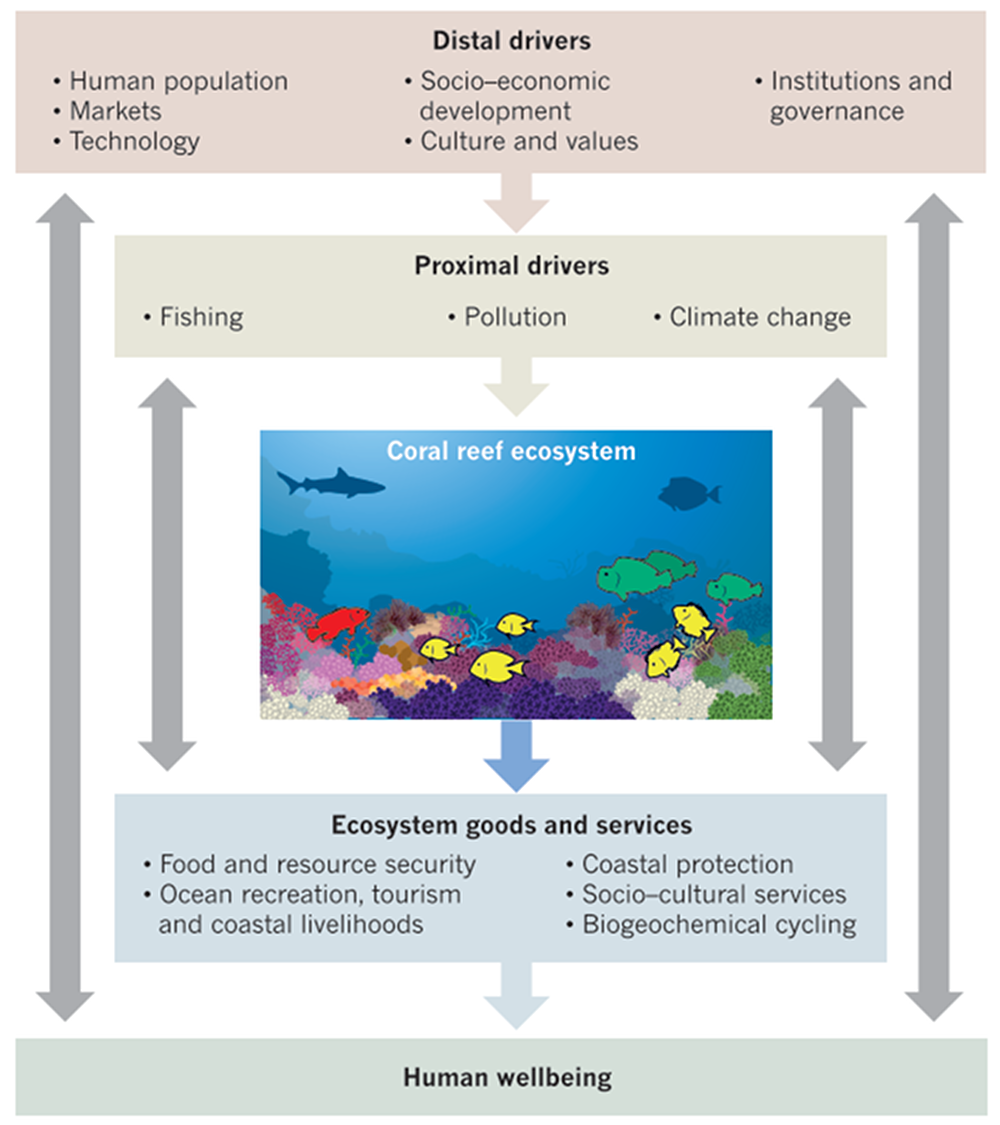
\includegraphics[width=.8\textwidth]{chapters/intro/figures/anthropocene.png}
    \caption{Goods and services of coral reefs and their linkage with human activities. Source: \cite{hughes2017coral}}
    \label{intro:corals}
\end{figure}

The calcifying process of reef building corals heavily depends on their symbiosis with the microalgae zooxanthellae. These unicellular symbionts convert sunlight and carbon dioxide into organic carbon and oxygen, providing the corals with most of the energy needed to meet their metabolic demands \citep{muscatine1977reef}. However, adverse environmental conditions such as elevated sea surface temperature can cause damage to the mechanisms maintaining this association, resulting in the expulsion of the endosymbionts \citep{hoegh2007coral}. This process, called bleaching, causes the coral to loose their pigmentation and reveals their underlying white skeleton \citep{baker2008climate}. Bleached corals are physiologically and nutritionally compromised, and prolonged bleaching over several months leads to high coral mortality \citep{hughes2018spatial}. Decline in coral health and cover pushes the reef ecosystem to a macroalgal-dominated state \citep{hughes2003climate,mumby2007thresholds}. Once a "tipping point" is exceeded, returning to a coral-dominated state becomes difficult \citep{mumby2007thresholds,graham2015predicting}.

Despite their importance, coral reefs have experienced a massive system-wide decline: it is estimated  that 50\% have already been severely damaged, and almost all could be lost under a 1.5$^\circ$C warming \citep{hoegh2019people,dixon2022future}. This global decline in live coral cover \citep{gardner2003long,pandolfi2003global,pandolfi2011projecting,bruno2007regional,perry2013caribbean,dove2020ocean} (Fig. \ref{intro:cover}) is caused by both global and local anthropogenic stressors. The main global stressors are climate change induced ocean warming and acidification. Ocean warming causes recurrent mass bleaching events at an increasing frequency \citep{connell199730, hughes2018spatial}. Furthermore, thermal stress can increase the susceptibility of corals to disease, leading to an increase in the incidence of coral disease outbreaks \citep{harvell2002climate,bruno2007thermal,muller2012caribbean}. Moreover, the increase of the concentration of atmospheric carbon dioxyde causes a decrease of the pH and carbonate concentration of seawater. As a result, coral calcification and growth decrease, which inhibits their capacity to build structurally complex habitats \citep{hoegh2007coral}. Local stressors are numerous and include pollution \citep{loya1980effects}, coastal development and the associated sediment and wastewater fluxes \citep{erftemeijer2012environmental, cunning2019extensive}, nutrient run-off \citep{hughes2003climate,sheppard2017biology}, and overfishing of herbivorous species controlling algae growth \citep{jackson2001historical}.

\begin{figure}
    \centering
    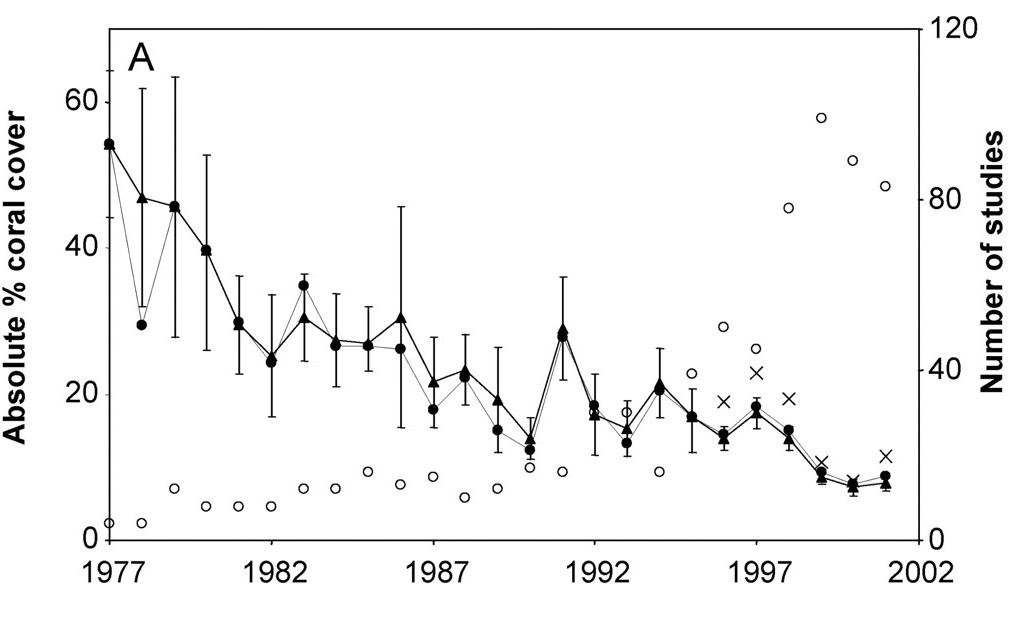
\includegraphics[width=.9\textwidth]{chapters/intro/figures/cover.jpeg}
    \caption{Evolution of the absolute coral cover in the Caribbean. Source: \cite{gardner2003long}}
    \label{intro:cover}
\end{figure}

Due to the combined damages from of all these stressors, it is almost impossible to return reefs to their past configurations \citep{hughes2017coral}. Instead, the challenge is now to maintain the biological functions of coral reefs through quickly changing environmental conditions. This will require to rapidly address greenhouse gas emissions, as well as local actions to boost the capacity of coral reef ecosystems to survive climate change \citep{hughes2003climate,knowlton2008shifting,graham2015predicting}. The aim of the present dissertation was therefore to use modeling tools to better understand the drivers of coral demise and hence inform such local actions to support ecosystem management in Florida, the third largest barrier reef of the world.

\section{Identifying the threats to coral survival in Florida}

The Florida Reef Tract (FRT) spans over approximately 577 km from the Dry Tortugas (DRTO) west of the Florida Keys to the St. Lucie Inlet in Martin County, constituting the third largest barrier reef in the world \citep{finkl2008shelf} (Fig. \ref{intro:frt}). These reefs harbor a rich Caribbean fauna, including more than 40 species of stony corals \citep{banks2008reef,jackson2014status}. The northern half-section of the FRT consists of relic, Holocene framework reefs and indurated sand ridges, divided into three shore-parallel reefs (inner, middle, outer) separated by sandy plains. Benthic cover is generally denser on the middle and outer reefs while the inner reef harbors some large patches of dense \textit{Acropora cervicornis}. The dominant reef builder is the bouldering \textit{Montastraea cavernosa} but living hard coral cover is fairly low (below 3\%)\citep{banks2008reef,walton2018impacts}. The southern half-section is a chain of limestone islands (the Keys) that extend from the southern tip of the Florida mainland southwest to the DRTO on the the boundary of the West Florida Shelf (WFS). The Upper Keys are remnants of ancient coral reefs and the Lower Keys are sand bars \citep{hoffmeister1968geology}. The DRTO are made of small circular reef banks whose coral populations are among the most preserved of the continental United States \citep{hine2008coral, kourafalou2018physical}. Moreover, they are believed to be important sources of recruitment for coral-reef fishes in the Florida Keys \citep{domeier2004potential}. 

\begin{figure}
    \centering
    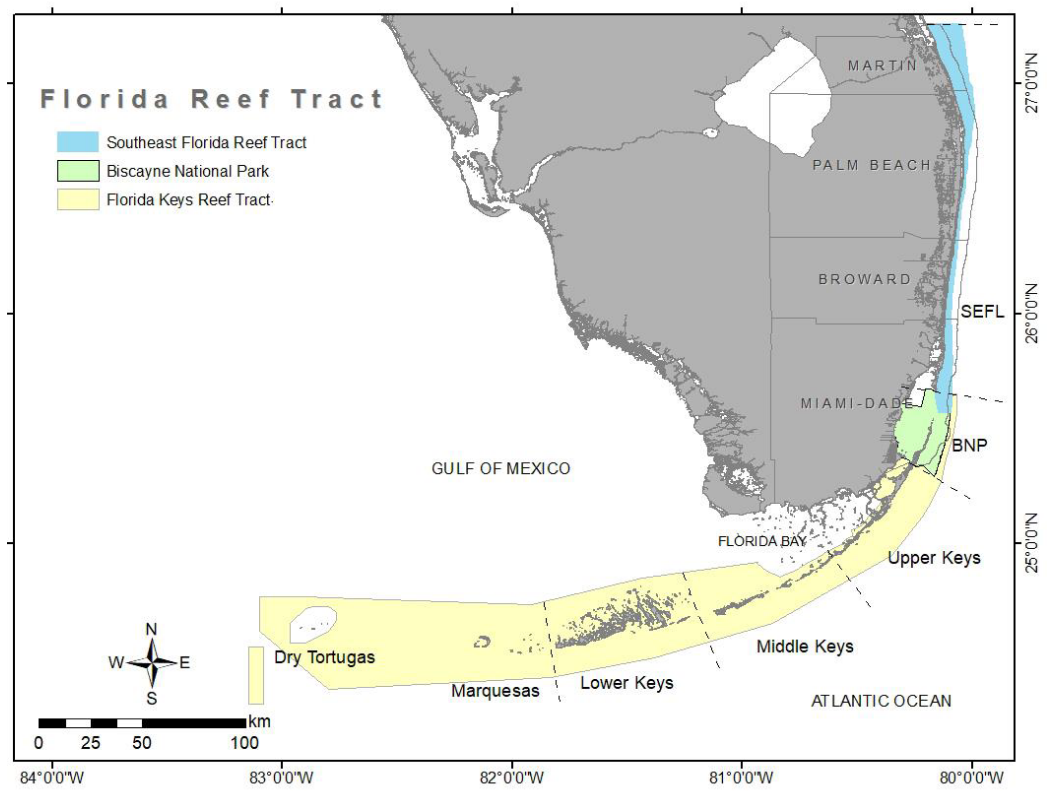
\includegraphics[width=\textwidth]{chapters/intro/figures/frt.png}
    \caption{Map of Florida Reef Tract with major features and divisions. Source: \cite{kupfner2019untapped}}
    \label{intro:frt}
\end{figure}

Florida's Coral Reef (FCR) is of considerable importance to the economy of the state. \cite{johns2003socio} estimated the contribution of recreational users of natural and artificial reefs over the period June 2000 to May 2001 to have been US\$2.3 billions in sales and US\$1.1 billion in income. Moreover, recreational use of the reefs was evaluated to bring 36,500 full and part-time jobs. Focusing on natural reefs only, \cite{brander2013total} estimated the total coral reef values Florida to be US\$174 millions. However, this value might be strongly underestimated as non-use and indirect use values, such as support for coastal fisheries \citep{ault2006building} and coastal protection \citep{ferrario2014effectiveness} were not taken into account.

Nevertheless, FCR has been heavily impacted by the human activities of the major metropolitan area of greater Miami. These impacts include densely populated coastlines, large numbers of visitors, polluted terrestrial run-off and overfishing \citep{jackson2014status}. For example, dredging operations during the PortMiami Deep Dredge Project (PMDDP) was reported to have caused the death of $>$560,000 corals \citep{cunning2019extensive}. Florida's coral reefs have therefore declined significantly over the past decades due to anthropogenic stressors and numerous disease outbreaks \citep{gardner2003long, jackson2014status}. Populations of previously dominant reef-building acroporids almost totally disappeared throughout the Caribbean and Florida \citep{aronson2001white}, and coral cover dropped from 40 to 60\% in 1975 to $<$7\% in the Florida Keys \citep{jackson2014status} and $<$3\% in the northern section of the FRT \citep{walton2018impacts}. Furthermore, since 2014, many coral species have experienced widespread and severe decline caused by the ongoing outbreak of stony coral tissue loss disease (SCTLD). For instance, populations of \textit{M. cavernosa}, once one of the most abundant species of the FRT, decreased by 45\% in abundance between 2015 and 2016 \citep{walton2018impacts}.

Coral disease outbreaks are frequent in the Caribbean, which is considered as a disease "hot spot" because of the fast emergence, high prevalence, wide geographic distribution, and virulence of coral diseases in the area \citep{green2000significance, harvell2007coral}. For instance, populations of  \textit{Acropora} spp. decreased by $>$95\% throughout the Caribbean during numerous outbreaks of white-band disease in the 1970-1990s \citep{aronson2001white}. Other major outbreaks include the white plague and black band diseases, that respectively affect 22 and 42 corals species and caused significant declines in reef-building coral populations in the Caribbean \citep{bruckner2003field,miller2009coral, muller2011black}. 

The latest major outbreak affecting coral reefs of the Caribbean is the SCTLD \citep{noaa2018}. First observed off the coasts of Miami in 2014 during the PMDDP \citep{precht2016unprecedented}, the disease has since spread throughout the entire Florida Reef Tract and numerous territories of the Caribbean \citep{alvarez2019rapid, kramer2019map, estrada2021effects} (Fig. \ref{intro:propagation}). The outbreak affects at least 24 species of scleractinian coral and often results in whole colony mortality \citep{precht2016unprecedented, walton2018impacts}. Briefly, the gross morphology of SCTLD can be focal or multifocal, with locally extensive to diffuse areas of acute to subacute tissue loss distributed basally, peripherally, or both. In some cases, tissues bordering areas of chronic tissue loss show indistinct bands of pallor, progressing to normal pigmentation away from the denuded skeleton (Fig. \ref{intro:sctld}). The continued persistence of the outbreak, the high number of species affected, and its large geographical distribution suggest that SCTLD might be the largest coral disease outbreak on record in Florida. Although the causative agent of the disease remains unknown, there is evidence of waterborne disease transmission \citep{aeby2019pathogenesis,eaton2021measuring,meiling2021variable} and recent studies showed evidence that sediments can act as a vector for the SCTLD \citep{rosales2020rhodobacterales, studivan2022reef}. 

\begin{figure}
    \centering
    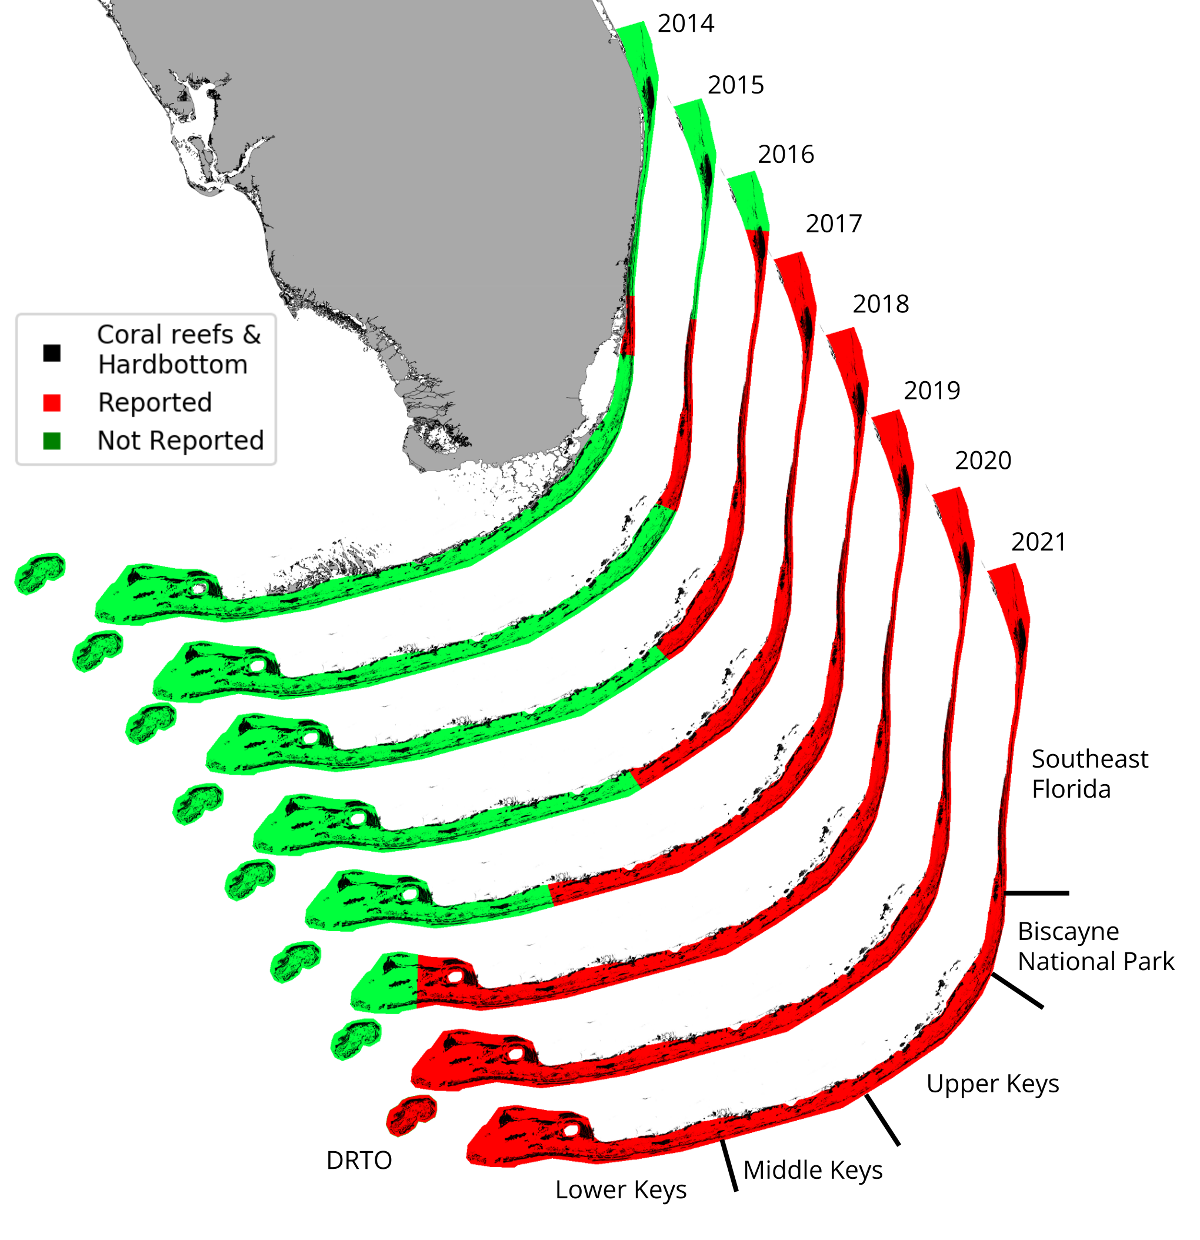
\includegraphics[width=\textwidth]{chapters/intro/figures/fig_sctld.png}
    \caption{Propagation of the SCTLD troughout the FRT between 2014 and 2021}
    \label{intro:propagation}
\end{figure}

\begin{figure}
    \centering
    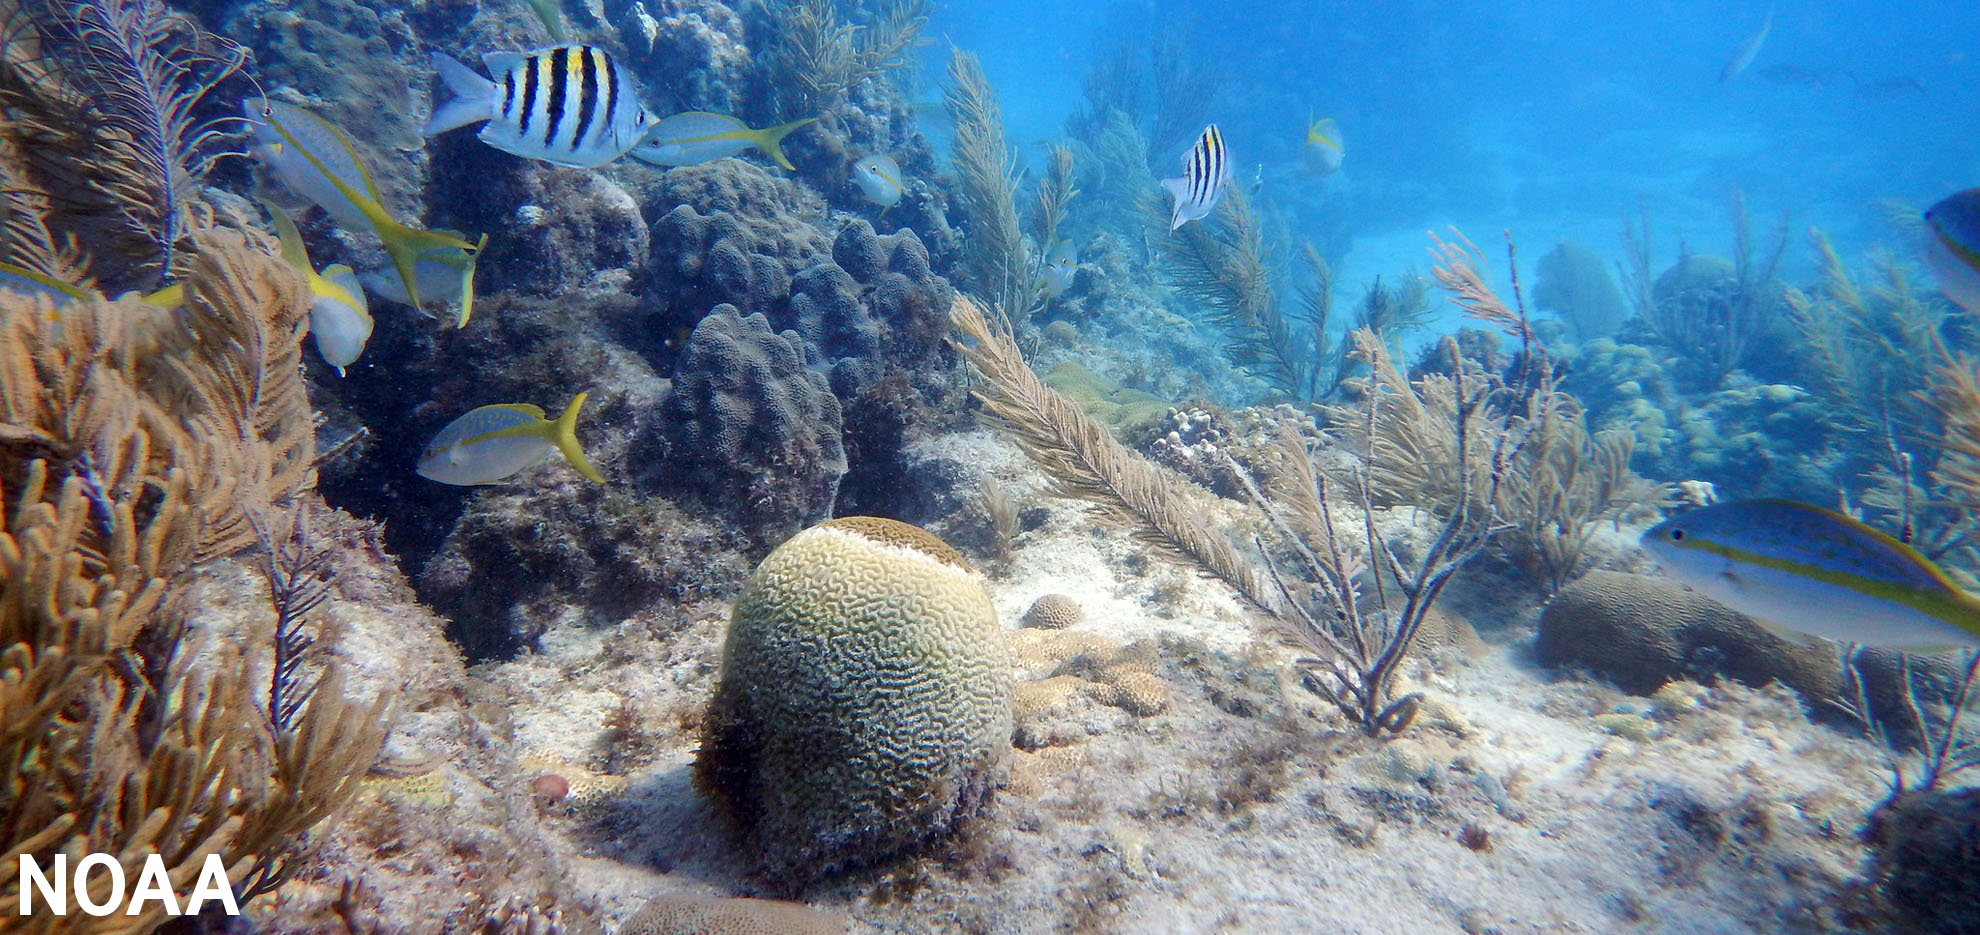
\includegraphics[width=\textwidth]{chapters/intro/figures/sctld.jpg}
    \caption{Brain coral affected by SCTLD in Looe Key, Florida. The disease is leaving a white band of recently dead skeleton in contrast to the healthy, yellow/brown tissue. Source: Florida Fish and Wildlife Research Institute}
    \label{intro:sctld}
\end{figure}

Additionally, Florida is a prime landfall target for tropical cyclones from June through November (Fig. \ref{inro:landfall}). Between 1899 and 1998, Southeastern Florida has been directly hit by 27 hurricanes, 5 of which were of category 4 or more (winds $>$ 209 km/h) \citep{neumann1999tropical}. Hurricanes that forms in June and July are usually weak while hurricanes occurring in August and September tend to become severe storms \citep{banks2008reef}. This is illustrated by Hurricane Irma, one of the strongest and costliest hurricanes on record in the Atlantic, that made landfall in Florida in September 2017 as a category 4 hurricane \citep{irmaNOAA, xian2018brief}. Hurricanes are a major agent of coral mortality in the Caribbean that contributed to the decline of acroporids \citep{gardner2003long,gardner2005hurricanes,aronson2001white}. They cause a wholesale destruction of the reef biota on their passage and can induce coral burial through sediment resuspension \citep{banks2008reef, miller2008effects, tweel2014contribution}. Furthermore, they significantly impact the content of surface waters through upwelling and mixing, which can disturb the benthic communities \citep{wachnicka2019hurricane,varlas2020investigating}. Moreover, heavy wind conditions generate important waves that interact with currents and significantly alter transport processes in nearshore waters \citep{niu2017role,mao2020particle}. This might impact the dispersion of coral larvae, that are released during the hurricane season \citep{hendee1998champ}. Hurricane might therefore interrupt larval exchanges between otherwise connected reefs but also create new connectivity pathways. As major hurricanes are intensifying under the effect global warming \citep{bhatia2019recent,knutson2020tropical}, better understanding the impact of hurricanes on wave-induced processes could inform the management of reefs under future climatic conditions. Furthermore, as incoming storm-generated waves dissipate over reefs, better understanding the protective role of coral reefs might promote their restoration as tool to reduce coastal flooding hazard \citep{roelvink2021coral}.

\begin{figure}
    \centering
    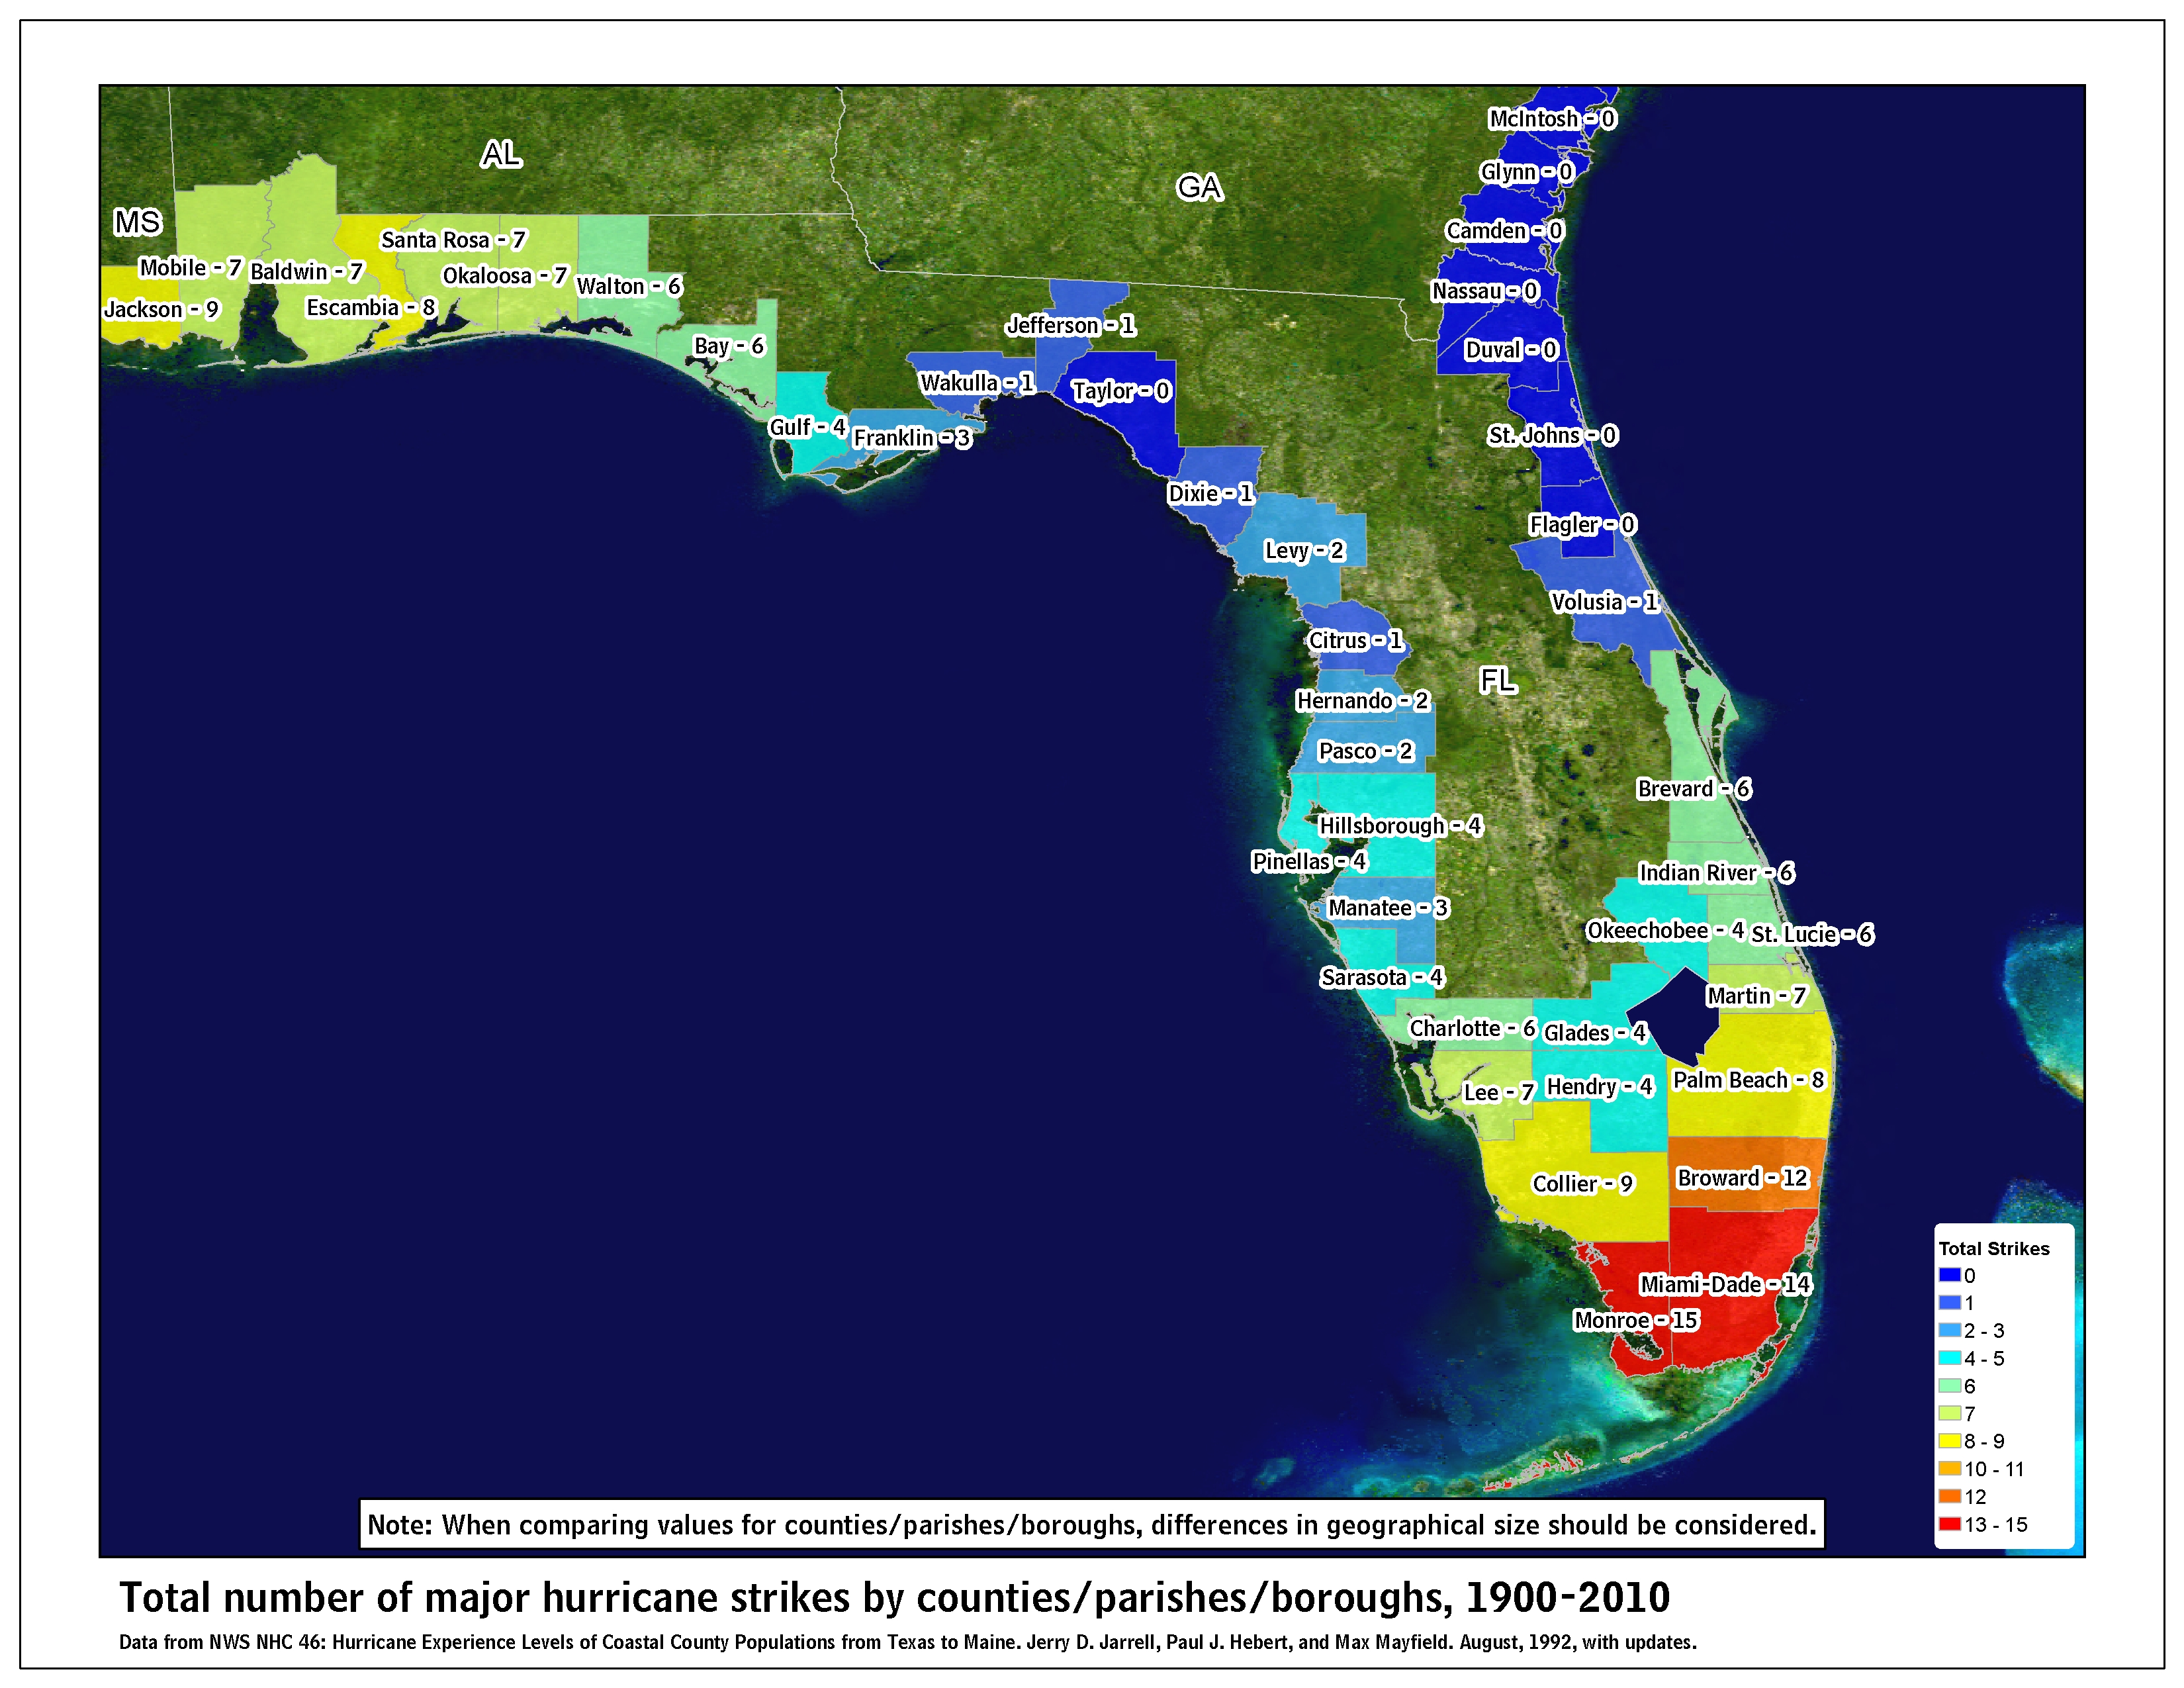
\includegraphics[width=\textwidth]{chapters/intro/figures/hurricane_strikes.jpg}
    \caption{Total number of major hurricanes strikes in Florida between 1900-2010. Source: National Oceanographic and Atmospheric Administration, National Hurricane Center \url{https://www.nhc.noaa.gov/climo/}}
    \label{inro:landfall}
\end{figure}

\section{Thesis objectives}

This thesis focuses on two main threats that could jeopardize the future and survival of FCR: the current outbreak of SCTLD and hurricanes. These threats were studied by fulfilling four main objectives. First, as SCTLD was expected to propagate through waterborne transmission, we developed a coupled epidemio-hydrodynamic model to reproduce the observed spread of the outbreak through the FRT. Such a model provides novel insight into the management of the epidemic, the identification of its causative agent, and its mode of transmission. Second, we used this model to explain the timing of the propagation of SCTLD within the FRT. More specifically, we investigated whether the modeled hydrodynamics were explanatory of the apparent stalling of the outbreak between the Marquesas and the DRTO in 2020. Third, as sediments can act as vector for the disease, we evaluated the impact of the PMDDP on the reported onset of SCTLD in 2014 using a sediment transport model. We assessed whether sediments produced or resuspended during dredging operations might have been transported to reefs where disease was reported and evaluated whether the timing of these sediment fluxes was consistent with the observed spread of the disease. Finally, we developed a coupled wave-current model to evaluate the impact of hurricanes on wave-induced transport processes. This model was applied to Irma, a major hurricane that made landfall in the Florida Keys in 2017, during the reproduction period of several coral species.

These objectives can be summarized into four main questions:
\begin{enumerate}
    \item How did the SCTLD spread through the FRT ?
    \item What caused the apparent stalling of the propagation of SCTLD ? 
    \item What was the impact of the PMDDP on the onset of the oubreak of SCTLD~?
    \item  What is the effect of hurricane-induced wave-current interactions on transport processes and should they be taken into account when modeling the dispersal of coral larvae ?
\end{enumerate}     
Answering these four questions required the use of an ocean model able to capture both the large-scale ocean features influencing circulation along the FRT as well as small-scale flow features down to the reef scale. A description of the main hydrodynamic features of the FRT as well as an overview of the modeling tools used in this thesis are given in the next section.

\section{Modeling hydrodynamics and transport processes in the FRT}
The FRT is located along the northern side of the Straits of Florida, that connects the Gulf of Mexico (GoM) and the North Atlantic Ocean. The large-scale circulation in this region is dominated by the interplay of the Florida Current (FC) and the Loop Current (LC). The LC is an area of warm waters from the Caribbean Sea that enters the GoM through the Yucatan Channel and then loops anti-cyclonically through the northeastern Gulf of Mexico and finally exits through the southern Straits of Florida, where it forms the Florida Current (FC). The FC then flows northward between Florida and the Great Bahama Bank to form the Gulf Stream (Fig. \ref{intro:gom}). The northward penetration of the LC through the GoM varies throughout the year, and sporadically an anticyclonic ring separates from the current \citep{leipper1970sequence, maul1977annual, vukovich1988loop}. The detachment of these anticyclonic eddies from the main LC affects in turn the position of the FC, causing its meandering along the FRT. These variations of the FC position have been shown to have no seasonal pattern with strong interannual variability. The generated meandering is associated with the presence of cyclonic eddies between the core of the current and the FRT \citep{kourafalou2012florida}. These eddies significantly impact the ecology of the southwest Florida Shelf by causing larval retention on the shelf and delivering larval pulses to the Upper Keys \citep{lee1994evolution, sponaugle2005florida, kourafalou2012florida}. Furthermore, when the LC meets the shallow waters of the southwest corner of the WFS near the DRTO, it causes the inflow of nutrients that modify water properties on the shelf \citep{weisberg2003local, liu2016offshore}. These contacts have been hypothesized to impact in turn the penetration of the LC in the GoM \citep{weisberg2017loop}. However, on the northernmost section of the FRT, eddies generated by the meandering of the FC cause cold-water upwelling limiting the northern range of tropical species \citep{walker2013determining}. The circulation on the upper part of the shelf along the FRT is largely influenced by winds, as well as diurnal and semi-diurnal tidal processes \citep{lee2001transport, lee2002volume,d2007patterns}

\begin{figure}
	\centering
	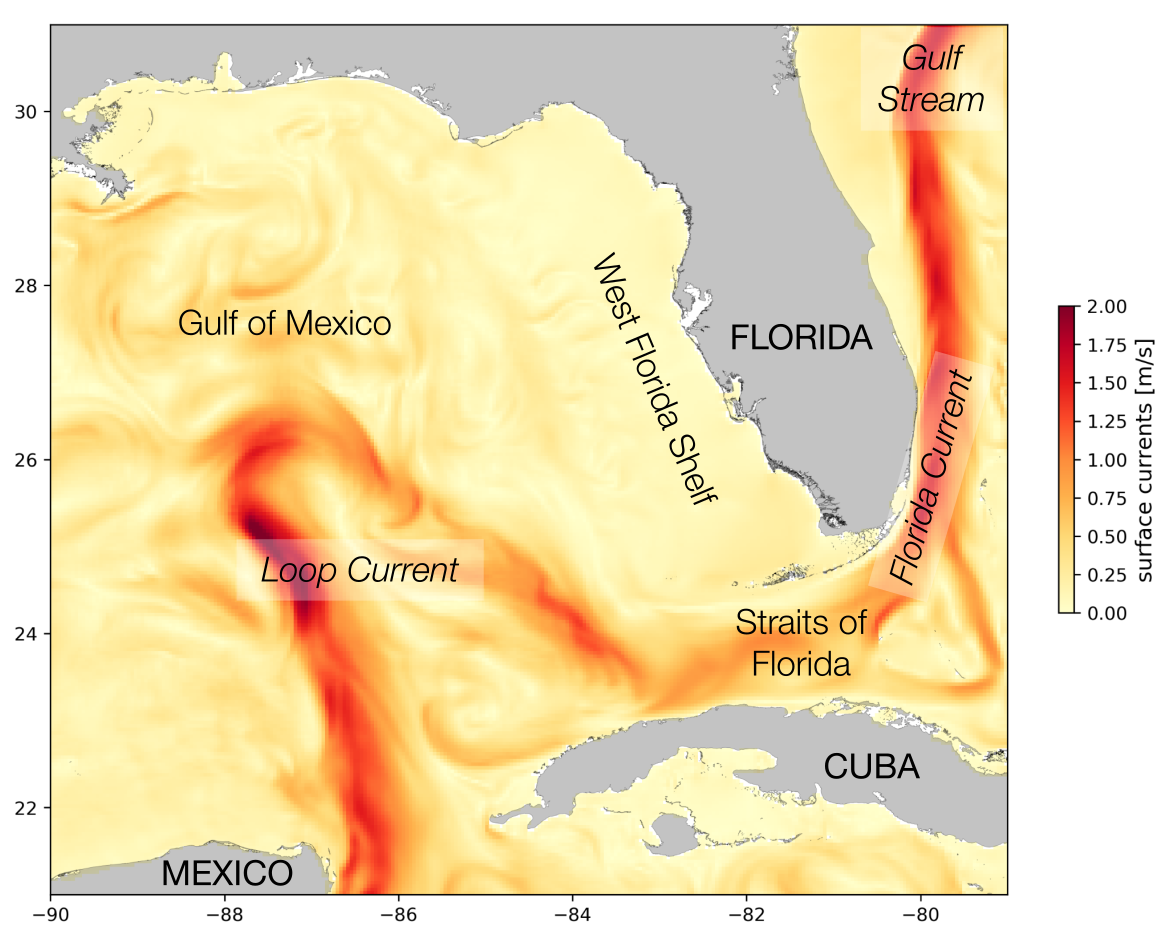
\includegraphics[width=.9\textwidth]{chapters/intro/figures/fig_gom.png}
	\caption{An example of the Loop Current and the Florida Current on January 12, 2019 as shown by HYCOM.}
	\label{intro:gom}
\end{figure}

The aforementioned large-scale ocean circulation significantly impact transport processes in the FRT. The modeling tools developed in this thesis should therefore be able to capture them accurately. Furthermore, as our objective is to model the dispersal of disease agents and sediments in a topologically complex coastal reef ecosystem, our modeling framework should also be able to capture small-scale ocean circulation features. For instance, small-scale flow features such as recirculation eddies around reefs and islands have been shown to strongly influence larval dispersal by increasing their local retention over the reefs \citep{figueiredo2013synthesizing}. Furthermore, accurately capturing the topography of coastal areas is critical when modeling storm conditions, as large wind waves generate strong currents, waves and storm surges in nearshore regions \citep{dietrich2010high, weisberg2006hurricane}. Unstructured-mesh models offer a well-suited solution to capture the multi-scale nature of flow features in the FRT in a computationally tractable way. They allow to locally increase the model resolution close to reefs and island while covering a domain large enough to capture the impact of the FC \citep{lambrechts2008multi,frys2020fine}. Nested grid models are another possible approach \citep{warner2010development} but they lack the flexibility required to adapt to the complex topology of coastal regions \citep{fringer2019future}. \todo{say something about HYCOM-GoM et HYCOM-FKeys...}

In this thesis, we used the 2D barotropic version of the unstructured-mesh Second-generation Louvain-la-Neuve Ice-ocean Model (\href{https://www.slim-ocean.be/}{SLIM}). This model relies on Discontinuous Galerkin finite element methods \citep{aizinger2002discontinuous} and has already been successfully used to model the hydrodynamics of the whole Great Barrier Reef \citep{lambrechts2008multi}. Moreover, by coupling SLIM with the HYbrid Coordinate Ocean Model (HYCOM-GOMl0.04, \citealp{chassignet2007hycom}), SLIM was able to indirectly represent the baroclinic dynamics of the FC. Using this coupling, \cite{frys2020fine} successfully modeled coral larval connectivity in the FRT, \ie~the exchanges of larvae between reefs. In this study, coral larvae were modeled using a Lagrangian particle tracking model forced by SLIM currents. To answer our different research questions, we adapted this larval transport model to evaluate the dispersal of the causative agent of the SCTLD and sediments particles.

At the beginning of this thesis, SLIM was not able to represent wave-current interactions under storm conditions. Heavy winds generate large wind-waves that disturb ocean conditions and interact non-linearly with the currents \citep{liu2020impacts,wu2011fvcom}. The wave-generated currents cause water level variations near shorelines and wave breaking points which, in turn, affect the motion and evolution of the waves \citep{longuet1970longshore, sikiric2013coupling}. Capturing wave-current interactions hence requires the calculation of the full directional wave spectrum in order to correctly reproduce the dynamics of wind-driven surface waves. This is usually achieved by spectral wave models, which describe the evolution of the wave energy spectrum. An objective of this thesis was therefore the coupling of SLIM with the spectral wave model Simulating WAve Nearshore (SWAN, \citealp{booij1999third}), specifically developed for coastal applications and relies on numerical schemes adapted to small-scale, shallow water regions. Further details on the models and their coupling is given in chapter \ref{chap:irma}.

\section*{Outline}
This thesis is mainly a collection of publications describing our answers to the four main research questions. Chapter \ref{chap:sctld} describes the development of a coupled epidemio-hydrodynamic model to reproduce the observed spread of SCTLD in the FRT. Chapter \ref{chap:drto} explains how this model was used to study the apparent stalling of the spread of the SCTLD between the Marquesas and the DRTO. Chapter \ref{chap:onset} investigates the impact of the PMDDP on the onset of the SCTLD oubreak in 2014. Chapter \ref{chap:irma} describes the development of a coupled wave-current model to study the impacts of Hurricane Irma (2017) on wave-induced transport processes in the Florida Keys. Finally, chapter \ref{chap:conclusion} presents the conclusions of this thesis and perspectives for further works. 

\newpage
\section*{Supporting publications}

\begin{list}{}{%
    \setlength{\topsep}{0pt}%
    \setlength{\leftmargin}{0.23in}%
    \setlength{\listparindent}{-0.23in}%
    \setlength{\itemindent}{-0.23in}%
    \setlength{\parsep}{\parskip}%
    }%
        
    \item \textbf{Dobbelaere, T.}, Muller, E. M., Gramer, L. J., Holstein, D. M., \& Hanert, E.
    (2020). Coupled epidemio-hydrodynamic modeling to understand the spread
    of a deadly coral disease in Florida. \textit{Frontiers in Marine Science}, 7, 1016. \href{https://www.frontiersin.org/articles/10.3389/fmars.2020.591881/full}{doi: 10.3389/fmars.2020.591881}
    
    \item \textbf{Dobbelaere, T.}, Curcic, M., Le Hénaff, M., \& Hanert, E. (2022). Impacts of Hurricane Irma (2017) on wave-induced ocean transport processes. \textit{Ocean Modelling}, 101947. \href{https://www.sciencedirect.com/science/article/pii/S1463500322000026}{doi: 10.1016/j.ocemod.2022.101947}
    
    \item \textbf{Dobbelaere, T.}, Holstein, D. M., Muller, E. M., Gramer, L. J., McEachron L., Williams, S. D., \& Hanert, E. (2022). Connecting the dots: Transmission of stony coral tissue loss disease from the Marquesas to the Dry Tortugas. \textit{Frontiers in Marine Science}, 9. \href{https://www.frontiersin.org/article/10.3389/fmars.2022.778938}{doi: 10.3389/fmars.2022.778938}.
    
    \item Purkis, S. J., Oehlert, A. M., \textbf{Dobbelaere, T.}, Hanert, E., \& Harris, P. (2020), Always a White Christmas in the Bahamas - Ocean Chemistry and Hydrodynamics Focus Winter Mud Production on Great Bahama Bank, \textit{Sedimentology}, in revision.
    
    \item Alaerts, L., \textbf{Dobbelaere, T.}, Gravinese, P. M., \& Hanert, E. (2022), Climate change will fragment Florida stone crab communities. \textit{Frontiers in Marine Science}, submitted.
    
    \item Hanert, E., Aboobacker, V.M., Veerasingam, S, \textbf{Dobbelaere, T.}, Vallaeys, V. \&
    Vethamony, P. (2021) A multiscale ocean modelling system for the central Arabian Gulf: From basin-scale circulation patterns to flow-structure interactions. \textit{Estuarine, Coastal and Shelf Science}, submitted.
    
    \item Lopez-Gamundi, C., \textbf{Dobbelaere, T.}, Hanert, E., Harris, P.,Eberli G., and Purkis, S. (2022) Simulating Sedimentation on the Great Bahama Bank – Sources, Sinks, and Storm. \textit{Sedimentology}. submitted.
    
    \item Anselain, T., \textbf{Dobbelaere, T.}, Heggy, E. \& Hanert, E. (2022) Qatar oil spill vulnerability threatens both its national water security and the global gas market. \textit{Nature Communications}, in preparation.
    
    \item Holstein, D. M., \textbf{Dobbelaere, T.}, Gramer, L. J., McEachron, L., Muller E. M., Williams, S. D. \& Hanert, E. (2022) Coral restoration in the age of emergent disease: Balancing the benefits and risks of population connectivity. \textit{Conservation Letters}. in preparation. 
    
\end{list}
\newpage 
\section{List of acronyms and abbreviations}

\begingroup
    \setlength{\tabcolsep}{20pt}
    \renewcommand{\arraystretch}{1.3}
    \begin{tabular}{ll}
        \textbf{DRTO}   & Dry Tortugas \\
        \textbf{ECMWF}  & European Centre for Medium-Range Weather Forecast \\
        \textbf{D55}    & Dredge 55 clamshell \\
        \textbf{FC}     & Florida Current \\
        \textbf{FCR}    & Florida's Coral Reef \\
        \textbf{FRT}    & Florida Reef Tract  \\
        \textbf{GoM}    & Gulf of Mexico \\
        \textbf{HURDAT} & HURricane DATabases \\
        \textbf{HYCOM}  & HYbrid Coordinate Ocean Model \\
        \textbf{LC}     & Loop Current \\
        \textbf{NOAA}   & National Oceanographic and Atmospheric Administration \\
        \textbf{ODMDS}	& Ocean Dredge Material Disposal Site \\
        \textbf{PoM}    & Port of Miami \\
        \textbf{PMDDP}  & PortMiami Deep Dredge Project \\
        \textbf{RS}     & Radiation stress \\
        \textbf{SB}     & Spider Barge \\
        \textbf{SCTLD}  & Stony coral tissue loss disease \\
        \textbf{SLIM}   & Second-generation Louvain-la-Neuve Ice-ocean Model\\
        \textbf{SWAN}   & Simulating WAves Nearshore \\
        \textbf{TI}     & Terrapin Island hopper \\
        \textbf{TX}     & Texas cutterhead \\
        \textbf{WWTP}	& Wastewater Treatment Plant \\
        \textbf{WFS}    & West Florida Shelf
    \end{tabular}
\endgroup    
%%
%%%%%% 
\mychapter{Modeling the spread of SCTLD in Florida} \label{chap:sctld}
\chaptermark{Modeling the spread of SCTLD in Florida}  

This chapter is based on the following article:
\begin{list}{}{%
\setlength{\topsep}{0pt}%
\setlength{\leftmargin}{0.23in}%
\setlength{\listparindent}{-0.23in}%
\setlength{\itemindent}{-0.23in}%
\setlength{\parsep}{\parskip}%
}%

\item \textbf{Dobbelaere, T.}, Muller, E. M., Gramer, L. J., Holstein, D. M., \& Hanert, E. (2020). Coupled epidemio-hydrodynamic modeling to understand the spread of a deadly coral disease in Florida. \textit{Frontiers in Marine Science}, 7, 1016. \href{https://www.sciencedirect.com/science/article/pii/S1463500322000026}{doi: 10.3389/fmars.2020.591881}.
\end{list}

\begin{abstract}
    For the last six years, the Florida Reef Tract (FRT) has been experiencing an outbreak of the Stony Coral Tissue Loss Disease (SCTLD). First reported off the coast of Miami-Dade County in 2014, the SCTLD has since spread throughout the entire FRT with the exception of the Dry Tortugas. However, the causative agent for this outbreak is currently unknown. Here we show how a high-resolution bio-physical model coupled with a modified patch Susceptible-Infectious-Removed epidemic model can characterize the potential causative agent(s) of the disease and its vector. In the present study, the agent is assumed to be transported within composite material (\textit{e.g.}~coral mucus, dying tissues, and/or resuspended sediments) driven by currents and potentially persisting in the water column for extended periods of time. In this framework, our simulations suggest that the SCTLD is likely to be propagated within neutrally buoyant material driven by mean barotropic currents. Calibration of our model parameters with field data shows that corals are diseased within a mean transmission time of 6.45 days, with a basic reproduction number slightly above 1. Furthermore, the propagation speed of the disease through the FRT is shown to occur for a well-defined range of values of a disease threshold, defined as the fraction of diseased corals that causes an exponential growth of the disease in the reef site. Our results present a new connectivity-based approach to understand the spread of the SCTLD through the FRT. Such a method can provide a valuable complement to field observations and lab experiments to support the management of the epidemic as well as the identification of its causative agent.
\end{abstract}

%\newpage



\section{Introduction}

Coral diseases are a major threat to coral reef ecosystems and have led to significant declines in coral cover especially within the Caribbean region  \citep{richardson1998florida, sutherland2004disease, aronson2001white, harvell2007coral, miller2009coral, brandt2009dynamics}. Indeed, the Florida Reef Tract (FRT), which was dominated by \textit{Acropora palmata} and \textit{Acropora cervicornis}, and often had ~30\% coral cover until the 1970s/80s \citep{dustan1987changes, porter1992quantification}, is now dominated by bare substrate, octocorals, and macroalgae with only approximately 5\% stony coral cover remaining \citep{ruzicka2013temporal}. The loss of the branching Acroporid species was attributed primarily to a disease outbreak, termed white band disease \citep{aronson2001white}, but several other threats such as habitat reduction, eutrophication, overfishing, hurricanes, and bleaching likely all contributed to these species decline \citep{acropora2005atlantic}. Subsequent losses of coral cover within the region were often linked to additional disease incidences and repeated regional coral bleaching events as a result of global climate change \citep{kuta1996abundance, richardson1998florida, sutherland2004disease, gardner2003long, aronson2006conservation, kuffner2015century, manzello2015rapid}. A novel coral disease outbreak, termed Stony Coral Tissue Loss Disease (SCTLD), is now threatening the last vestiges of coral throughout the Florida Reef Tract (FRT).

SCTLD was first documented off the coast of Miami-Dade County in the summer of 2014 by \cite{precht2016unprecedented} and has since spread throughout the entire FRT with the exception of the Dry Tortugas. To date, SCTLD has been observed affecting over 20 different stony corals species. A case definition of SCTLD has been compiled to describe the visual appearance and ecology of SCTLD \citep{noaa2018}. Briefly, the gross morphology of SCTLD is described as focal or multifocal, with locally extensive to diffuse areas of acute to subacute tissue loss distributed basally, peripherally, or both. In some cases, tissues bordering areas of chronic tissue loss show indistinct bands (1–5 cm) of pallor, progressing to normal pigmentation away from the denuded skeleton. There is also a range in coral susceptibility to SCTLD, with species categorized as highly susceptible (e.g., \textit{Dendrogyra cylindrus}, \textit{Dichocoenia stokesii}, \textit{Meandrina meandrites}), moderately susceptible (e.g., \textit{Orbicella} spp., \textit{Montastraea cavernosa}, \textit{Siderastrea siderea}, \textit{Stephanocoenia intersepta}), or tolerant (e.g., \textit{Porites} spp., \textit{Acropora} spp.). Unfortunately, SCTLD has not remained isolated in the FRT and has now been recorded in Mexico \citep{alvarez2019rapid}, the US Virgin Islands \citep{blondeau2020coral} and several other locations around the Caribbean \citep{kramer2019map}. The continued persistence of the outbreak, the high number of species affected, and the large geographical range of reports consistent with the case definition suggests that SCTLD is the largest coral disease outbreak on record 

Large-scale spatial epidemiologic analyses showed that the reefs in Florida with SCTLD are clustered, supporting a contagious mode of transmission \citep{muller2020spatial}. Similarly, aquaria-based experiments indicate SCTLD can be transmitted through direct contact or indirectly through the water column \citep{aeby2019pathogenesis} suggesting water can function as a SCTLD vector, at least within a controlled setting. The initial exponential increase in spread among reefs from the disease epicenter \citep{precht2016unprecedented} and the persistent subsequent linear rate of spread of SCTLD \citep{muller2020spatial}, north along South Florida reefs and south into the Florida Keys, indicates that water currents may play a role in disease transmission. Furthermore, the rate of spread, estimated at ~100 m per day, suggests surface currents are likely too fast to have spread SCTLD within the region. These results imply that either the middle layer or the bottom boundary layer, which are both significantly slower than surface currents, may be the vertical location in which transmission occurs \citep{muller2020spatial}. However, to date, there have been no attempt to link local hydrodynamic modeling efforts with the spatio-temporal dynamics of SCTLD in Florida.

Estimating the transport of the disease causative agent from reef to reef by currents cannot be performed empirically. However, experimentally-calibrated numerical models that simulate currents can provide a realistic picture of the dispersal of disease agents. Nonetheless, accurately modeling water circulation at the spatial scales that affect this dispersal remains a key challenge, as small-scale flow features such as recirculation eddies around reefs and islands strongly impact exchanges between reefs \citep{wolanski1994physical, burgess2007influence, figueiredo2013synthesizing}. In this context, models that can explicitly simulate flow features down to the reef scale are needed. This represents a spatial resolution of the order of 100-1,000 m in dense reef systems. As of today, most regional ocean models using traditional numerical methods cannot achieve such resolution because of the computational resources it requires. To our knowledge, the best resolution currently available among these models in the FRT is $\sim900$ m with the FKEYS-HYCOM model that has been developed for the Florida Keys region \citep{kourafalou2012florida, sponaugle2012observed, vaz2016perfect}. Unstructured-mesh ocean models offer a potential solution to this resolution issue by locally increasing the model resolution close to reefs and islands \citep{lambrechts2008multi, thomas2014numerical, thomas2015connectivity}, in order to focus the computational resources where they are most needed. High resolution bio-physical dispersal models can be used to build the potential connectivity between reefs and therefore approximate exchanges between colonies in the complex topography of the coral reef systems \citep{frys2020fine}.

Marine diseases differ significantly from better studied terrestrial diseases, namely due to the potential for long environmental residence times, during which pathogens may survive and disperse through the water \citep{harvell2007coral, sokolow2009editor}. Several recent studies have attempted to adapt traditional epidemic models (Susceptible-Infectious-Recovered, or SIR models) to coral reef systems \citep{sokolow2009editor, bidegain2016microparasitic, bidegain2016marine}. Novel approaches have included developing pathogen pools \citep{bidegain2016microparasitic, bidegain2016marine}, and to model at the metapopulation scale, rather than at the scale of coral holobionts \citep{sokolow2009editor}. Both of these approaches are attempting to address the same issue: disease occurs between patches of entirely sessile animals, through the dispersal of pathogen(s). Thus, there are internal within-patch disease dynamics and metapopulation-scale between-patch dynamics occurring simultaneously. The epidemic model developed in the present study utilizes the same basic architecture of previous coral reef SIR models, but rather than assume pathogen pools (e.g. \cite{bidegain2016microparasitic, bidegain2016marine}) or ignore internal patch dynamics (e.g. \cite{sokolow2009editor}), we have modeled both within-patch disease dynamics and the dispersal of pathogenic agents explicitly using potential connectivity networks.

The objective of the present study is to deduce the probable propagation mechanism of the SCTLD throughout the FRT by developing an experimentally-calibrated epidemio-hydrodynamic model. With a resolution of about 100 m, this model can capture potential exchanges of disease-carrying material, further denominated as "infectious" in our modeling framework, between reefs that would be ignored by coarser models. By reproducing the observed spread of disease between 1st May 2018 and 1st April 2019, we provide insight on the characteristics of the disease agent and its vector. Ultimately, our model, coupled with lab and field studies, provide novel insight into the management of the epidemic, the identification of its causative agent, and mode of transmission.

% === METHODS === %
\section{Methods}

% --> Subsection 1\dan{SIR modeling background:}
\subsection{Modeling reef connectivity}
In the present study, we focused on the exchanges of infectious material between coral reefs driven by ocean currents, which therefore have to be accurately simulated. An ocean model should provide a realistic large-scale circulation while also resolving small-scale flow features down to the scale of individual reefs. In this context, we used the unstructured-mesh depth-integrated coastal ocean model \slim\footnote{\url{https://www.slim-ocean.be}} to simulate ocean currents over an area that includes the FRT but also the Florida Strait and part of the Gulf of Mexico (Fig. \ref{fig:setup}). By using an unstructured mesh, we increased the model resolution only over the FRT and hence concentrate computational resources where they were most needed. \slim has already been successfully applied in complex coastal systems such as the Great Barrier Reef \citep{lambrechts2008multi, thomas2014numerical} and is well suited to shallow-water flows. Details of the model formulation and validation are provided in \cite{frys2020fine}. 

\begin{figure}
    \centering
    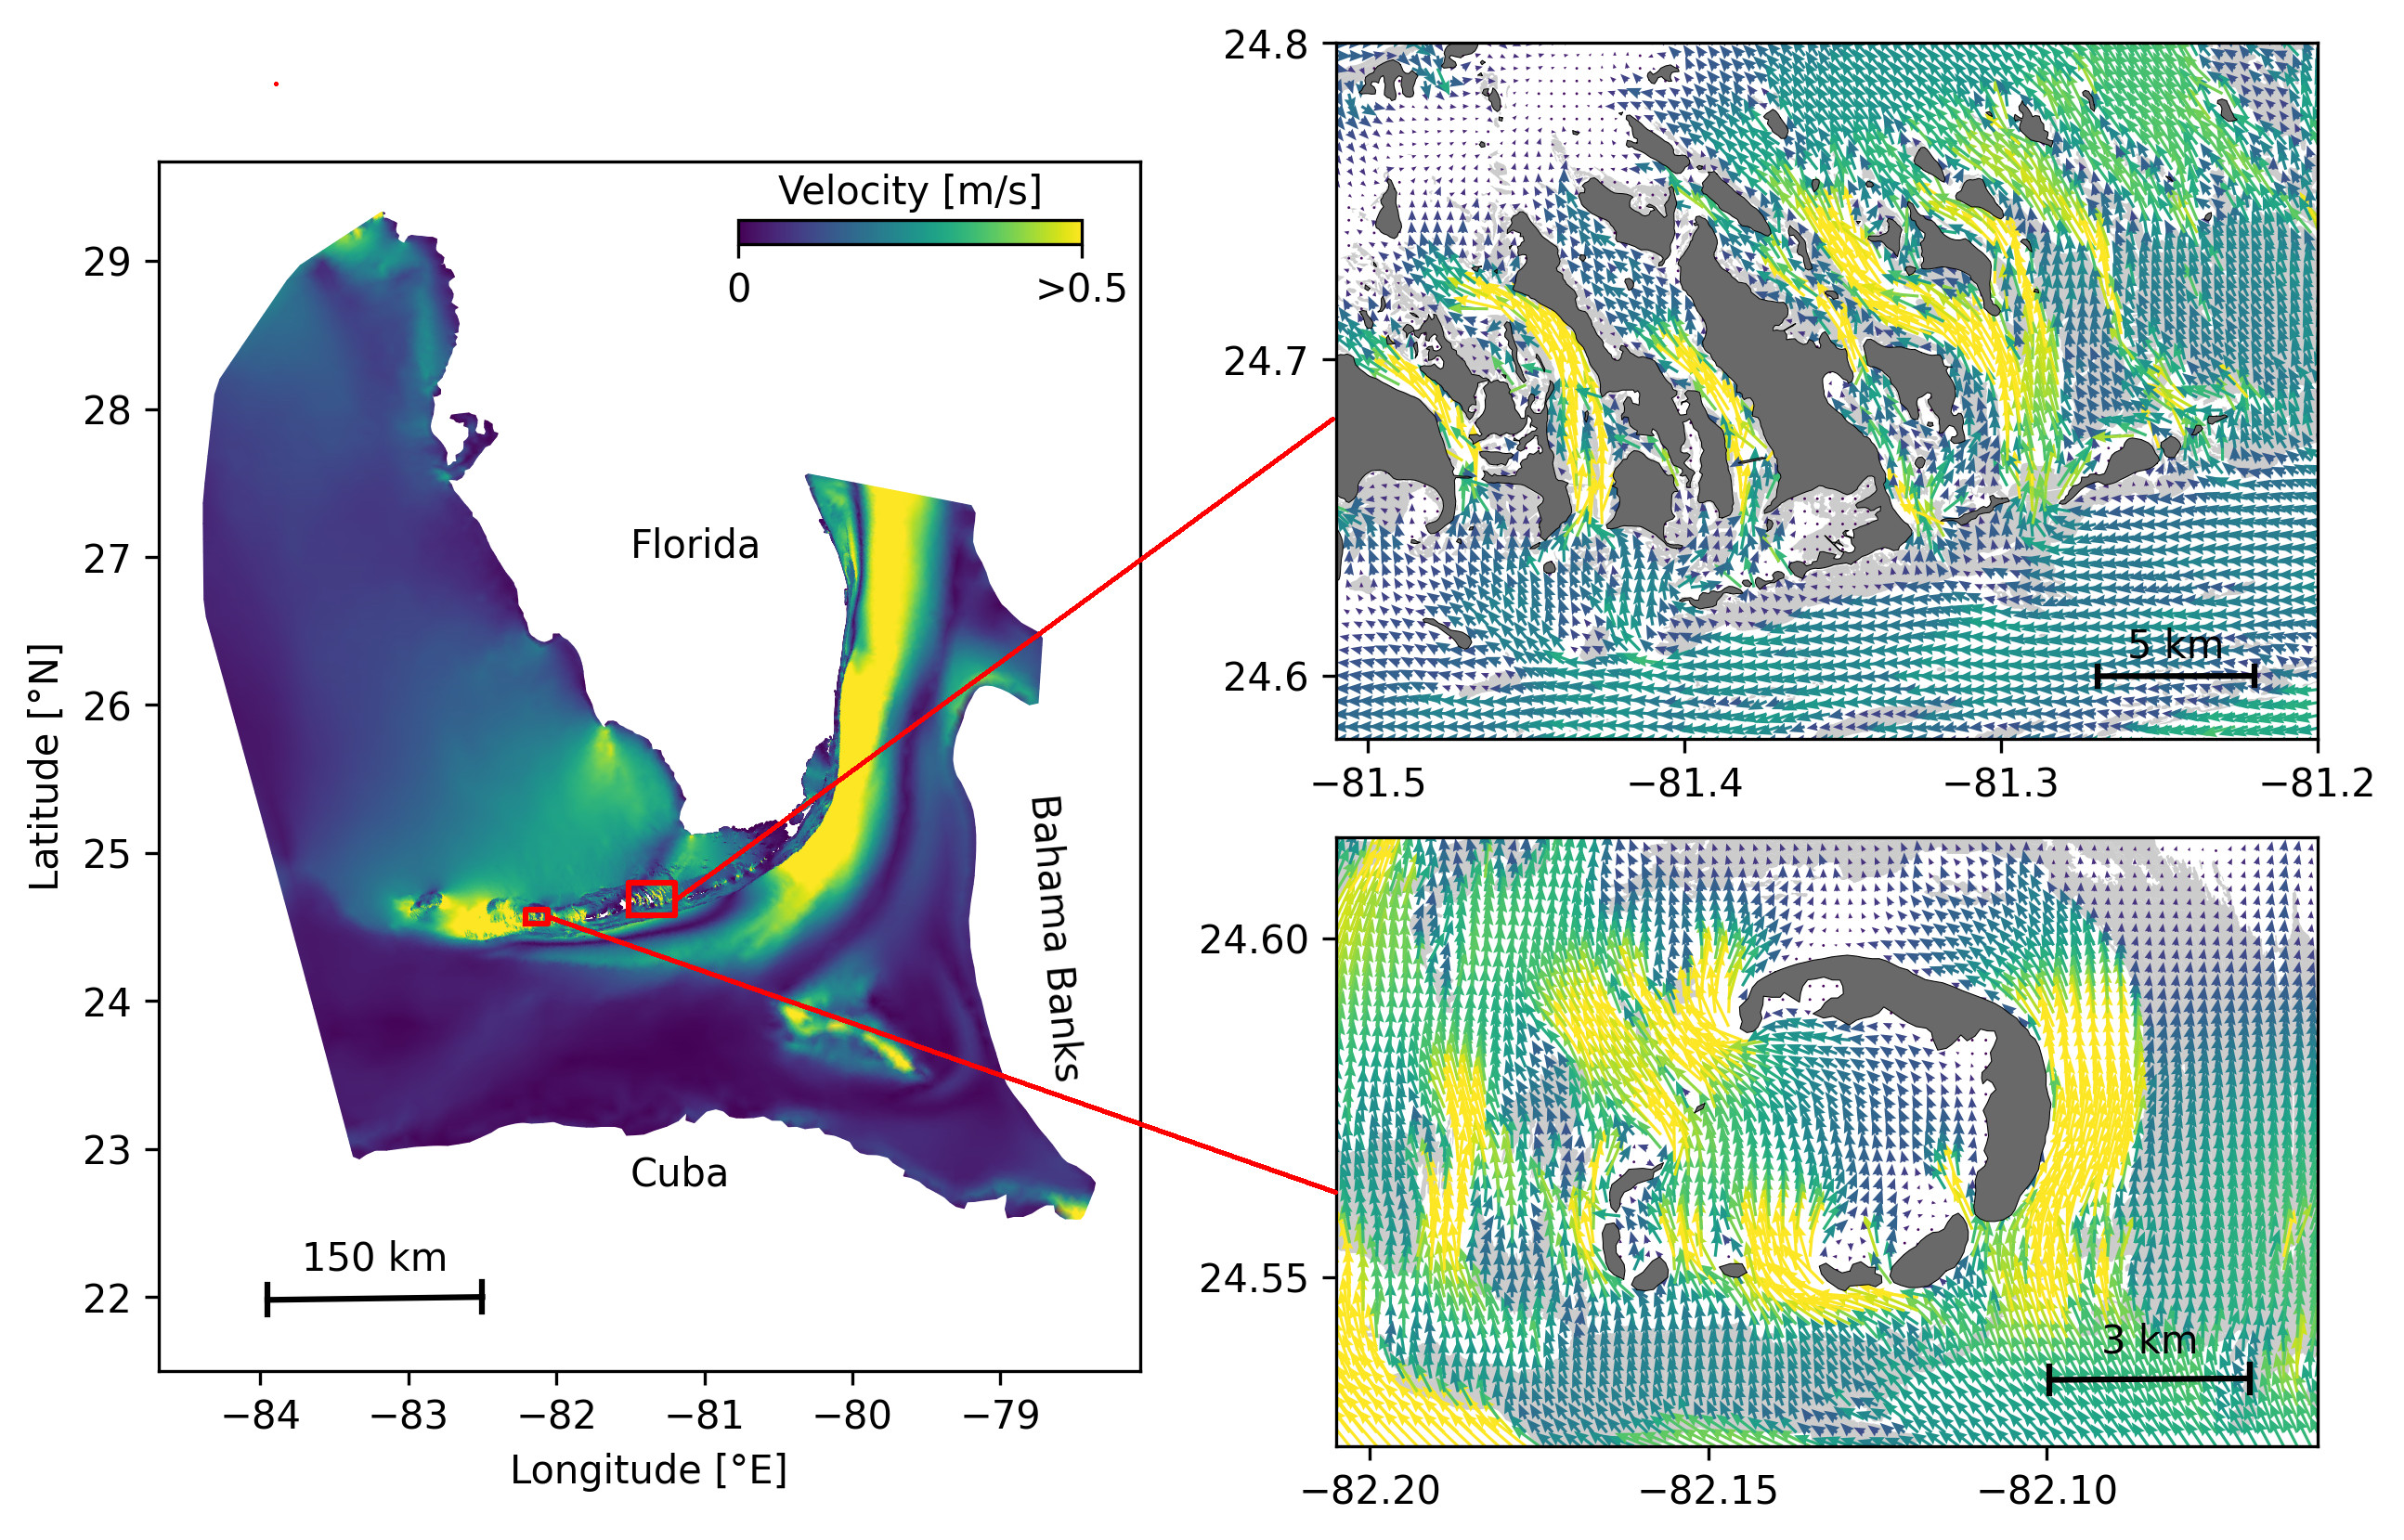
\includegraphics[width=.95\textwidth]{chapters/sctld/figures/vel.jpg}
    \caption{Model computational domain and close-up views of the mesh with snapshots of the currents on May, 25 2018 at 00:00, for the Marquesas Keys (bottom) and the Lower Keys (top). This illustrates the benefits of unstructured meshes to represent the fine-scale details of the topography and hence simulate currents down to the scale of individual reefs (shown in light grey) and islands (shown in darker grey).}
    \label{fig:setup}
\end{figure}

The mesh resolution depended only on the distance to the coast, but we distinguished between the coastlines along the FRT where we imposed a maximum resolution of 100 m and the other coastlines along which the finest resolution was 2500 m. The mesh was generated with the open-source mesh generator GMSH \citep{geuzaine2009gmsh} and is composed of approximately $7 \times 10^5$ elements. The coarsest elements, far away from the FRT, had a characteristic length size of about 10 km. Fig. \ref{fig:setup} depicts how a 100-m spatial resolution mesh simulated fine-scale details of the ocean currents, such as recirculation eddies and currents within the dense reef system in the Lower Keys that consist of many individual reefs with narrow passages in between. 

The simulated currents were then used to model dispersal of disease agents throughout the FRT. In this study, 3 types of potential vectors carrying the disease causative agent were considered: positively buoyant (e.g. mucus and surfactant), neutrally buoyant (e.g. fines, pelagic organisms) and negatively buoyant (e.g. sediments, composites, demersal organisms). As SLIM is a depth-averaged model, the mean currents it generates are well suited to model the dispersal of neutrally buoyant material remaining within the water column. However, these currents must be modified to correctly represent the dynamics of material evolving in the surface and bottom boundary layers. Therefore, surface current response to winds was estimated by adding 1.5\% of the wind speed to SLIM currents with a stress-layer veering angle of 45$^\circ$ to the right for positively buoyant particles. Such parameterization is shown to be an accurate approximation of wave-induced Stokes drift and quasi-Eulerian surface currents by \cite{ardhuin2009observation}. For negatively buoyant material, bottom currents were obtained by taking 60\% of SLIM currents velocity with a veering angle of 15$^\circ$ to the left. This is an approximation based on observations of bottom currents and whole water column current profiles in the shallow waters ($<$15 m) of Hawk Channel in the middle Florida Keys by \cite{smith2009influence}, as well as observations obtained during the Atlantic Ocean Acidification Testbed project (Gramer, pers. comm.). This application is also consistent with the theory of current veering in the bottom Ekman layer, albeit that was previously observed in deeper (30-90 m) coastal waters, e.g., by \cite{perlin2007organization} and \cite{kundu1976ekman}.

Using these three velocity fields, virtual particles were then released on all the reefs composing the FRT to model the dispersal of material carrying the disease causative agent. The locations of the reefs of Florida were extracted from the "coral reefs and hardbottom" layer of the Unified Florida Reef Tract Map \citep{fwc2017unified}. The polygons of this reef map were then further divided into 500 m $\times$ 500 m squares in order to track the propagation of the disease with a finer geographical resolution, generating a total of 16,823 polygons. At the beginning of each simulated month and for each type of current, a total of about $1.5 \times 10^6$ particles were released over all the reef polygons. These particles had a state composed of their polygon of origin as well as their mass, that they lose at a constant rate $\gamma$ as they were moved by surface, mean or bottom currents. The value of $\gamma$ was chosen so that particles had a half-life of 30 days. When the particles were brought over a reef polygon by currents, the amount of disease mass that landed on the polygon was recorded in monthly potential connectivity matrices, whose entries are denoted $C_{ij}$. The matrix rows correspond to the source reefs and the columns correspond to the destination reefs. Hence $C_{ij}$ represents the mass of diseased material originating from sub-reef $i$ that had settled on sub-reef $j$. This matrix was then normalized by dividing each of its rows $i$ by the total mass of particles released on polygon $i$ in order to obtain the normalized potential connectivity matrix $\tilde{C}$, whose entry $\tilde{C}_{ij}$ gives the probability that disease agents produced on sub-reef $i$ settle on sub-reef $j$. Connectivity matrices were computed for each type of current and for each month of the simulated period.

These connectivity matrices are more easily handled by interpreting them as large graphs whose vertices are sub-reefs and whose edges represent connectivity pathways. They were analyzed using graph theory tools. In the present study, four potential connectivity measures were used to interpret the monthly computed graphs. These indicators are described in Table \ref{tab:indicator}. The first indicator is the weighted connectivity length (WCL), which gave the average dispersal distance from origin to destination for material produced on a given reef. The weighted connectivity of reef polygon $i$ is expressed as:
\begin{equation}
    \textrm{WCL}_i = \dfrac{\sum_j \tilde{C}_{ij} L_{ij}}{\sum_j \tilde{C}_{ij}}
\end{equation}
where $L_{ij}$ is the distance between origin reef $i$ and destination reef $j$. Another measure of the spreading potential of reef $j$ is its out-degree, \ie the product of the number of connections originating from reef $j$ by the quantity of disease agents it sent to the network. This indicator was obtained by computing the number of non-zero entries of row $i$ in the potential connectivity matrix $C$ and multiplying it with $\sum_j C_{ij}$. The information given by the out-degree was complemented by the fraction of disease agents produced on reef $i$ that successfully settled on a reef, called the fraction exchanged of reef $i$. This indicator is given by $\sum_{j} \tilde{C}_{ij}$. Finally, the isolation of reef $i$ in the network was given by its self-recruitment, \ie the fraction of disease agents settling on reef $i$ that originated from reef $i$, computed by $C_{ii}/\sum_jC_{ji}$. A large self-recruitment value indicates that little infectious material produced elsewhere settled on the reef and thus that it was isolated from the rest of the network. However, due to its relative nature, high self-recruitment could still be coupled with a large amount of exogenous diseased agents reaching the reef, although this quantity would be considered proportionally small in regard to the total mass of diseased material settling on the reef.

\begin{table}
    \centering
    \begin{tabular}{|p{3cm}|p{4cm}|p{3.5cm}|}
        \hline
        \textbf{Indicators} & \textbf{Description} & \textbf{What it shows} \\
        \hline
            Weighted connectivity length (WCL) & 
            Average dispersal distance from origin to destination reef for all disease agents released over a reef & 
            Average distance that disease agents from a reef travels successfully to another reef \\
        \hline
            Out-degree &
            Number of out-going connections originating from a given reef multiplied by the total mass exchanged  &
            Overall potential for a reef to spread the disease \\
        \hline
            Fraction exchanged &
            Fraction of disease agents produced on a given reef that settles on other reefs &
            Relative likelihood of successful spread of the disease to other reefs  \\
        \hline
            Self-recruitment &
            Fraction of disease agents settling on a given reef that has been released on the same reef &
            Relative likelihood of unsuccessful spread of the disease from other reefs \\
        \hline            
    \end{tabular}
    \caption{Indicators used to analyze the modeled exchanges of infected material for each considered type of currents and for each simulated month.}
    \label{tab:indicator}
\end{table}

% --> Subsection 2
\subsection{Epidemiological modeling}

\subsubsection{Model equations}

The spread of the SCTLD throughout the FRT was simulated using a connectivity-based \cite{kermack1927contribution} SIR model. SIR models are among the most standard epidemiological models. They divide individuals into three compartments: susceptible ($S$), infectious ($I$) and removed ($R$). When affected by the disease, susceptible individuals become infectious and infect other susceptible individuals until they are removed from the system, either through recovery or death. Such models usually rely on the hypothesis of an homogeneous, well-mixed population. To account for the spatial heterogeneity of the FRT, the basic SIR formulation was modified by considering the fractions of susceptible ($S_j$), infectious ($I_j$) and removed ($R_j$) corals of each sub-reef $j$. Although the pathogen of SCTLD has not been identified, studies suggest a contagious mode of transmission \citep{aeby2019pathogenesis,muller2020spatial}. Here, we use 'infectious' to denote disease agents that could be passed from individual to individual, which are responsible for causing disease signs. We note that the disease agents could be biological or non-biological in nature. In the present study's epidemiological model, individual reefs interact through the exchange of disease agents as represented by the different connectivity matrices. For each sub-reef $j$ and at any time, the following relations hold: $0\leq S_j,I_j,R_j\leq 1$ and $S_j+I_j+R_j=1$. The evolution of these fractions through time is governed by the following equations:
\begin{equation}
    \begin{aligned}
        \dfrac{dS_j}{dt} &= -\beta\sum_i\dfrac{A_i}{A_j}I_i\tilde{C}_{ij}S_j - \beta'(I_j)S_jI_j \\
        \dfrac{dI_j}{dt} &= \beta\sum_i\dfrac{A_i}{A_j}I_i\tilde{C}_{ij}S_j + \beta'(I_j)S_jI_j - \sigma I_j \\
        \dfrac{dR_j}{dt} &= \sigma I_j
    \end{aligned}\label{eq:epidemio}
\end{equation}
where $\tilde{C}_{ij}$ is the entry corresponding to reef pair $(i,j)$ of the normalized potential connectivity matrix [-], $A_i$ is the area of reef polygon $i$ [km$^2$], $\sigma$ is the mortality rate [day$^{-1}$], and $\beta$ and $\beta'(I_j)$ are the inter- and intra-reef disease transmission rates [day$^{-1}$], respectively. In this model, diseased corals of sub-reef $i$ can 'infect' corals of sub-reef $j$ if there is non-zero probability of disease agents exchange from sub-reef $i$ to sub-reef $j$, given by $\tilde{C}_{ij}$. Moreover, to account for coral resistance to the disease, the intra-reef transmission function $\beta'(I_j)$ has the shape of a smooth step function of the fraction of infectious corals $I_j$ and is expressed as follows:
\begin{equation}
    \beta'(I_j) = \dfrac{\beta_0'}{2}(1+\tanh[(I_j-I_0)/\tau]),\label{eq:beta}
\end{equation}
where $I_0$ is a threshold on the infection population above which intra-reef transmission becomes significant, and $\tau$ is a measure of the interval over which the transition from low to high transmission occurs. As long as the fraction of infectious corals on sub-reef $j$ is below $I_0$, the only infection mechanism taking place is connectivity-driven transmission at rate $\beta$. Once the threshold is approached, intra-reef transmission with rate $\beta'_0$ is activated. A larger value of threshold $I_0$ corresponds to a greater resistance of corals to the disease, and therefore a slower spread of the disease within reef $j$. Coral reproduction and natural (\ie non SCTLD-related) death rates are not taken into account in this model, which amounts to assume that they balance each other. For this study the same values were used for $\beta$ and $\beta'_0$.
%This assumption seems reasonable since coral populations of the FRT were declining prior to the emergence of the SCTLD outbreak. 

\subsubsection{Calibration}

Transmission and removal parameters $\beta_0'$ and $\sigma$ were fitted to disease prevalence observations averaged over all colonies from 6 permanent monitoring sites in the Lower Keys to accurately simulate the temporal evolution of $S_j,I_j,R_j$ on each diseased reef polygon. Three focal reef sites were established in the lower Florida Keys, one offshore (Acer 17/18), one mid-channel (Wonderland), and one nearshore reef (N. Birthday). Sites were established in May 2018, when all colonies appeared healthy. Within each site, two 10 m $\times$ 10 m quadrats were established. Quadrats were generally set up from east to west although N. Birthday was established with one quadrat further north of the other two to better capture coral cover in the site. All coral colonies $>$ 10 cm in size were mapped using self-contained underwater breathing apparatus (SCUBA). Each coral was given an $(x,y)$ coordinate, identified to species, and maximum diameter was noted. After the initial data collection surveys, each site was visited every two to three weeks for rapid assessments to determine whether SCTLD was present. During these site visits, two divers conducted a visual assessment at each of the 6 quadrats. Disease was first observed in early October 2018. Detailed surveys were conducted every two to four weeks until December 2019. During the surveys, each individual coral was visually assessed for signs of SCTLD, including discoloration and tissue loss. Prevalence of diseased, apparently healthy, and dead were assessed for each time period. To relate our model framework to the compiled data, Eqs. $\ref{eq:epidemio}$ were simplified to a single-reef SIR model:
\begin{equation}
    \begin{aligned}
        \dfrac{dS}{dt} &= -\beta'_0SI \\
        \dfrac{dI}{dt} &= \beta'_0SI - \sigma I \\
        \dfrac{dR}{dt} &= \sigma I
    \end{aligned}\label{eq:simplified}
\end{equation}
Due to the low values of the entries in the normalized connectivity matrix $\tilde{C}_{ij}$, intra-reef transmission, when activated, is the dominant infection mechanism of Eqs. \ref{eq:epidemio}. Consequently, Eqs. \ref{eq:simplified} gave a reasonable approximation of the evolution of the disease on sub-reefs for which $I_j \geq I_0$. Using this approximation, the ratio $\beta_0'/\sigma$ was estimated by matching the modeled fraction of susceptible corals remaining after the disease activity had stopped ($S_\infty$) with observations. A standard property of a SIR model solution is such that
\begin{equation}
    S_\infty - \frac{\sigma}{\beta_0'}\log(S_{\infty}/S(t=0)) = 1\label{eq:ratio}
\end{equation}
where the initial fraction of susceptible corals ($S(t=0)$) was taken equal to $1-I_0$ (see for instance \cite{Murray07}). In the framework of Eqs. \ref{eq:simplified}, the ratio $\beta_0'/\sigma$ gave the value of the basic reproduction number $R_0$, defined as the average number of secondary cases produced by one infected individual introduced into a population of susceptible individuals \citep{keeling2007stochastic}. This number is used in epidemiological models to determine whether an emerging infectious disease can spread in a population ($R_0 > 1$) or not ($R_0 < 1$). The basic reproduction number that was obtained was then used to express $\sigma$ in terms of $\beta_0'$ and calibrate its value to reproduce, as well as possible, the temporal evolution of the colonies-averaged susceptible population shown in Fig. \ref{fig:calibration}.

\subsubsection{Initialization} \label{sec:init}

In order to solve Eqs. \ref{eq:epidemio}, initial conditions were needed, \ie fractions of susceptible, infectious and recovered corals at the beginning of the simulated period. This information was constructed from 9 different field-collected datasets: (i) Coral Reef Evaluation and Monitoring Project (CREMP; 2014–2017), (ii) CREMP Presence/Absence Data (CREMP P\_A; 2016–2017), (iii) Southeast Florida Coral Reef Evaluation and Monitoring Project (SECREMP; 2014–2017), (iv) Florida Reef Resilience Program Disturbance Response Monitoring (FRRP; 2014–2017), (v) Hurricane Irma Rapid Reef Assessment (IRMA; 2017, \cite{viehman2018}), (vi) the Southeast Florida Action Network citizen science program (SEAFAN; 2014–2017), and (vii) the Southefrn Coral Disease Margin field effort (2017 and 2018; \cite{neely2018surveying}), (viii) Mote Marine Laboratory’s Field operations data (2018-2019) and (ix) data compiled through the citizen science BleachWatch program (2018). Every dataset provided data on the presence or absence of the SCTLD (or tissue loss consistent with the SCTLD case definition) within each survey. Some also provided detailed disease metrics such as the species affected and the disease prevalence, which was subsequently compiled into presence/absence of SCTLD data by surveyed site. The locations of these observations are shown in Fig. \ref{fig:stns}. Using this information, we first delineated the diseased zone by constructing the concave hull of the points where the disease was observed before May 2018. The reefs diseased prior to the beginning of our simulated period were then defined as the reefs located inside the constructed zone. The time of disease observation was then spatially interpolated on each reef of the diseased zone by kriging with a Gaussian semivariogram using Python \texttt{pyKrige} module \citep{murphy2014pykrige}. Assuming an initial state $(S,I,R)=(1-I_0, I_0, 0)$ when the disease was observed, the fractions of susceptible, infectious and removed corals on each reef of the diseased zone on the 1st May 2018 was finally approximated using Eqs. \ref{eq:simplified}. Reefs outside of the diseased zone were initialized with an entirely susceptible population.  

\begin{figure}
    \center
    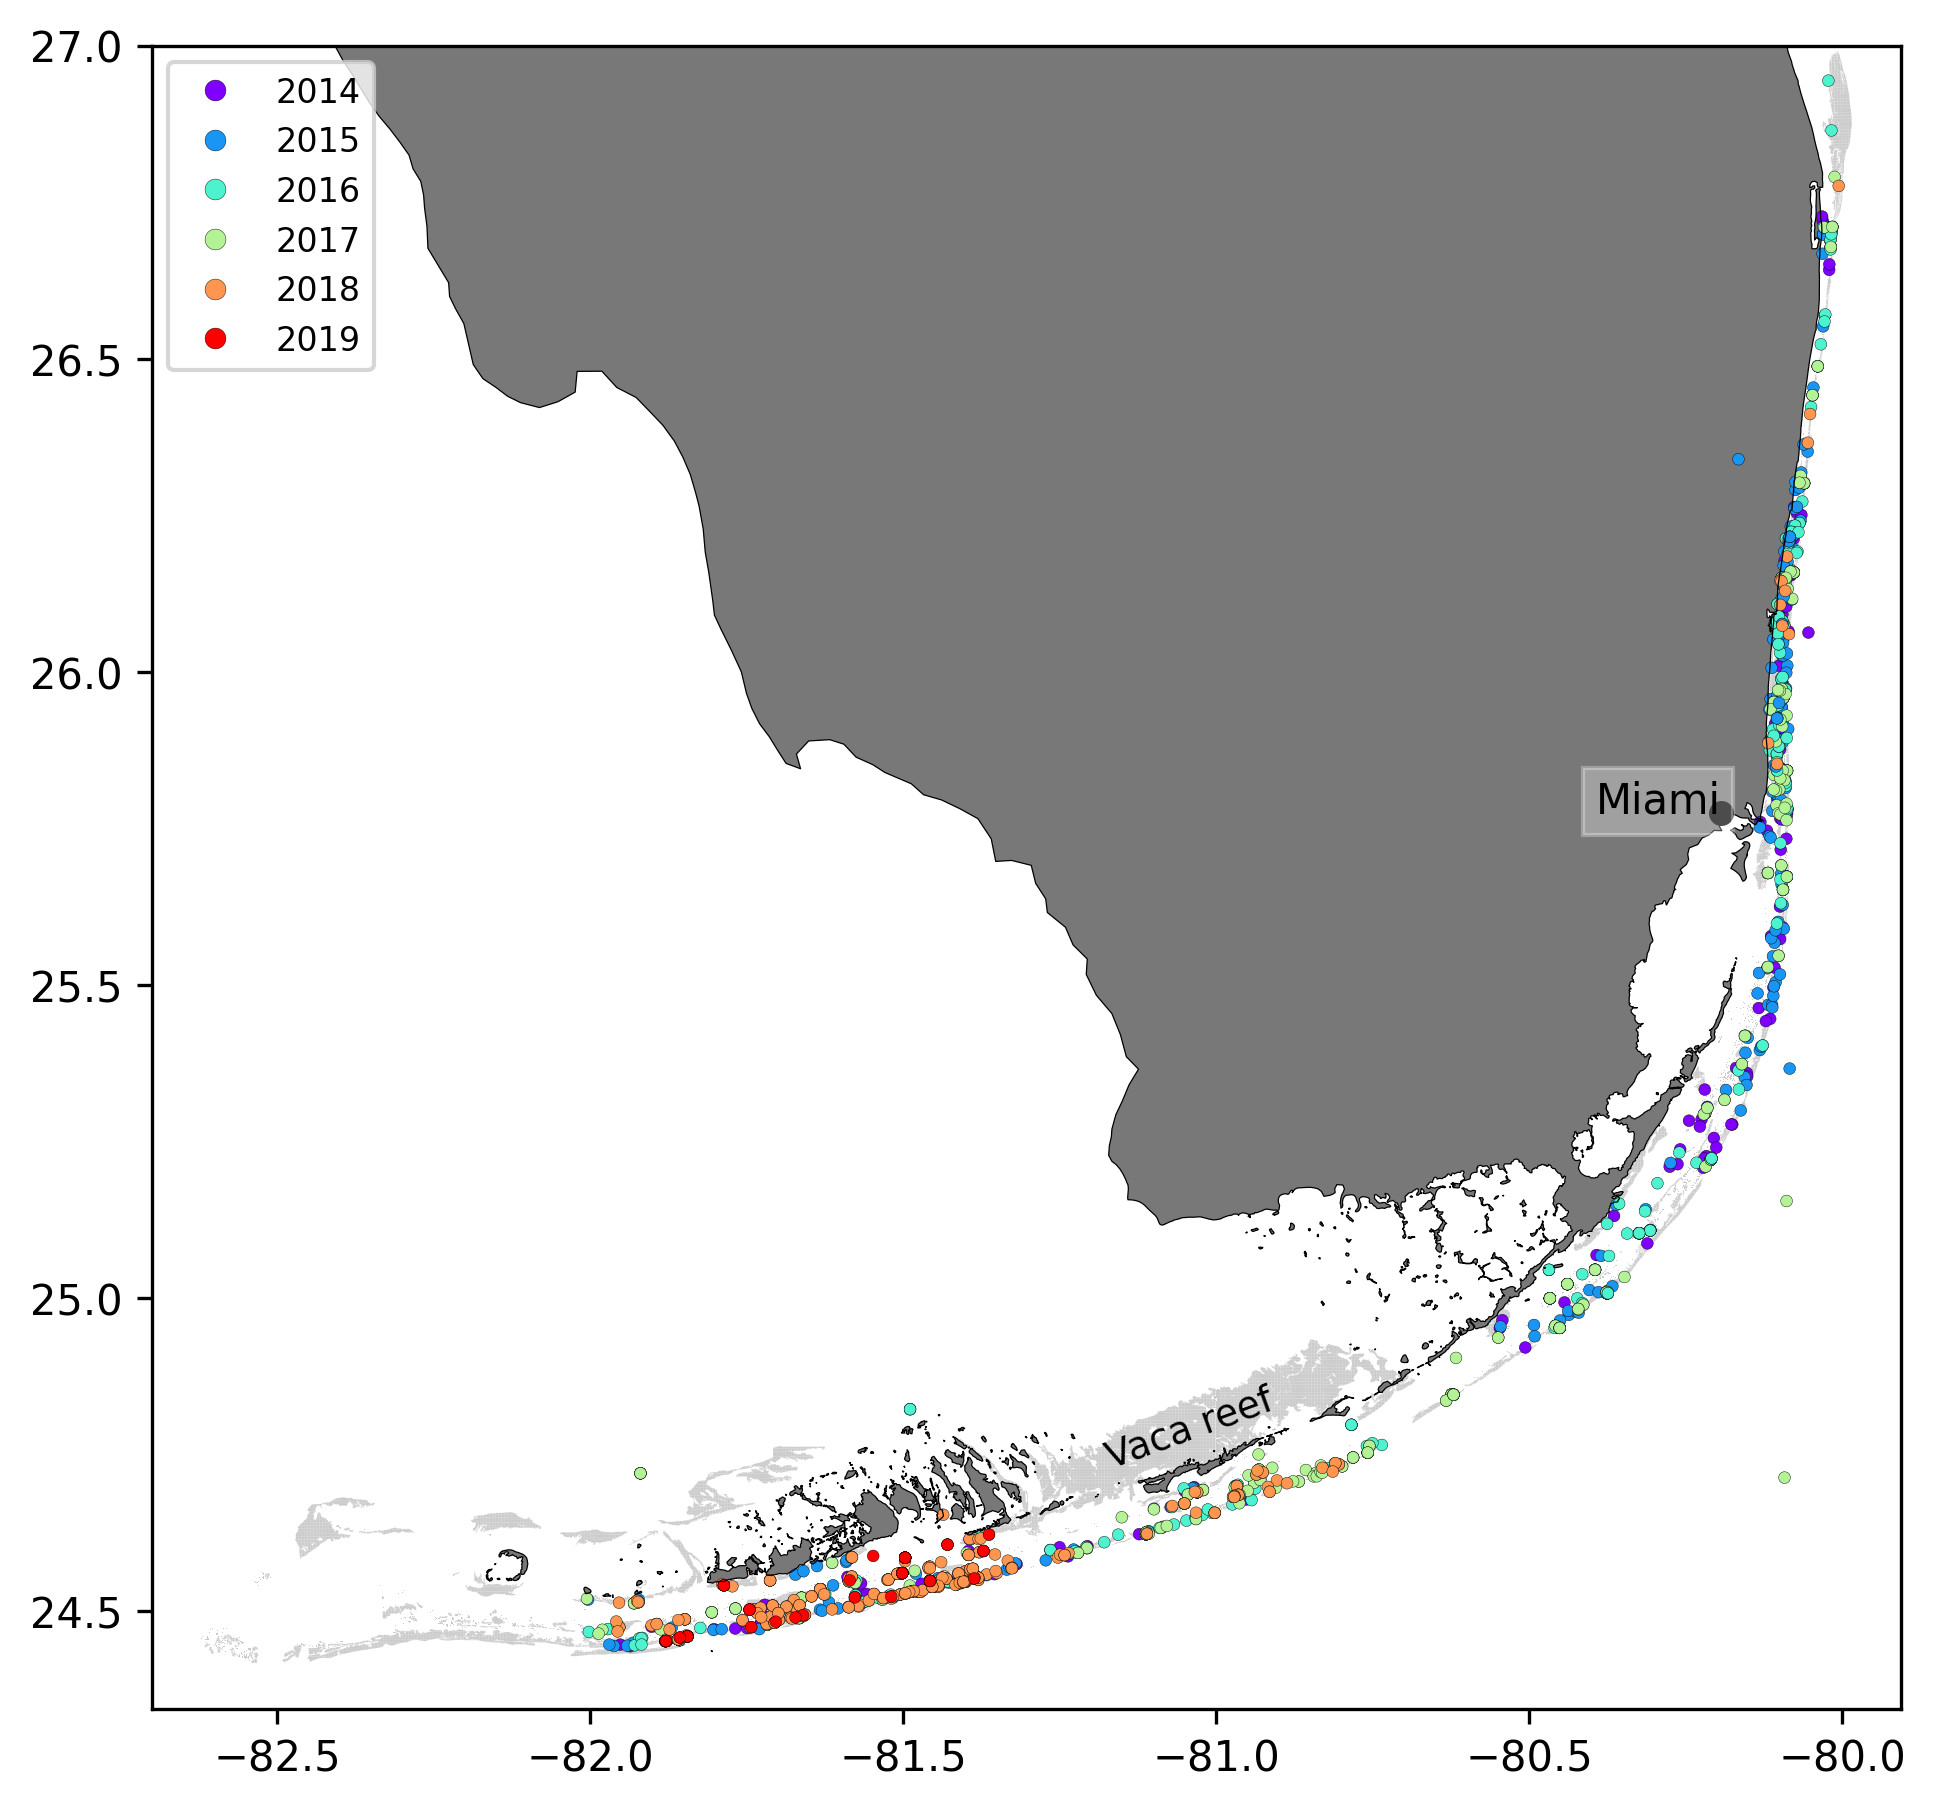
\includegraphics[width=.8\textwidth]{chapters/sctld/figures/monitoring.jpg}
    \caption{Locations of the disease observations between 2014 and 2019 recorded in the data sets used in this study.}
    \label{fig:stns}
\end{figure}

\subsubsection{Computation of front speed}

\begin{figure}
    \centering
    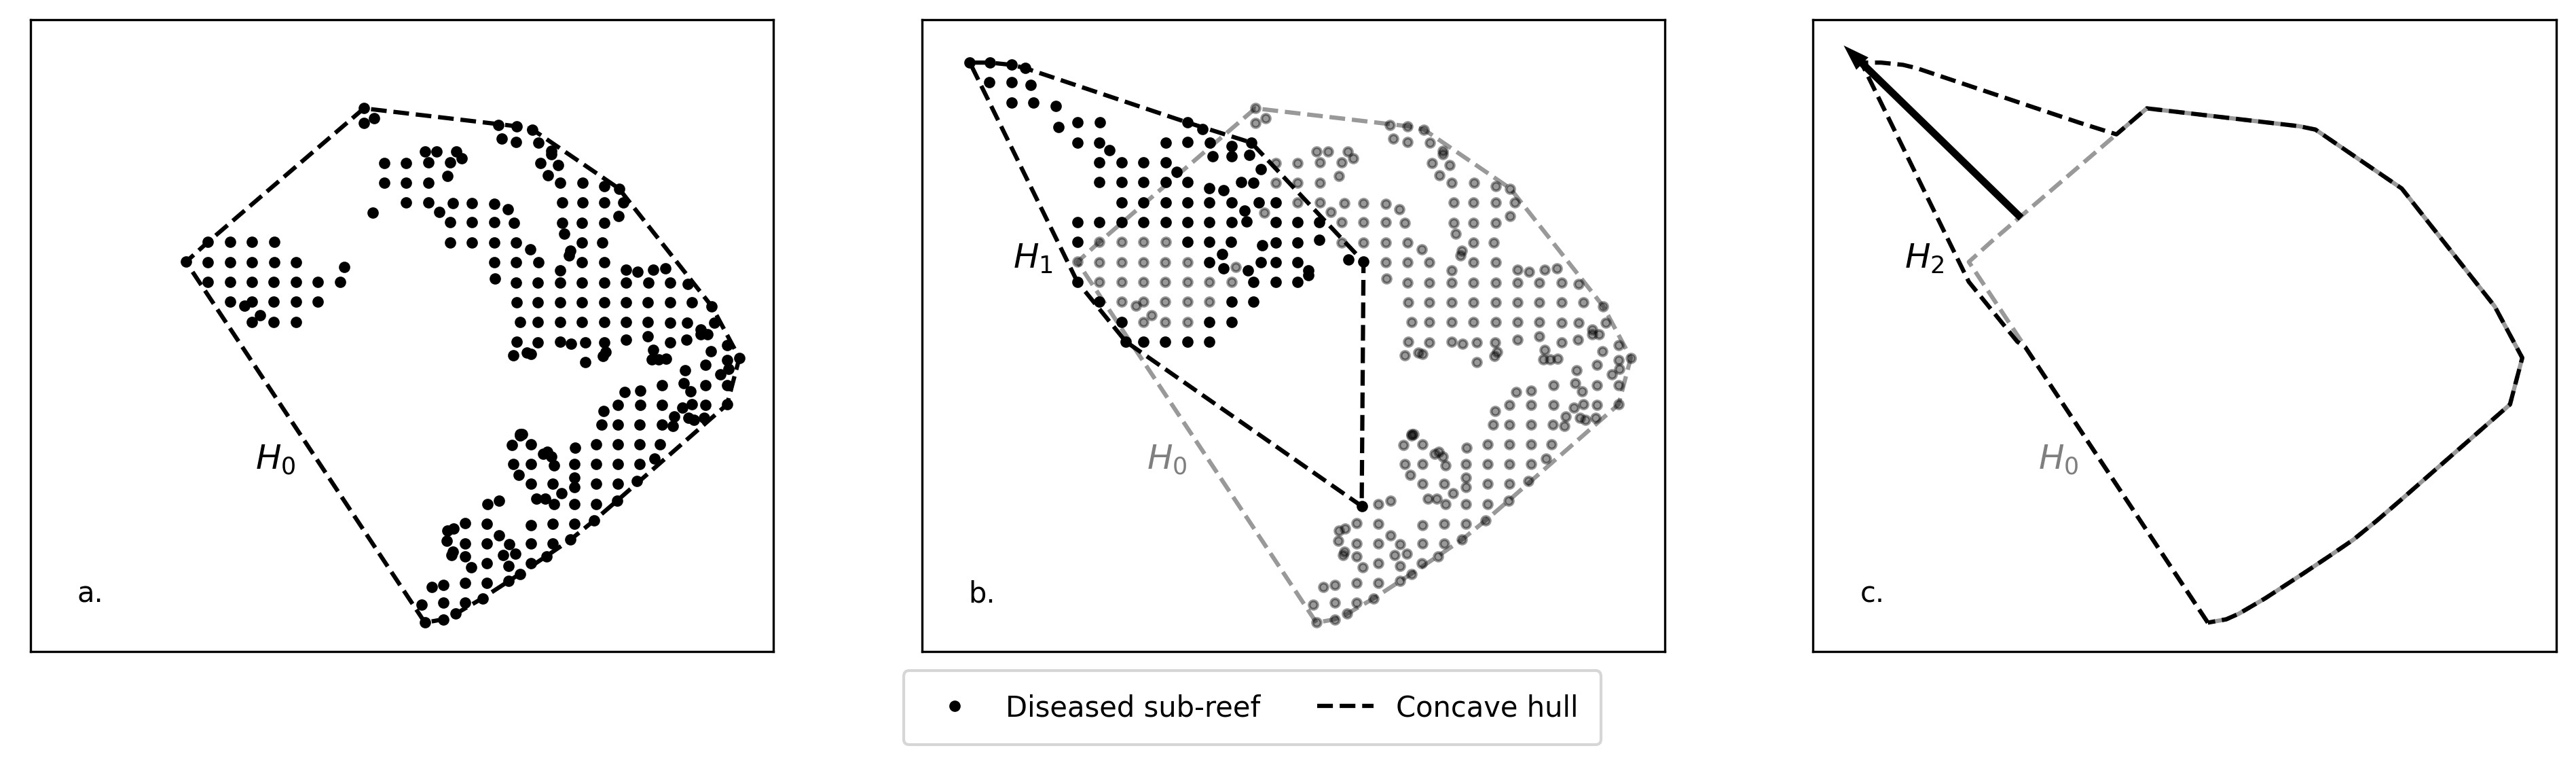
\includegraphics[width=.99\linewidth]{chapters/sctld/figures/hull_example_2.jpg}
    \caption{Method used to compute the disease front displacement during a simulated time interval.\textbf{a.} Concave hull $H_0$ of the diseased sub-reefs at the beginning of the simulated period. \textbf{b.} Concave hull $H_1$ of the sub-reefs diseased during the simulated time interval. \textbf{c.} Arrow showing the computed front displacement during simulated time interval between $H_0$ and $H_2$, the union of $H_0$ and $H_1$.}
    \label{fig:hull}
\end{figure}

\cite{muller2020spatial} estimated the speed of the spreading STCLD epidemics at around 92 m/day in the southern section of the FRT. In order to assess our simulation results in regard to this value, we developed a methodology to compute the displacement of the disease front during a given time interval within our simulated period. First, the concave hull $H_0$ of the diseased polygons at the beginning of the time interval was delineated. Then the concave hull $H_1$ of the polygons diseased during the time interval was computed while the concave hull $H_2$ was defined as the union of $H_0$ and $H_1$. This methodology is illustrated in Fig. \ref{fig:hull}. The distance traveled by the disease front was then obtained by computing the maximum distance between all pairs of points of $H_0$ and $H_2$. The epidemic's front speed was finally obtained by dividing the resulting distance by the number of days in the simulated time interval.

\subsection{Sensitivity analysis}
Disease agents and their vector were assumed to have a half-life of 30 days in the water column, governed by parameter $\gamma$ while inter- and intra-reef infection were assumed to occur at the same rate $\beta$. Although the sensitivity of our model to these two parameters was not extensively investigated in the present study, some additional simulations were performed to estimate how variations of their value might impact our results. To assess the influence of mass loss rate $\gamma$, additional connectivity matrices were computed using particles with a half-life of 15 days ($\gamma$ increased with a factor 2) in our dispersal model. Connectivity indicators were then computed for these matrices and their value was compared with the ones derived from 30-day-half-life connectivity matrices. Moreover, to evaluate whether the 'infectiousness' of disease agent might be reduced during its journey from reef to reef, epidemiological model simulations were performed with reduced inter-reef 'infection' rate $\beta=\frac{1}{2}\beta_0'$.

\subsection{Transmission experiments}\label{sec:transmission}
In parallel to this modeling study, laboratory-based transmission experiments of SCTLD were conducted by several independent groups for various end points including transmission dynamics and samples for molecular and histological analysis. Requests for transmission data were sent to members of the ‘Transmission’ sub-group of the Florida Disease Advisory Committee’s ‘Research’ working group as well as any other additional researchers that may have been conducting transmission studies on SCTLD. Data that was requested and subsequently provided included the location, dates, and duration of the experiment, the species used as the diseased colony (donor of disease agents) and apparently healthy colony (exposed to disease agents), the number of successful transmissions as well as the 'incubation' period following a contact with disease agents prior to disease signs. Additional information included the size of the colonies used in the experiment, the percent tissue loss of the diseased (donor) colony at the beginning of the experiment, and whether the apparently healthy (exposed) fragment was touching the diseased colony or not. 

The average probability of successful disease transmission was determined by taking the mean of the number of colonies exposed to the disease in each study divided by the total number of coral colonies exposed to diseased colonies. The ‘incubation’ period was identified as the average number of days after an apparently healthy coral colony was exposed to a diseased colony before visual disease signs occurred (i.e., active tissue loss). Only corals that eventually showed disease signs were integrated within the 'incubation' period calculation. 

Data were provided from 8 different research groups representing 15 institutions and 19 total collaborators providing a total of 109 data points. After amalgamating the contributed data, the mean probability of transmission of SCTLD to an apparently healthy coral had a likelihood of approximately $44.8 \pm 3.6$ \%. The probability of transmission ranged from 0 to 100\% depending on the experiment. Additionally, the time between exposure of an apparently healthy coral to a diseased coral and subsequently showing initial signs of tissue loss (i.e., 'incubation' period) was $9.7 \pm 1$ days.  

%%%%%%%%%%%%%%%%%%%
% --- RESULTS --- %
%%%%%%%%%%%%%%%%%%%
\section{Results}

\subsection{Exchanges of infected material}

Among the three modes of transport, bottom currents exhibited the lowest propagation range as they generated the networks with the smallest weighted connectivity length (Fig. \ref{fig:connect}). However, disease agents transported by bottom currents had the largest settlement success rate as these currents produced the graphs with the largest fraction exchanged. Therefore, bottom currents tend to transport more disease agents ro closer reefs compared to the two other modes of transport. Mean and surface currents, on the other hand showed similar spreading ranges with mean WCL of 20.63 km and 21.39 km respectively. However, the disease agents that surface currents transported had the lowest probability of settling successfully on reefs. Consequently, surface currents and bottom currents produced networks with similar mean out-degree, although surface currents have the potential to transport disease agents accross larger distances. Nonetheless, networks had larger median out-degree with bottom currents than with surface currents, which suggests that surface currents have a lower spreading potential than bottom currents. As a result of their large WCL and fraction exchanged, barotropic currents on the other hand exhibited the largest mean out-degree, which indicates that they have the strongest dispersal potential. 

Self-recruitment gives the fraction of disease agents settling on a reef that was produced on the same reef. The greater the self-recruitment value, the more the reef was isolated from the rest of the network. Since diseased material is less likely to settle on isolated reefs, self-recruitment informs on the potential for the disease to reach a given reef, whereas all three other indicators inform on the reef spreading potential. As mentioned before, self-recruitment is a relative measure and it might thus not give a complete picture of the amount of diseased material coming from upstream reefs that settles on a given reef. This is particularly true when considering reefs with different areas and coral cover. However, in the present study, we assumed a uniform coral cover and divided all the reefs into square sub-reefs with the same area. It is therefore reasonable to assume that sub-reefs with high self-recruitment act as weak sinks for diseased material. Fig. \ref{fig:connect} shows that the disease was more likely to settle on the reefs of networks generated by mean currents. This result is consistent with the values of the other connectivity measures, as reefs tended to be more strongly connected with mean currents. On the other hand, reefs were more isolated with bottom currents, as they produced the graphs with lowest WCL and out-degree. Finally, surface currents generated larger self-recruitment values than mean currents as they exhibited the lowest fraction exchanged. Therefore, although bottom currents exhibited stronger spreading potential than surface currents, reefs were more likely to become diseased with surface currents.

% \edit{Although the SCTLD has not reached the Marquesas yet in 2018, a preliminary analysis of the potential for disease transmission from the Florida Keys to the Dry Tortugas (where no sign of the SCTLD has been observed to date) can be performed based on the connectivity results of the present study (see appendix \ref{section:appendix}).}

\begin{figure}
    \centering
    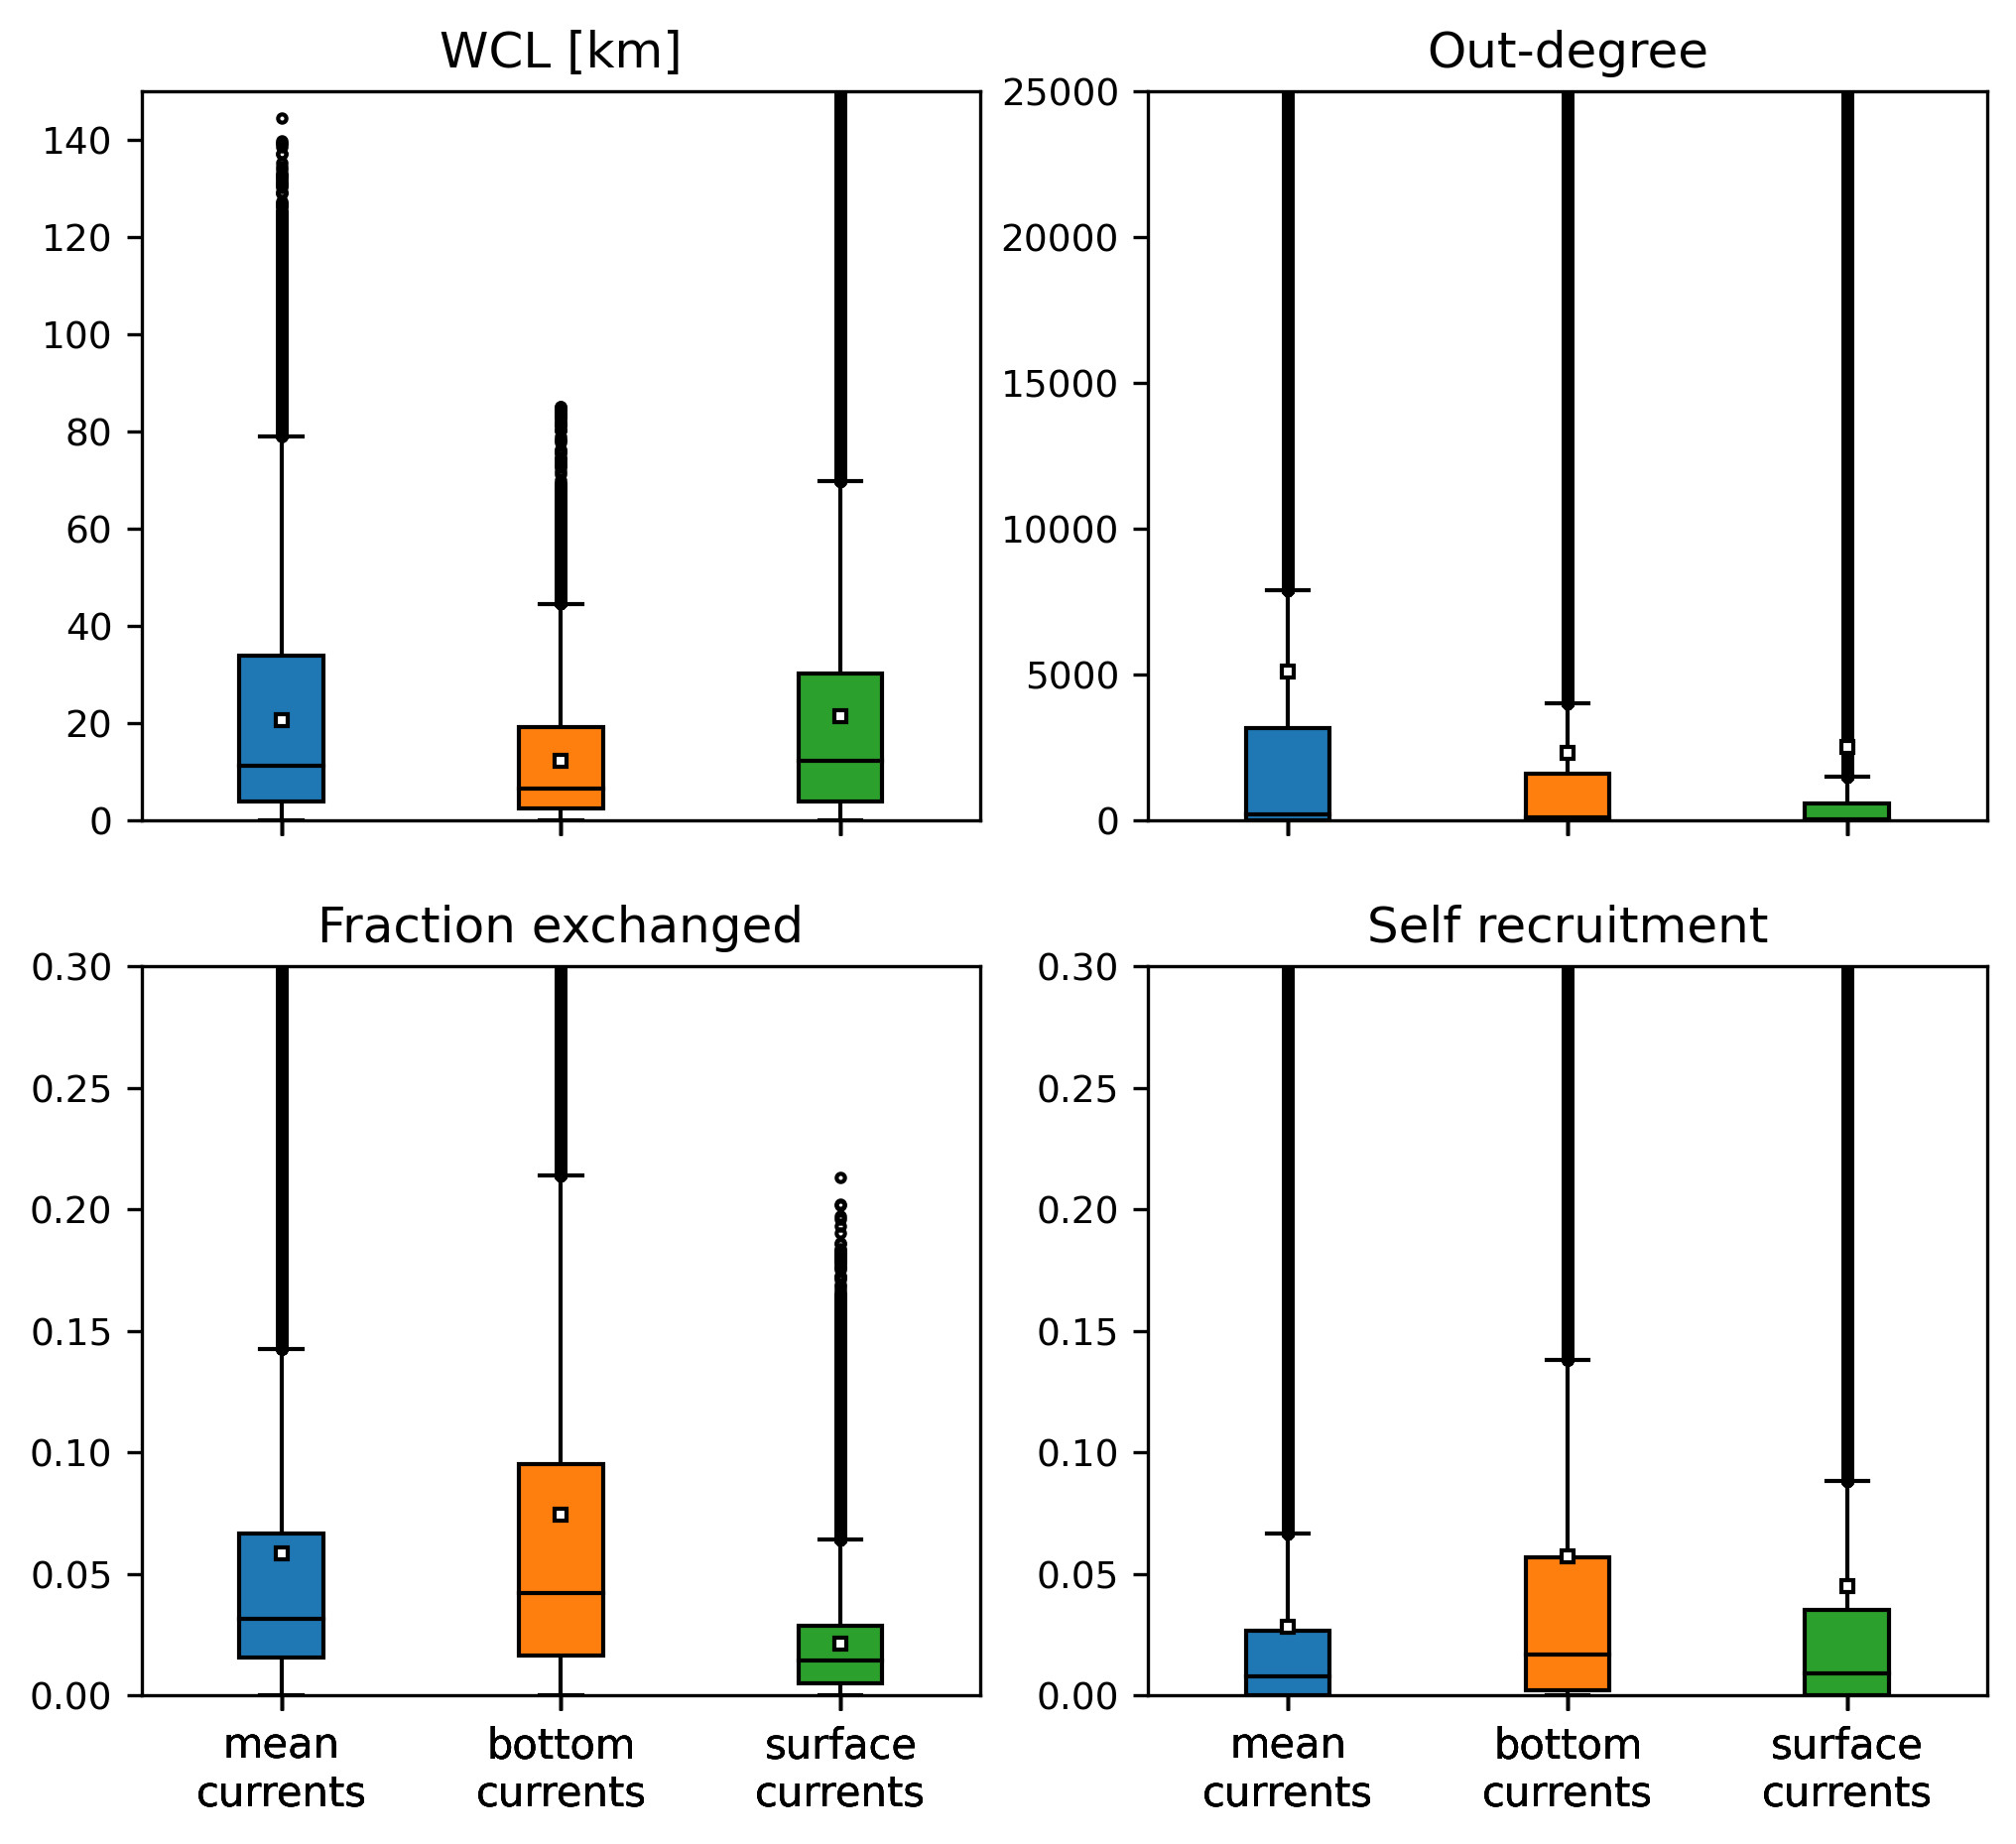
\includegraphics[width=.9\textwidth]{chapters/sctld/figures/connect_paper.jpg}
    \caption{Distribution of the indicators derived from the monthly connectivity matrices computed for each type of current during our simulated period. Mean values are indicated by white squares.}
    \label{fig:connect}
\end{figure}

\subsection{Epidemiological model results}

As aggregated observations showed a fraction of susceptible individuals of about $85\%$ after a year, a basic reproduction number $R_0=\beta'_0/\sigma=1.0345$ was found with Eq. \ref{eq:ratio}. Using this ratio, best fit to averaged disease prevalence observations was obtained with transmission rate $\beta_0'=\frac{1}{6.45}$ days$^{-1}$ and mortality rate $\sigma=\frac{1}{6.99}$ days$^{-1}$. Comparison of the evolution of the state described by Eqs \ref{eq:simplified} with observations is shown in Fig. \ref{fig:calibration}. Our model results accurately reproduced the observed fraction of susceptible individuals on colonies through time. However, the modeled fraction of removed individuals overestimated observations by about $5\%$. These discrepancies might be explained by the presence of "Unknown" values in our data sets as well as the simplifying assumptions of SIR models. Since 'infection' and removal occur at very close rates, the instantaneous fraction of diseased individuals on the reefs remained low through the outbreak, with a maximum value of about $0.4\%$.

\begin{figure}
    \centering
    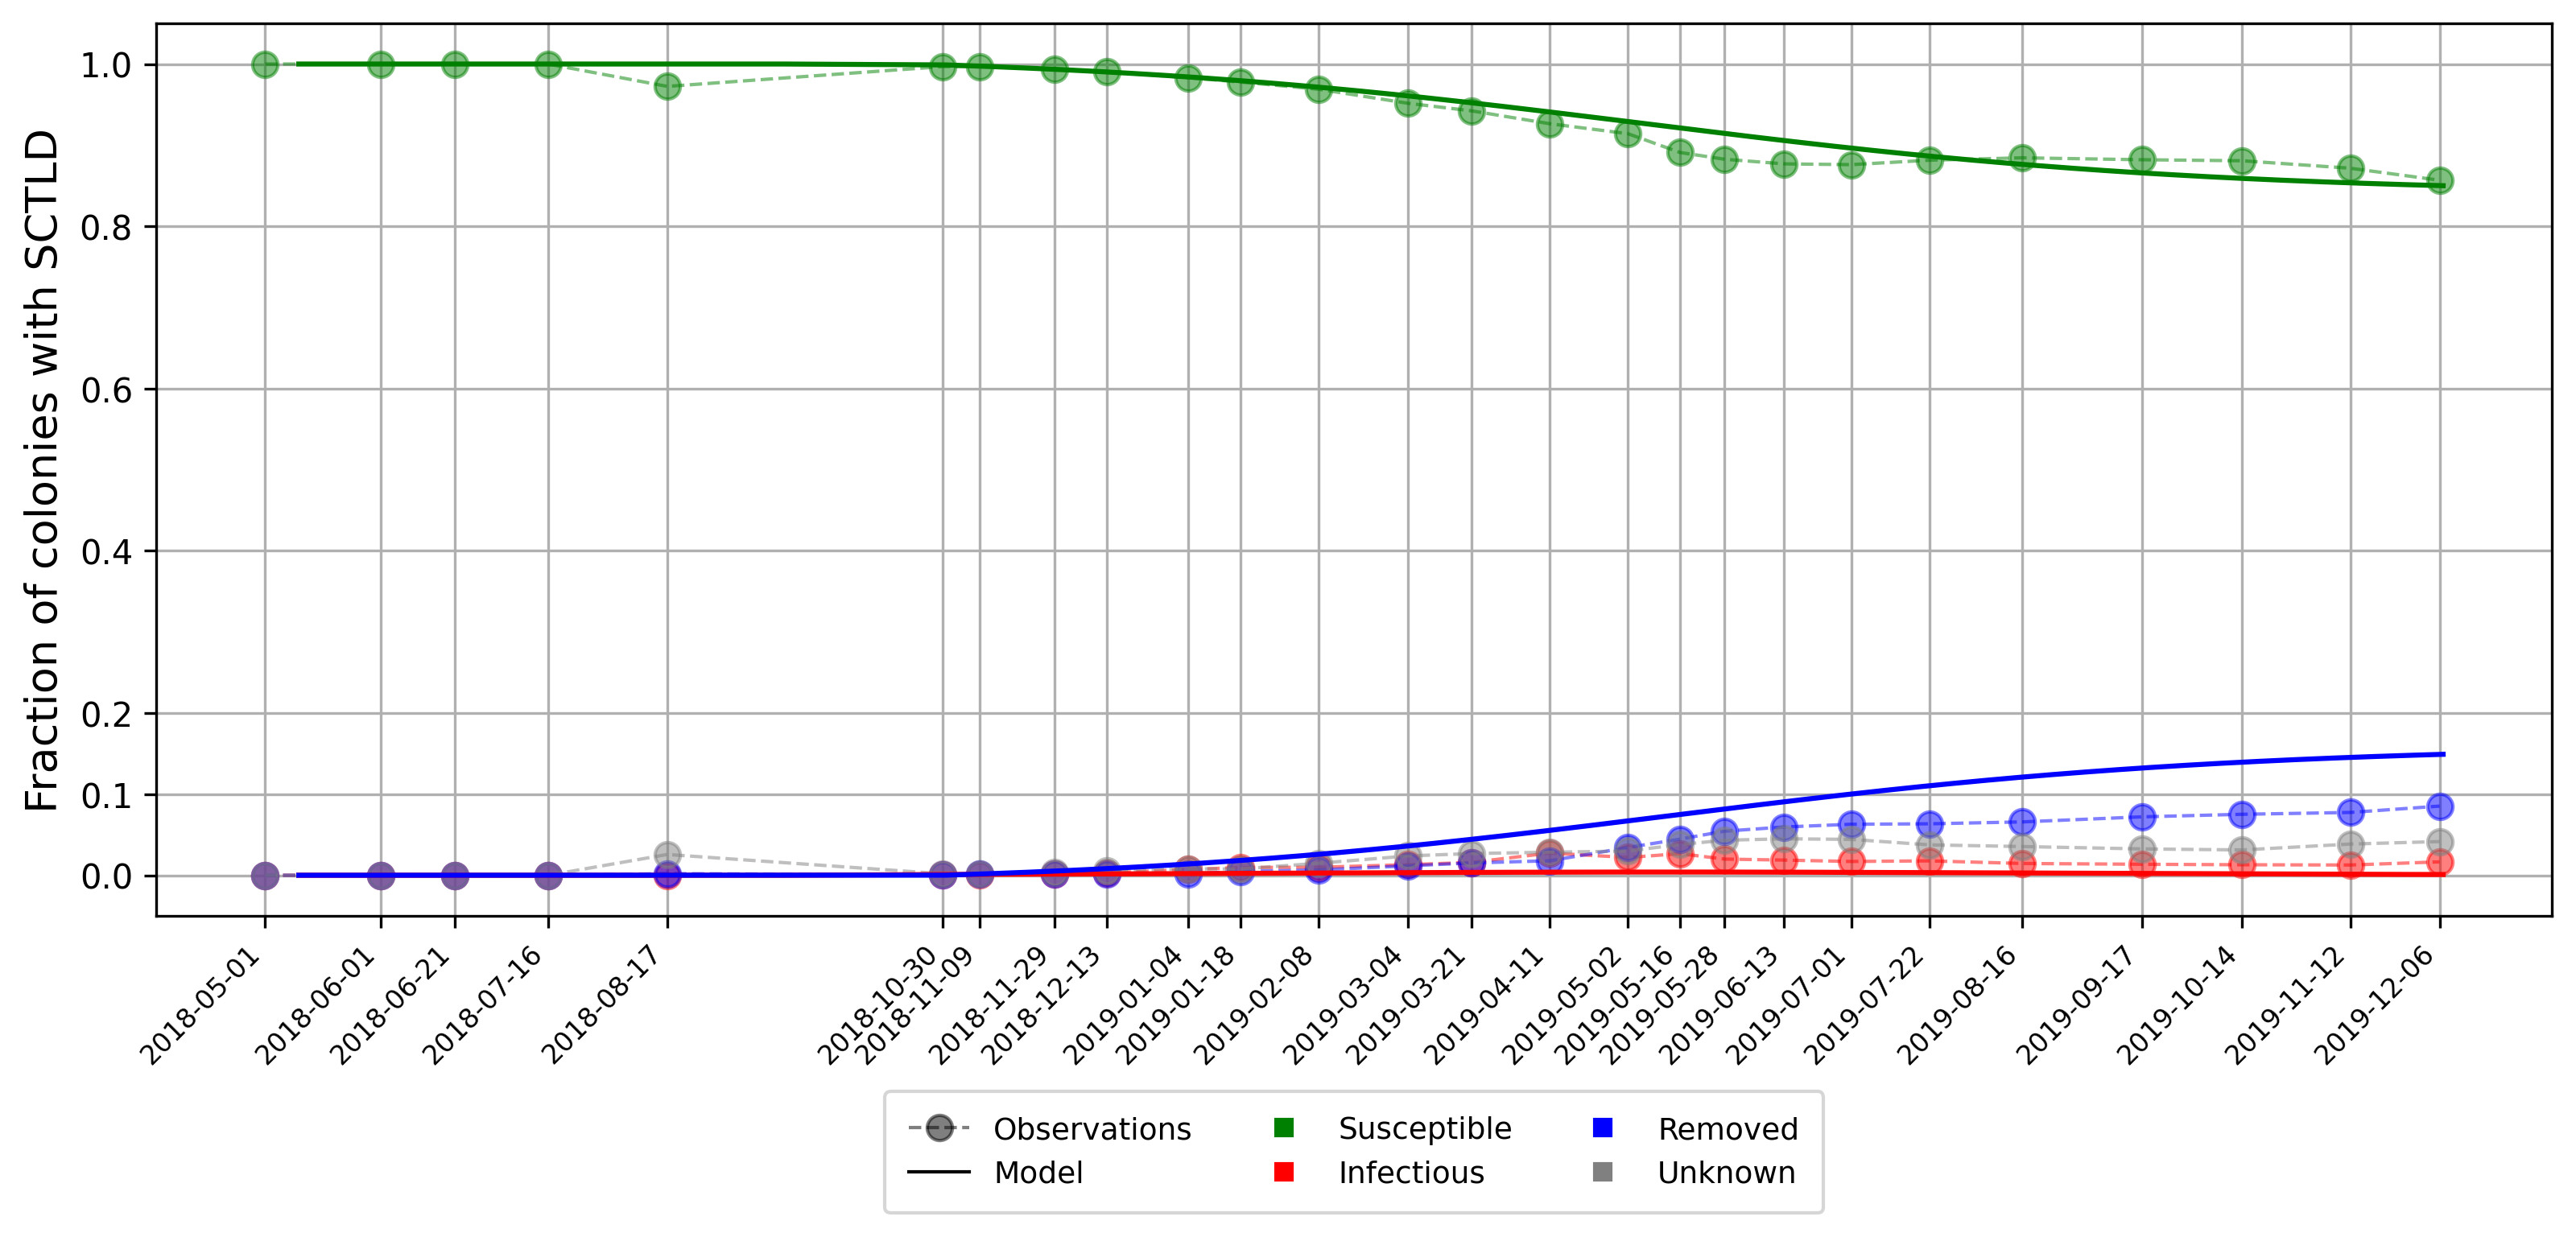
\includegraphics[width=.95\textwidth]{chapters/sctld/figures/sir_obs.jpg}
    \caption{Disease prevalence averaged over all monitored sites over time as modeled by Eqs. \ref{eq:simplified} using calibrated transmission and removal parameters $\beta_0'=\frac{1}{6.45}~\text{days}^{-1}$ and $\sigma=\frac{1}{6.99}$ days$^{-1}$.}
    \label{fig:calibration}
\end{figure}

Once the model was calibrated, epidemio-hydrodynamic model simulations were performed from 1st May 2018 to 1st April 2019 for each type of current and different values of the 'infection' threshold $I_0$. Two metrics were used to assess the accuracy of the model. First, the modeled front speed was compared to the reference rate of 92 m/day derived by \cite{muller2020spatial}. Furthermore, we computed the mean of the distances between each point where SCTLD had been observed during our simulated period (extracted from the 2018-2019 data sets described in section \ref{sec:init}) and the centroid of the closest reef polygon predicted to be diseased by our model during the same period (Fig. \ref{fig:results}). Bottom currents produced the slowest modeled disease propagation with a maximum front speed of $\sim 20$ m/day, while simulations performed with surface currents spread the disease at a maximum speed of about 60 m/day. However, surface currents tended to propagate the disease to the north, rather than westward, along the Florida Keys. This explains why bottom currents predict disease occurrence closer to field observations despite exhibiting slower front speed. Finally, mean barotropic currents outperform other types of current predictions regarding both criteria with a front speed of 107 m/day and a mean geographical accuracy of $\sim1.2$ km. This suggests that the disease agents of SCTLD may be transported within neutrally buoyant material driven from reef to reef inside the water column by mean currents.

Moreover, Fig. \ref{fig:results} shows a strong dependence of the model results to 'infection' threshold $I_0$, that gives the fraction of diseased individual that colonies can withstand before exponential disease growth is triggered on the reef. Front speeds of both mean and bottom currents reached a plateau for values of the threshold between $I_0=0.05\%$ and $I_0=0.1\%$, while the minimal prediction error was reached around $I_0 \approx 0.078\%$ with mean currents. For $I_0 > 0.1\%$, intra-reef 'infection' was strongly impeded and populations of 'infectious' individuals on diseased reefs were not able to become sufficiently large to infect other colonies on connected reefs. For values of $I_0$ lower than $0.05\%$ on the other hand, intra-reef 'infection' dominated and coral populations on diseased reefs were removed too fast to efficiently spread the disease through the network. Since disease propagation throughout the FRT only occurred for fairly small values of $I_0$ in our model, corals are expected to have low resistance to the causative agent of the SCTLD. 

\begin{figure}
    \centering
    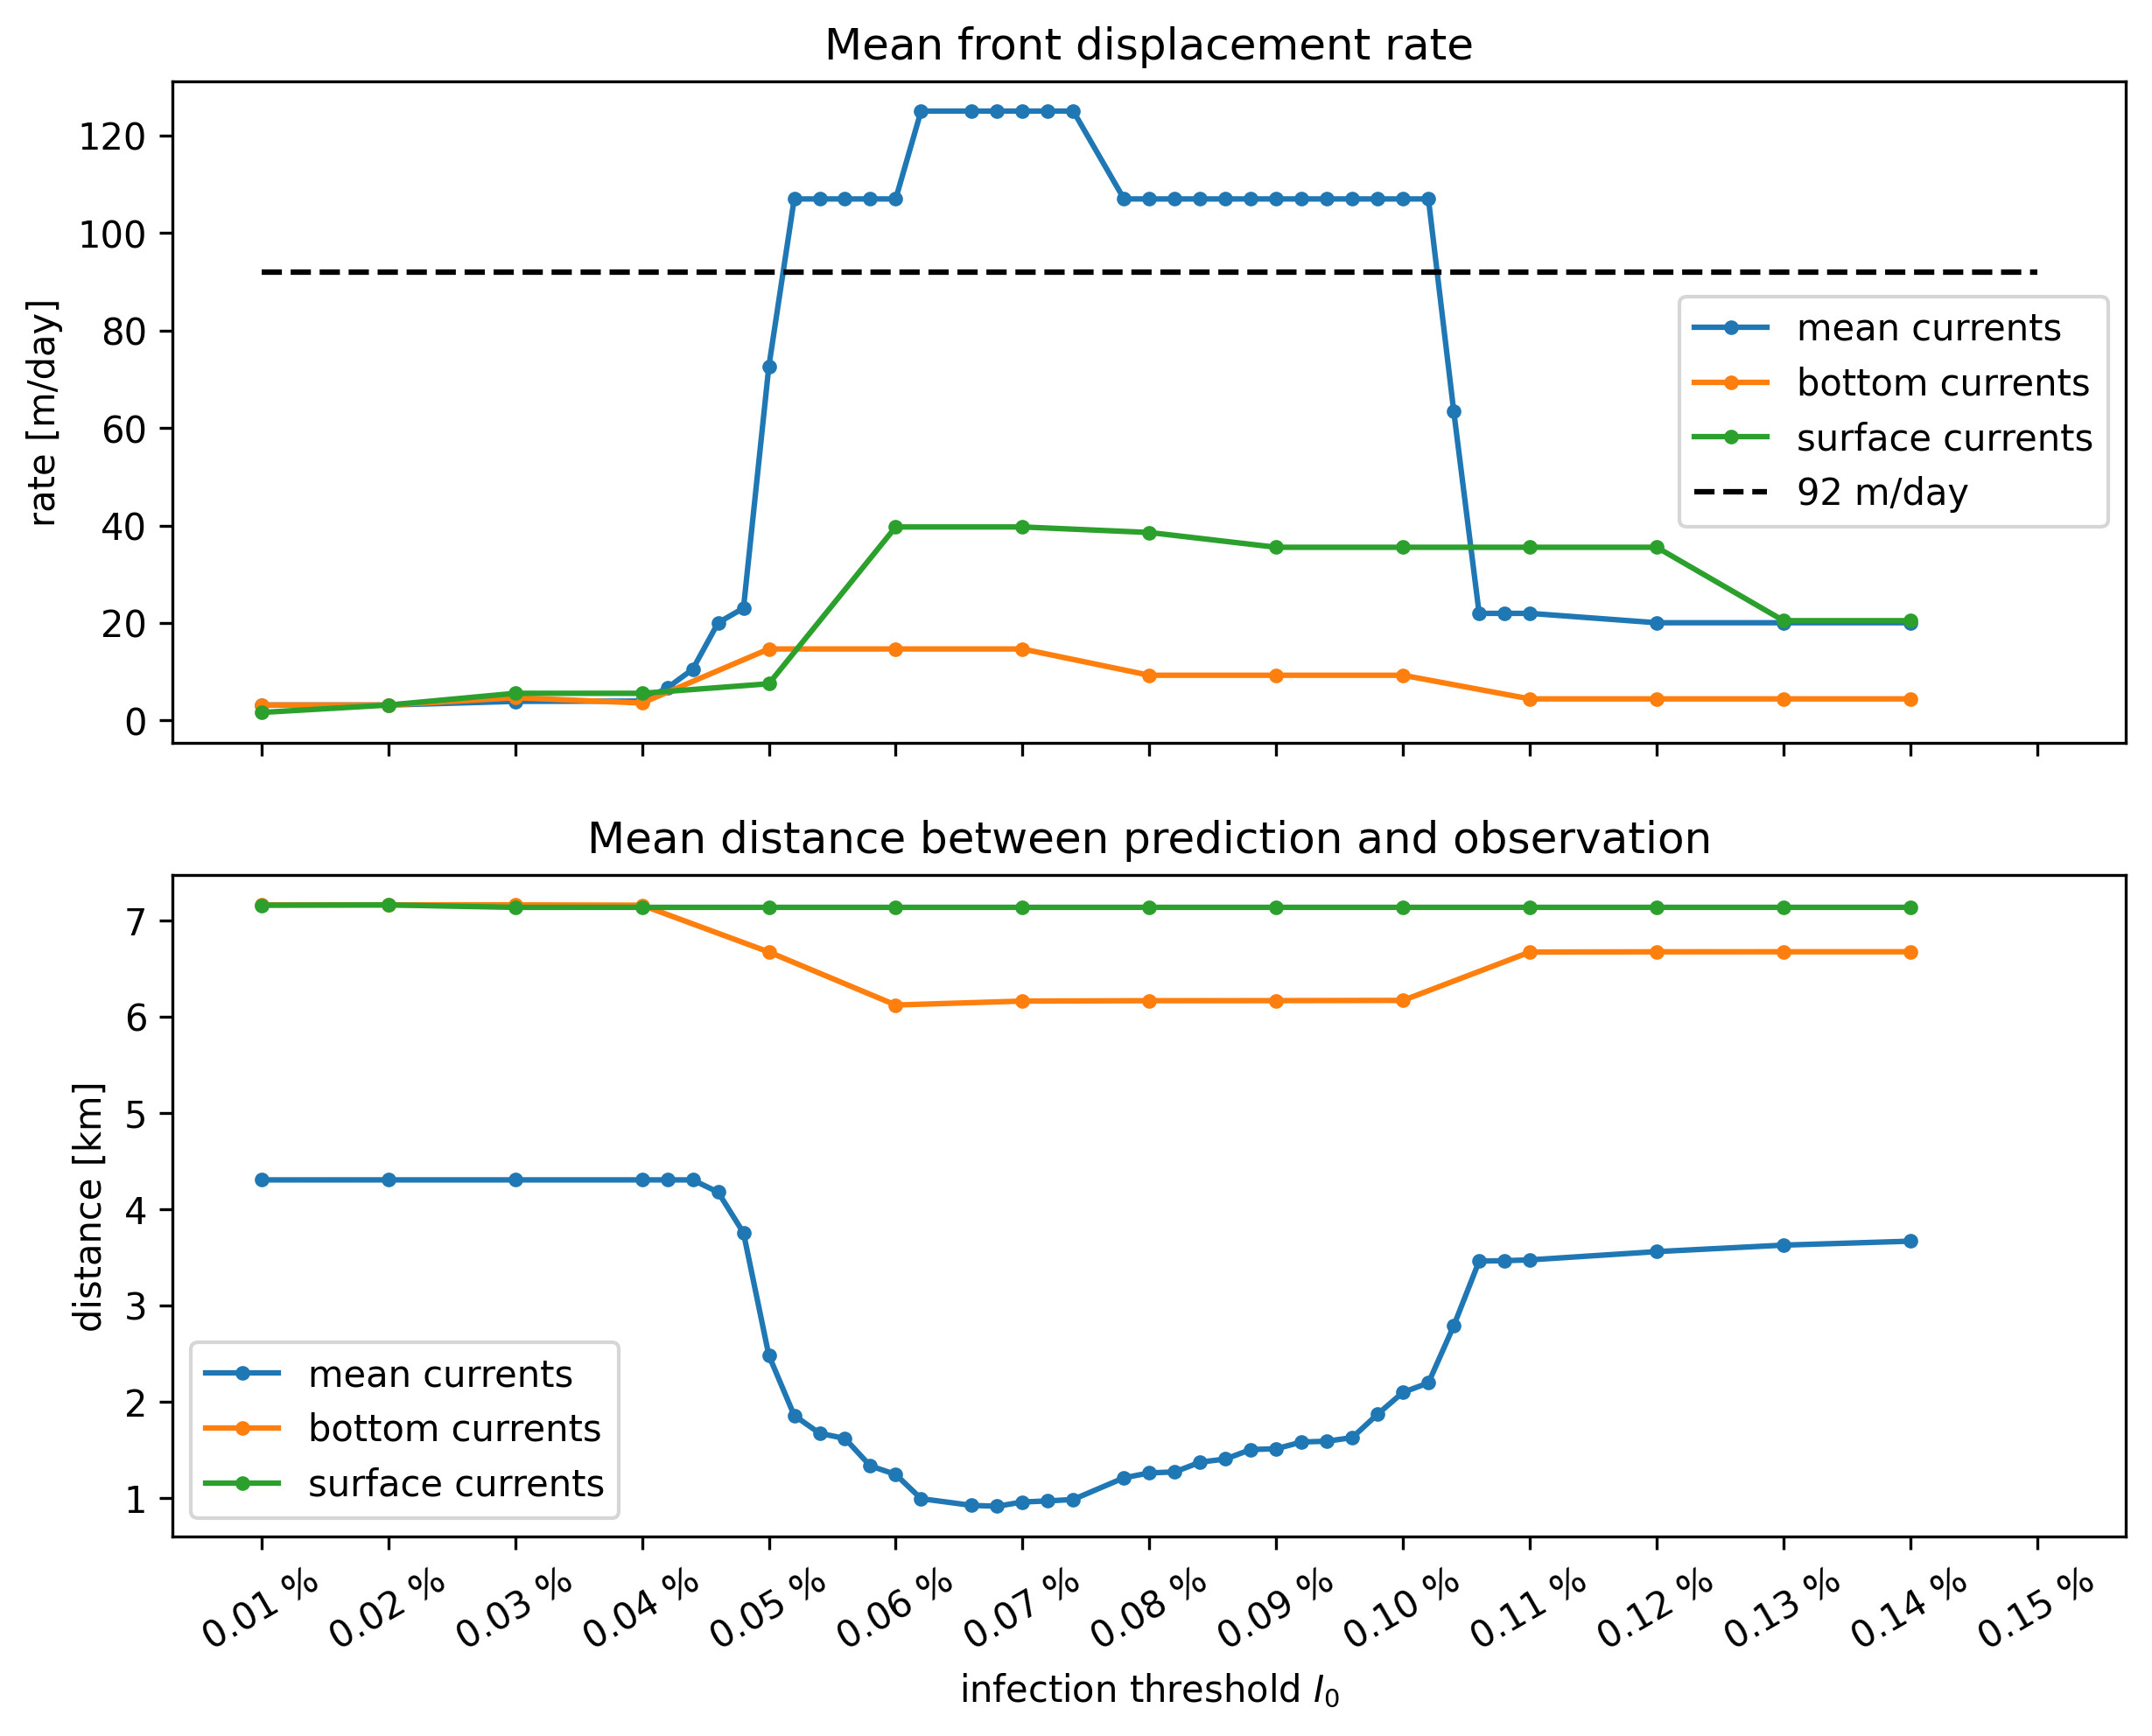
\includegraphics[width=.9\textwidth]{chapters/sctld/figures/sctld_validation_corrected.jpg}
    \caption{Summary of epidemiological model simulations with calibrated transmission parameters. \textbf{Top:} Modeled disease front speed for each type of current with respect to intra-reef 'infection' threshold $I_0$. \textbf{Bottom:} Mean distance between predicted diseased reefs and observed disease points. These results show that mean barotropic currents outperformed other modes of transport at reproducing the observed spread of the disease. The appearance of a plateau suggests that the modeled spread of the disease occurs for a well-defined range of values of $I_0$.}
    \label{fig:results}
\end{figure}

The results shown in Fig. \ref{fig:results} were obtained by removing the large reef located North to Vaca key, denoted Vaca reef in \cite{frys2020fine}, from our reef polygons. Preliminary simulations showed that this reef had close to no impact on the modeled spread of the disease to the rest of the FRT, as it sent very few disease agents to southerly and easterly neighboring reefs. Moreover, Vaca reef has a low coral coverage ($0-10\%$), which strongly impedes disease spread on the reef. However, as coral coverage was not taken into account in our epidemiological model, propagation of the disease on the reef was overestimated. This led to unrealistically strong modeled front speed variations due to the large size of the reef. Consequently, and in the absence of SCTLD observations on Vaca reef, this area was removed from our reef polygons in order to avoid overestimating the front speed.

% \begin{figure}
%     \centeringSubsection 1
%     \includegraphics[width=.9\textwidth]{figures/traj.png}
%     \caption{}
%     \label{fig:traj}
% \end{figure}

%\begin{figure}[h]
%    \centering
%    \includegraphics[width=.9\textwidth]{figures/hull_result.png}
%    \caption{Take home messages:\begin{itemize}
%        \item Our methods accurately captures disease front evolution through time (mtch between points and concave hulls)
%    \end{itemize}}
%    \label{fig:front}
%\end{figure}

\subsection{Sensitivity analysis}
Connectivity matrices computed using particles with a half-life of 15 days exhibited shorter range connectivity. However, the impact of increasing mass loss rate $\gamma$ in our dispersal model remained limited with variations in connectivity indicator values weaker than $10\%$. However, reducing inter-reef 'infection' rate $\beta$ by a factor 2 had a significant impact on epidemiological model outputs as predicted disease front speed did not exceed 20 m/day, far less than the observed speed of the disease front. This strong decrease can be explained by the interplay between inter- and intra-reef disease activity. Reducing inter-reef transmission rates decreases the fraction of diseased corals on reefs attained by disease agents, which in turn reduces the amount of disease agents sent to the rest of the network.


% === DISCUSSION === %
\section{Discussion and conclusions}

%% --- SUMMARY OF TAKE HOME MESSAGES --- %%

We developed an epidemio-hydrodynamic model to simulate the spread of the SCTLD throughout the entire FRT. Calibrating our model with colony-averaged prevalence observations, we estimated the species-averaged reproduction number $R_0$ to be slightly larger than one. Our model simulations suggest that barotropic currents best reproduce the observed spread of the disease among reefs in the lower Florida Keys. Bottom current did not spread disease agents far enough while surface currents did not allow disease agents to reside within the reefs long enough to ensure disease transmission that matched field observations. The results, therefore, suggest the causative agent of SCTLD is likely to be transported within neutrally buoyant particles in the water column. With this mode of transport, the propagation of the disease from reef to reef only occurred for a well-defined range of values of the 'infection' threshold $I_0$. This threshold is defined as the fraction of all sub-reef colonies that were diseased which triggered a rapid spread of the disease over the entire sub-reef area. Our results suggest that this occurred once $0.05-0.1\%$ of the colonies were diseased. These results suggest that, on average, corals appear to have a low resistance to SCTLD.

%% --- DISCUSSION OF TAKE HOME MESSAGES/MAIN RESULTS --- %%

% 1. MODEL PARAMETERS
After calibration, we estimated the species-averaged basic reproduction number $\beta_0'/\sigma$ to be equal to $1.0835$. This value, being close to 1, suggests modeled diseased individuals were removed from the system almost as fast as susceptible individuals became diseased. This situation caused the fraction of infectious corals on the reefs to remain fairly low (\ie $\leq 0.4\%$) through time. These results suggest that only a small fraction of the colonies caused the disease to spread on the reef during the outbreak. The observation-based species-averaged transmission period of 6.45 days used in the model was a reasonable estimation of the disease transmission dynamics, being of the same order of magnitude as the experimentally-derived mean incubation period of 9.7 days. The difference between the two values can be explained by field measurement uncertainties as well as the inability to perfectly mimic field conditions in laboratory. In the present study, the same values were used for inter- and intra-reef 'infection' rates $\beta$ and $\beta_0'$, \ie disease agents 'infectiousness' was assumed to remain unchanged during their journey from reef to reef. This assumption is consistent with sensitivity analysis results, which showed that reducing the value of $\beta$ strongly impeded disease propagation through the network. This outcome suggests that, to reproduce the observed spread, inter- and intra-reef transmission rates must have similar magnitude, \ie that the causative agent is not degraded while traveling from reef to reef. Given that the etiology of SCTLD is still unknown, the lack of degradation of the SCTLD causative agent over distances of tens of kilometers between reefs may help to narrow the search.

% 2. MEAN BAROTROPIC CURRENTS => NEUTRALLY BUOYANT VECTOR 

The fact that mean barotropic currents outperformed the other modes of transport can be explained by considering the trajectories of the particles used to model the transport of the disease causative agent. Due to the impact of winds on positively buoyant material, particles driven by surface currents are likely to be blown away from the reefs. Moreover, even when winds are pushing particles along the reef line, these particles spend less time over the same region than particles driven by mean and bottom currents. Smaller amounts of particle mass will therefore settle on reef polygons, leading to lower connection strengths in the potential connectivity matrix, \ie lower exchange of infectious material between reefs. Hence, despite being able to transport the disease over greater distances, surface currents are less efficient to drive the propagation of the disease. Particles driven by bottom currents, on the other hand, remain over the same region longer, producing larger entries of the potential connectivity matrix. Due to these large exchange probabilities between reefs, bottom currents are better at propagating the disease (Fig. \ref{fig:results}). Nevertheless, because bottom currents are slower, exchanges of disease agents occur within a more limited geographical range. Mean barotropic currents that carry particles greater distances while allowing for sufficiently large amounts of diseased material to settle on reef polygons, were thus best suited to propagate the disease at a speed similar to field-collected data (Fig. \ref{fig:results}).

Since mean currents were the only mode of transport that successfully reproduced the observed propagation speed of the disease in our model, the disease causative agent is expected to be transported within neutrally buoyant material inside the water column. Current-driven propagation seems reasonable as water-borne transmission is an important spreading mechanism for multiple coral diseases, including white band disease, white plague disease, white pox disease, white syndrome disease, \textit{Porites} ulcerative white spots diseases, and skeletal eroding band disease \citep{shore2019modes}. These results suggest that coral mucus or sloughed off diseased coral tissue may directly transmit SCTLD if they remain suspended within mean currents. \cite{aeby2019pathogenesis} showed that corals held within aquaria can transmit SCTLD to healthy colonies suggesting that these mechanisms may be occurring within reefs. Additionally, vectors such as zooplankton, phytoplankton, or even marine snow, may be transporting disease agents from reef to reef within the water column. \cite{landsberg2018} used histology to show an association between the location of the in hospite symbiotic algae that reside within the coral gastrovascular cavity and the area of tissue necrosis occurring within SCTLD-affected corals. These results have led to the working hypothesis that SCTLD could be associated with the symbiotic algae or the process of heterotrophic feeding and ingestion. The causative agent could also be transported within fine sediments such as silt, as suggested by \cite{rosales2020rhodobacterales}. Such sediments are easily eroded in shallow areas around coral reefs and would therefore be mostly transported inside the water column by mean barotropic currents. This hypothesis might be tested by adapting the deposition rate $\gamma$ used in our experiments to be consistent with the sedimentation rate of silt. However, such modification of $\gamma$ would alter the entries of our potential connectivity matrices. Nonetheless, sensitivity analysis of connectivity indicators suggest that such modifications would have a minor impact on model behavior and that the main results of this study would remain valid for larger deposition rates.

% 3. IMPACT OF I0/APPEARANCE OF PLATEAU
Coral resistance to SCTLD was represented by parameter $I_0$, defined as the maximum fraction of the colony that can become diseased without causing the disease to spread to the rest of the sub-reef site. The plateau shown in Fig. \ref{fig:results} highlights the impact of this parameter on the modeled propagation of the disease. On the one hand, when corals were strongly susceptible to the disease, diseased individuals were removed from the system too fast to become sustainable sources of disease agents in the network. On the other hand, if corals were weakly susceptible to the disease, very few corals became diseased and the disease barely propagated. Our simulations suggest that this value of resistance must be fairly low (around 0.07\%) in order to successfully spread the disease throughout the FRT. This seems to imply that susceptible coral species have very weak defense mechanisms against the causative agent of the disease.

%% --- LIMITATION AND POTENTIAL IMPROVEMENTS OF THE MODEL --- %%
% 1. Limitations of hydro
As with any modeling study, it is important to understand the assumptions on which the model is based. Here, we have used a 2D barotropic ocean model forced by the 3D model HYCOM \citep{chassignet2007hycom} in order to indirectly represent baroclinic phenomena. Such a model is well-suited to simulate the fate of neutrally-buoyant material in shallow regions. However, as depth-averaged currents do not accurately approximate the motion of particles in the bottom and surface layers, they have been modified to simulate the exchanges of negatively and positively buoyant material. In order to derive bottom and surface currents from mean barotropic currents, we used parameterizations consistent with both observations and theory \citep{ardhuin2009observation,perlin2007organization, kundu1976ekman, smith2009influence}. Although such parametric estimation of surface and bottom currents adds additional uncertainty to those simulations, using a 2D model as the basis for the study allowed for reef-scale resolution throughout the whole FRT with available computational resources. Such high-resolution allowed the simulation to explicitly represent recirculation eddies around islands and reefs, that significantly impact the weighted connectivity length as well as the local retention of pathogenic material on the reefs \citep{frys2020fine}.

% 2. Limitations of epidemiological model
The appearance of an interval of optimal values of threshold $I_0$ for the propagation of the disease in our results highlights the impact of coral resistance on the spread of SCTLD through the FRT. Therefore, a next step in our modeling approach would be further dividing coral populations of our polygons into highly susceptible (\eg \textit{Dichocoenia stokesii}, \textit{Meandrina meandrites}), intermediately susceptible (\eg \textit{Orbicella faveolata}, \textit{Montastrea cavernosa}), and weakly susceptible (\eg \textit{Acropora Palmata}, \textit{Acropora cervicornis}) sub-populations. The fractions of susceptible, infectious and removed individuals within these sub-populations would then be modeled with specific transmission ($\beta$, $\beta_0'$) and removal ($\sigma$) rates as well as specific infection thresholds $I_0$. Such approach would however require a detailed knowledge of the fine-scale distribution of the different coral species throughout the FRT. This knowledge about coral coverage could also be used to avoid overestimation of the front propagation, as in the case of Vaca reef.

%% --- NICE FINAL PARAGRAPH --- %%
Despite the limitations of its current formulation, our model brings unprecedented perspectives on the propagation mechanism of SCTLD throughout the FRT. Using a reef-scale spatial resolution, we determined the most probable mode of transport for the vector of the disease agent and deduced its host-species-averaged reproduction number based on prevalence observations. In addition, our model formulation provides a framework to quantify coral resistance to the disease.  This framework is a novel contribution to the study and modeling of marine diseases, as both inter- and intra-patch disease dynamics are modeled explicitly and realistically in time and space. As our model results are continuous through time, they can exhibit the variability of the propagation of SCTLD temporally and therefore bring additional insight into observation data. This study provides much-needed complementary insight into the identification of the causative agent of the SCTLD and the management of the crisis it generates. Furthermore, our modeling approach could be applied to other affected areas of the Caribbean, where there is still time to perform active management as the disease spreads throughout the region.

% === APPENDIX === %
% \appendix
% \section*{Appendix}
% 
% % --- MODEL FORMULATION --- %   
% \subsection*{Transmission data contributors}

% % --- MODEL EVALUATION --- %
% \subsection*{Subsection 2}

% \section*{Conflict of Interest Statement}
% The authors declare that the research was conducted in the absence of any commercial or financial relationships that could be construed as a potential conflict of interest.

% \section*{Author Contributions}
% TD developed the model, run the simulations and analyzed the results. EM, LG and EH conceptualized the study and designed the modeling experiments. EM collected the biological data. DH designed the epidemiological model. All authors contributed to the writing of the manuscript.
  
% \section*{Funding}
% This paper is a result of research funded by the Florida Department of Environmental Protection under award PO: B6A24 to Mote Marine Laboratory. 

% \section*{Acknowledgments}
% Computational resources were provided by the Consortium des \'Equipements de Calcul Intensif (\textsc{c\'eci}), funded by the \textsc{f.r.s.-fnrs} under Grant No. 2.5020.11. Thomas Dobbelaere is a PhD student supported by the Fund for Research training in Industry and Agriculture (\textsc{FRIA}/\textsc{FNRS}).

% Field data was collected at the permanent SWG sites were collected by Sara Williams, Cory Walter, Joe Kuehl, Ray Bannister, and Erich Bartels. These sites were funded from "Florida's State Wildlife Grant, FWC Agreement no. 16007".

% Contributors listed in Tab. \ref{tab:contributors} provided data to the transmission study.
% \begin{table}[h!]
%     \center
%     \begin{tabular}{|l|l|}
%         \hline
%         \textbf{Contributors: Transmission Data} & \textbf{Institutions} \\ \hline
%         Erinn Muller$^\ast$     & Mote Marine Laboratory                 \\ \hline
%         Katie Eaton$^\ast$      & Mote Marine Laboratory                 \\ \hline
%         Jan Landsburg           & Florida Fish and Wildlife              \\ \hline
%         Yasu Kiryu              & Florida Fish and Wildlife              \\ \hline
%         Esther Peters           & George Mason University                \\ \hline
%         Ray Banister            & Mote Marine Laboratory/Florida Tech    \\ \hline
%         Valerie Paul            & Smithsonian Marine Station             \\ \hline
%         Blake Ushijima$^\ast$   & Smithsonian Marine Station             \\ \hline
%         Nikki Traylor Knowles   & University of Miami                    \\ \hline
%         Michael Studivan$^\ast$ & University of Miami/NOAA AOML          \\ \hline
%         Joshua Voss             & Harbor Branch Oceanographic Institute  \\ \hline
%         Greta Aeby$^\ast$       & Qatar University                       \\ \hline
%         Marilyn Brandt$^\ast$   & University of the Virgin Islands       \\ \hline
%         Adrienne Corea          & Rice University                        \\ \hline
%         Laura Mydlarz           & University of Texas - Arlington        \\ \hline
%         Dan Holstein            & Louisiana State University             \\ \hline
%         Amy Apprill             & Woods Hole Oceanographic Institute     \\ \hline
%         Tyler Smith             & University of the Virgin Islands       \\ \hline
%         Sonora Meiling$^\ast$   & University of the Virgin Islands       \\ \hline
%     \end{tabular}
%     \caption{Data contributors to the transmission experiments described in section \ref{sec:transmission}, to which the calibrated model parameters were compared. Contributors highlighted with "$^\ast$" conducted the Data Sharing.}
%     \label{tab:contributors}
% \end{table}

% \section*{Supplementary Material}
% The Supplementary Material for this article is attached to the submitted document.

% === BIBLIOGRAPHY === %

%%% Make sure to upload the bib file along with the tex file and PDF
%%% Please see the test.bib file for some examples of references

% \appendix
% \section*{Appendix}
% \renewcommand{\thesection}{A}
% \setcounter{figure}{0}
% \renewcommand{\thefigure}{\thesection\arabic{figure}}
% \subsection{Connectivity between the Marquesas and the Dry Tortugas}\label{section:appendix}
% To assess the potential for disease transmission from the Marquesas to the Dry Tortugas, we computed the paths with the highest transmission probability between each possible pairing of a source reef in the Marquesas and a sink reef in the Dry Tortugas in our connectivity networks. To do so, a weight $w_{ij} = 1-C_{ij}$ was attributed to the edge between sub-reefs i and j, so that paths with lowest weight (i.e. shortest paths) in the network would correspond to connections with highest probability of exchange of disease agents. The shortest paths were then computed using the Python package python-igraph \citep{csardi2006igraph} for each monthly matrix obtained with barotropic currents, as they drive the modeled disease propagation that best matches observations (Fig. \ref{fig:results}).

% The most likely transmission pathways from the Marquesas to the Dry Tortugas are computed by taking the yearly average of the shortest paths obtained for each monthly connectivity (Fig. \ref{fig:appendix1}). Although the SCTLD has not reached the Marquesas yet in 2018, these preliminary results bring some insight into the exchange mechanisms between the Marquesas and the Dry Tortugas. First, the existence of multiple paths from the Marquesas to the Dry Tortugas suggests a possibility for disease agents produced in the Marquesas to reach the Dry Tortugas. Moreover, disease transmission seems more likely to originate from inshore reefs as paths starting from these reefs exhibit the largest exchange probability. Furthermore, the presence of indirect transmission pathways from the Marquesas to the Dry Tortugas suggests that reefs located between these two zones act as stepping stones that facilitate the propagation of the disease. This is particularly the case for disease agents produced in reefs located more offshore. Additionally, our results suggest a seasonal variation of these exchanges as no exchange from the Marquesas to the Dry Tortugas was modeled between September and November 2018 (Fig. \ref{fig:appendix2}). This absence of connection might be explained by the seasonal variation of the wind regime on the Western Florida Shelf. A non-seasonal influence which may have played a role is the offshore circulation associated with the Florida Current. The presence or absence of an oceanic mesoscale Tortugas gyre and associated frontal eddies has been shown \citep{lee1994evolution,lane2003mesoscale,sponaugle2005florida} to play an important role in connectivity patterns within the lower Keys, and between this region and the Dry Tortugas. Analysis based on operational ocean models from this period in 2018 (e.g., RTOFS, \cite{mehra2010real}) shows that the Tortugas Gyre was absent, with the Loop Current in a strongly retracted position - essentially, flowing straight from the Yucatan Channel into the Straits of Florida in November 2018; this may have significantly reduced connectivity during this period. The most likely period during which the infection could occur seems to be winter-early spring, so the presence or absence of this larger scale setup for later years may be important in understanding both disease and larval connectivity with the Dry Tortugas.

% \begin{figure}
%     \centering
%     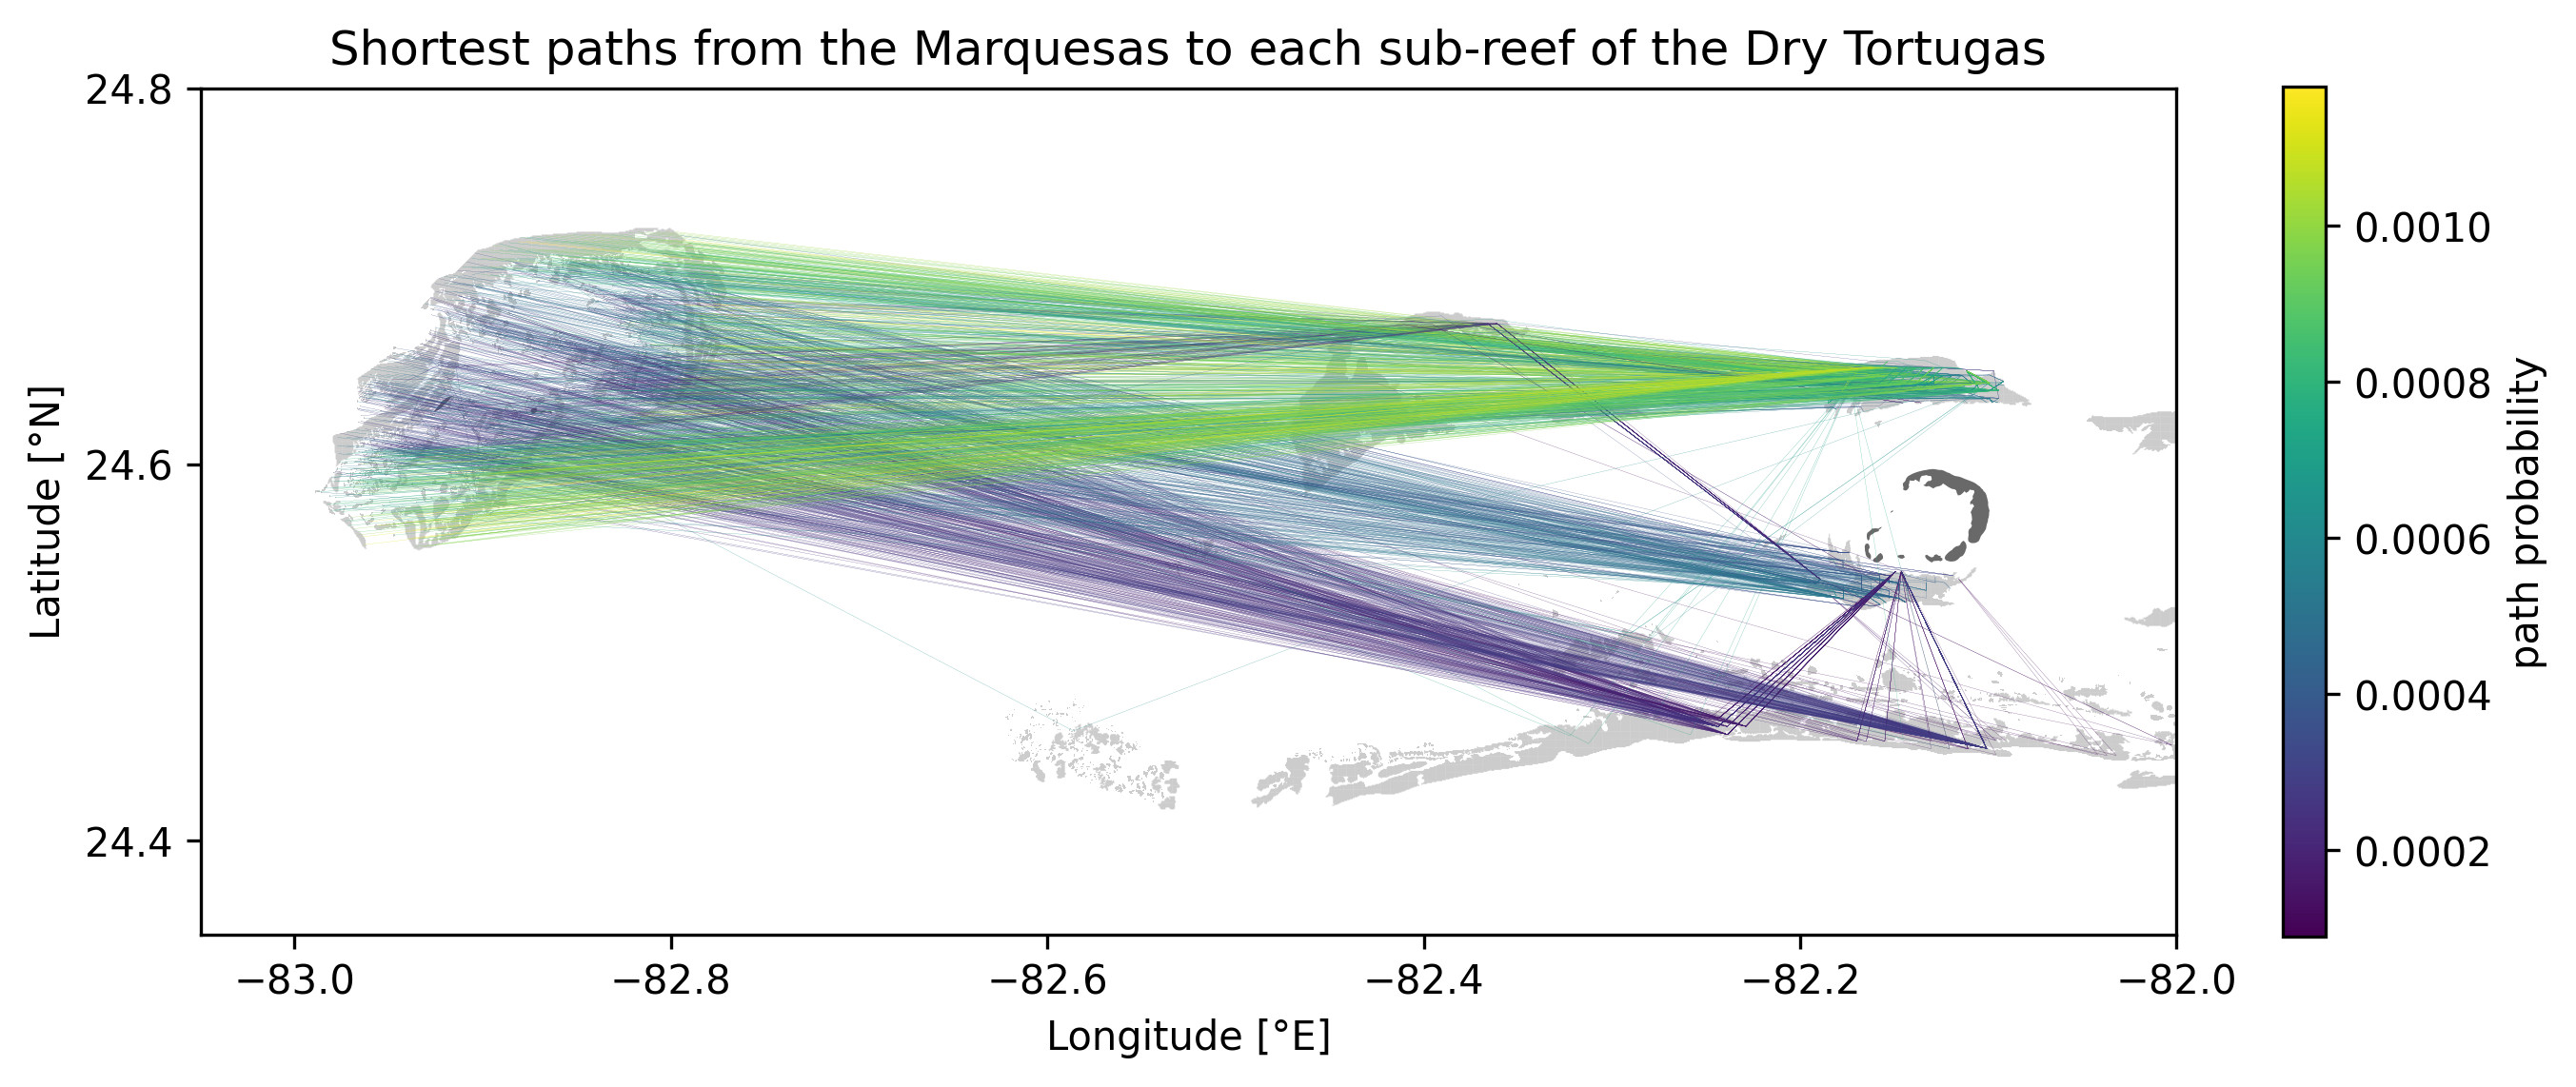
\includegraphics[width=.95\textwidth]{figures/paths_average.jpg}
%     \caption{Shortest paths to each sub-reef of the Dry Tortugas from the Marquesas computed from the yearly-averaged connectivity matrix obtained with mean barotropic currents. Reefs are  highlighted in light grey while islands are shown in dark grey.}
%     \label{fig:appendix1}
% \end{figure}

% \begin{figure}
%     \centering
%     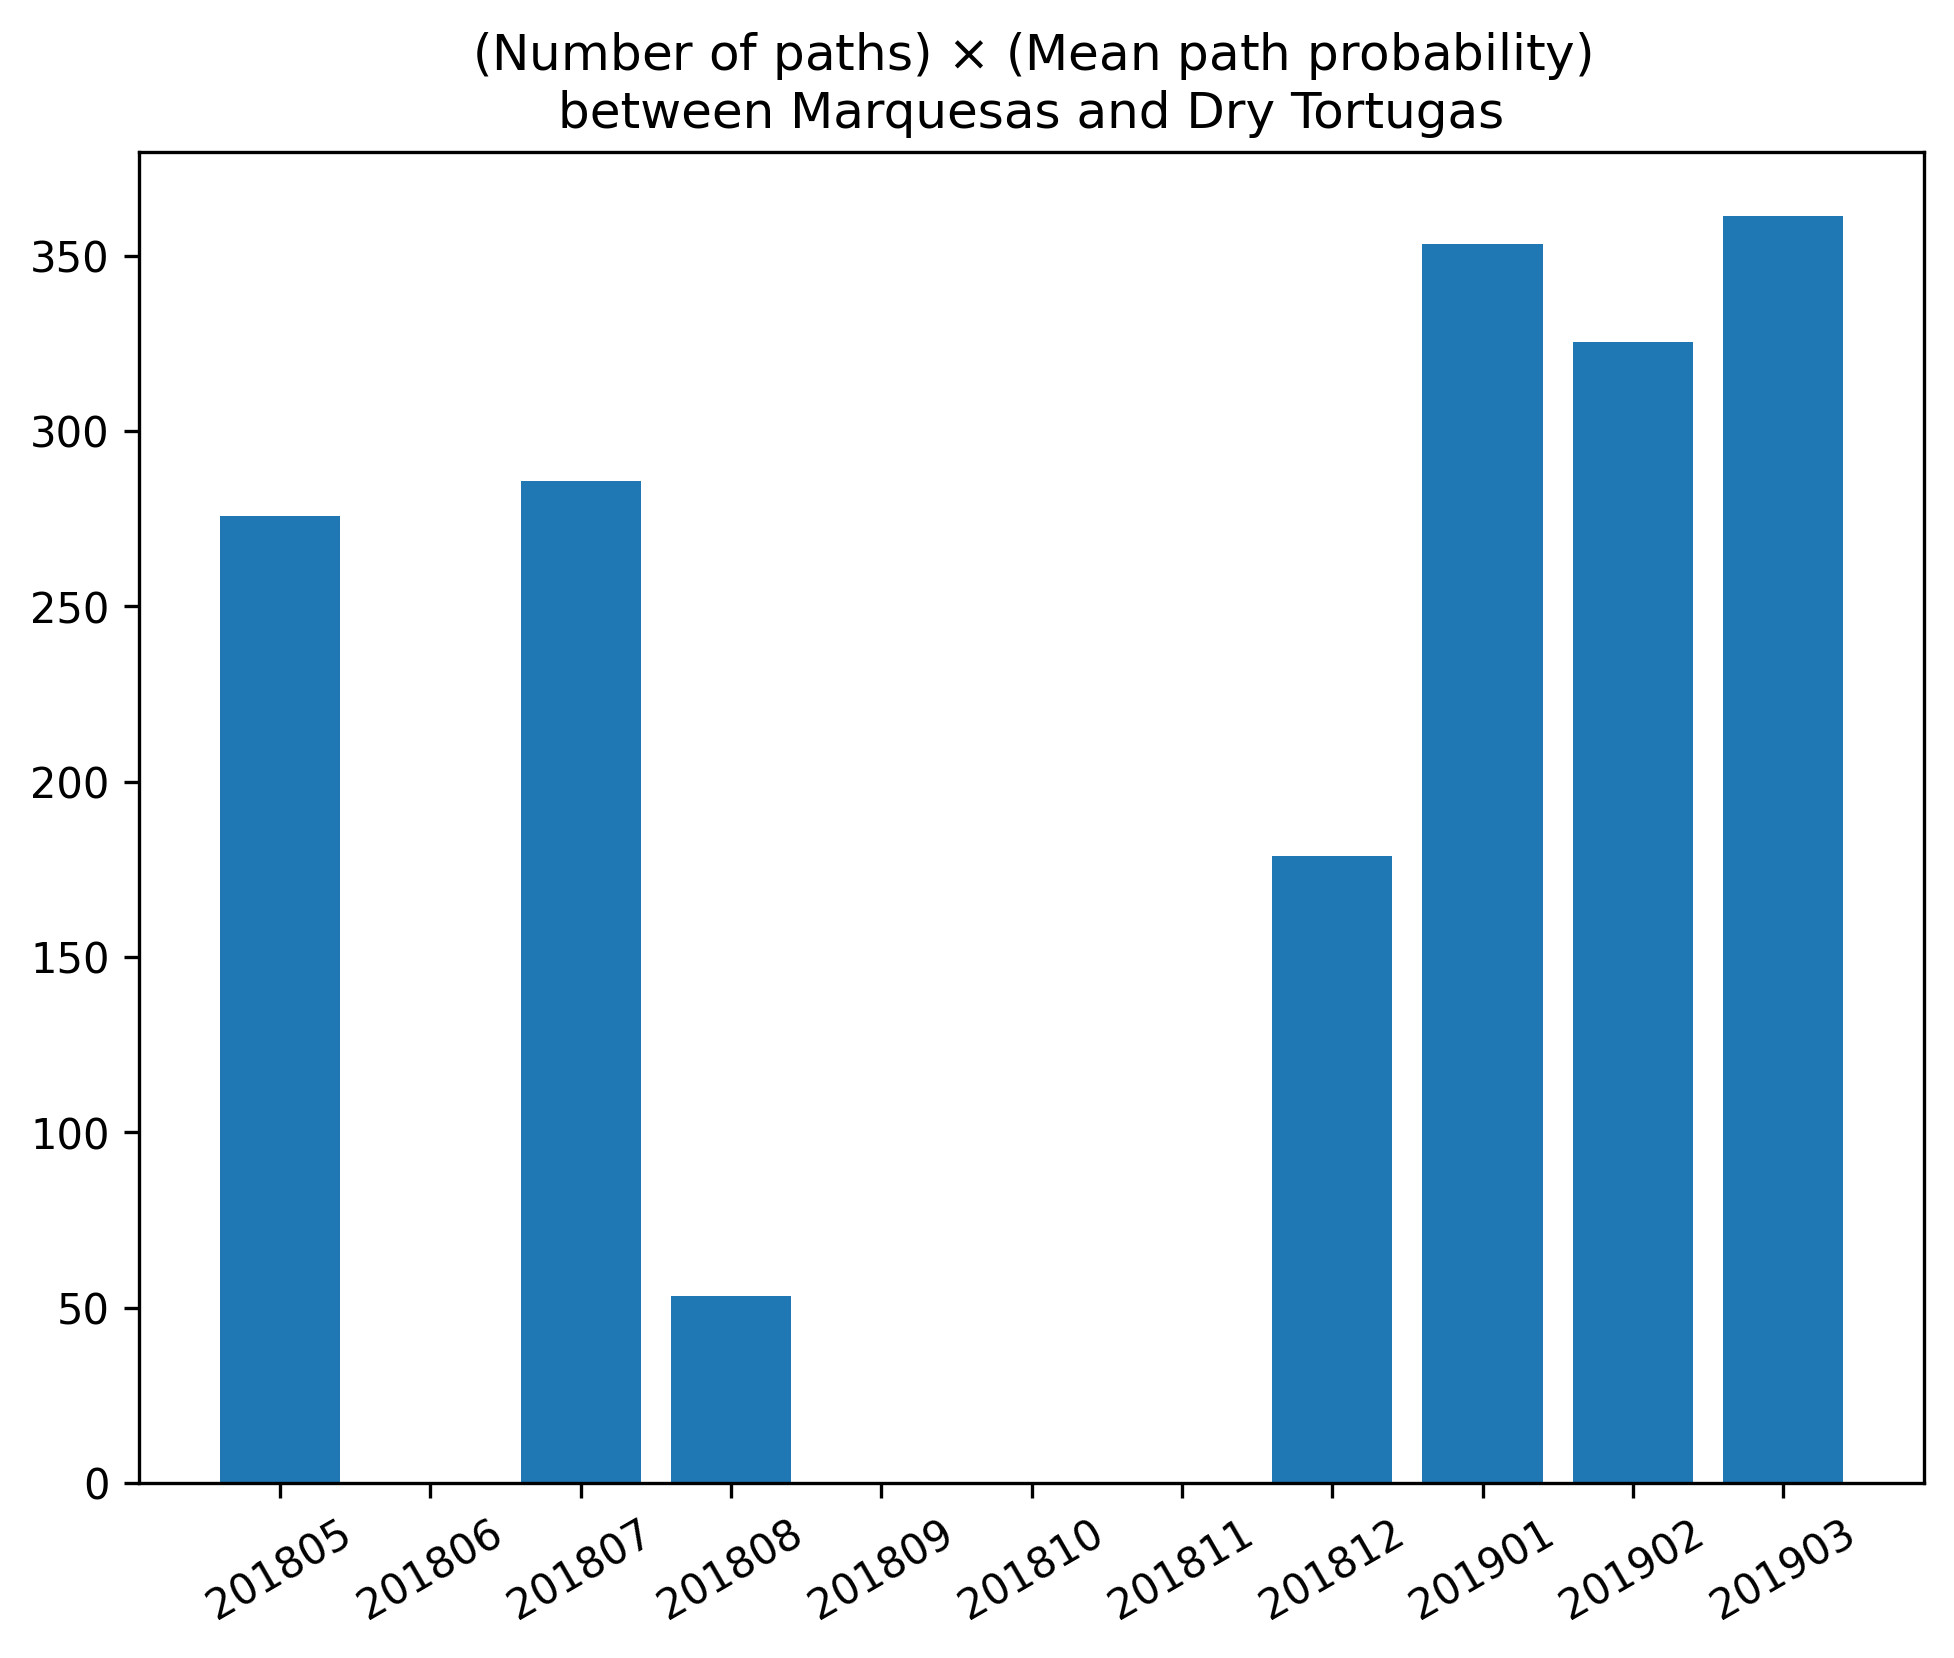
\includegraphics[width=.7\textwidth]{figures/time_series_MQ_DT_2.jpg}
%     \caption{Number of shortest paths from the Marquesas to the Dry Tortugas multiplied by their mean probability for each simulated month with barotropic currents.}
%     \label{fig:appendix2}
% \end{figure}
\mychapter{Transmission of SCTLD from the Marquesas to the Dry Tortugas}\label{chap:drto}
\chaptermark{Transmission of SCTLD from the Marquesas to the DRTO}  

This chapter is based on the following article:
\begin{list}{}{%
\setlength{\topsep}{0pt}%
\setlength{\leftmargin}{0.23in}%
\setlength{\listparindent}{-0.23in}%
\setlength{\itemindent}{-0.23in}%
\setlength{\parsep}{\parskip}%
}%

\item \textbf{Dobbelaere, T.}, Holstein, D. M., Muller, E. M., Gramer, L. J., McEachron L., Williams, S. D., \& Hanert, E. (2022). Connecting the dots: Transmission of stony coral tissue loss disease from the Marquesas to the Dry Tortugas. \textit{Frontiers in Marine Science}, 9. \href{https://www.frontiersin.org/article/10.3389/fmars.2022.778938}{doi: 10.3389/fmars.2022.778938}.

\end{list}

\begin{abstract}
    For the last seven years, Florida's Coral Reef (FCR) has suffered from widespread and severe coral loss caused by the stony coral tissue loss disease (SCTLD). First observed off the coast of Miami-Dade county in 2014, the outbreak has since spread throughout the entirety of FCR and some areas of  the Caribbean. However, the propagation of the disease through FCR seemed to slow down when it reached the western end of the Marquesas in August 2020. Despite being present about 30 km ($\sim$20 miles) from the Dry Tortugas (DRTO), SCTLD was not reported in this area before May 2021. As SCTLD transmission is likely to be waterborne, here we suggest that this apparently delayed propagation is related to eddy activity near the DRTO under the influence of the Loop Current/Florida Current system. To quantify the impact of the local ocean circulation on the spread of SCTLD from the Marquesas and the DRTO, we evaluated the hydrodynamic-predicted connectivity between these two regions using a high-resolution hydro-epidemiological model between May 2018 and May 2021. Our results suggest that the Marquesas and the DRTO were not connected during February-October 2020 and January-May 2021. These periods coincided with either the occurrence of Tortugas gyres and mean circulation with an eastward component between the Marquesas and the DRTO or the presence of southward currents. Our results suggest that disease agents probably reached the DRTO in November 2020 and that they most likely originated from southern or northwestern reefs of the Marquesas. This study provides novel insight into the role played by the hydrodynamics in the spread of SCTLD within the western-most edge of FCR, and in propagating the disease to uninfected locations.
\end{abstract}

%\newpage



\section{Introduction}
Over the last seven years, Florida's Coral Reef (FCR) has suffered from a widespread decline in living, reef-building corals due to a multi-year coral-disease outbreak \citep{precht2016unprecedented,walton2018impacts}, called stony coral tissue loss disease (SCTLD). First reported off the coast of Miami-Dade county in 2014, the disease has since spread through the entirety of FCR as well as other sites within the Caribbean \citep{alvarez2019rapid,kramer2019map,estrada2020reef} and affected more than 20 scleractinian coral species \citep{noaa2018}. The range of species affected coupled with the large spatial and temporal extents of the outbreak make SCTLD the most severe disease outbreak to have affected coral reefs on record.

Previous study of the spatio-temporal dynamics of SCTLD between West Palm Beach and Marathon showed that the epizootic propagated at a rate of $\sim$100 m/day to the north and $\sim$92 m/day to the south, hitting the Middle Florida Keys in 2017 \citep{muller2020spatial}. The disease was then reported in the Lower Keys in summer 2018 \citep{frrp2018}; near Key West in winter 2018 \citep{frrp2018}; on the easternmost boundary of the Marquesas subregion in October 2019 \citep{frrp2019}; and at its western end, approximately 11 km. west of halfmoon shoal, in August 2020 \citep{frrp2020}. SCTLD was observed propagating faster than 100 m/day within the Marquesas between October 2019 and August 2020 and would have reached the reefs of the Dry Tortugas (DRTO) by February 2021 if it had spread at a similarly high propagation rate \citep{kramer2019map}. These propagation rates were observed in a relatively dense shallow-water reef system and mostly occurred through transmission from neighbor to neighbor. Disease agents then had to cross 30 km ($\sim$20 miles) of open waters to reach the reefs of the DRTO. The disease was ultimately observed in May 2021 \citep{kramer2019map} in the southeast of the DRTO. To date, questions remain about the timing of the spread of the disease to the DRTO as well as the role played by hydrodynamics in the process.

The DRTO coral reefs are among the most preserved, but also vulnerable, marine ecosystems of the continental United States \citep{kourafalou2018physical}. They are part of the Florida Keys National Marine Sanctuary (FKNMS), under the jurisdiction of the Tortugas Ecological Reserve that covers around 566 km$^2$ of no-take marine reserves \citep{ault2006building}. Since the establishment of DRTO in July 2001, fish populations within the managed areas have significantly increased in size, adult abundance, and occupancy rates, therefore favoring the establishment of sustainable fisheries \citep{ault2013assessing}. Furthermore, because of their location and hydrodynamics, DRTO reefs are believed to be important sources of recruitment for coral-reef fishes downstream in the Florida Keys \citep{domeier2004potential} and thus significantly contribute to the overall resilience of the Florida Keys coral-reef ecosystem.

Although the pathogen responsible for the disease remains unknown to date, hydrodynamics are likely to play an important role in its propagation. Modeling studies suggest that the observed spread of the disease can be reproduced by simulating the dispersal of neutrally buoyant particles \citep{dobbelaere2020coupled}, while ex situ experiments show evidence of waterborne disease transmission \citep{aeby2019pathogenesis, eaton2021measuring,meiling2021variable}. Accounting for the underlying ocean circulation is therefore important to understand the evolution of the propagation of the disease. The observed apparent stalling of the spread of SCTLD from the Marquesas to DRTO reefs may be explained by ephemeral or persistent oceanographic features in the area that initially prevented the transmission of disease agents further west.

The ocean circulation between the Marquesas and the DRTO is strongly driven by the Loop Current (LC). This ocean current brings warm waters from the Caribbean Sea through the Yucatan Channel, loops anti-cyclonically through the northeastern Gulf of Mexico (GoM) and finally exits through the southern Straits of Florida, where it forms the Florida Current (FC). The northward penetration of the LC through the GoM varies throughout the year, and sporadically an anticyclonic ring separates from the current \citep{leipper1970sequence, maul1977annual,vukovich1988loop}. The dominant mesoscale feature near the DRTO is the formation of quasi-stationary eddies with a diameter of 100-200 km \citep{lee1994evolution,fratantoni1998influence}, usually called Tortugas gyres or eddies. \cite{fratantoni1998influence} hypothesized that the formation of these eddies as well as their lifespan was linked to the generation of anticyclonic rings from the LC in the GoM, while \cite{kourafalou2012florida} showed the relation between eddy formation dynamics near the DRTO and meandering of the FC. These eddies can remain up to 120 days near the DRTO before moving eastward at a speed of 5 km/day under the action of LC frontal eddies \citep{maul1977annual}. Tortugas gyres have been identified as an important mechanism for the potential retention of larvae of invertebrates and fishes on the southwest Florida shelf \citep{lee1994evolution, sponaugle2005florida, kourafalou2012florida} and might therefore have impacted the dispersal of disease agents from the Marquesas to the DRTO.

The objective of the present study was to apply the same modeling tools as \cite{dobbelaere2020coupled} to determine the potential impact of the circulation in the GoM on the delayed propagation of SCTLD between the Marquesas and the DRTO. This was performed by evaluating the evolution of the hydrodynamic-predicted connectivity between these two regions between May 2018 and May 2021. We then assessed how large-scale ocean circulation features, such as Tortugas gyres, could have prevented the transport of potential disease agents from the Marquesas to the DRTO. Ultimately, this study aims to provide novel insight on the role hydrodynamics have played in the spread of SCTLD throughout the western-most area of FCR, which further informs how it has, and will continue to, spread throughout the tropical western Atlantic

% === METHODS === %
\section{Methods}
Stony Coral Tissue Loss Disease data was obtained by using the Florida Reef Resilience Program's Disturbance Response Monitoring Report for 2019 and 2020 \citep{frrp2019,frrp2020} as well as the Atlantic and Gulf Rapid Reef Assessment (AGGRA) resources for SCTLD reported throughout the Caribbean, an open access spatial and temporal database curated by experts in Caribbean coral reef ecology \citep{kramer2019map}. Assumptions associated with SCTLD included the following: $(i)$ SCTLD is different from other tissue loss diseases previously reported on corals (i.e. white plague, white syndrome) based on its ecology and case definition \citep{noaa2018}, $(ii)$ SCTLD is transmitted, in part, by ocean currents \citep{aeby2019pathogenesis, muller2020spatial,eaton2021measuring} and $(iii)$ SCTLD was along the western most reef area of the Lower Florida Keys in October 2019, reached the western most part of the Marquesas in August 2020, and did not occur in DRTO until May 2021 based on curated data provided by the FRRP reports and the AGGRA open access database.

We studied the transmission patterns of SCTLD between the Marquesas and the DRTO by using the hydro-epidemiological model of \cite{dobbelaere2020coupled}. This model relies on the multi-scale ocean model SLIM\footnote{\url{ https://www.slim-ocean.be}} to simulate the hydrodynamics over the entirety of FCR. The computational domain includes the Florida Straits as well as part of the GoM (Fig. \ref{fig:fig1_drto}a). SLIM is coupled with the large-scale ocean model HYCOM in order to correctly represent the dynamics of the FC which is a major western boundary current that flows out of the GoM, as a continuation of the Loop Current, before joining the Gulf Stream. SLIM uses an unstructured mesh whose resolution can be locally increased in order to accurately represent fine-scale flow features. Here we used the same mesh as \cite{dobbelaere2020coupled}, composed of $7\times 10^5$ elements, and with resolution that reaches 100 m over reefs and along the coastline (Fig \ref{fig:fig1_drto}a). By using such a fine resolution, we can explicitly represent circulation and resolve tides at the reef scale, such as around the Marquesas island group (Fig. \ref{fig:fig1_drto}a, inset), while also representing the large-scale flow features within the FC (Fig 1b and c). Further details on the model formulation and validation are provided by \cite{frys2020fine}.

\begin{figure}
    \centering
    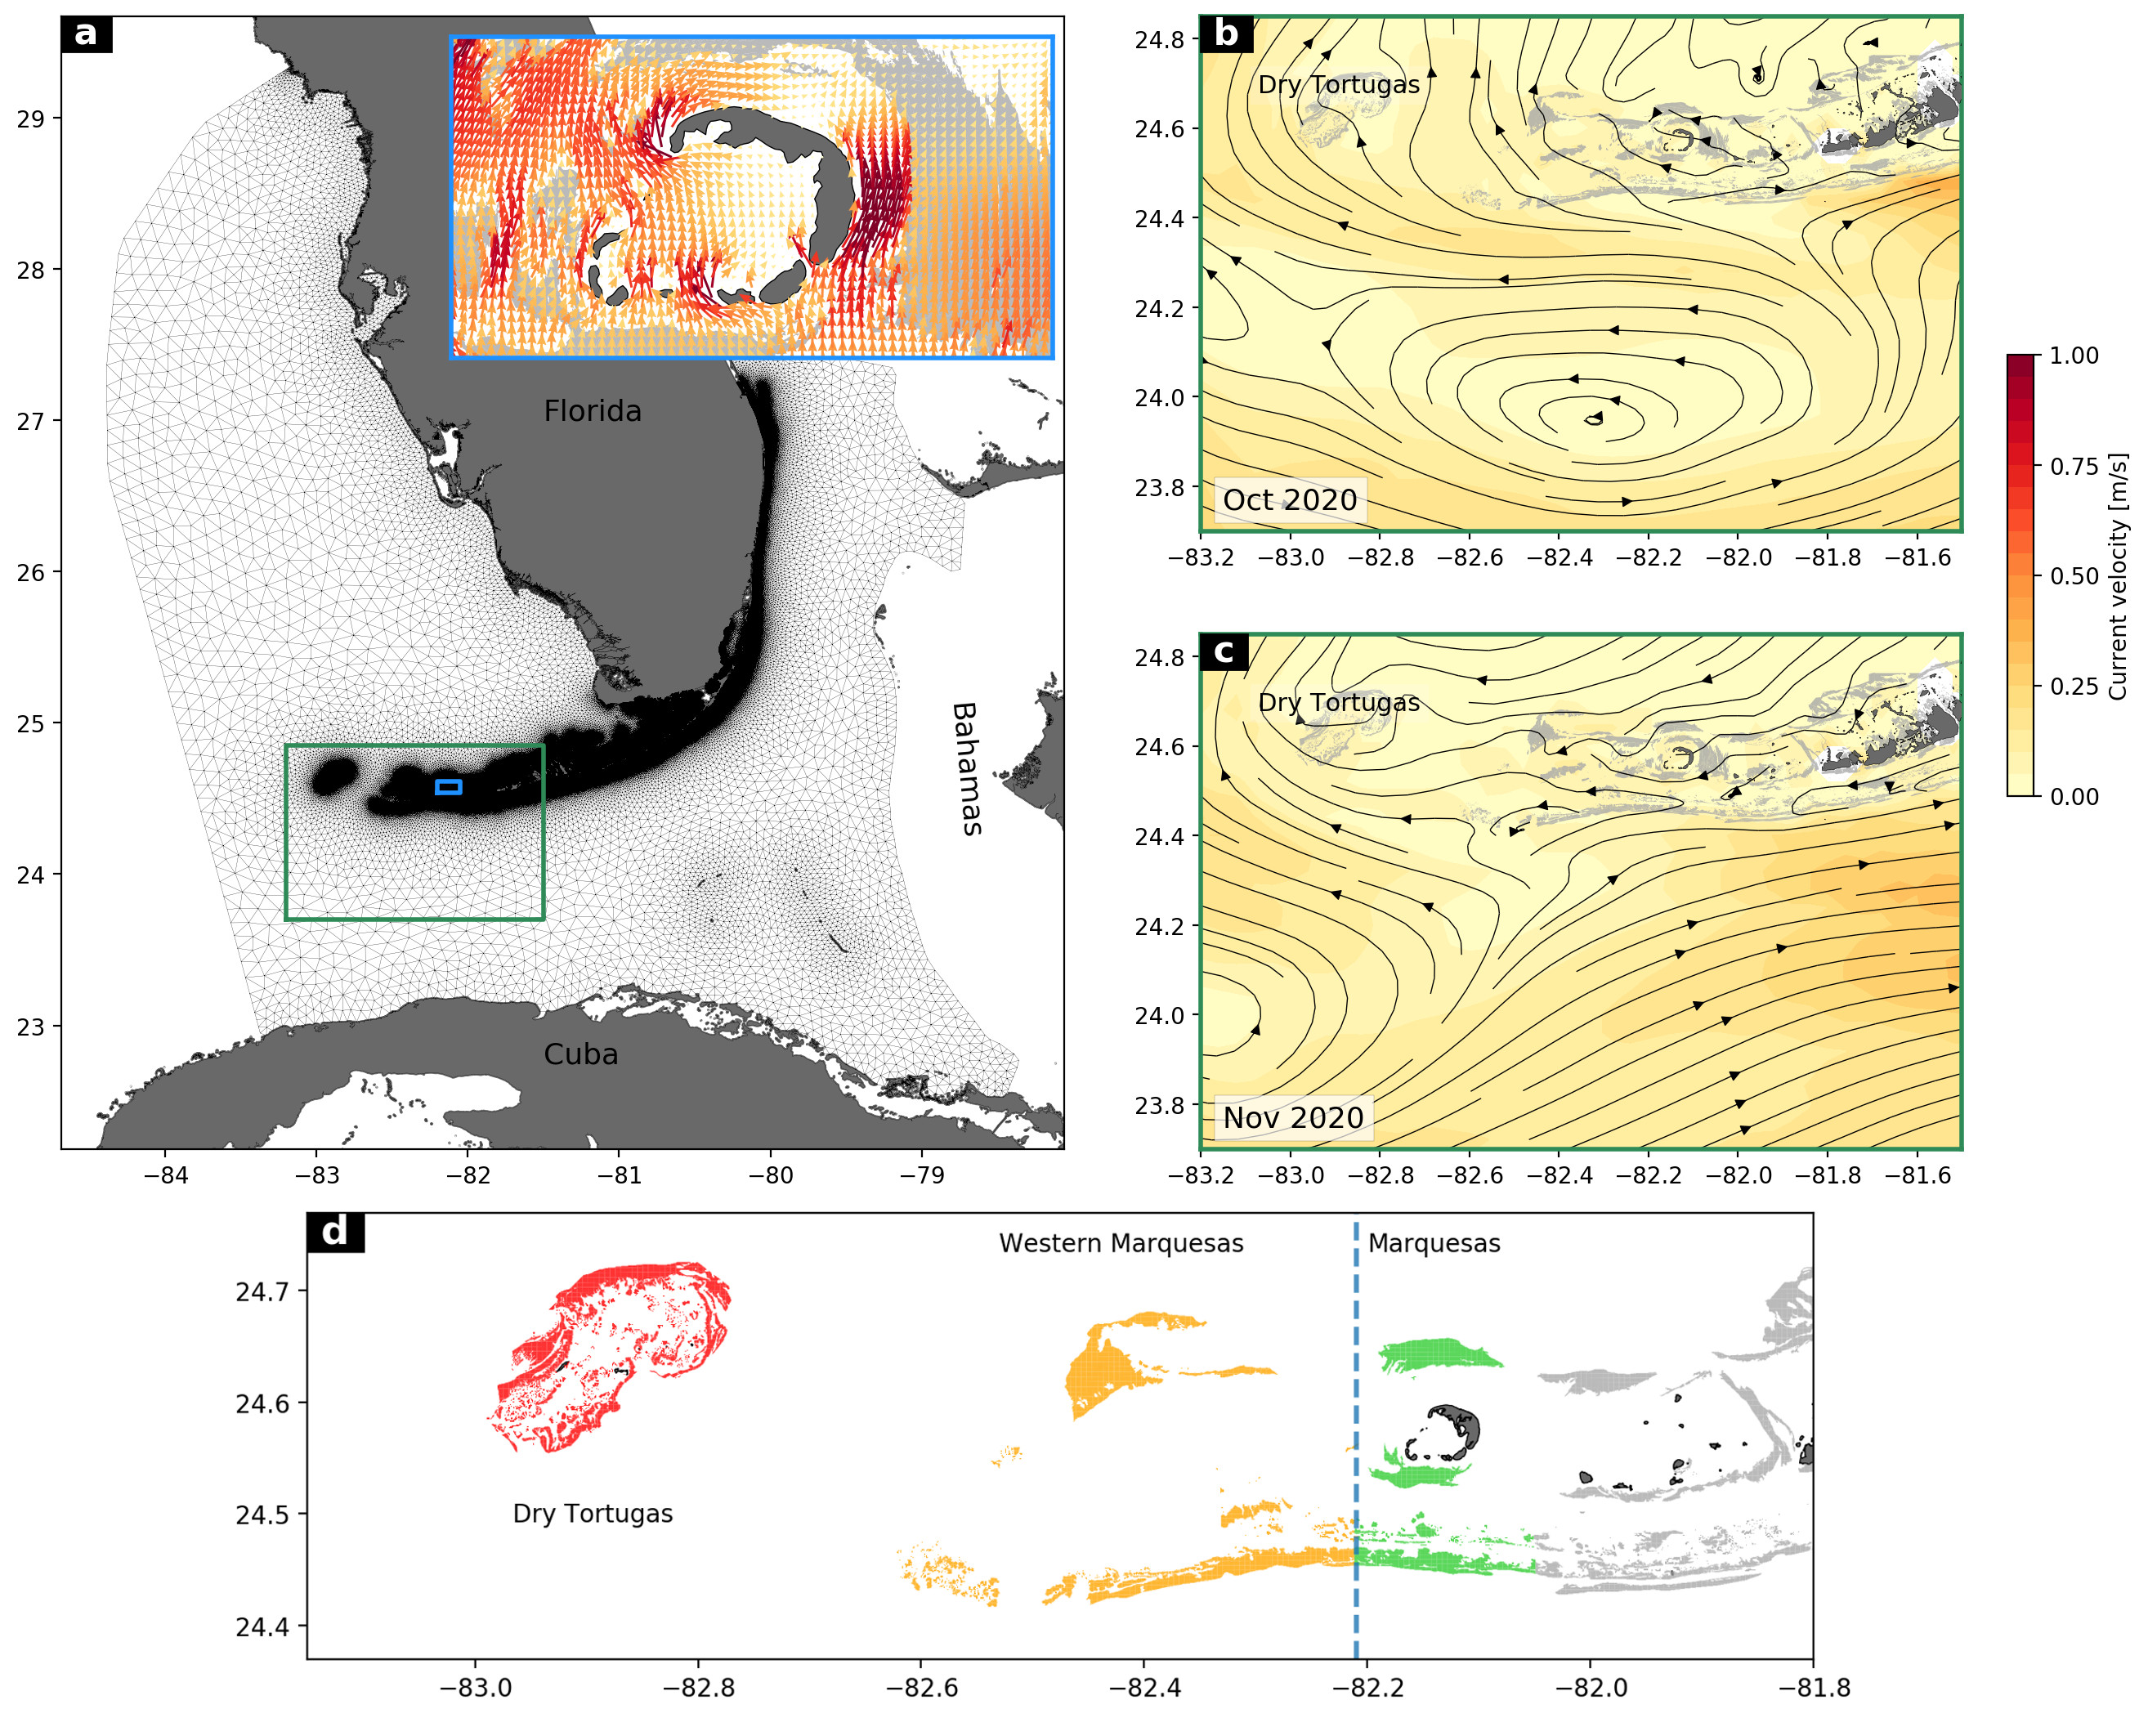
\includegraphics[width=.95\textwidth]{chapters/drto/figures/fig1.jpg}
    \caption{(a) Mesh of the computational domain and close-up view of the instantaneous currents on November 15, 2020 at 12:00 in the Marquesas (inset), (b) close-up view of the monthly-averaged circulation between the Marquesas and the DRTO in October 2020, and (c) November 2020. (d) Reefs of the areas of the DRTO, the Western Marquesas and the Marquesas, as defined in this study. Land is shown in dark gray and reefs in light gray, except in panel (d) where reefs from the Marquesas, the Western Marquesas and the DRTO are respectively shown in green, yellow and red. Streamlines indicate the presence of the Tortugas gyre in October 2020, which leads to northward currents between the Marquesas and the DRTO. In November, the gyre left its static location to transit through the Straits of Florida and currents between the Marquesas and DRTO became westward.}
    \label{fig:fig1_drto}
\end{figure}

We simulated the dispersal of disease agents throughout FCR between May 2018 and May 2021. As in \cite{dobbelaere2020coupled}, disease agents were modeled as passive particles transported by depth-averaged currents which constantly lost mass with a half-life of 30 days. We ran the particle transport model for every month between May 2018 and May 2021 and hence obtained monthly normalized connectivity matrices. An entry $C_{ij}$ of the connectivity matrix represents the probability that disease agents produced on sub-reef $i$ settle on sub-reef $j$. These sub-reefs were defined by extracting polygons from the “coral reefs and hard bottom” layer of the Unified Florida Reef Tract Map \citep{fwc2017unified} and further dividing them into 500 m $\times$ 500 m squares, generating a total of $16,823$ sub-reef polygons. Since the connectivity matrices had more than 200 million entries, they were not directly interpreted. Instead, they were represented as large networks where nodes corresponded to sub-reefs of FCR and edges corresponded to nonzero entries in the connectivity matrix. Graph-theory algorithms were then used to analyze the properties of the connectivity networks. 

To quantify the connectivity between the Marquesas and the DRTO, we defined 3 sub-regions within the sub-reefs of the western part of FCR: $(i)$ the Marquesas, $(ii)$ the Western Marquesas and $(iii)$ the DRTO (Fig. \ref{fig:fig1_drto}d). The sub-region of the Marquesas was defined as all the sub-reefs whose centroid is located between $-82.21^\circ$ and $-82.05^\circ$ longitude; the Western Marquesas included all sub-reefs between $-82.73^\circ$ and $-82.21^\circ$; and the DRTO were composed of  all the sub-reefs in our domain located west of $-82.73^\circ$ longitude. We evaluated the exchanges between two given sub-regions by identifying all edges connecting any sub-reef from one sub-region to any sub-reef from the other sub-region in our monthly connectivity networks. We then defined a connectivity indicator by multiplying the number of these direct edges by their mean connection probability. This indicator was computed monthly between May 2018 and May 2021 to evaluate the connectivity $(i)$ from the Marquesas to the DRTO, $(ii)$ from the Western Marquesas to the DRTO and $(iii)$ from the Marquesas to the Western Marquesas.

The spatial information of the network can be used to predict which part of the DRTO was likely to be first exposed to potential disease agents via hydrodynamic connections. We built a monthly spatial vulnerability indicator by summing the probabilities of all edges connecting sub-reefs of the Marquesas and the Western Marquesas to a given sub-reef of the DRTO. Sub-reefs of the DRTO with larger values of this indicator would have a larger cumulative likelihood of being infected during the simulated month. Such areas would thus be more likely to be the "entry points" of SCTLD in the DRTO during the month, as they were the destination of more pathways with larger exchange probabilities. A similar indicator can be computed for the Marquesas and the Western Marquesas by summing the probabilities of the edges connecting a given sub-reef of these sub-regions to the DRTO. Sub-reefs with higher value of this source indicator would be more likely to initiate the propagation of the disease to the DRTO, as they were the origin of more connectivity pathways with larger exchange probabilities. Model predictions were then compared to actual observations of the first cases of SCTLD in the DRTO collected on the interactive map of \cite{kramer2019map}. 

To understand the effect of the ocean circulation on disease transmission, we computed the monthly-averaged circulation for each simulated month. These residual currents were used to visually assess the presence of a Tortugas gyre during that month, i.e. the presence of eastward moving eddies persisting on temporal and spatial scales consistent with the description of \cite{lee1994evolution} in the vicinity of the DRTO. Moreover, we defined an axis from the Marquesas to the DRTO over which we averaged the monthly residual currents. These temporally and spatially averaged currents were used as a proxy of the circulation between the Marquesas and the DRTO during each simulated month.

\section{Results}
The evolution of the monthly connectivity indicator suggests that there were no exchanges from the Marquesas and the Western Marquesas to the DRTO between February and October 2020, and between January and May 2021 (Fig. \ref{fig:fig2_drto}a). This is quite remarkable as outside of these periods of low connectivity, there were no periods greater than four months without exchange from both the Marquesas and the Western Marquesas between May 2018 and May 2021. Furthermore, February-October 2020 and March 2021 were the only months characterized by mean currents with an eastward component between the Marquesas and the DRTO (Fig. \ref{fig:fig2_drto}b). These periods of low connectivity and circulation inversion appeared correlated with the presence of eddies near the DRTO, as Tortugas gyres were observed during most months with no simulated connections to the DRTO. Additionally, no exchange occurred in September 2019 or from January to February 2021, during which a strong southward mean circulation occurred between the Marquesas and the DRTO (Fig. \ref{fig:fig2_drto}b). This suggests that southward currents might also act as a barrier to disease propagation by flushing away disease agents south to the GoM. Connectivity from the Marquesas to the Western Marquesas was never completely interrupted during our simulated period (Fig 2a). Nonetheless, periods of low connectivity to the DRTO occurred in the presence of Tortugas eddies (April-June 2020) and southward circulation (February 2021). This suggests that propagation of disease agents from the Marquesas to the Western Marquesas was routinely possible, even though exchanges may have been hindered by the local circulation. This latter result is consistent with the observed westward propagation of the disease in the Marquesas between October 2019 and August 2020.

\begin{figure}
    \centering
    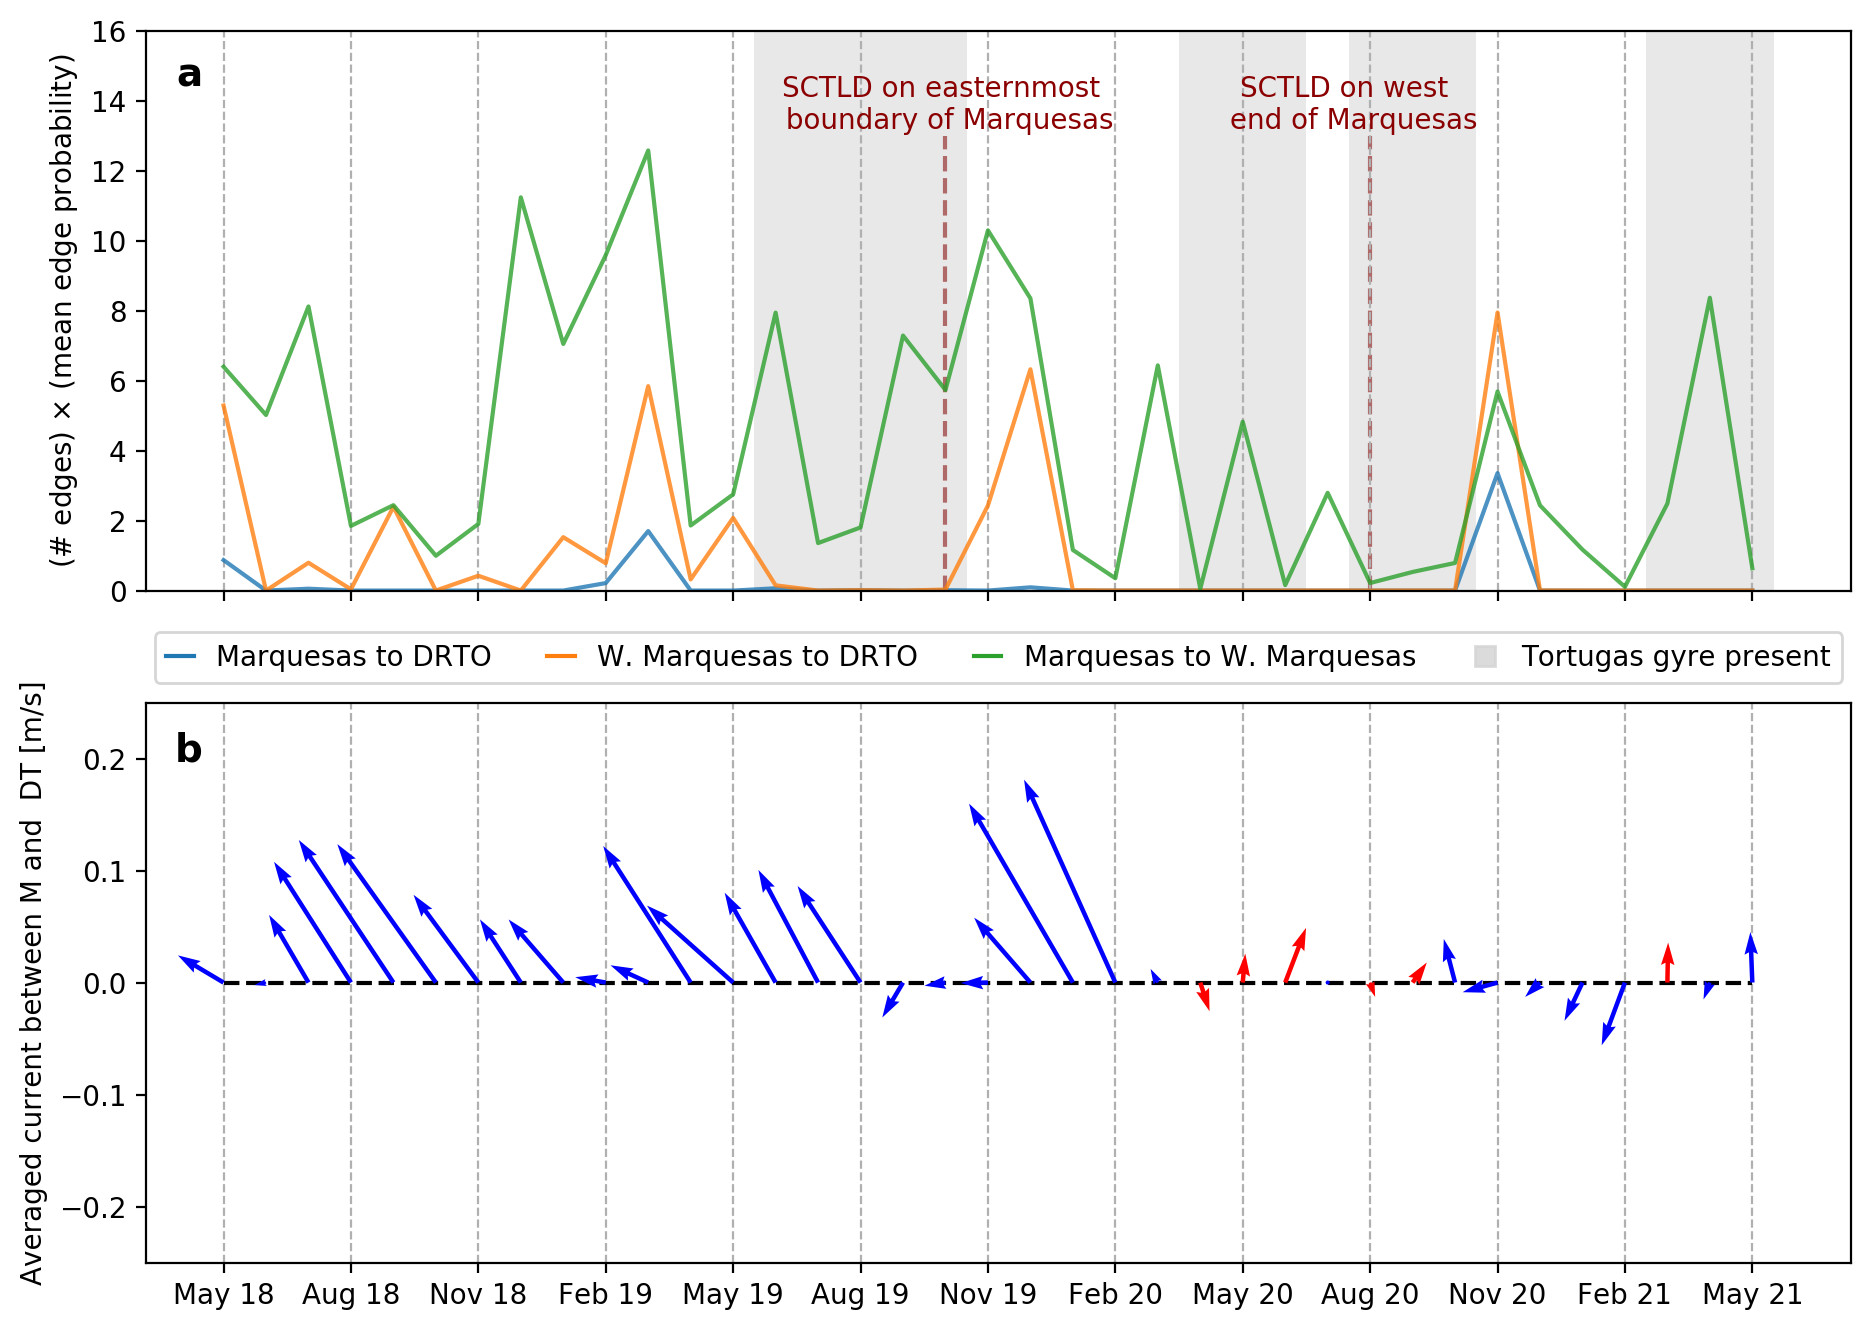
\includegraphics[width=.9\textwidth]{chapters/drto/figures/fig2.jpg}
    \caption{(a) Monthly connectivity indicator between the Marquesas and the DRTO (blue), the Western Marquesas and the DRTO (orange) and the Marquesas and the Western Marquesas (green) between May 2018 and May 2021. Months during which Tortugas gyres were observed in the ocean model outputs are highlighted in grey. Milestones of the observed propagation of the SCTLD through the Marquesas are indicated by dark red dotted lines. (b) Monthly mean currents between the Marquesas and the DRTO between May 2018 and May 2021. Mean ocean circulation with an eastward component is highlighted by red arrows.}
    \label{fig:fig2_drto}
\end{figure}

We analyzed the spatial patterns of hydrodynamic-predicted disease connectivity to the DRTO in November 2020 in more detail as the model suggested this was the month with the highest transmission probability due to high hydrodynamic connectivity. The most probable pathways to the DRTO originated mainly from southern reefs located between the Marquesas and the Western Marquesas, as well as from reefs of the northwestern end of the Western Marquesas (Fig. \ref{fig:fig3_drto}). This suggests that sub-reefs of these areas were more likely to send disease agents to the DRTO in November 2020. Conversely, no connection with large probability originated from the southwestern tip of the Western Marquesas, suggesting that they had very low potential to spread the disease to the DRTO. \\
The reefs with the highest vulnerability indicator value in November 2020 were mostly located on the eastern part of the DRTO, suggesting that these reefs were more likely to be affected during this month (Fig. \ref{fig:fig4_drto}a). More specifically our results suggest that an area of higher vulnerability was present in the vicinity of the locations where SCTLD was observed in May 2021. Vulnerability was the lowest on inner sub-reefs of the DRTO as they are not directly connected to the reefs of the Western Keys. This suggests that the disease must first spread through the outer reefs to reach them. The source indicator values confirm that disease transmission to the DRTO is more likely to originate from southern reefs at the interface between the Marquesas and the Western Marquesas, and reefs on the northwestern end of the Western Marquesas (Fig. \ref{fig:fig4_drto}b).

\begin{figure}
    \centering
    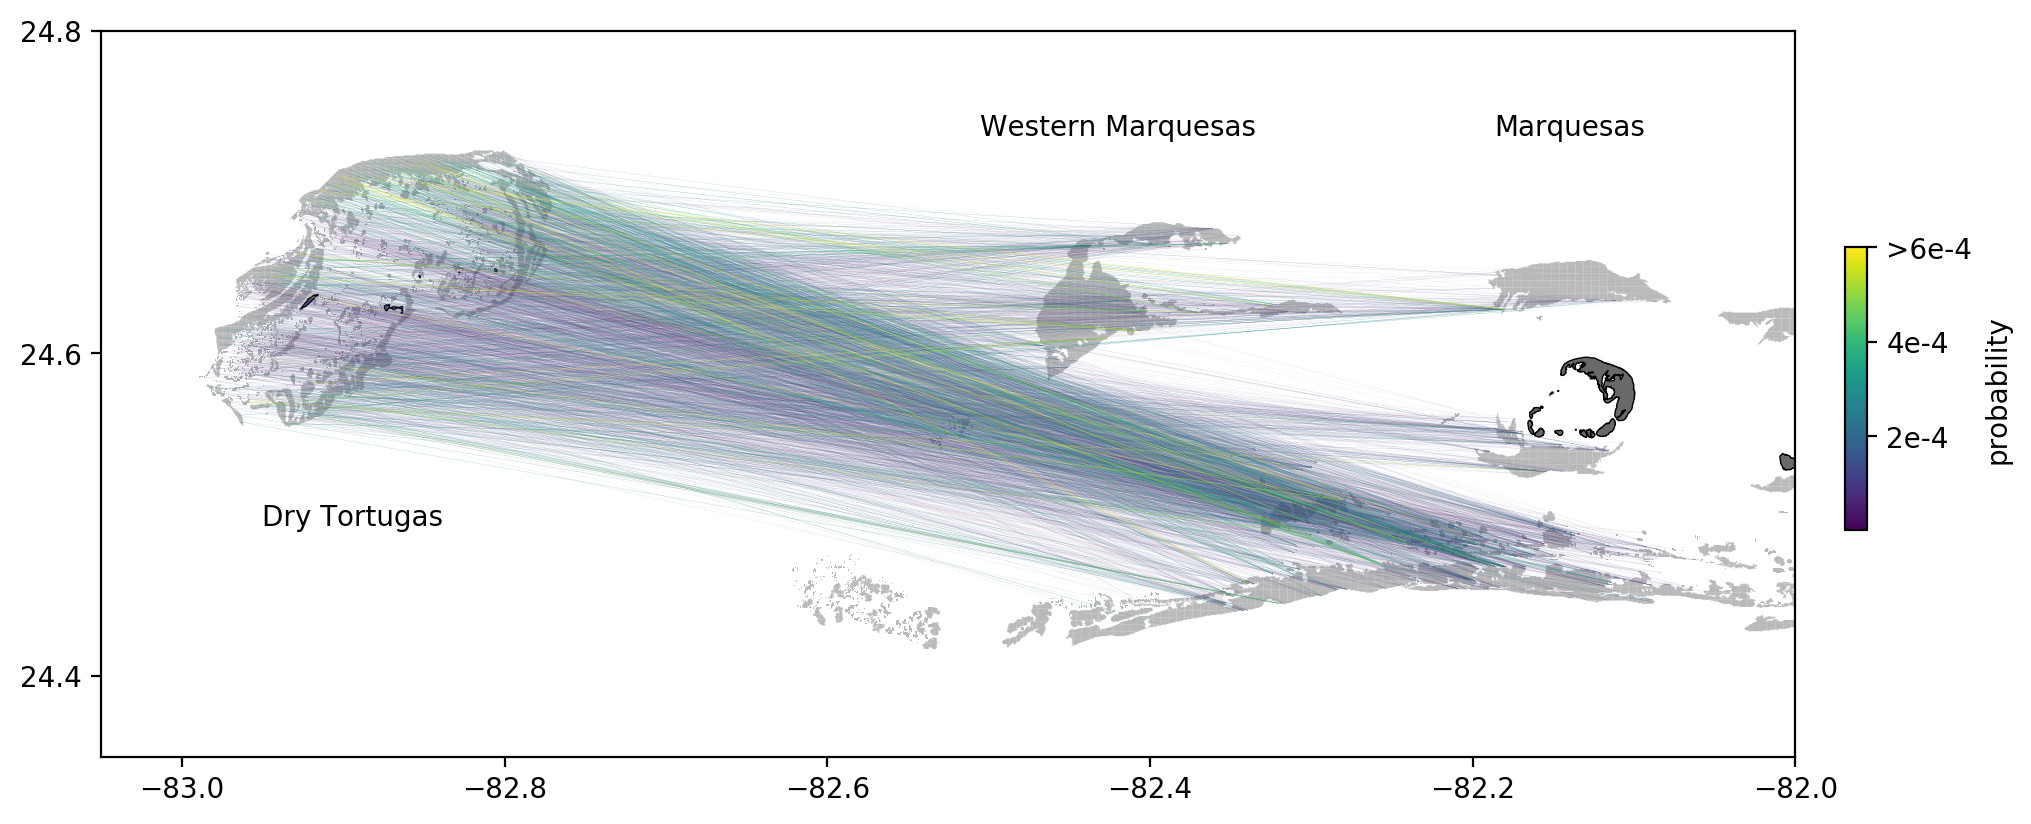
\includegraphics[width=.9\textwidth]{chapters/drto/figures/fig3.jpg}
    \caption{Edges with largest connection probability to each sub-reef of the DRTO from the Marquesas and the Western Marquesas in November 2020. Connections mostly originated from the southern reefs between the Marquesas and Western Marquesas, and from the northwestern reefs of the Western Marquesas. Reefs are highlighted in light gray while islands are shown in dark gray.}
    \label{fig:fig3_drto}
\end{figure}

\begin{figure}
    \centering
    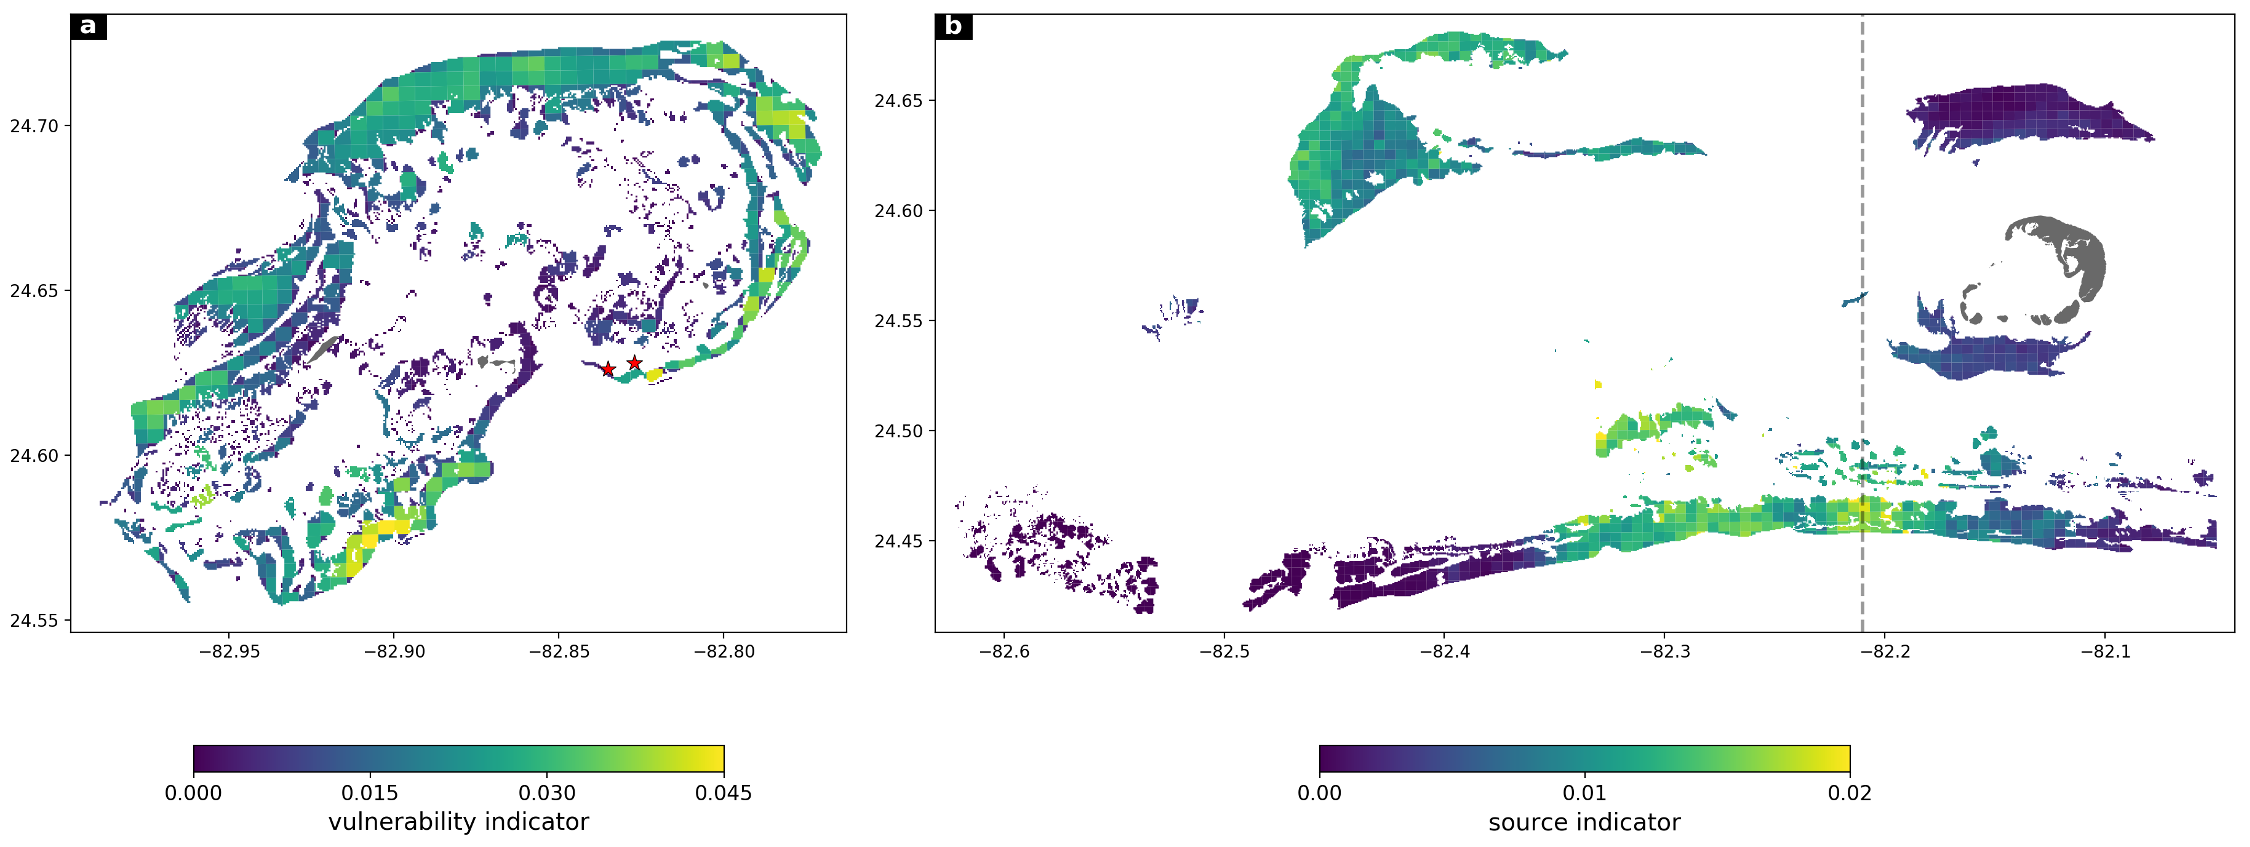
\includegraphics[width=.9\textwidth]{chapters/drto/figures/fig4.png}
    \caption{ (a) Vulnerability indicator value of all sub-reefs of the DRTO in November 2020. Eastern reefs of the DRTO appear most vulnerable to the disease. Locations where the SCTLD was observed in the DRTO are indicated by red stars (b) Source indicator value in November 2020 for every sub-reef of the Marquesas and the Western Marquesas. Northwestern reefs of the Western Marquesas and southern reefs between the Marquesas and the Western Marquesas show a higher transmission potential to the DRTO. Main islands are shown in dark grey, separation between the Marquesas and the Western Marquesas is indicated by a dashed line.}
    \label{fig:fig4_drto}
\end{figure}


\section{Discussion and conclusion}
Our results show that the eddies generated by the LC/FC system strongly influence the connectivity between the Marquesas and the DRTO. Mesoscale eddies modify the westward coastal currents by breaking them through strong cross-shore flow regime \citep{kourafalou2012florida}, as illustrated for October 2020 in Fig. \ref{fig:fig1_drto}. \cite{lee1994evolution} hypothesized that such cross-shore flow could impact the transport of larvae spawned in the Florida Keys and cause their retention on the West Florida Shelf for periods on the order of 6 months. As Tortugas eddies may remain stationary near the DRTO for up to 120 days \citep{fratantoni1998influence}, they may thus act as barriers for the exchanges between the Marquesas and the DRTO for extended periods of time. Moreover, the passage of mesoscale eddies was identified as one of the physical mechanisms likely to deliver larvae from the DRTO to the Upper Keys, therefore opposing exchanges from the Marquesas to the DRTO. Our results confirm the role of mesoscale eddies as potential barriers to connectivity between these two regions as most months during which Tortugas eddies were present correspond to a vanishing connectivity indicator. The fact that no eddies were observed at the beginning of our simulation might be related to the identification method, based solely on visual assessment of the residual currents. A comprehensive identification of all Tortugas eddies during our simulated period would require the analysis of sea surface temperature and elevation, which is beyond the scope of the present study. While our approach might miss some Tortugas gyres, it filters out submesoscale eddies with lifespan of the order of several days. Consequently, when horizontally elongated mesoscale cyclonic streamlines are present in the computed monthly-averaged currents, they can be identified as Tortugas eddies with sufficient certainty.

The connectivity from the Marquesas to the DRTO does not seem to follow any clear seasonality and exhibits high interannual variability. Although a longer simulation period might be required to rigorously assess the presence of seasonal variations, no clear seasonal patterns were observed over the 3-year simulated period for both the connectivity indicator and the mean currents (Fig. \ref{fig:fig2_drto}). In this regard, the boundary of the West Florida Shelf significantly differs from the inner shelf, which exhibits a robust cycle between summer and winter months \citep{liu2012seasonal}. Furthermore, our results indicate that the connectivity from the Marquesas to the DRTO strongly varies from year to year. This is best illustrated in March-September 2020, during which no connectivity was observed for an extended period of time and the dominant currents between the Marquesas and the DRTO had an eastward component. Such behavior was not observed during the rest of the simulation. These results are consistent with the strong variability of the LC/FC system, which strongly impacts circulation near the DRTO. \cite{lee1994evolution} and \cite{fratantoni1998influence} first described the influence of the LC penetration and ring shedding dynamics in the GoM on the formation of eddies near the DRTO. \cite{kourafalou2018physical} then further identified that LC eddy separation events were related to the formation of southward currents over the Pulley Ridge reefs and the perturbation of the slope stratification on the Southwestern Florida Shelf. The detachment of anticyclonic eddies from the main LC affects in turn the position of the FC, which strongly impacts eddy activity near the DRTO and the Marquesas, either through the formation of local eddies or the retention of remote eddies near the DRTO \citep{kourafalou2012florida}. These variations of the FC position have been shown to have no seasonal pattern with strong interannual variability and generate complex eddy to eddy interactions \citep{kourafalou2012florida}. Furthermore, the DRTO area was identified as a region of significant importance for the ecology of the West Florida Shelf, as contacts with the LC cause the inflow of nutrients that modify water properties on the shelf \citep{weisberg2003local,liu2016offshore}. \cite{weisberg2017loop} further hypothesized that these contacts might in turn impact the penetration of the LC in the GoM.

We have shown that the ocean circulation, and in particular the presence or absence of eddies shed from the Florida Current, coincides with the timing of initial SCTLD observations and likely transmission to the DRTO. However, it is important to note that it is currently not possible to determine whether SCTLD is caused by a novel pathogenic agent or simply a variant of a previously existing disease that causes tissue loss on corals. The DRTO has experienced episodic outbreaks of tissue loss in years prior to 2020 (see \citealp{frrp2018}). These previously documented tissue loss events occurred during the summer months within isolated reef sites and primarily affected one genus of corals, \textit{Orbicella}. Although the ecology of SCTLD documented from 2014 to the present differs from these previous reports, until pathogenic agents are identified, the positive identification of a particular coral disease, such as SCTLD, will remain presumptive. However, past studies indeed suggest SCTLD is likely caused by a waterborne agent regardless of the particular pathogen at play. As such, intense eddy activity between February 2020 and May 2021 would have largely prevented the exchange of disease agents westward, with the exceptions of November and December 2020. During those two months, the residual circulation on the southwestern Florida shelf turned westward, and thus would have allowed disease agents to reach the DRTO. The transmission of disease agents to the DRTO was most likely to occur in November 2020, when the connectivity indicator was the largest. The developed vulnerability indicator indicates that sub-reefs on the eastern part of the DRTO were more likely to be affected by the disease. These results are consistent with observation as the locations where SCTLD was observed in the DRTO are located near sub-reefs identified as highly vulnerable by our model \citep{kramer2019map}. Nonetheless, the area predicted to be vulnerable exceeds the extent of the region where signs of the disease were first observed. These discrepancies might be explained by the fact that our vulnerability indicator accounts for all potential connections to a given sub-reef. In practice, these connections only yield the transmission of disease agents if the sub-reef they originate from is affected by SCTLD. Our model might therefore overestimate the vulnerability of some sub-reefs. Moreover, due to the lack of data on coral distribution in FCR, an uniform coral density was assumed over all reefs. The impact of some reefs with low coral cover might thus be overestimated by the model. Nonetheless, we argue that our model remains a valuable tool to assess the (absence of) connectivity between the Marquesas and the DRTO.
 
Model results suggest a time lag of 5 to 6 months between the moment the hydrodynamics predicted that disease agents reached the DRTO and the moment SCTLD symptoms were observed in the DRTO. This seems to contradict the results of previous modeling and experimental studies that found SCTLD transmission times of 10 days or less \citep{dobbelaere2020coupled, meiling2021variable}. However, several elements might explain a slower development of the disease on the DRTO. First, in situ conditions might significantly differ from the ones of a controlled tank environment, potentially leading to differences in the time required for the first disease lesions to appear. Furthermore, disease transmission in the Florida Keys might occur faster as reefs can receive disease agents from several affected neighboring reefs. In the case of disease agents reaching the fully susceptible population of the DRTO, such interactions with neighboring affected colonies do not take place and the outbreak might therefore require more time to develop. Furthermore, our results suggest that corals of the DRTO could only be exposed to agents coming from the Marquesas in November and December 2020, while exposure to incoming disease agents was continuous in the Keys due to the density of the reef system. Additionally, the epidemiological parameters of \cite{dobbelaere2020coupled} were calibrated on species-averaged prevalence data in the Florida Keys, which might not be representative of the colony composition and environmental conditions in the DRTO. Finally, observational data is dependent on the frequency and spatial distribution of field missions and might therefore give an incomplete picture of the situation on the field. For example, fine scale observations of SCTLD in the Lower Florida Keys found low disease incidence (< 10 colonies) starting in October, and then disease incidence peaked in April 2019 \citep{williams2021fine}. Alternatively, one might argue that this lag between the modeled transmission of the disease agents to the DRTO and the first observations of the SCTLD indicates that the propagation of the disease was not caused by local currents. In that case, another vector, such as ballast waters, might have to be considered. However, such investigations are beyond the scope of the present study.

It is important to note that the time and location of the first observations of an outbreak do not necessarily correspond to its initiation. An epidemic might grow unnoticed during its first stages, as it first develops at a linear rate before growing exponentially. Tools such as the ones developed in the present study might therefore have helped to mitigate the SCTLD during the first stages of its development in the DRTO, before May 2021. Furthermore, this study has shown that strong eddy activity near the DRTO was likely to interrupt connectivity from the Western Florida Keys to the DRTO. Therefore, monitoring eddy activity through satellite observations of sea surface temperature and sea surface elevation anomaly \citep{kourafalou2018physical} might serve as a proxy for reef managers to estimate connectivity between these two areas. The implications of our connectivity results are not limited to the propagation of disease agents and apply to the spread of any type of propagules from the Marquesas and the DRTO. This study therefore brings additional insight on the physical and environmental connectivity in the southwestern part of FCR.

\begin{subappendices}
	\section{Validation of the model}
	
	SLIM outputs were validated against field measurements from tide gauges and ADCP in the Florida Keys and on the shelf (Fig. \ref{fig:a1}). Here, we show the comparison between observed and simulated sea surface elevation and current speed for the month of November 2020. The model accurately reproduces the observed sea surface elevation at all tide gauges (Fig. \ref{fig:a2}) with an RMSE of less than 8 cm. The current velocity on the shelf is also  well reproduced by the model, despite a slight underestimation of the southward component of the observed currents at mooring C10 and C22, located on the 25 m and 70 m isobaths respectively (Fig. \ref{fig:a3}). Using the vector correlation analysis of \citep{kundu1976ekman}, we obtained a correlation factor of 0.9 and a veering angle of 10$^\circ$ between the modeled currents and the observations at station C10. A correlation factor of 0.75 and a veering angle of 8° were obtained at mooring C22. Such values are similar to the performances of previous modeling studies on the West Florida Shelf \cite{liu2020impacts}.
		
	\begin{figure}
		\centering
		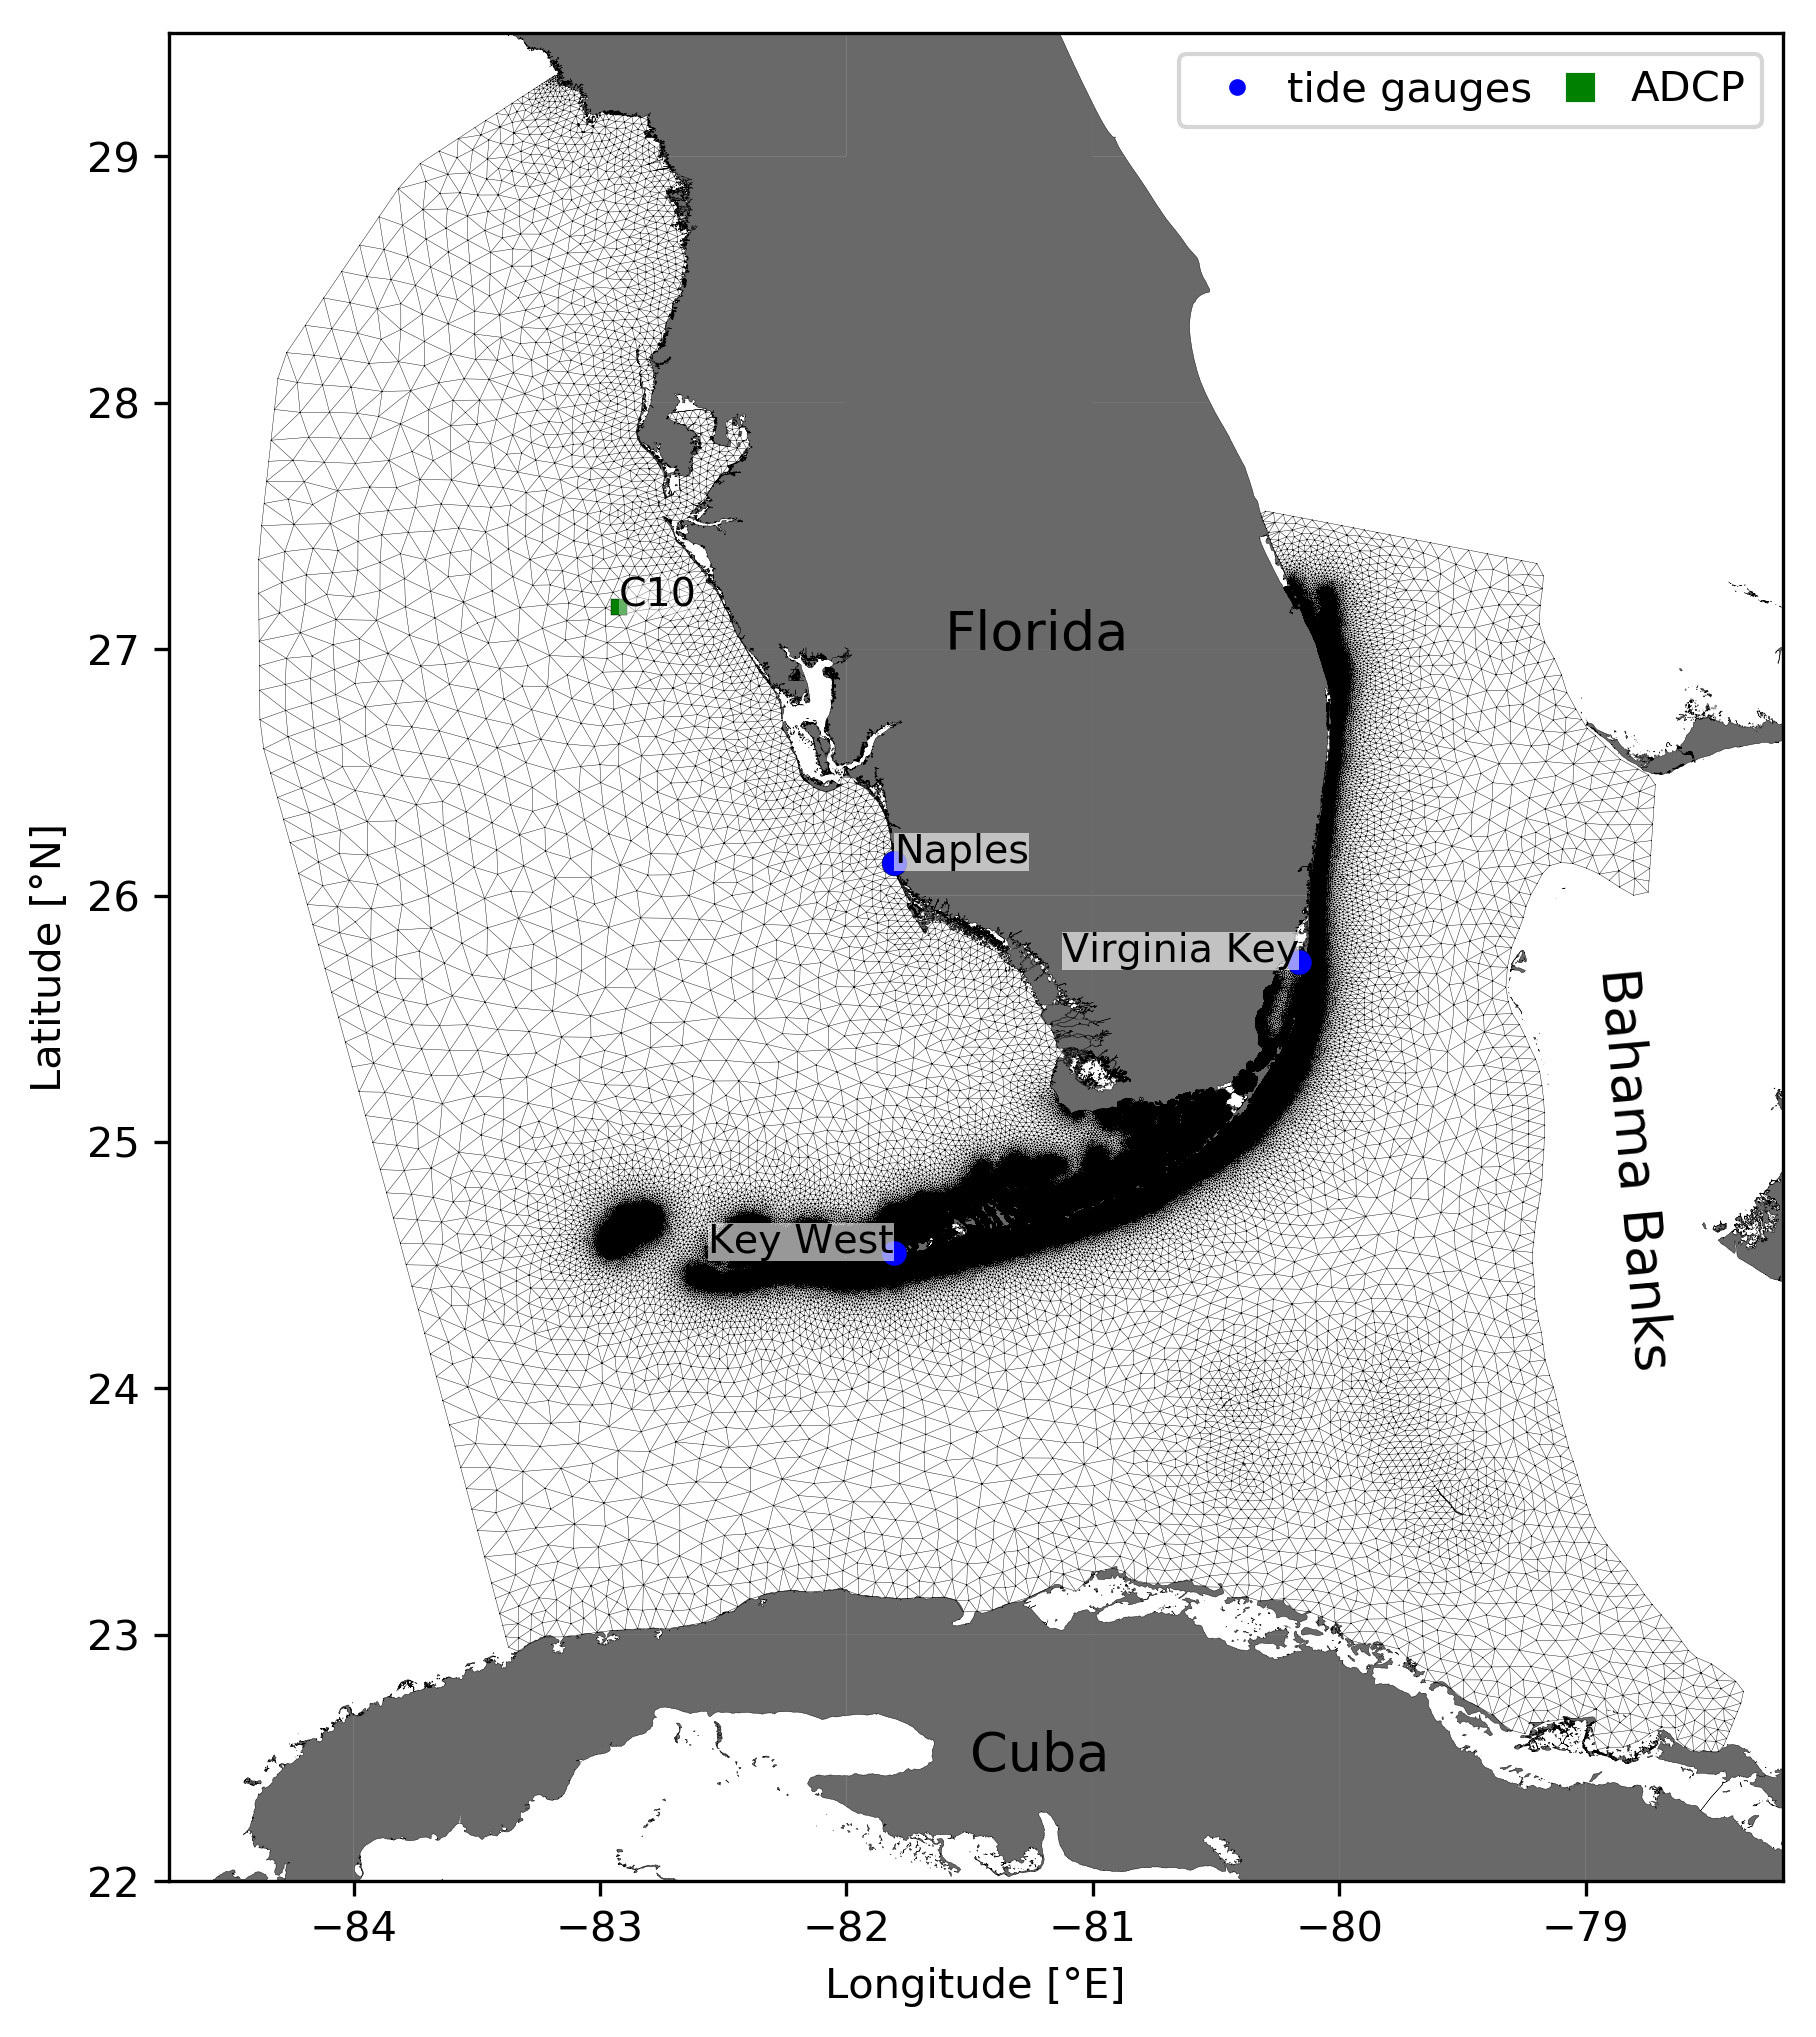
\includegraphics[width=.8\textwidth]{chapters/drto/figures/a1.JPEG}
		\caption{Mesh of the computational domain with the location of the stations used for the validation of the model outputs. Land is shown in dark gray.}
		\label{fig:a1}
	\end{figure}
	
	\begin{figure}
		\centering
		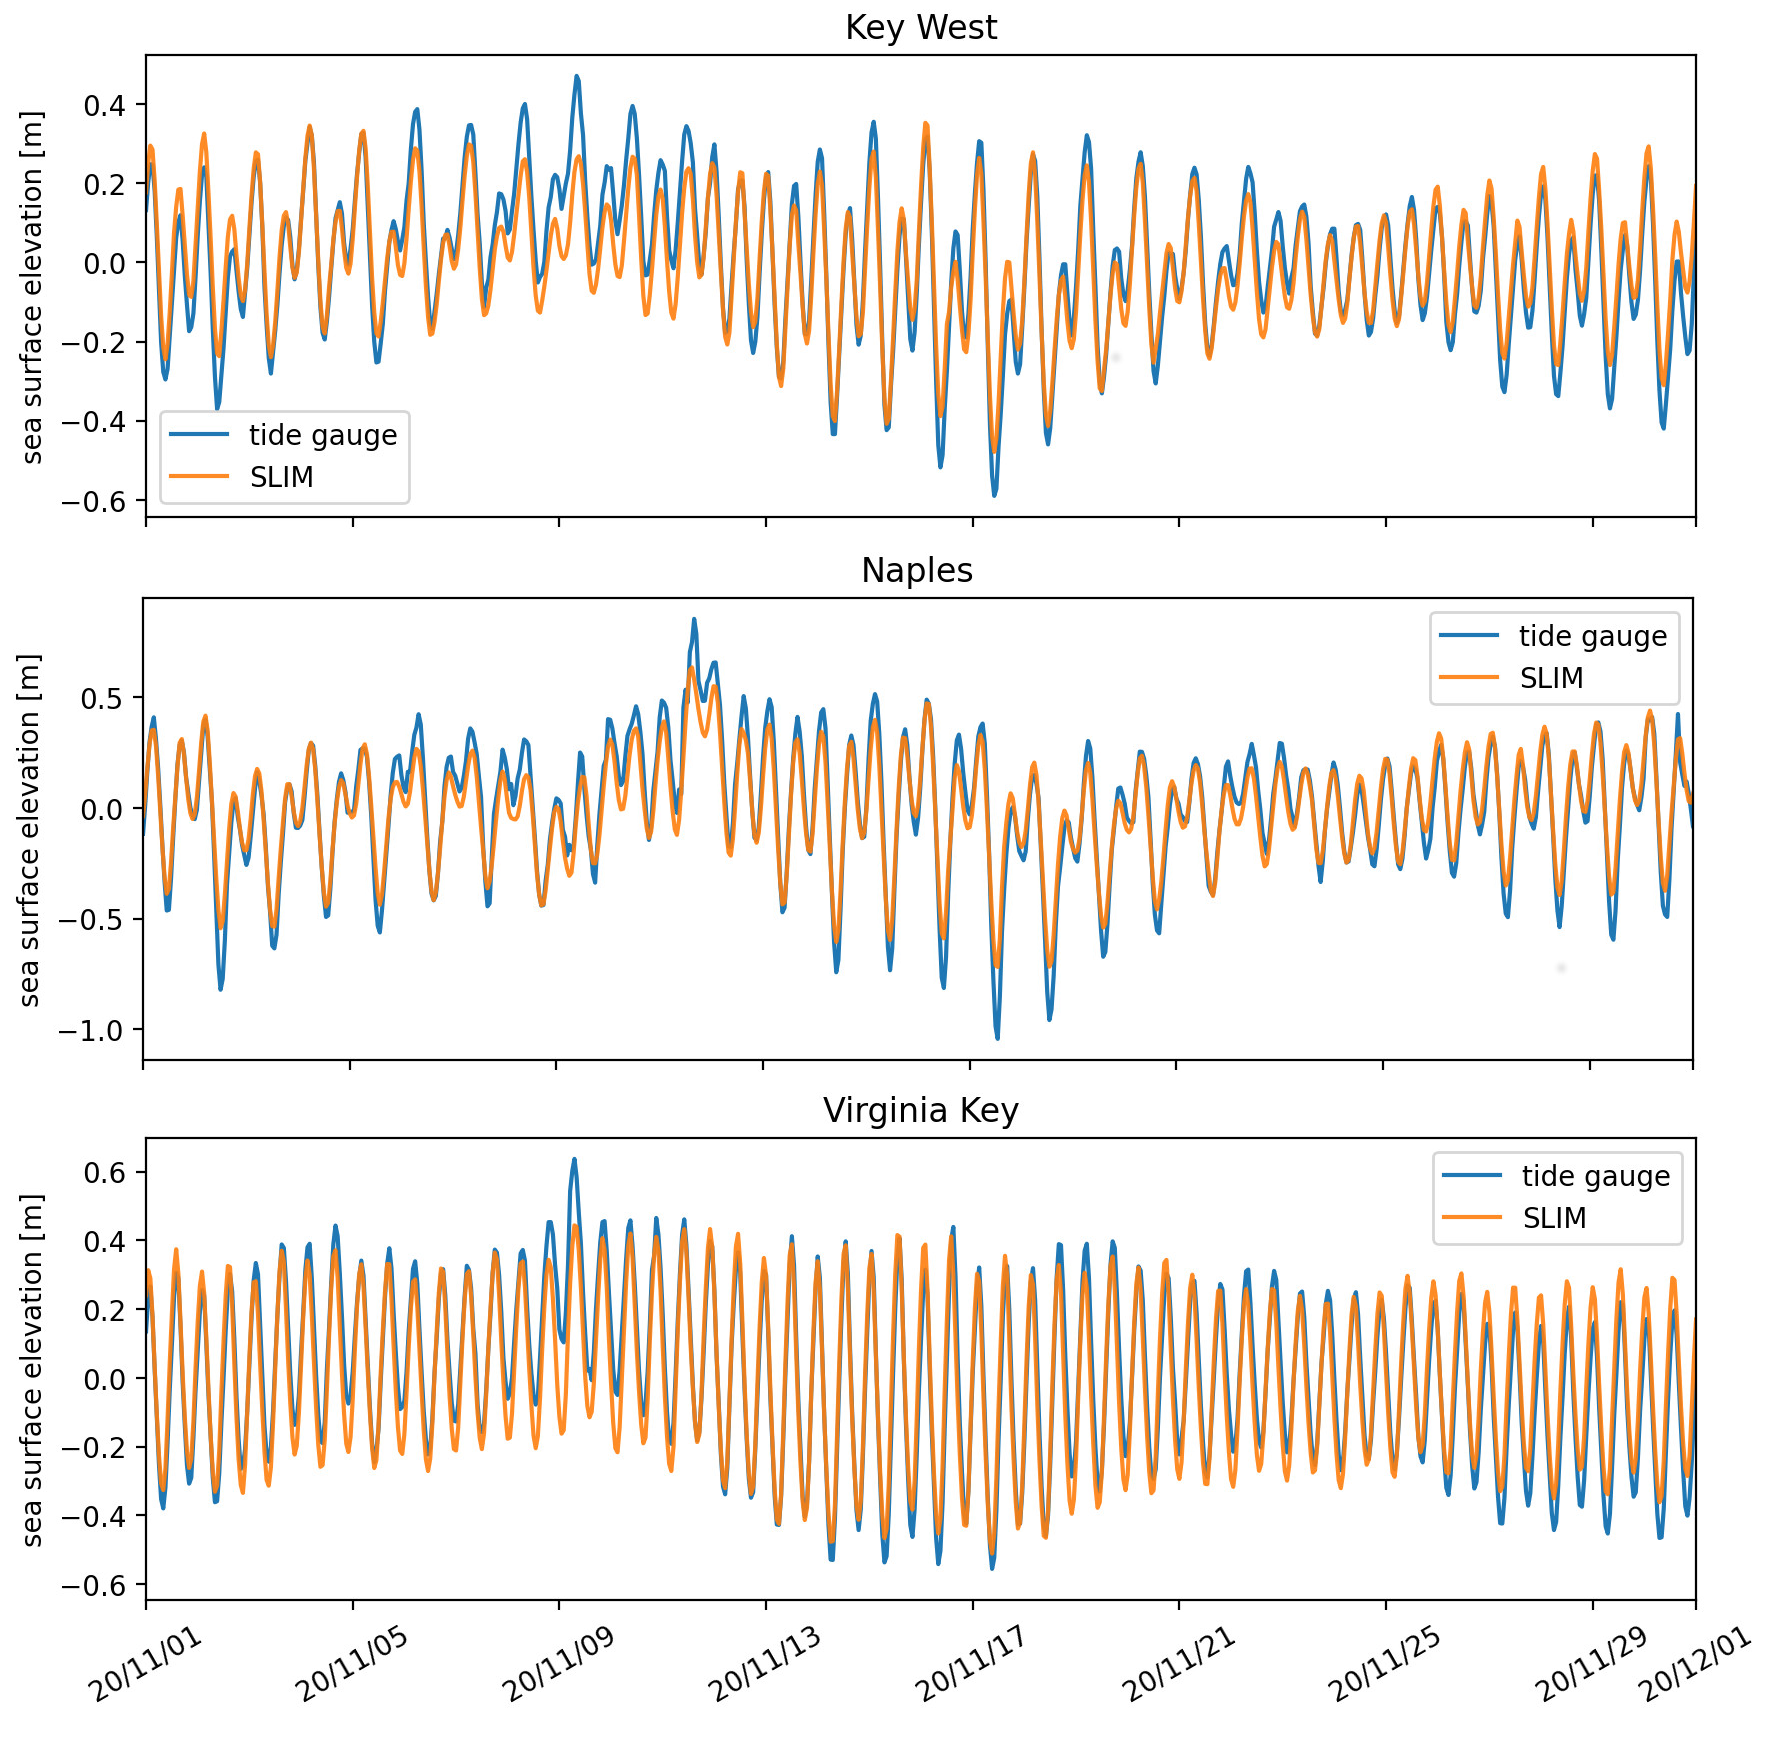
\includegraphics[width=\textwidth]{chapters/drto/figures/a2.png}
		\caption{Comparison of SLIM sea surface elevation against tide gauge elevation in November 2020. The tidal signal is well reproduced at all stations with an RMSE of less than 8 cm.}
		\label{fig:a2}
	\end{figure}

	\begin{figure}
		\centering
		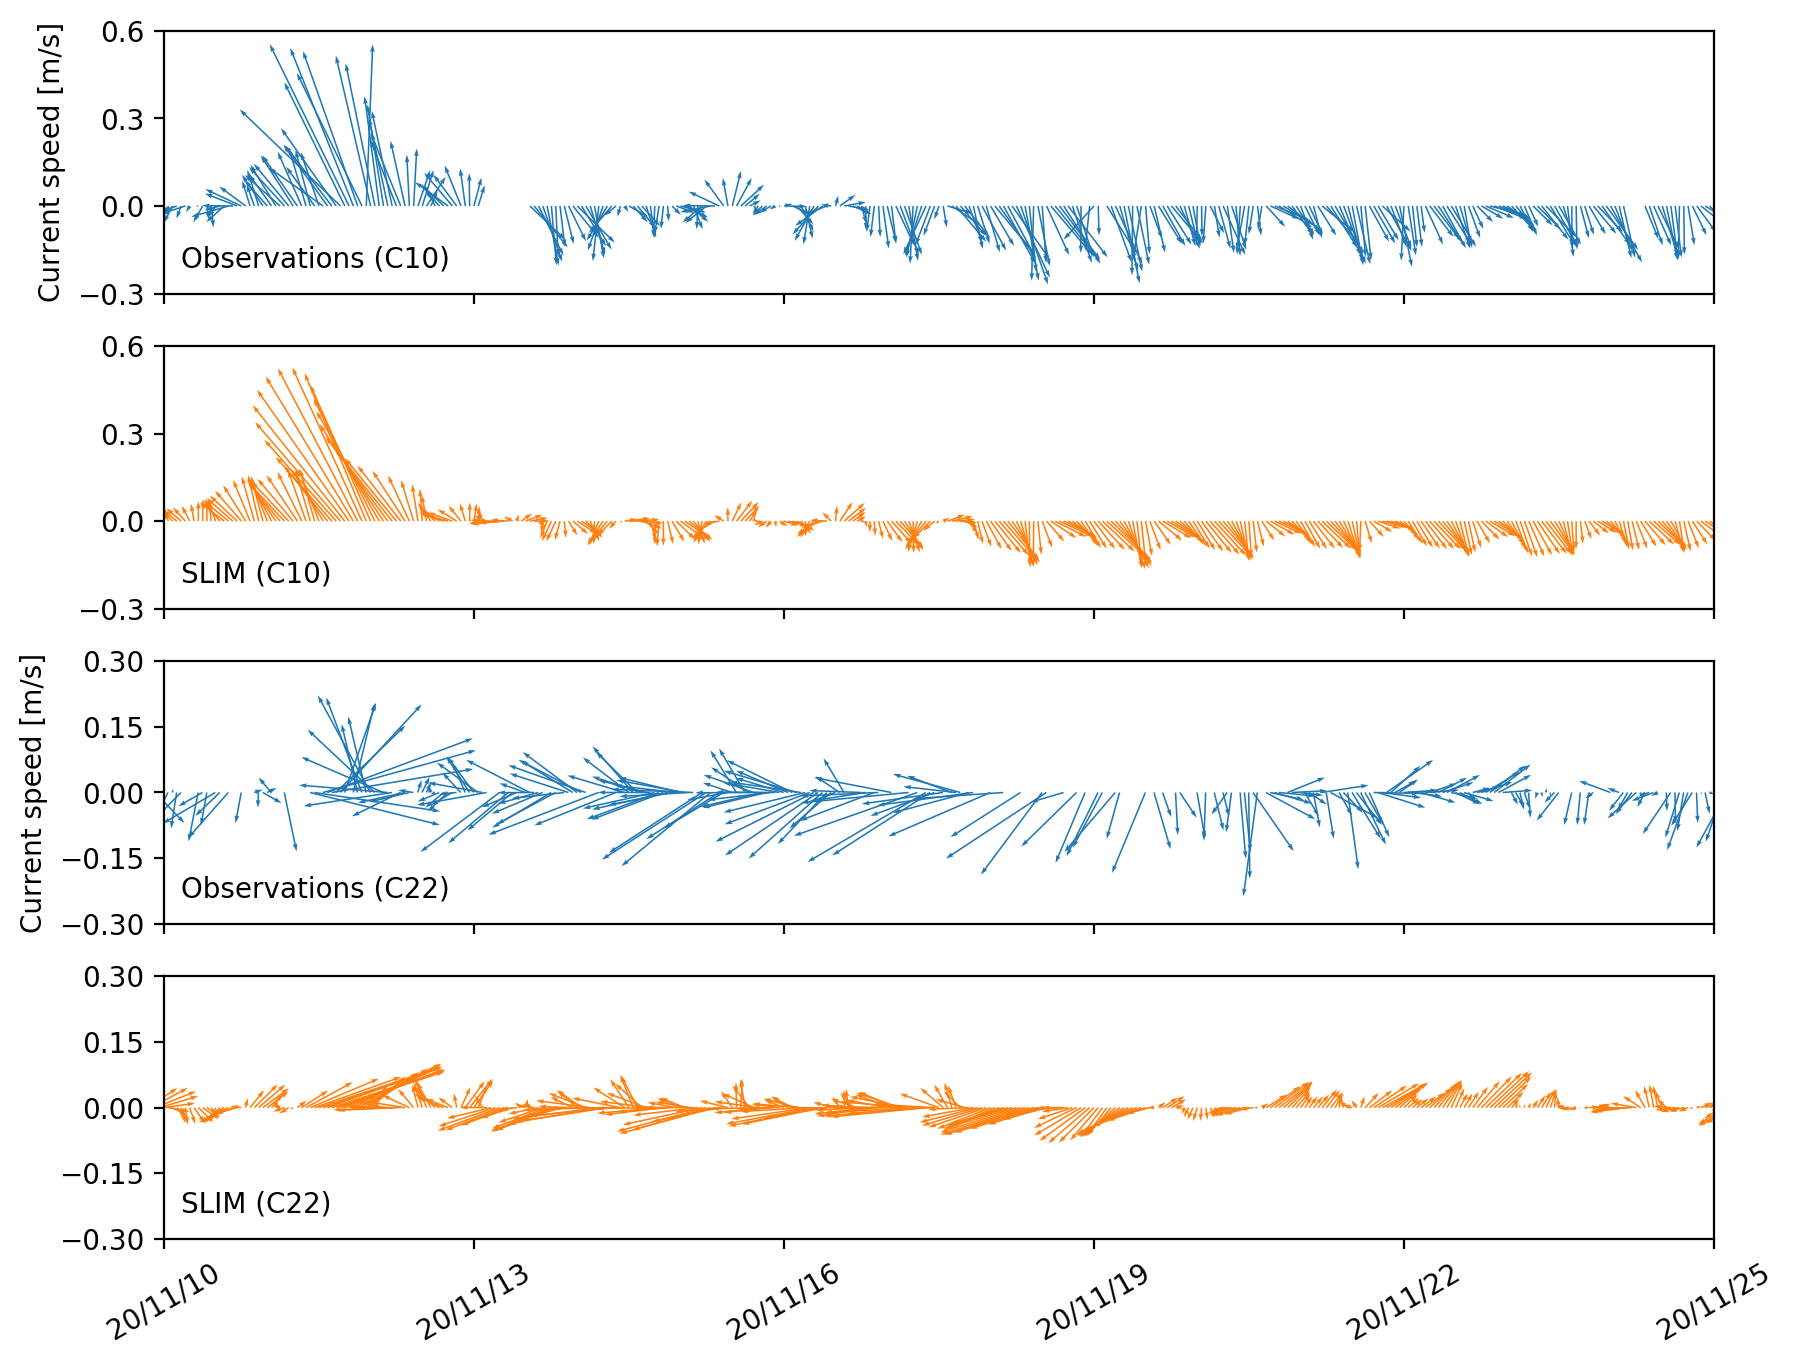
\includegraphics[width=\textwidth]{chapters/drto/figures/a3.png}
		\caption{Comparison of SLIM currents with depth-averaged ADCP measurements at mooring C10 and C22 in November 2020. Despite a slight underestimation of their southward component, currents and their oscillations are well reproduced by the model.}
		\label{fig:a3}
	\end{figure}
		
	SLIM relies on its coupling with HYCOM GoM to accurately reproduce the Loop Current (LC)-Florida Current (FC) system. HYCOM’s surface fields were therefore compared with sea surface temperature data from the Group for High Resolution Sea Surface Temperature (GHRSST; \url{https://www.ghrsst.org/}). HYCOM reproduces well the penetration of the LC in the Gulf of Mexico (Fig. \ref{fig:a4}), which is key to simulating the eddy activity linked to the meandering of the FC near the DRTO.
	
		\begin{figure}
		\centering
		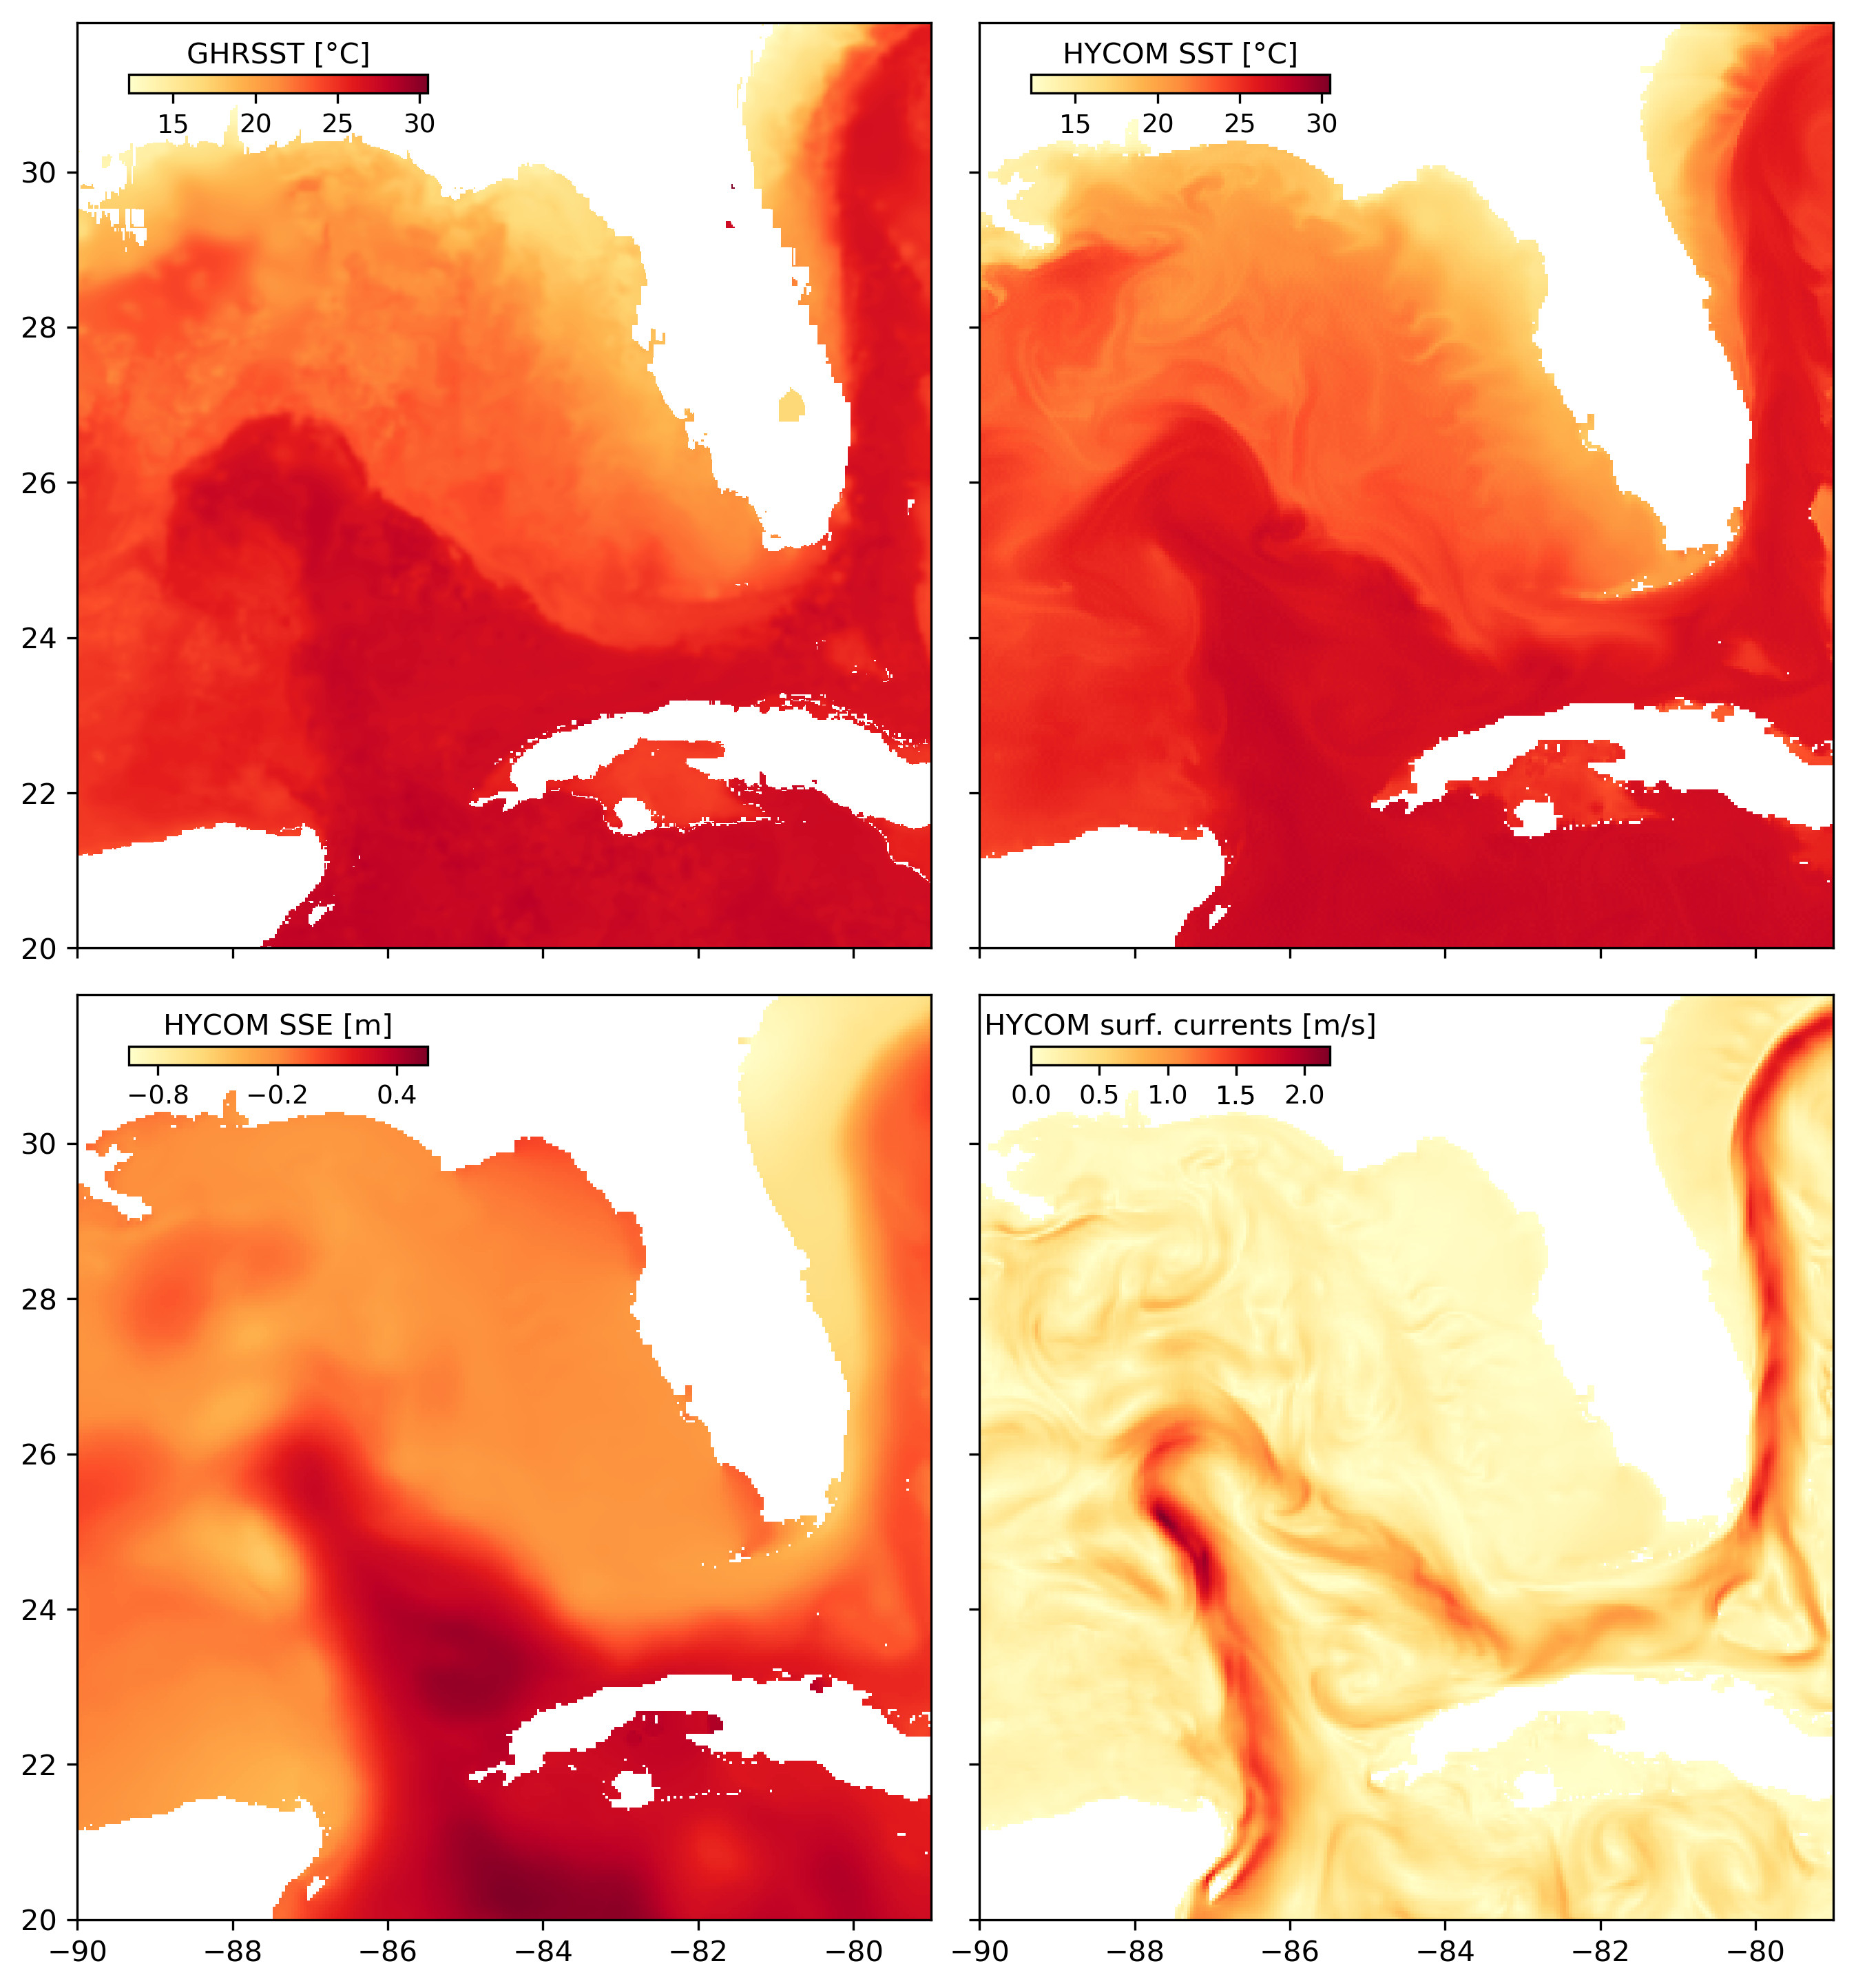
\includegraphics[width=\textwidth]{chapters/drto/figures/a4.JPEG}
		\caption{Comparison of (\textbf{A}) satellite-derived sea surface temperature from the Group for High Resolution Sea Surface Temperature (GHRSST) against (\textbf{B}) sea surface temperature, (\textbf{C}) sea surface height (SSH) and (\textbf{D}) surface current magnitude modeled by HYCOM. All panels are snapshots of November 15, 2019 at 0000 UTC.  The model reproduces well the penetration of the LC in the Gulf of Mexico.}
		\label{fig:a4}
	\end{figure}
	
\end{subappendices}
\mychapter{The onset of the SCTLD outbreak and the PortMiami Deep Dredge Project} \label{chap:onset}
\chaptermark{Onset of SCTLD and PortMiami Deep Dredge Project}  

This chapter is based on the following article:
\begin{list}{}{%
\setlength{\topsep}{0pt}%
\setlength{\leftmargin}{0.23in}%
\setlength{\listparindent}{-0.23in}%
\setlength{\itemindent}{-0.23in}%
\setlength{\parsep}{\parskip}%
}%

\item \textbf{Dobbelaere, T.}, other co-authors TBD, \& Hanert, E. Early transmission dynamics of a deadly coral disease and its connection with the PortMiami Deep Dredge Project. (planned submission to \textit{Marine Pollution Bulletin})
\end{list}

\begin{abstract}
    For the last 8 years, Florida's Coral Reef (FCR) has suffered from severe coral loss caused by stony coral tissue loss disease (SCTLD). The outbreak reportedly initiated near Virginia Key in September 2014, during the deepening of the Port of Miami (PoM) shipping channel, that took place between November 20, 2013 and March 16, 2015. The disease then spread to the entirety of FCR, likely through waterborne transmission. Although the causative agent of SCTLD remains unknown, there is evidence that sediments can act as vector for the disease. Here we evaluate whether sediments produced or resuspended during dredging operations could have reached reefs where the disease was first reported and assess whether the timing of these sediment fluxes was consistent with the observed spread of the disease. We evaluated the transport of sediments caused by the expansion of PoM between November 2013 and September 2014 using a quasi-3D sediment transport model forced by currents from the high-resolution coastal ocean model SLIM. A particular attention was paid to the non conventional dredging operations performed without pumping the produced chopped rock particles. Our results suggest that the dredging had close to no direct impact on the coral reefs of Virginia Key through sediment flux and sedimentation. However, a significant fraction of the sediments produced reached monitoring sites where the disease was reported prior to September 2014, suggesting that the dredging might have played a role in the onset of the outbreak at these sites. Furthermore, using a biophysical disease agent transport model, we show that waterborne transmission from one of these sites to Virginia Key was possible before September 2014. This study brings new insight on the role that the deepening of PoM might have played in the onset of one of the worst coral outbreaks on record in the Caribbean.
\end{abstract}

%\newpage



\section{Introduction}

%  PARAGRAPH DISEASES IN GENERAL
Coral diseases are a major threat to coral reef ecosystems and have led to significant declines in coral cover especially within the Caribbean region \citep{richardson1998coral, sutherland2004disease, aronson2001white, harvell2007coral, brandt2009dynamics}. One of the latest and the most damaging outbreak to date in Florida's Coral Reef (FCR) is the stony coral tissue loss disease (SCTLD) \citep{noaa2018}. First observed off the coast of Miami in 2014 by \cite{precht2016unprecedented}, the disease has since spread through the entire FCR \citep{muller2020spatial,dobbelaere2022} and has been observed in several territories of the Caribbean \citep{kramer2019map, meiling2021variable, estrada2021effects,heres2021ecological}. Although the causative agent of the disease remains unknown, hydrodynamics are likely to play an important role in its propagation as both modeling studies and ex situ experiments show evidence of waterborne disease transmission \citep{aeby2019pathogenesis,dobbelaere2020coupled,eaton2021measuring, meiling2021variable}. Furthermore, recent studies showed evidence that sediments can act as  a vector for the SCTLD \citep{rosales2020rhodobacterales, studivan2022reef}.

% POM
Some of the first signs of SCTLD were reported in September 26th, 2014, near Virginia Key by \cite{precht2016unprecedented}. They derived a relationship between the time of the first outbreak at monitored reefs and their geographic distance to Virginia Key. It was therefore hypothesized that the epidemic started near Virginia Key and then spread to the neighboring reef, both north and south. However, earlier signs of diseases were already reported north of Virginia Key in June 2014, at the monitoring site of N. Sunny Isles \citep{precht2016unprecedented}. All these observations occurred during the deepening of the Port of Miami (PoM) shipping channel, that took place between November 20, 2013 and March 16, 2015. The dredging was monitored twice-weekly at 26 permanent monitoring stations established within the Miami-Dade County, making it one of the most complete datasets related to a dredging project \citep{gintert2019regional}. Interestingly, disease signs were also reported at one of these monitoring stations in May 2014.

While operating in a conventional way, dredged materials were pumped from the dredge to a spider barge and then transported to the US Environmental Protection Agency designated Ocean Dredge Material Disposal Site (ODMDS) located 4.7 nautical miles offshore. However, the suction mechanism was turned off during non-conventional rock-chopping activities in order to pre-treat very hard rock contained in the Anastasia and Fort Thompson formations between December 2013 and May 2014 \citep{miller2016detecting}. The Army Corps commissioned a report that provides a back-of-the-envelope estimating this practice could have resulted in up to 33 cm deposition over 874,121 m$^2$ of reef surrounding the outer entrance channel \citep{dobbelaere2020report}. Additionally, several studies reported that the impact of the dredging was widespread \citep{miller2016detecting}, causing the death of  $> 560,000$ corals within 0.5 km of the channel \citep{cunning2019extensive} and producing sediment plumes covering up to 11 km$^2$ of coral area within 5-10 km of the dredging \citep{barnes2015sediment}.

% SEDIMENTS
Sediments released by dredging can affect the biological functions of corals in numerous ways  through turbidity and sedimentation \citep{erftemeijer2012environmental, jones2015effects}. Increased turbidity caused by the suspended sediments reduces the light available to symbiotic zooxanthellae, leading to reduced coral cover and growth. Sedimentation, on the other hand, can cause smothering or burial of coral polyps \citep{erftemeijer2012environmental}. Furthermore, both sedimentation and turbidity can significantly reduce larval recruitment by inhibiting settlement and reducing larval survival in the water column \citep{jones2015effects}. These effects are stronger with fine-grained sediments, as they cause a stronger light reduction \citep{fourney2017additive}. Additionally, fine-grained sediments such as silts have high nutrient contents, which can lead to an increased microbial activity, eventually causing anoxic conditions in the immediate vicinity of corals \citep{weber2012mechanisms}. As they release finer sediments over significantly longer periods than natural events such as hurricanes, dredging activities can thus be more harmful to corals and reef habitat compared to other types of sedimentation \citep{cunning2019extensive}.

% ON ENTRE DANS LE VIF DU SUJET
Nonetheless, \cite{gintert2019regional} argued that the reported coral mortality during the dredging project was dominated by the regional outbreak of SCTLD. Further, they suggested that the onset of the disease might have been linked to a leaking discharge pipe of the Miami Central District Municipal Wastewater Treatment Plant (WWTP) located off Virginia Key. However, as sediments can act as vector for SCTLD \citep{studivan2022reef}, there is also a possibility that the causative agents of the disease was transported to the monitoring site of Virginia Key on sediments released by the dredging. This possibility can be evaluated using a hydrodynamic model simulating the transport of sediments produced during the dredging project. As coastal reef ecosystems are characterized by the complex topography of the coastline and the presence of islands, reefs and artificial structures, such a model would require high spatial resolution to accurately represent the transport of sediments at the reef-scale. In this context, unstructured-mesh models are particularly well suited, as they can easily adapt to the topography \citep{fringer2019future} and can capture small-scale circulation features around reefs and islands \citep{lambrechts2008multi}.

The goal of this study is therefore to simulate the trajectories of the sediments released during the entirety of the PortMiami Deep Dredge Project (PMDDP) using a high-resolution hydrodynamic model coupled with a sediment transport model. Specifically, our goal is to answer the following questions: (1) Which reefs were impacted by PMDDP ? (2) Is the impact on these reefs consistent with the observed timing of the onset of SCTLD ? 

% === METHODS === %
\section{Methods}

\begin{figure}
	\centering
	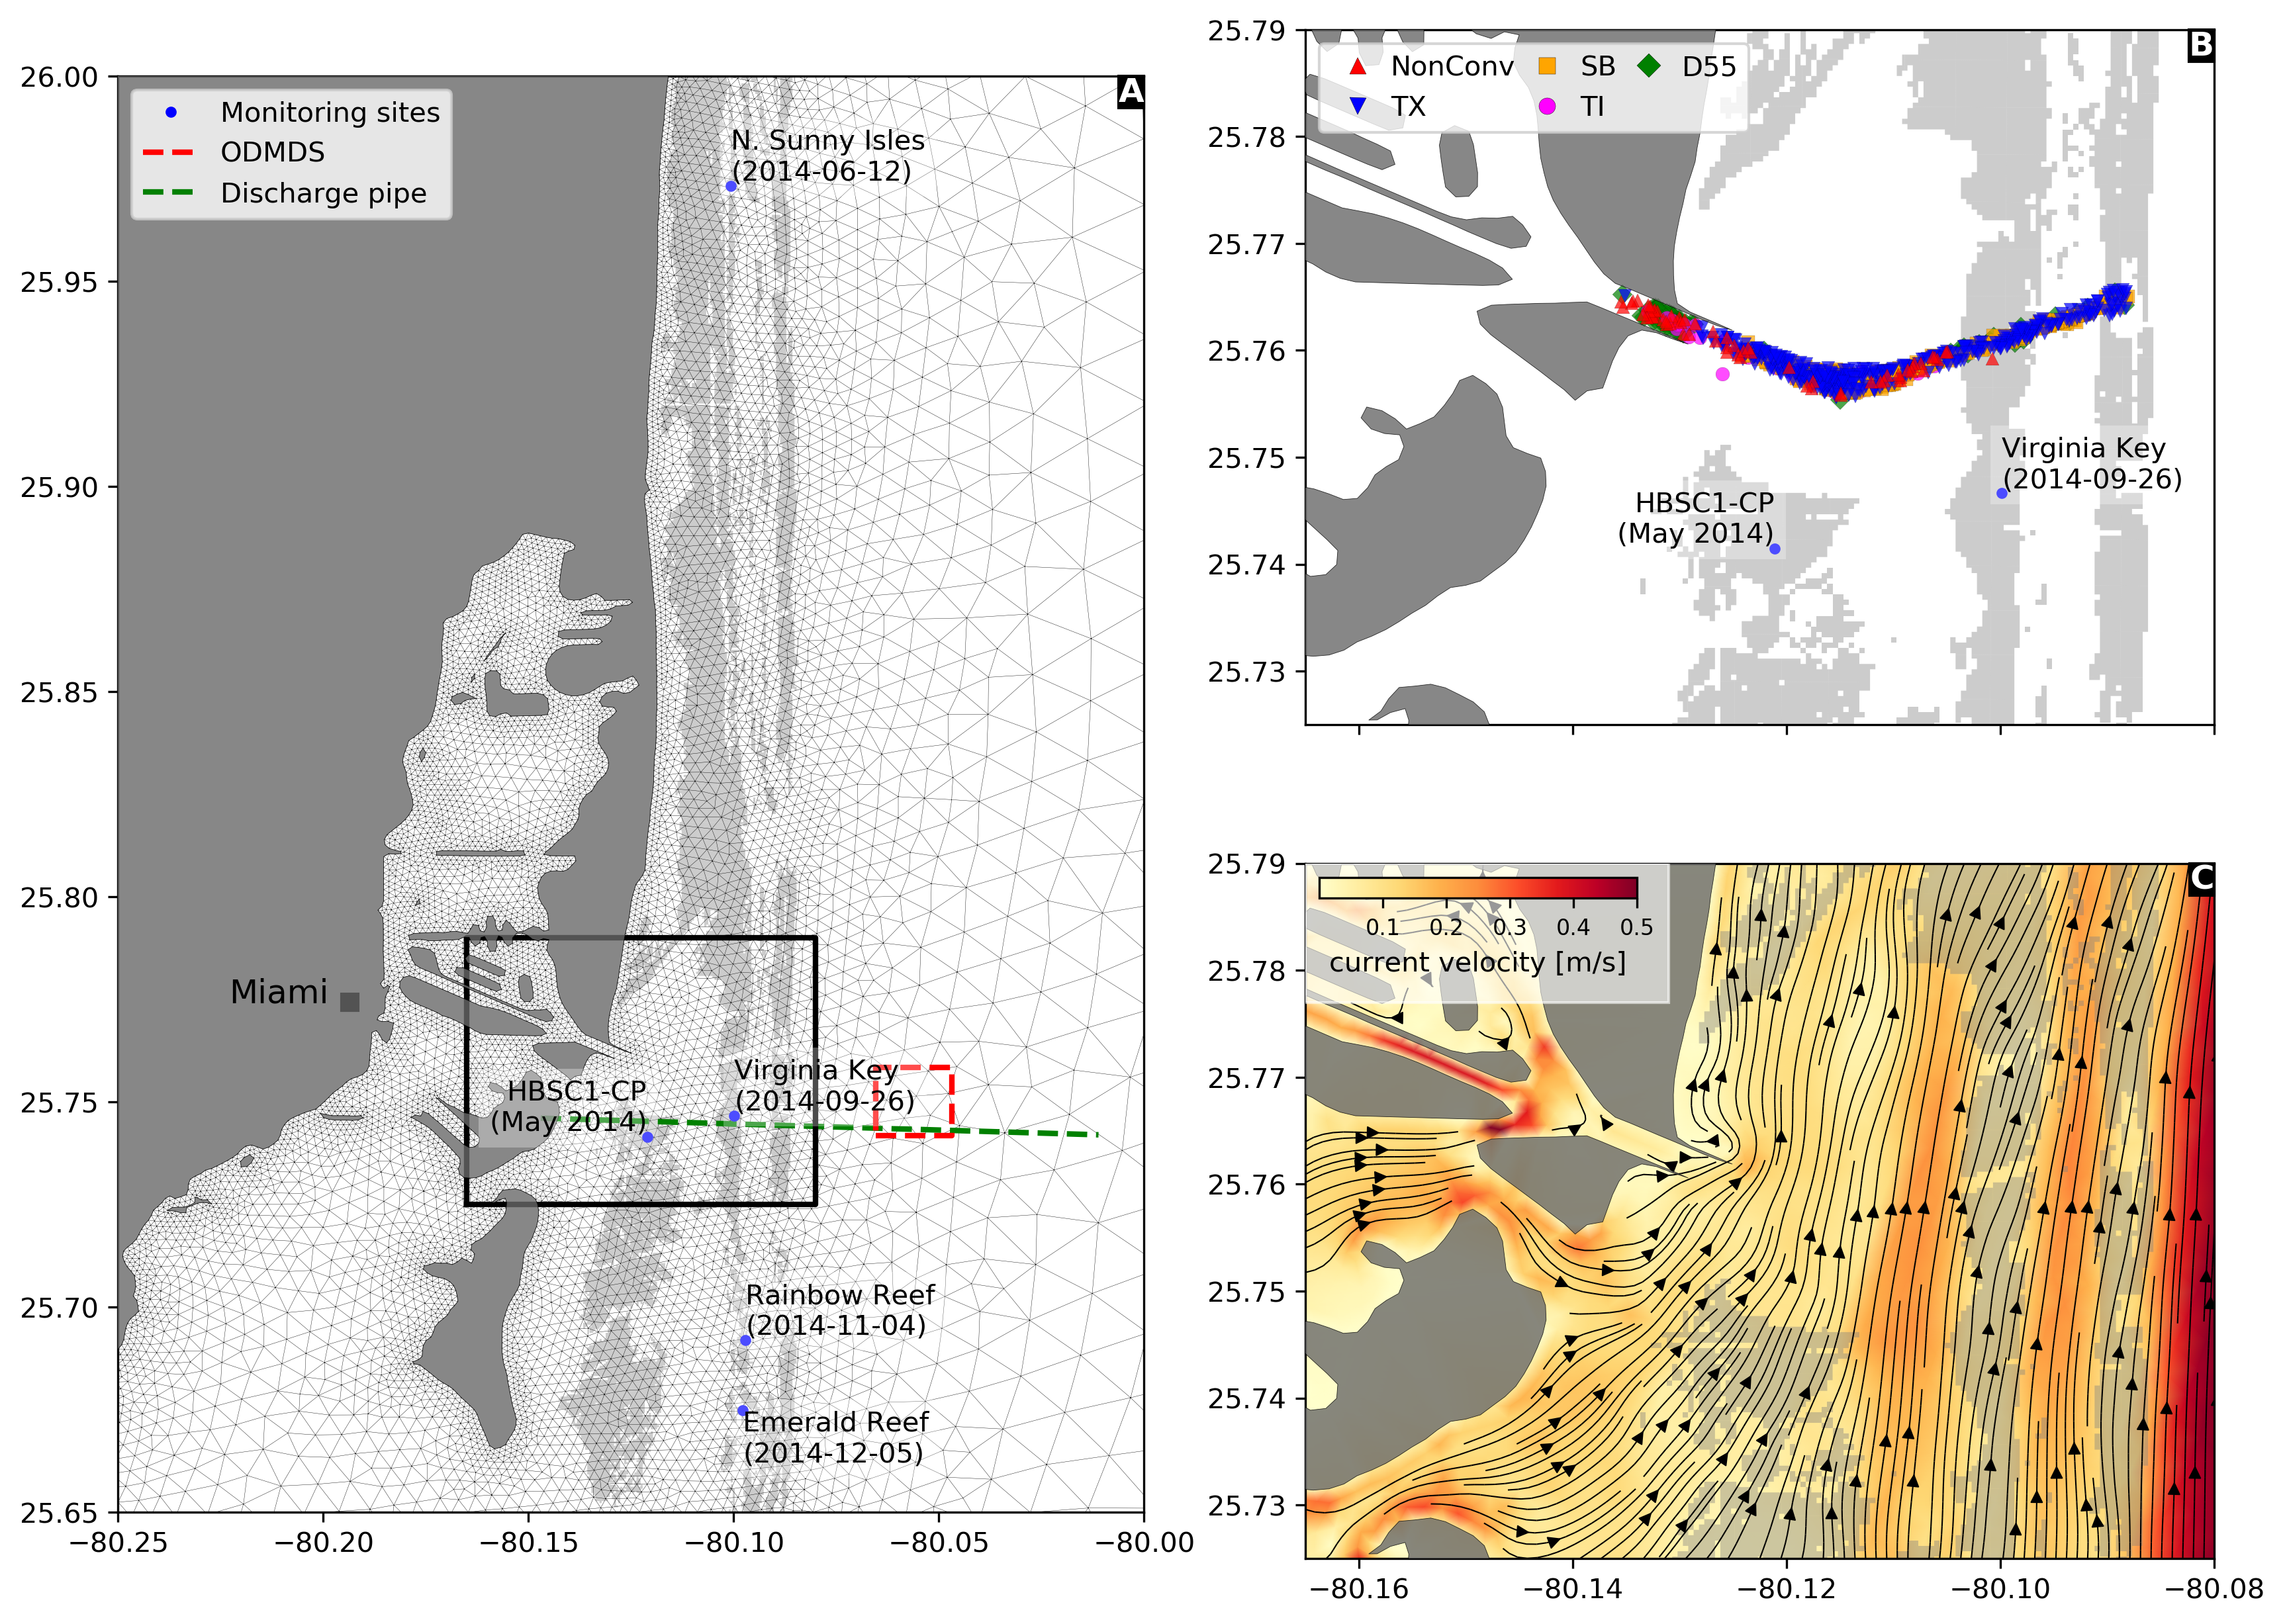
\includegraphics[width=\textwidth]{chapters/onset/figures/fig_mesh_onset.png}
	\caption{\textbf{A}: Model mesh near the dredged channel. Elements have a characteristic length of 100 m over reefs (in light grey) and along the coasts (in dark gray). The monitoring sites considered in the present study are shown by blue dots. The date where SCTLD was first observed at these sites is given between brackets. The Ocean Dredge Material Disposal Site (ODMDS) is shown in red and the discharge pipe of the Miami Central District Municipal Wastewater Treatment Plant in green. \textbf{B}: Close up view of the dredged channel. The locations of the different types of dredging that took place during the expansion of PoM are shown by colored markers. \textbf{C:} Snapshot of the modeled currents in the vicinity of the dredged channel. Small-scale flow features such as the acceleration of currents between reefs and islands are well reproduced by the model.}
	\label{fig:onset_mesh}
\end{figure}

The hydrodynamics of the entire FCR was modeled using the multi-scale ocean model SLIM\footnote{\url{ https://www.slim-ocean.be}}, which has already been extensively validated in the area \citep{frys20,dobbelaere2020coupled,dobbelaere2022}. SLIM uses an unstructured mesh whose resolution can be locally increased in order to accurately represent fine-scale flow features. The mesh used in this study was built following the same methodology as \cite{dobbelaere2022}, with a local refinement near PoM and in the Bay of Biscayne to achieve a resolution of 100 m in the vicinity of the dredged channel (Fig. \ref{fig:onset_mesh}A). It was made up of approximately $3.5\times 10^5$ triangles and was generated with the seamsh\footnote{\url{https://pypi.org/project/seamsh/}} Python library, which is based on the the open-source mesh generator GMSH \citep{geuzaine2009gmsh}. The model was run between October 15, 2013 and September 26, 2014 to cover the whole dredging period prior to the first observation of SCTLD by \cite{precht2016unprecedented}. Figure \ref{fig:onset_mesh}C depicts how a 100-m spatial resolution mesh simulated fine-scale details of the ocean currents, such as the flow acceleration between reefs and islands.

The transport of sediments released from the channel was then modeled using a Lagrangian particle tracking model, forced by the simulated currents. The sediment model is inspired by the Particle Transport Model (PTM), developed by the US Army Corps of Engineers \citep{macdonald2006ptm}. In this model, particles undergo a combination of horizontal and vertical motions. The vertical is mostly driven by gravity, with heavier particles sinking faster. Once they have settled, particles can be resuspended when shear stress exceeds   the critical Schields parameter, as parameterized by \cite{soulsby1997threshold}. The horizontal motion of the suspended particles is derived from the 2D model velocity by assuming a vertical log profile, hence yielding a quasi-3D approach. When sediment particles enter the near-bed zone, their horizontal velocity is greatly reduced and sediments are transported with the bedload.   

As sediment dispersion is dependent on the grain size, we modeled the dispersal of five sediment classes to represent to impact of fine- to coarse-grained particles: ($i$) 5-50 $\mu$m, ($ii$) 50-100 $\mu$m, ($iii$) 100-200 $\mu$m, ($iv$) 200-300 $\mu$m, and ($v$) 300-400 $\mu$m. We performed a  different simulation for each class, with the grain size randomly drawn from a uniform distribution over the corresponding size range. The density of each sediment particle was derived from their size using the formula of \cite{hamilton1982sound}. Furthermore, all particles were differentiated based on the type of dredge that produced them. Five types of dredge were considered in our modeling study (Fig. \ref{fig:onset_mesh}B): ($a$) Texas cutterhead (TX), ($b$) non-conventional dredging, \ie TX with suction mechanism turned off (NonConv), ($c$) Spider Barge (SB), ($d$) Terrapin Island hopper (TI), and ($e$) Dredge 55 clamshell (D55).

Dredging operations performed during the expansion of PoM were characterized in our dataset by a date, a location and  a type of dredging operation (Fig. \ref{fig:onset_mesh}B). In the absence of information about the exact time of the dredging, sediment particles were released from the dredging location during a whole day at a rate of 80 particles/hour in the model. To account for the motion of spider barges between the dredging site and disposal site, particles were released every 500 m along a straight line joining the dredging location to the ODMDS (see Fig. \ref{fig:onset_mesh}A) for every dredging operation labelled as SB.

The outputs of the sediment model were then used to evaluate the turbidity and sedimentation generated by the expansion of PoM over coral reefs. The occurrence of high turbidity over reefs was assessed based on the concentration of suspended sediment particles in the model. This concentration was computed by counting the number of suspended particles inside the cells of a regular 200 m $\times$ 200 m grid over our computational domain. The modeled occurrence of plume was then compared against daily data of plume detection. This dataset was derived from satellite imagery by \cite{cunning2019extensive}\footnote{datasets available at \url{https://github.com/jrcunning/pom-dredge/}} following the methods of \cite{barnes2015sediment} at sites located within 15 km of the dredged channel. As in these two previous studies, we computed  the simulated plume frequency by dividing the number of days during which plumes occurred by the total number of simulated days for all grid cells. The impact of sedimentation was quantified by computing the cumulated concentration of settled particles within the same computational grid. This cumulated concentration was normalized by the total number of simulated time steps to obtained an averaged concentration of deposited particles over the simulated period. Higher values of this indicator would indicate larger sediment deposition over longer cumulated time.

The potential impact of dredging on the onset of the SLD outbreak was more specifically assessed at five monitoring sites were signs of disease were reported. Four sites were reefs where disease was reported in 2014 by \cite{precht2016unprecedented}. The fifth site was monitoring station HBSC1-CP of the monitoring of the expansion of PoM, where signs of disease were already reported in May 2014 (Fig. \ref{fig:onset_mesh}A, see pictures in Appendix). The impact of dredging was assessed by counting the number of sediment particles originating from each dredging that were transported within 500 m of all five site. This distance was chosen to match the scale of the 500 m $\times$ 500 m reef polygons used in the model \citep{dobbelaere2020coupled}. The obtained number of particles was then divided by the total number of sediment particles released by each type of dredge. Larger values of this indicator would suggest a greater impact of a given type of dredging operation at a given monitoring sites.  

Finally, as previous studies showed evidence of waterborne transmission of SCTLD \citep{aeby2019pathogenesis, dobbelaere2020coupled,eaton2021measuring, meiling2021variable}, there is a possibility that the disease propagated to Virginia Key from other diseased reefs affected prior to September 2014. To evaluate this possibility, we computed monthly disease connectivity matrices following the methodology of \cite{dobbelaere2020coupled} during our simulated period. These connectivity matrices can be interpreted as large graphs whose vertices are 500 m $\times$ 500 m reef areas and whose edges represent disease connectivity pathways. Evaluating the possibility of disease propagation from any sub-reef $A$ to any sub-reef $B$ is therefore equivalent to evaluating the existence of paths, \ie sequences of connected vertices in the network starting from $A$ and reaching $B$. As computing all possible paths is not computationally tractable, we limited ourselves to the computation of shortest paths from any given reefs to the Virginia Key monitoring site. This was performed using the function \texttt{get\_all\_shortest\_paths} of the Python \texttt{python-igraph} package \citep{csardi2006igraph}. Such function requires the definition of a weight $w_{ij}$ for the edge connecting reef $i$ to reef $j$. We chose $w_{ij} = 1-\tilde{C}_{ij}$, where $\tilde{C}_{ij}$ is the probability of disease propagation from reef $i$ to reef $j$, so that "shorter" edges of the networks (\ie connectivity pathways with smaller weights) correspond to connections with larger disease propagation probability. The probability of a given path was then defined as the mean connection probability of the edges composing this path.

Finally, the 2D mode of the particle tracking model was used to assess the impact of wastewater leaking from the discharge pipe mentioned by \cite{gintert2019regional}. This model simulates the transport of neutrally buoyant material driven by mean current within the water column \citep{dobbelaere2020coupled}. Without clear information about the location of the leak, particles were continuously released every 100 m along a straight line between Miami Central District Municipal WWTP, located on Virginia Key and the ocean discharge outfall located at 25$^\circ$44'31''N 80$^\circ$05'10''W \citep{koopman2006ocean}. The impact of wastewater released from the different potential leak locations was then evaluated by computing the fraction of released wastewater particles that were transported within 500 m of the site of Virginia Key.

%%%%%%%%%%%%%%%%%%%
% --- RESULTS --- %
%%%%%%%%%%%%%%%%%%%
\section{Results}

5-50 $\mu$m was the only grain size that produced plumes consistent with the observations of \cite{barnes2015sediment} and \cite{cunning2019extensive} (Fig. \ref{fig:onset_depo}A). For larger grain sizes, particles settled in the direct vicinity of the channel. For these heavier particles, suspended sediments were only observed offshore, closer to the Florida Current, where the current velocity was sufficiently strong to prevent deposition. This suggests that the observed turbidity was mostly due to fine silts. The modeled occurrence of plumes within 15 km of the dredged matched the presence/absence data of \cite{cunning2019extensive} in 82.7\% of cases and the total area where plumes were observed was about 230 km$^2$, consistent with the $\sim228$ km$^2$ estimated by \cite{barnes2015sediment}. Modeled plumes mostly occurred north of the dredged channel, as particles were driven northward under the action of the Florida Current, with plume frequencies of about 20\% near the monitoring site of N. Sunny Isles. Plume frequencies was lower ($\sim 5$\%) over offshore reefs but reached of up to 50\% over alongshore reefs. These alongshore reefs correspond to regions of important sedimentation (Fig. \ref{fig:onset_depo}B), which is consistent with the correlation between plumes and sedimentation highlighted in \cite{cunning2019extensive}. The plume frequency was about 1\% at site of HBSC1-CP while no plume occurred at other southern monitoring sites during the simulation. 

% \begin{table}
	%     \centering
	%     \begin{tabular}{|l|cccc|}
		%         \hline
		%          & Threshold         & Accuracy & False positive  & False negative \\
		%          & [particles/m$^2$] & [\%]     & [\%]            & [\%]  \\
		%         \hline
		%         5-50 $\mu$m    & 21 & 86.678 & 2.912 & 10.410 \\
		%         50-100 $\mu$m  & 20 & 83.058 & 8.525 & 8.417 \\
		%         100-200 $\mu$m & 30 & 84.814 & 7.133 & 8.053 \\
		%         200-300 $\mu$m & 18 & 84.459 & 7.988 & 7.553 \\
		%         300-400 $\mu$m & 13 & 84.615 & 8.140 & 7.244 \\
		%         \hline
		%     \end{tabular}
	%     \caption{Validation of the modeled presence of plumes against plume observations from satellite imagery. Overall, the model agrees well with observations}
	%     \label{tab:onset_val} 
	% \end{table}

\begin{figure}
	\centering
	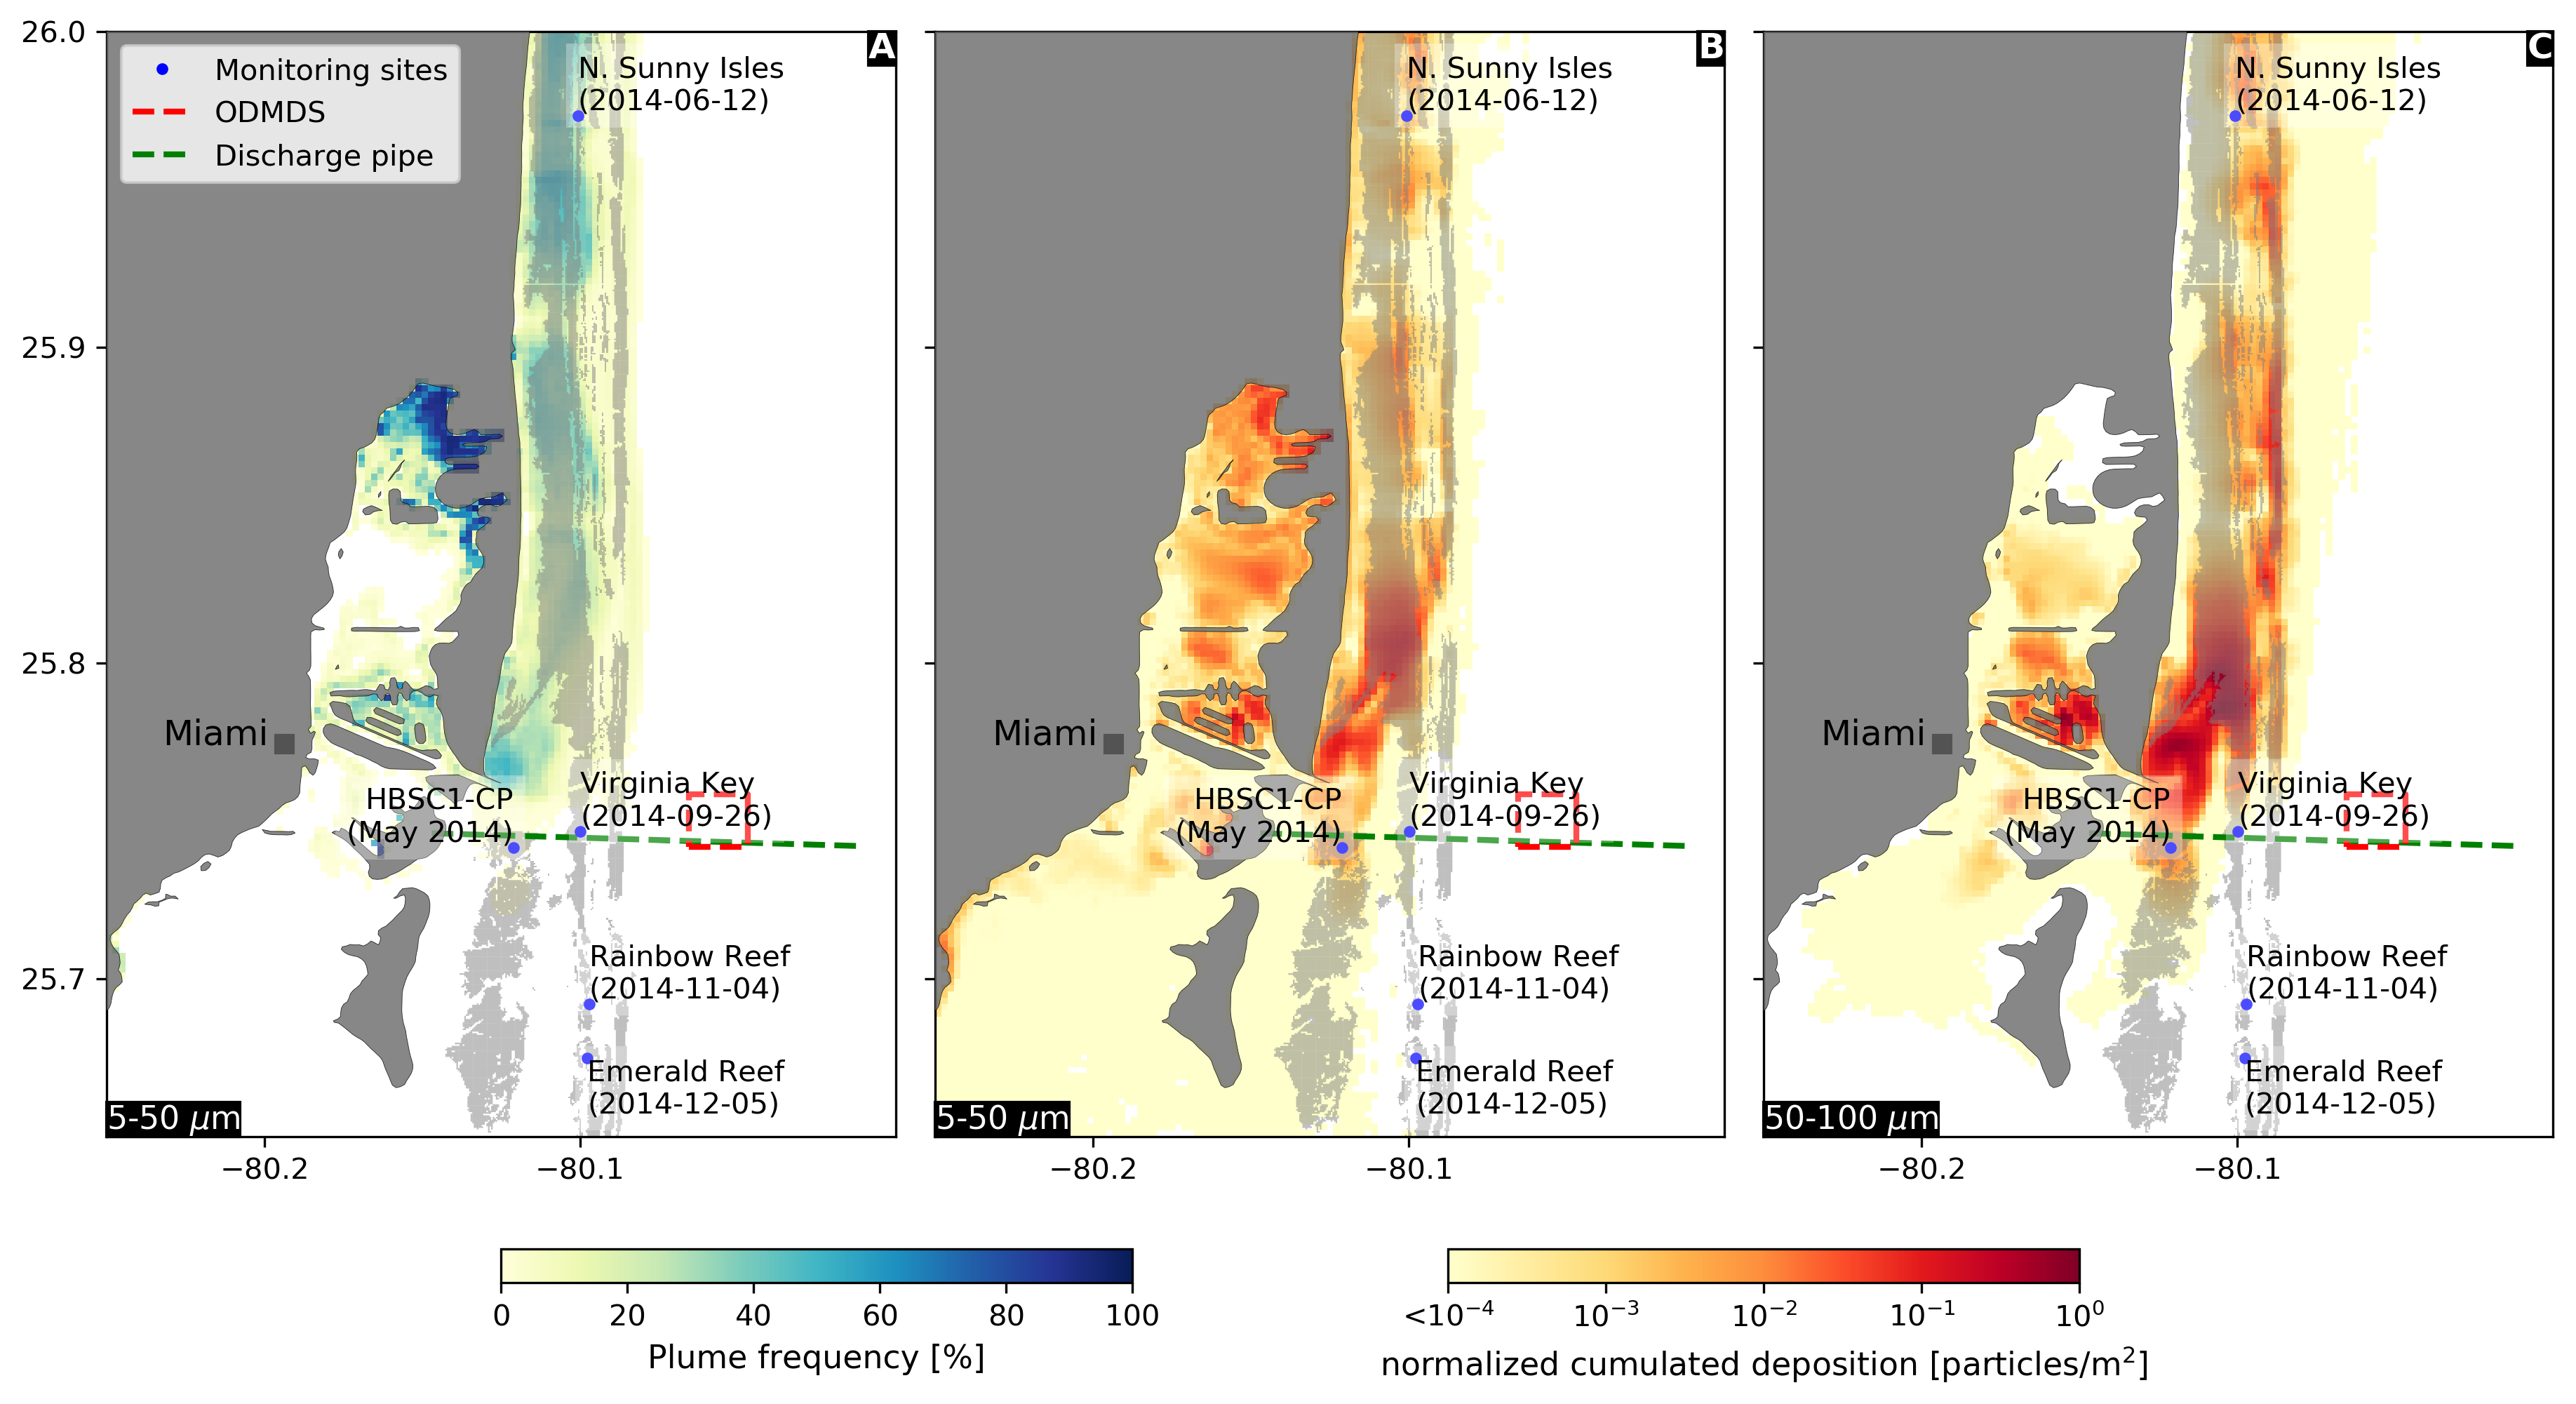
\includegraphics[width=\textwidth]{chapters/onset/figures/deposition_plumes.png}
	\caption{\textbf{A}: Plume frequency for grain size in the range 5-50 $\mu$m. The averaged concentration of deposited sediments are shown for grain sizes more likely to carry the disease: 5-50 $\mu$m (\textbf{B}) and 50-100 $\mu$m (\textbf{C}). Most modeled turbidity and sedimentation occurred north of the dredged channel. Non negligible sediment deposition occurred at site HBSC1-CP.}
	\label{fig:onset_depo}    
\end{figure}

Deposition results are shown for grain sizes corresponding to silts, which are more likely to carry organic matter and therefore more likely to carry SCTLD agents \citep{erftemeijer2012environmental}(Fig. \ref{fig:onset_depo}B,C). Sedimentation mostly occurred on reefs located north of the dredge channel. For grain sizes smaller than 5-50 $\mu$m, sediments mostly settled on inshore reefs while sedimentation mostly took place on offshore reefs for grain size larger than 50$\mu$m. When increasing grain sizes, the spatial distribution of sedimentation shifted southward, with a decrease of sedimentation near N. Sunny Isles and an increase of the concentration of settled sediments near HBSC1-CP and Virginia Key. The normalized cumulated deposition was around 0.01 particles/m$^2$ at site HBSC1-CP for all grain sizes while it increased from $2.5\times 10^{-7}$ to $1.6\times 10^{-3}$ with grain size at Virginia Kay. For all grain sizes, no sedimentation occurred near Rainbow Reef and Emerald Reef. However, sediments settled at similar latitudes west to these sites for grain sizes below 100 $\mu$m.

The evaluation of the impact of dredging at the monitoring sites indicated that dredging did not significantly impact the stations located south of the dredge channel, except at site HBSC1-CP (Fig. \ref{fig:onset_bar}). In contrast, up to 40\% of the released sediment particles reached the northern site of N. Sunny Isles. The impact of dredging at this site decreased with sediment size and the fraction of sediment particles reaching the N. Sunny Isles dropped below 2\% for grain sizes larger than 200 $\mu$m. However, for grain sizes finer than 50 $\mu$m, N. Sunny Isles was heavily impact by TX dredging. Indeed, the number of particles produced by TX reaching N.Sunny Isles was 50\% larger than the cumulated number of particles produced by other dredging operations reaching the monitoring site for the same grain size. Such large impact can be explained by the fact that TX was one of the most frequent type of dredging during the simulations, with 268 simulated operations (Fig. \ref{fig:onset_bar}C). However, SB events occurred at an equivalent frequency but resulted in 4 times fewer particles to reach N. Sunny Isles. For grain sizes below 100 $\mu$m, between 10\% and 30\% of the sediments released by non conventional dredging reached N. Sunny Isles. This fraction dropped below  1\% for grain sizes larger than 200$\mu$m. The fraction of sediments produced by non conventional dredging reaching site HBSC1-CP remained between 1\% and 5\% for all grain sizes. For grain sizes below 100 $\mu$m, D55 and NonConv were the main sources of sediments reaching HBSC1-CP. Above 100 $\mu$m, the main source of sediments to the site became TI. The fraction of sediments produced by SB reaching HBSC1-CP remained negligible for all grain sizes. No sediment particles reached the sites of Rainbow Reef and Emerald Reef for all grain sizes. However, some particles reached Virginia Key for grain sizes larger than 100 $\mu$m. These sediments particles almost entirely originated from SB. Nonetheless, the impact of the dredging on Virginia Key remained limited with less than 1$\%$ of the released particles reaching the site.

\begin{figure}
	\centering
	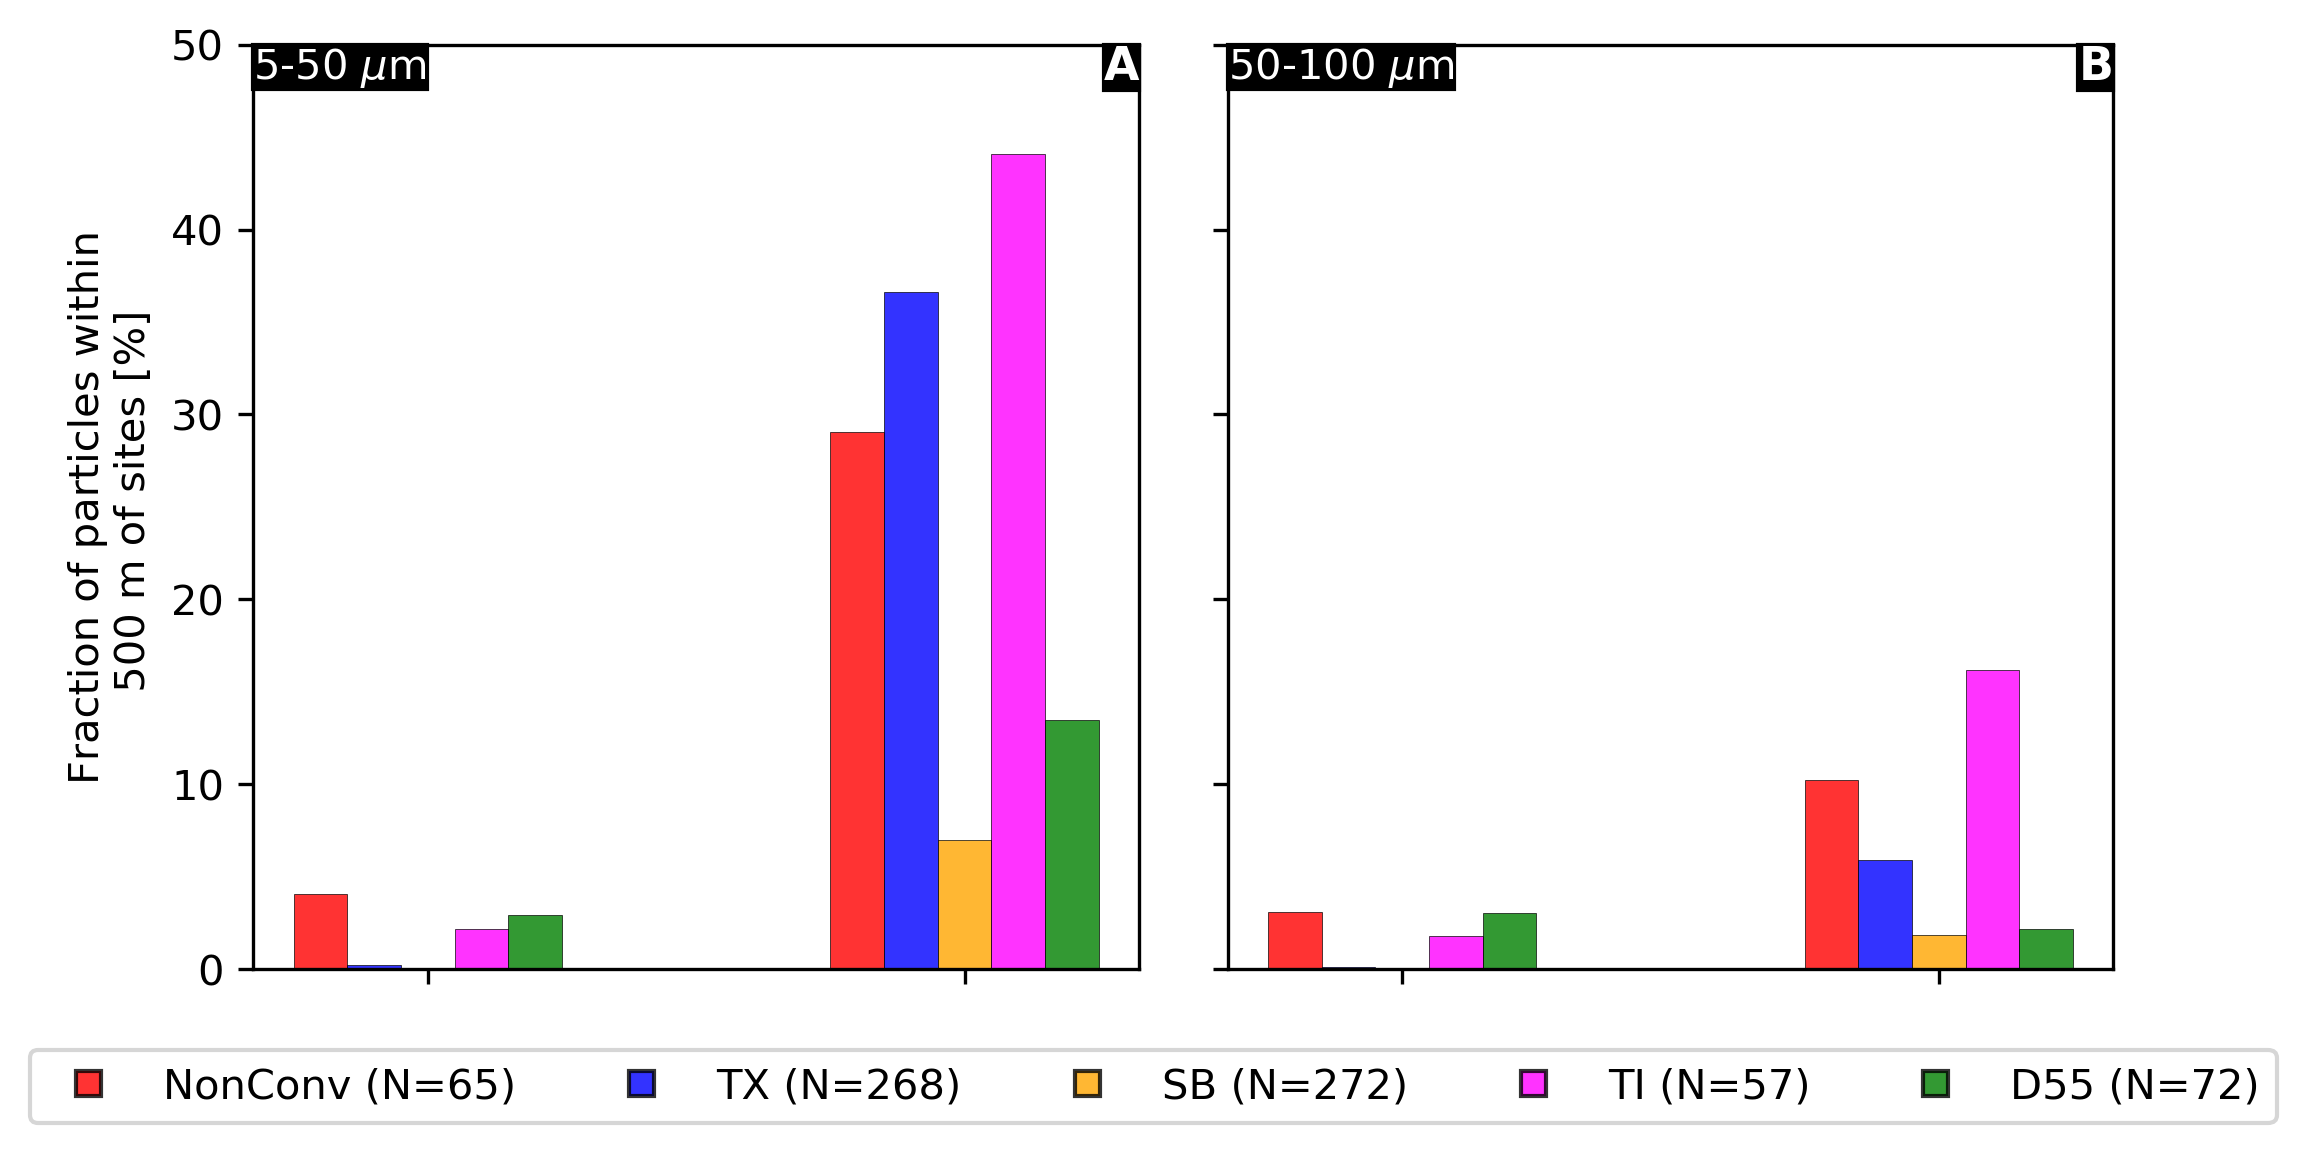
\includegraphics[width=\textwidth]{chapters/onset/figures/aggregated_new.png}
	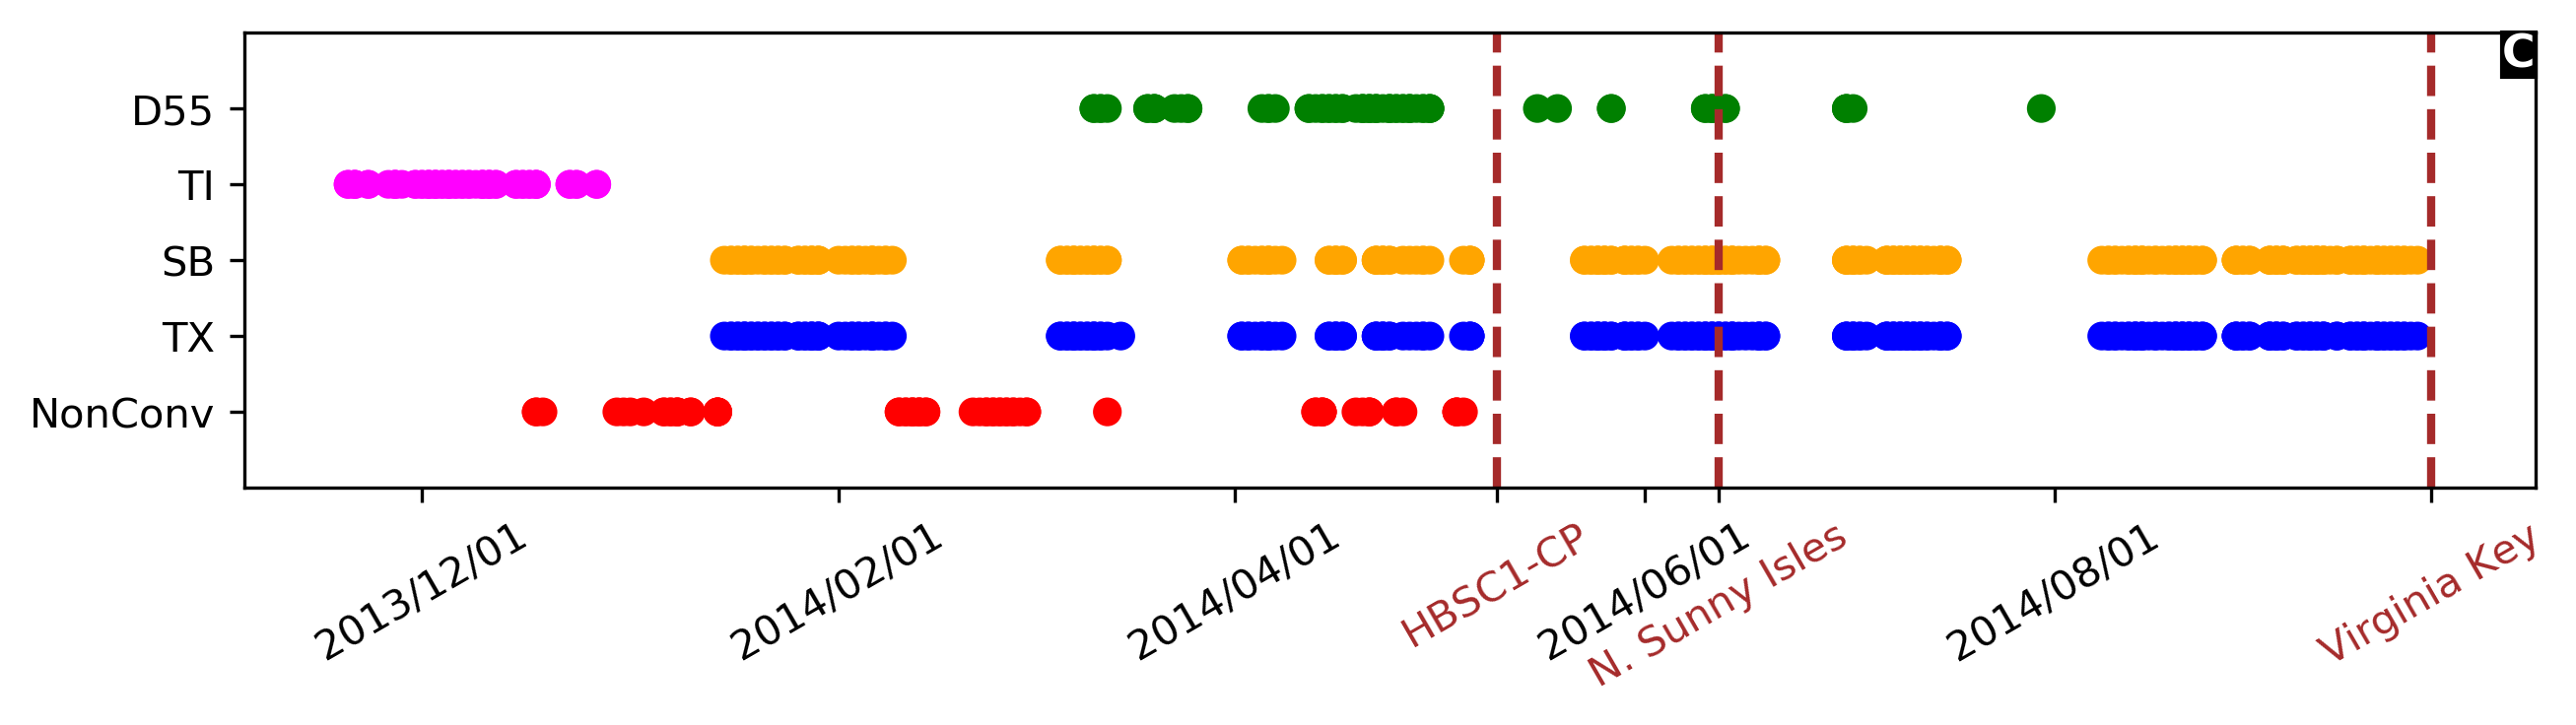
\includegraphics[width=\textwidth]{chapters/onset/figures/timeline.png}
	\caption{Fraction of sediment particles released by each type of dredge that drifted within 500 of HBSC1-CP and N. Sunnny Isles with grain sized of 5-50 $\mu$m (\textbf{A}) and 50-100 $\mu$m (\textbf{B}). \textbf{C}: Temporal distribution of the simulated dredging operations. The dates of the first reported disease signs at each monitoring site are shown in brown. With the exception of HBSC1-CP, sites located south to the dredged channel were barely impacted by the dredging. However, a significant fraction of the released sediment particles reached the northern site of N. Sunny Isles. The number of simulated dredging operations is given between brackets for each dredging type}
	\label{fig:onset_bar}
\end{figure}

Applying the same analysis to the discharge pipe of Miami Central District Municipal WWTP suggests that only wastewater released from a leak in the direct vicinity of the Virginia Key could have impacted the site. Fig. \ref{fig:onset_pipe} shows the fraction of released wastewater particles that reached the site of Virginia key for every 100 m segments of the discharge pipe. The fraction of particles that drifted within 500 m of Virginia Key was: 100\% for particles released within 500 m of the site; 0-1\% for particles released between 500 m and 1.5 km away from the site; and 0\% for all other sources of wastewater particles. As HBSC1-CP was also located near the discharge pipe, a similar analysis was conducted for this monitoring site and gave similar results.

\begin{figure}
	\centering
	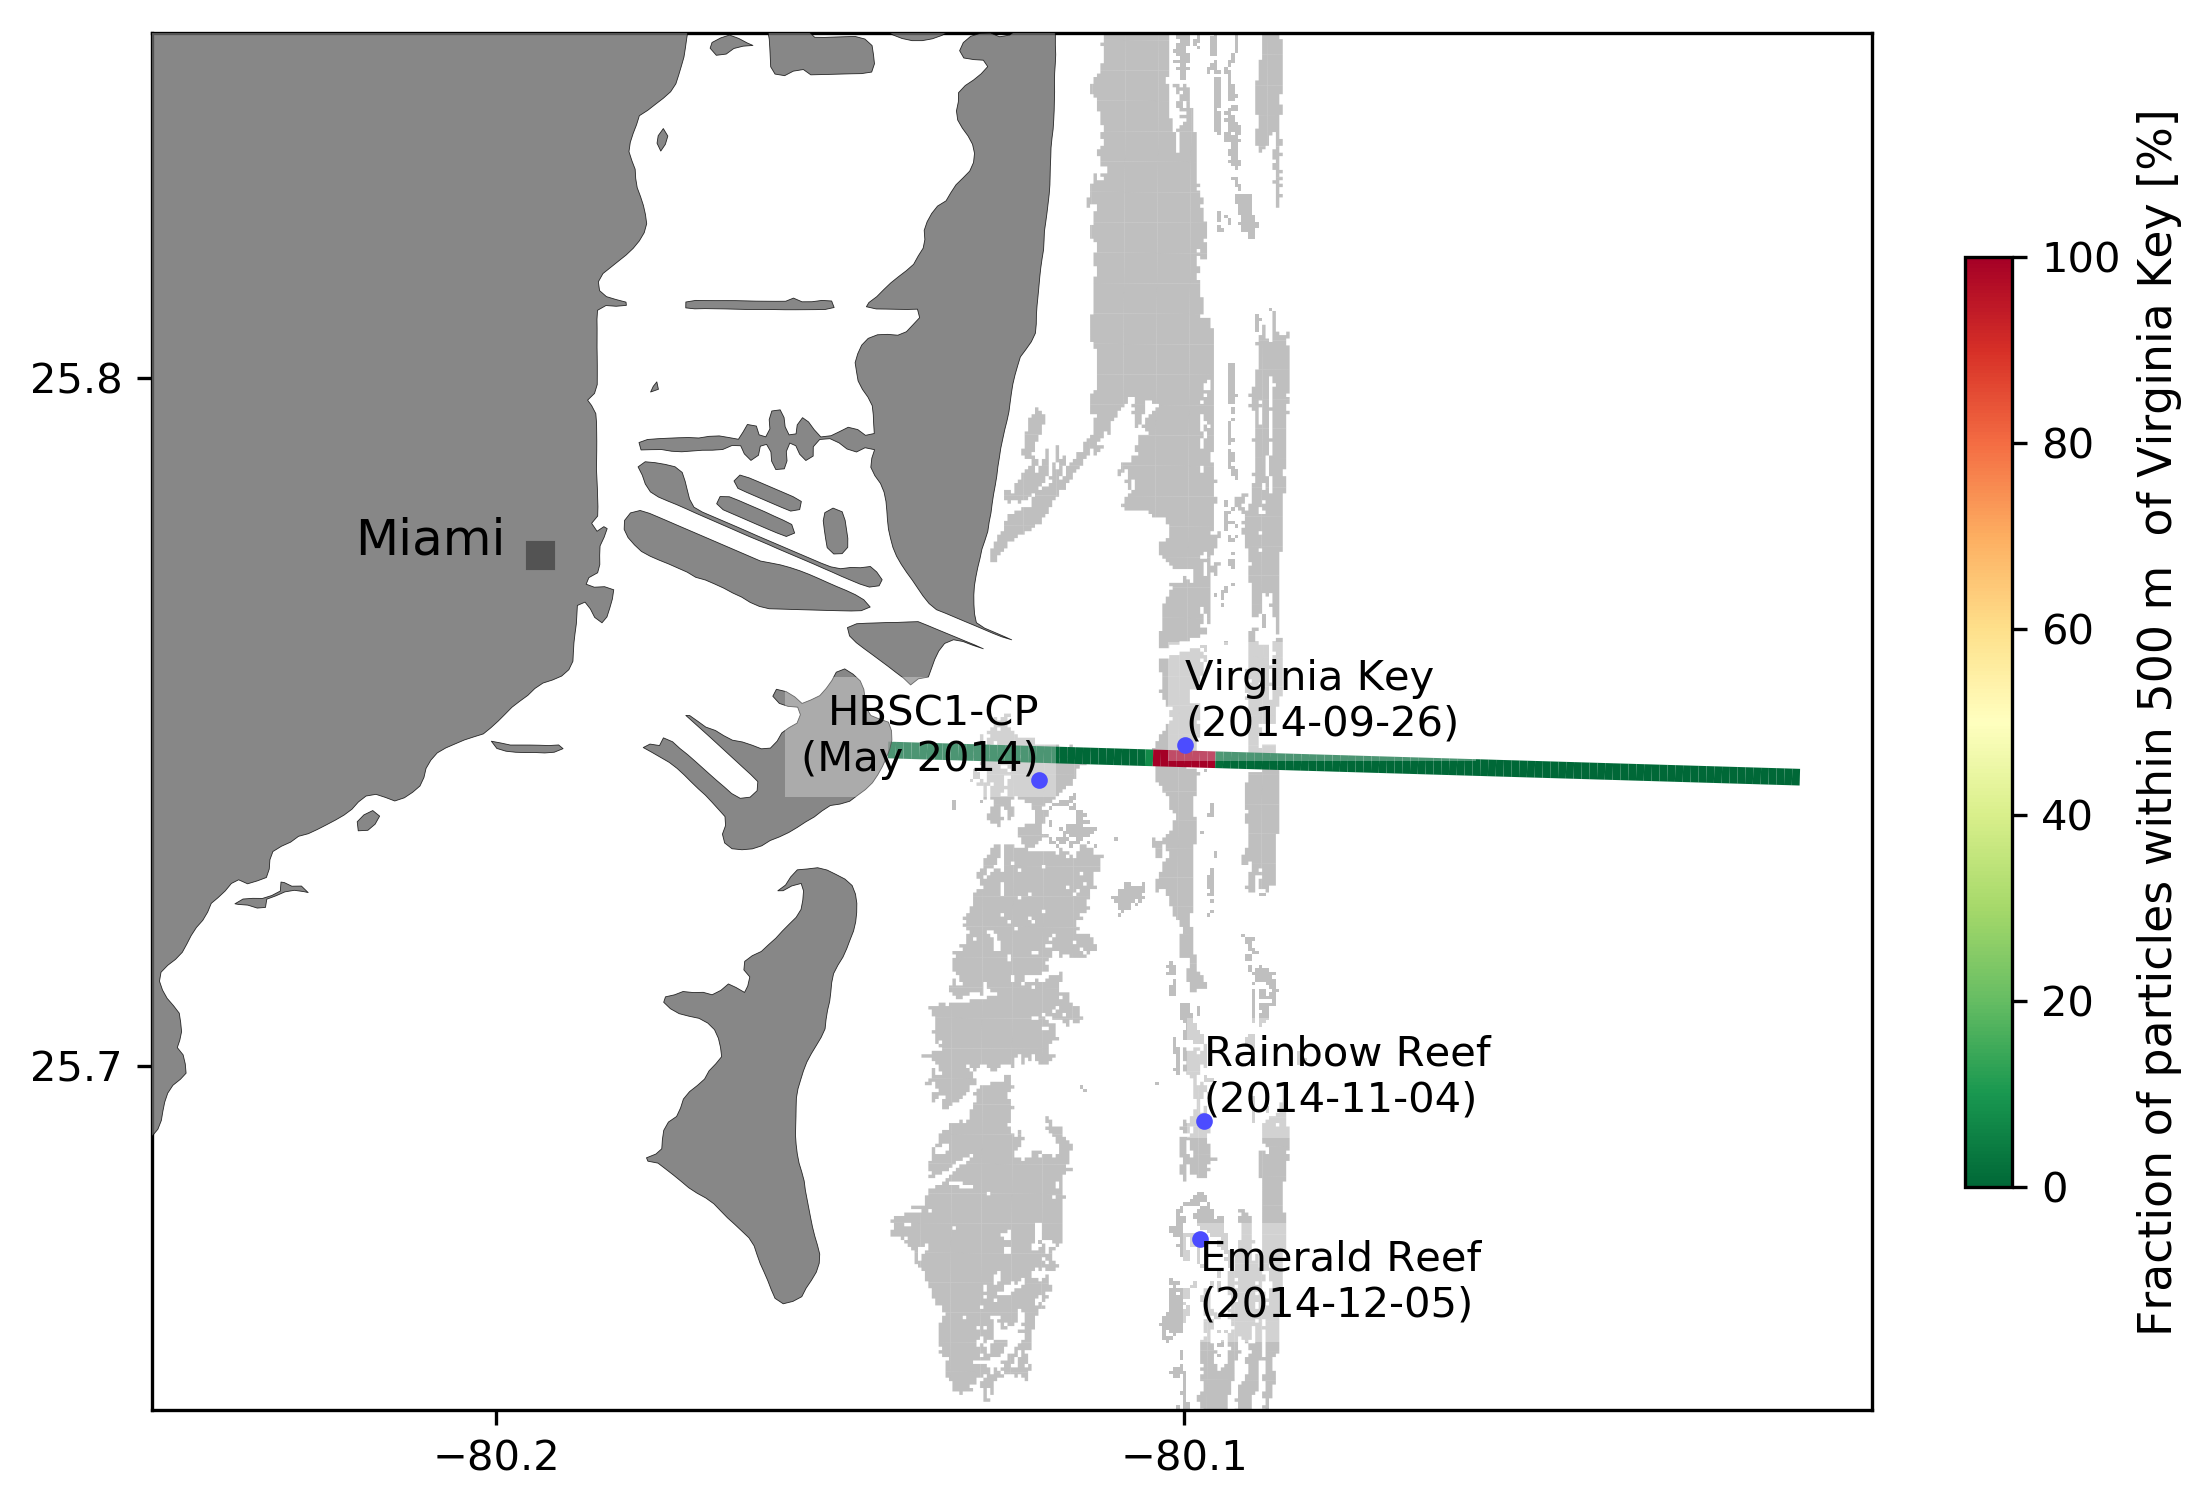
\includegraphics[width=.7\textwidth]{chapters/onset/figures/pipeline.png}
	\caption{Fraction of wastewater particles reaching the site of Virginia Key for potential leak positions located every 100 m along the discharge pipe. Only particles released in the direct vicinity of Virginia Key could reach the monitoring site.}
	\label{fig:onset_pipe}
\end{figure}

As signs of disease were observed at site HBSC1-CP in May 2014, before the first observations of SCTLD in Virginia Key in September 2014, we assessed the presence of shortest paths from HBSC1-CP to Virginia Key in the modeled monthly disease connectivity networks between May and September 2014 (Fig. \ref{fig:onset_path}). We found connectivity pathways connecting the two sites during all months of May-September 2014, with the exception of July. This suggests that there was a possibility of disease propagation from HBSC1-CP to Virginia Key during most of these 5 months. However, we found no direct pathway connecting the two sites. Southern intermediary reefs were systematically needed as stepping stones for the propagation of the disease. This suggests that several months might have been required for disease agents to reach Virginia Key from HBSC1-CP. Moreover, shortest paths in June, August and September 2014 had many sub-reef stepping stones in common. These similar connectivity patterns indicate favorable conditions for disease propagation over several months from HBSC1-CP to Virginia Key during this period.  

\begin{figure}
	\centering
	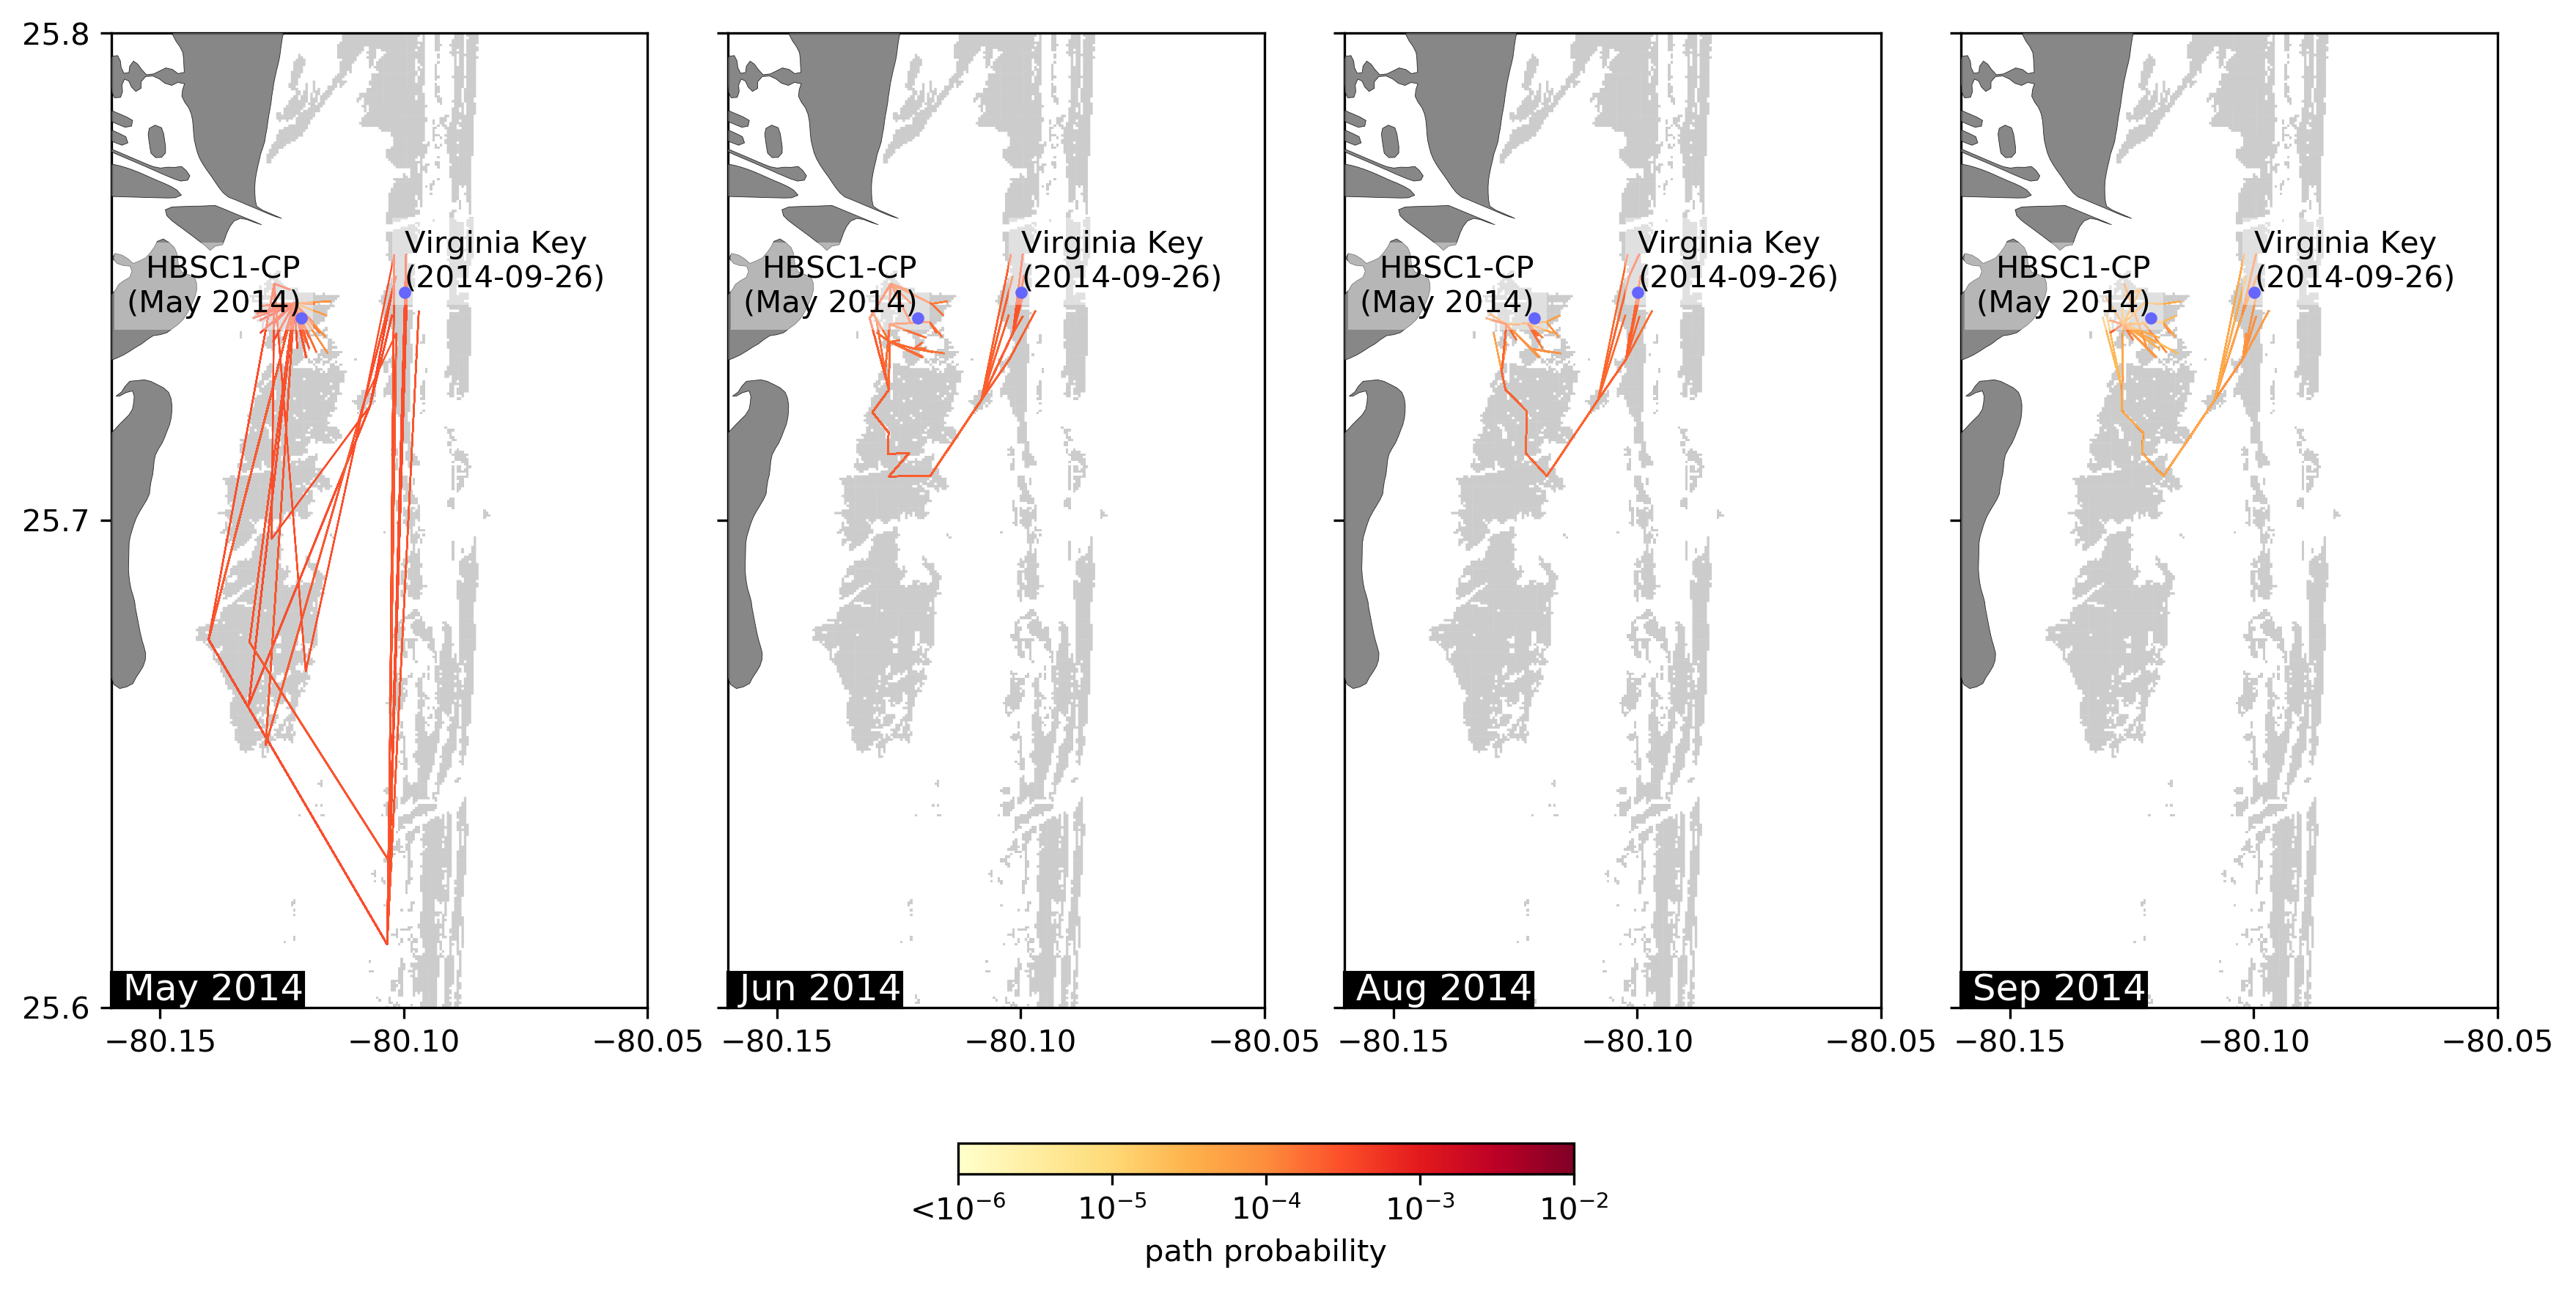
\includegraphics[width=\textwidth]{chapters/onset/figures/fig_paths.png}
	\caption{Shortest path from HBSC1-CP to Virginia Key in the monthly disease connectivity networks between May and September 2014. July 2014 was the only month without modeled connectivity between the two sites between May and September 2014. Southern intermediary reefs were needed as stepping stones for the propagation of the disease from HBSC1-CP to Virginia Key.}
	\label{fig:onset_path}
\end{figure}

% === DISCUSSION === %
\section{Discussion}

% SUMMARY
The quasi-3D sediment model forced by currents from the high-resolution coastal ocean model SLIM reproduced a sediment dynamics consistent with plume observations derived from satellite imagery. It suggests that sediment particles produced by dredging were mostly transported northward under the influence of the Florida Current. No sediment particles reached the southern sites of Rainbow Reef and Emerald Reef while dredging had limited direct impact on Virginia Key, identified as the site where the outbreak of SCTLD was initiated in September 2014. Furthermore, our results indicate that it is unlikely that the site was affected by a leaking discharge pipe of Miami Central District Municipal WWTP, as suggested by \cite{gintert2019regional}. However, signs of disease were observed prior to September 2014 at the sites of N. Sunny Isles and HBSC1-CP, where the impact of dredging was greater. Up to 30\% of silt particles produced by non-conventional dredging reached coral reefs of N. Sunny Isles while 5\% of them reached site HBSC1-CP, where significant sedimentation occurred. Furthermore, analysis of monthly disease connectivity networks indicate disease transmission from HBSC1-CP to the site of Virginia Key was possible through waterborne transmission.   

% LARGE IMPACT OF DREDGING
Our study confirms previous reports about the widespread impact of the expansion of PoM. As in \cite{barnes2015sediment}, the total area of plumes in our model was about 230 km$^2$. Furthermore, the model results reproduced the presence/absence within 15 km of the dredged channel derived by \cite{cunning2019extensive} with an accuracy of 82.7\%. Such good agreement was only obtained for grain sizes in the range 5-50 $\mu$m, suggesting that fine silts were the main drivers of the turbidity generated by dredging, which is consistent with previous studies \citep{fourney2017additive}. Despite this good agreement, the distribution of plumes predicted by our model tends to be shifted northward compared to these previous studies. These discrepancies might be explained by the fact that our approaches is solely based on sediment concentration. However, turbidity depends on many local factors such as the water content of phytoplankton and organic matters \citep{gray2000comparability,thackston2000improved}. As reported by \cite{cunning2019extensive}, the plumes mostly occurred in areas of high sedimentation. As such areas were mostly located over coral reefs, our results suggests that the expansion of PoM might have harmed coral populations over an extended area through increased turbidity and sedimentation. This sedimentation mostly took place on alongshore reefs for grain sizes smaller than 50$\mu$m and on offshore reefs for coarser grain sizes. Sediment settlement might be significantly harmful to offshore coral reefs populations as they are usually less accustomed to sedimentation than their inshore  counterparts \citep{wolanski2005fine}.

% LIMITATION + SHOW THAT N. SUNNY ISLE AND HBSC1-CP WERE SIGNIFICANTLY IMPACTED
A limitation of our study is that the amount of released sediments might be overestimated, as conventional and non-conventional dredging are treated in the same way in the model. For all dredging types, sediment particles were released at the same rate in the model. Although conventional dredging was reported to release fine-grained sediments in the water column through dewatering and overflow from barges \citep{jones2016assessing}, the quantity of dredged material lost in the water was limited by the use of pumping mechanisms. By contrast, for non-conventional dredging, the suction mechanism was turned off, causing all chopped rock particles to be released in the water column. The numbers of particles reaching the monitoring sites were therefore likely overestimated for all sources but non conventional dredging. However, the fractions given in Fig. \ref{fig:onset_bar}A,B remain valid as they are relative to the total number of sediments released in the water columns. Despite these overestimations, the coral reefs of N. Sunny Isles appeared to be highly sensitive to fine-grained sediments produced by dredging (Fig. \ref{fig:onset_bar}). Furthermore, the non-conventional rock-chopping that took place between December 2013 and May 2014, was a non-negligible source of sediments to N. Sunny Isles, as up to 30\% of the released particles reached the site. As sediments have the potential to act as a SCTLD vector \citep{rosales2020rhodobacterales, studivan2022reef}, the dredging might therefore have contributed to the observed onset of the disease on the reefs of N. Sunny Isles in June 2014. Moreover, up to 5\% of the fined-grained sediments produced by non-conventional dredging reached the site HBSC1-CP. Although this represents a more limited quantity of sediments, HBSC1 was within 2 km from the sites where non-conventional dredging took place, in a region where the model predicted an important sedimentation. Therefore, although fewer sediments reached HBSC1-CP, they had a higher probability to settle and to be in direct contact with corals. In addition to smothering corals and diverting their energy through sediment removal \citep{erftemeijer2012environmental}, these settled sediments are more likely to transmit the disease to the reefs.

% POSSIBILITY OF DISEASE PROPAGATION THROUGH WATERBORNE TRANSMISSION
In all simulations, the expansion of PoM had limited direct impact on Virginia Key, identified as the site where the outbreak initiated in September 2014 \cite{precht2016unprecedented}. For all grain sizes, the fraction of sediment particles reaching Virginia Key remained below 1\%. It is therefore unlikely that sediments produced by the deepening of the channel brought the disease to the site. Furthermore, our simulation of leaking wastewater along the discharge pipe of Miami Central District Municipal WWTP suggests that currents were likely to flush wastewater away from Virginia Key. It was therefore unlikely that wastewater affected the site, except if the leak was located within hundreds of meters from the site. However, signs of disease were observed prior to September 2014 at the sites of N. Sunny Isles and HBSC1-CP, both of which were impacted by the dredging. Several studies showed evidence of waterborne transmission of SCTLD \citep{aeby2019pathogenesis,dobbelaere2020coupled,eaton2021measuring,meiling2021variable}. Disease agents might therefore have been transported by currents from one of the diseased sites to Virginia Key. As site HBSC-CP was the closest to Virginia Key, we built and analyzed monthly disease connectivity networks and found connectivity pathways from HBSC1 to Virginia Key in May, June, August and September 2014. This implied that the propagation of the disease from HBSC1-CP to Virginia Key through hydrodynamics-driven transport of disease agents was possible during these four months. However, these pathways used reefs located further southward as stepping stones. Therefore, the propagation of outbreak to reach Virginia Key starting from HBSC1-CP required these intermediary reefs to get first infected by disease agents released by disease colonies of HBSC1-CP. Once diseased, these colonies would then send diseased agents to affect the next colonies of the connectivity pathway until the outbreak reached Virginia Key. Assuming an averaged transmission time of the order of 5-10 days \citep{dobbelaere2020coupled}, disease propagation from HBSC1-CP to Virginia Key might have required several months. This is consistent with the 5 month period separating reports of diseased at the two sites. Moreover, the fact that June, August and September exhibited similar connectivity pathways suggests that disease propagation could indeed have occurred over several months without being interrupted by changing hydrodynamic conditions.

\section{Conclusion}

In the present study, we evaluated the impact of the dredging operations that took place the impact of the deepening of the Port of Miami shipping channel on the neighboring coral reefs. This evaluation was performed using a quasi-3D sediment model forced by high-resolution currents from the coastal ocean model SLIM. As the first signs of the SCTLD outbreak were reported during these expansion works near Virginia Key and knowing that sediments may serve as SCTLD vector, we aimed at answering two main questions. First, we wanted to evaluate the fraction of sediments produced by the PortMiami Deep Dredge Project that reached the site of Virginia Key. Second, we evaluated the possibility of waterborne transmission of SCTLD to Virginia Key from other reefs impacted by the dredging. Doing so, we paid a special attention to the sediments produced by non conventional rock chopping during which pumping mechanisms were turned off, causing all chopped rock particles to be directly released in the water column.

Our results suggest that the dredging works had close to no direct impact on the coral reefs of Virginia Key, indicating that disease transmission trough the produced sediments was extremely unlikely. However, our results show the sediments released by the expansion works had a non-negligible impact on the sites of N. Sunny Isles and HBSC1-CP, where signs of disease were observed before the outbreak was first reported at Virginia Key, indicating that the sediments might have played a role in the onset of the diseased at these two sites. Furthermore, using a previously developed bio-physical model that successfully reproduced the observed spread of SCTLD, we show that there was a possibility of waterborne disease propagation from HBSC1-CP to Virginia Key.

This study suggests that the expansion of the Port of Miami might have played a role in the onset of the outbreak of SCTLD in sites where the disease was reported during the first half of 2014. Furthermore, it shows that the disease could then have spread from these sites to Virginia Key, from where SCTLD was then reported to propagate both north and south to the neighboring reefs. Our work brings new insight on the impact of a major dredging project in Florida on the onset of one of the worst coral outbreaks on record in the Caribbean.
\mychapter{Impacts of hurricanes on wave-induced ocean transport processes} \label{chap:irma}
\chaptermark{Wave-induced transport under hurricanes}  

This chapter is based on the following article:
\begin{list}{}{%
\setlength{\topsep}{0pt}%
\setlength{\leftmargin}{0.23in}%
\setlength{\listparindent}{-0.23in}%
\setlength{\itemindent}{-0.23in}%
\setlength{\parsep}{\parskip}%
}%
\item \textbf{Dobbelaere, T.}, Curcic, M., Le Hénaff, M., \& Hanert, E. (2022). Impacts of Hurricane Irma (2017) on wave-induced ocean transport processes. \textit{Ocean Modelling}, 101947. \href{https://www.sciencedirect.com/science/article/pii/S1463500322000026}{doi: 10.1016/j.ocemod.2022.101947}.
\end{list}

\begin{abstract}
    The intensity of major tropical cyclones has increased during the past decade. Their effect is particularly acute in coastal areas where they cause extensive damage leading to an influx of debris, sediments and waste to the sea. However, most operational coastal ocean models do not represent heavy-wind transport processes correctly if the hydrodynamics is not coupled with the wind-generated waves. This may lead to significant errors in ocean simulations under tropical cyclone conditions. Here, we investigate current-wave interactions during a major hurricane and assess their impact on transport processes. We do that by coupling the unstructured-mesh coastal ocean model SLIM with the spectral wave model SWAN, and applying it to the Florida Reef Tract during Hurricane Irma (September 2017). We show that the coupled model successfully reproduces the wave behavior, the storm surge and the ocean currents during the passage of the hurricane. We then use the coupled and uncoupled wave-current model to simulate the transport of passive drifters. We show that the wave radiation stress gradient alone can lead to changes of up to 1 m/s in the modeled currents, which in turn leads to differences of up to 5 km in the position of drifting material over the duration of the hurricane. The Stokes drift however appears to cause deflections up to 4 times larger and hence dominates wave-induced transport. Wave-current interactions therefore strongly impact the transport of drifting material such as sediments and debris in the aftermath of a hurricane. They should thus be taken into account in order to correctly assess its overall impact.
\end{abstract}

%\newpage



\section{Introduction}

Major hurricanes are becoming more intense under the effect of global warming \citep{bhatia2019recent, knutson2020tropical}. Better understanding their repercussions on coastal areas becomes therefore critical. However, estimating the impact of hurricanes on the coastal ocean circulation remains a challenge. Understanding wave-current interactions and representing their impact on coastal ocean transport processes is central to many coastal activities such as dredging, erosion management, oil and gas activities, search and rescue, and insurance \citep{bever2013simulating,li1998three, breivik2013advances}. All these activities require wave-current models to predict the impact of tropical cyclones on the coastal circulation and on the sea surface elevation.

Wave-current interactions during a cyclone are highly nonlinear and vary significantly in space and time \citep{wu2011fvcom}. Wave-induced currents are generated by wave radiation stress gradients \citep{longuet1970longshore}, affecting water levels near shorelines and wave breaking points \citep{longuet1964radiation}. Changes in water levels and currents, in turn, affect the motion and evolution of the waves \citep{sikiric2013coupling}. Coupled wave-current models hence require the calculation of the full directional wave spectrum in order to correctly reproduce the dynamics of wind-driven surface waves. This is usually achieved by spectral wave models, which describe the evolution of the wave energy spectrum. As of today, the most popular spectral wave models are the WAve Model (WAM) \citep{group1988wam}, %TOMAWAC \citep{benoit1997tomawac},
Simulating WAve Nearshore (SWAN) \citep{booij1999third}, and WAVEWATCH III \citep{tolman2009user}. Among these models, SWAN has been specifically developed for coastal applications, as it represents depth-induced wave breaking and triad wave-wave interactions using numerical techniques adapted to small-scale, shallow water regions \citep{booij1999third}. WAVEWATCH III has also recently been equipped with new parallelization algorithm, domain decomposition and numerical schemes for high resolution coastal applications \citep{ww3dg,abdolali2020large}.

Coastal oceans are characterized by the complex topography of the coastline and the presence of islands, reefs and artificial structures. Traditional structured-grid models lack the flexibility to simulate near-shore processes at a sufficiently small scale. Although the use of nested structured grids allows local grid refinement \citep{warner2010development}, staircase-like representation of complex coastal topographies cannot be avoided. Instead, unstructured-mesh models easily adapt to the topography and are hence better suited to coastal processes \citep{fringer2019future}. Capturing the impact of the topography on wave interactions becomes even more important in the case of tropical cyclones. Heavy winds generate large wind-waves and disturb ocean conditions \citep{liu2020impacts} by causing coastal upwellings on continental shelves \citep{smith1982response} and inducing strong currents, waves and storm surges in nearshore and coastal regions \citep{dietrich2010high, weisberg2006hurricane}. 

Ocean waves act as the dynamical interface between the atmosphere and the ocean. Through this interface, tropical cyclones cause a cooling of the upper ocean layer by vertical mixing and heat transfer \citep{aijaz2017nonbreaking,varlas2020investigating}. By altering the structure of the upper-ocean, hurricane can cause the disruption of major ocean currents such as the Florida Current and Gulf Stream \citep{oey2007hurricane}. Interaction with hurricanes alters the thermal structure of these currents and can cause a significant decline of their flow, resulting in delayed increased coastal levels along their path, even in locations out of reach of the hurricane itself \citep{ezer2017observations, ezer2018interaction,ezer2020long}.

Near the storm, heavy wind conditions also affect material transport at the ocean surface. The transport of drifting objects or substances that are locally released is often best represented by a Lagrangian individual-based model. Such an approach is routinely used to model the dispersal of larvae, pollutants, sediments and many other tracers (e.g. \citealp{le2012surface,liubartseva2018tracking, figueiredo2013synthesizing,frys2020fine}). Although some transport model might take wave-induced currents into account, most of them neglect wave-current interactions, which can lead to significant errors in storm conditions \citep{rohrs2012observation,curcic2016hurricane}. \cite{niu2017role} and \cite{mao2018wave,mao2020particle} investigated the impact of wave-current interactions during storm event in lakes and inlets. However, to our knowledge, there have been no similar studies on the impact of hurricane-induced wave-current interactions in coastal environments such as the Florida Reef Tract (FRT), where changes in transport processes might significantly impact the biological connectivity.

The main questions we want to answer in this study are the following: (1) How important are wave-current interactions during a tropical cyclone? (2) What effect do they have on the transport of drifting material? We tackle these issues by investigating the transport of drifting particles on the Florida shelf during Hurricane Irma, one of the strongest and costliest tropical cyclones on record in the Atlantic Basin \citep{xian2018brief}, which made landfall in Florida in September 2017. To do that, we developed an unstructured-mesh coupled wave-current model of the whole FRT to simulate the ocean circulation under hurricane conditions. Both modeled currents and waves were validated against field measurements and then used to simulate the transport of drifting material in the Florida Keys and over the Florida inner shelf. Model outputs were then compared with uncoupled simulation results in order to assess the impact of the radiation stress gradient and Stokes drift on the modeled currents and transport.  

% === METHODS === %
\section{Methods}
\subsection{Study area and observational data}
We study the ocean circulation in an area that covers the whole FRT and includes the nortwestern end of the Gulf of Mexico and the Straits of Florida (Fig. \ref{fig:mesh}). The large-scale ocean circulation around South Florida is dominated by the Florida Current (FC), which originates from the Loop Current (LC) where it enters the Florida Straits from the Gulf of Mexico, and, downstream, forms the Gulf Stream. The FC is a major western boundary current characterized by spatial variability and meandering, associated with the presence of cyclonic eddies between the core of the current and the complex reef topography of the FRT \citep{lee1995florida,kourafalou2012florida}. The variability of the FC extends over a large range of spatial and temporal scales, with periods of 30-70 days in the Lower Keys \citep{lee1995florida} and shorter periods of 2-21 days in the Upper Keys \citep{lee1977low}, and exhibits significant seasonal and interannual cycles \citep{johns1987meandering, lee1988wind,schott1988variability}. Circulation on the West Florida Shelf (WFS), on the other hand, is forced by local winds and tidal fluctuations \citep{lee2002volume,liu2012seasonal}. Furthermore, due to its location relative to the warm waters of the North Atlantic, Florida is particularly vulnerable to tropical cyclones. On average, the state is hit by a hurricane every two years and strong hurricanes, some of which are among the most destructive on record, strike Florida on average once every four years \citep{malmstadt2009florida}.

The state of the ocean around Florida is monitored by an extensive array of tide gauges, current meters and buoys. In this study, we used sea surface elevation measurements from the National Oceanic and Atmospheric Administration’s (NOAA) Tides and Currents dataset. These measurements were taken at four locations: two in the Florida Keys (Key West and Vaca Key); one on the East coast of Florida (Virginia Key); and one on the West coast (Naples). For the currents, we used ADCP measurements from the University of South Florida's College of Marine Science's (USF/CMS) Coastal Ocean Monitoring and Prediction System (COMPS) for the WFS \citep{weisberg2009mean}. More specifically, we used measurements from moorings C10, C12 and C13, respectively located at the 25, 50, and 50 m isobaths of the WFS \citep{liu2020impacts}. Finally, for the waves, we used measurements from four buoys of the NOAA's National Data Buoy Center (NDBC); two on Florida's eastern shelf and two on the WFS. The locations of all measurement stations are shown in Fig. \ref{fig:mesh}.

\begin{figure}
    \centering
    \includegraphics[width=\textwidth]{chapters/irma/figures/fig_mesh_hurr.png}
    \caption{(\textbf{A}) Mesh of the computational domain with the trajectory of Irma. The category of the hurricane is given by the Saffir-Simpson color scale. (\textbf{B}) Bathymetry of the domain with the location of stations used for the validation of the model outputs. (\textbf{C}) Close up view of the Lower Keys area (red box in (A)), where the mesh resolution reaches 100 m near reefs (shown in dark orange) and islands (shown in dark grey)}
    \label{fig:mesh}
\end{figure}

\subsection{Wind and atmospheric pressure during Hurricane Irma}

Hurricane Irma made landfall in Florida on 10 September 2017 as a category 4 hurricane at Cudjoe Key (Florida Keys) and later as a category 3 hurricane on Marco Island, south of Naples (see hurricane track in Fig. \ref{fig:mesh}). It then weakened to a category 2 hurricane as it moved further inland \citep{irmaNOAA}. The storm damaged up to 75\% of the buildings at its landfall point in the Florida Keys, making it one of the strongest and costliest hurricanes on record in the Atlantic basin \citep{xian2018brief,zhang2019modeling}. The strongest reported sustained winds on Marco Island were 50 m/s while the highest recorded storm surge was 2.3 m, although larger wind speed likely occurred in the Florida Keys \citep{pinelli2018overview}. To reproduce the wind profile of Irma in our model, we used high-resolution H$^\ast$Wind wind fields \citep{powell1998hrd}. As these data represent 1-min averaged wind speeds, we multiplied them by a factor 0.93 to obtain 10-min averaged wind speeds \citep{harper2010guidelines}. This operation reduces the erratic values caused by the greater variance of mean winds measured over periods shorter than 10 minutes. Furthermore, H*Wind wind profiles did not cover the whole model extent during the passage of the hurricane and were thus blended within a coarser wind field extracted from the European Centre for Medium-Range Weather Forecasts (ECMWF) ERA-5 dataset (Fig. \ref{fig:atm}A). The pressure field during the passage of Hurricane Irma was also reconstructed using ERA-5 data. However, the coarse resolution of the dataset smoothes out the depression at the center of the hurricane, leading to an underestimation of the pressure gradient (Fig. \ref{fig:atm}B). To better capture the central depression of Irma, we therefore built a hybrid pressure field using the position and the minimal pressure of the core of the hurricane based on its track, as recorded in the HURricane DATabases (HURDAT) 2 \citep{landsea2013atlantic}. Based on this information, the hybrid pressure field was constructed by combining an idealized Holland pressure profile \citep{lin2012hurricane} within the radius of maximum wind speed of Irma \citep{knaff2018statistical} with ERA-5 pressure field. The transition from the Holland profile to ERA-5 data outside the radius of maximum wind speed data was performed using a smooth step function (Fig. \ref{fig:atm}).

\begin{figure}
    \centering
    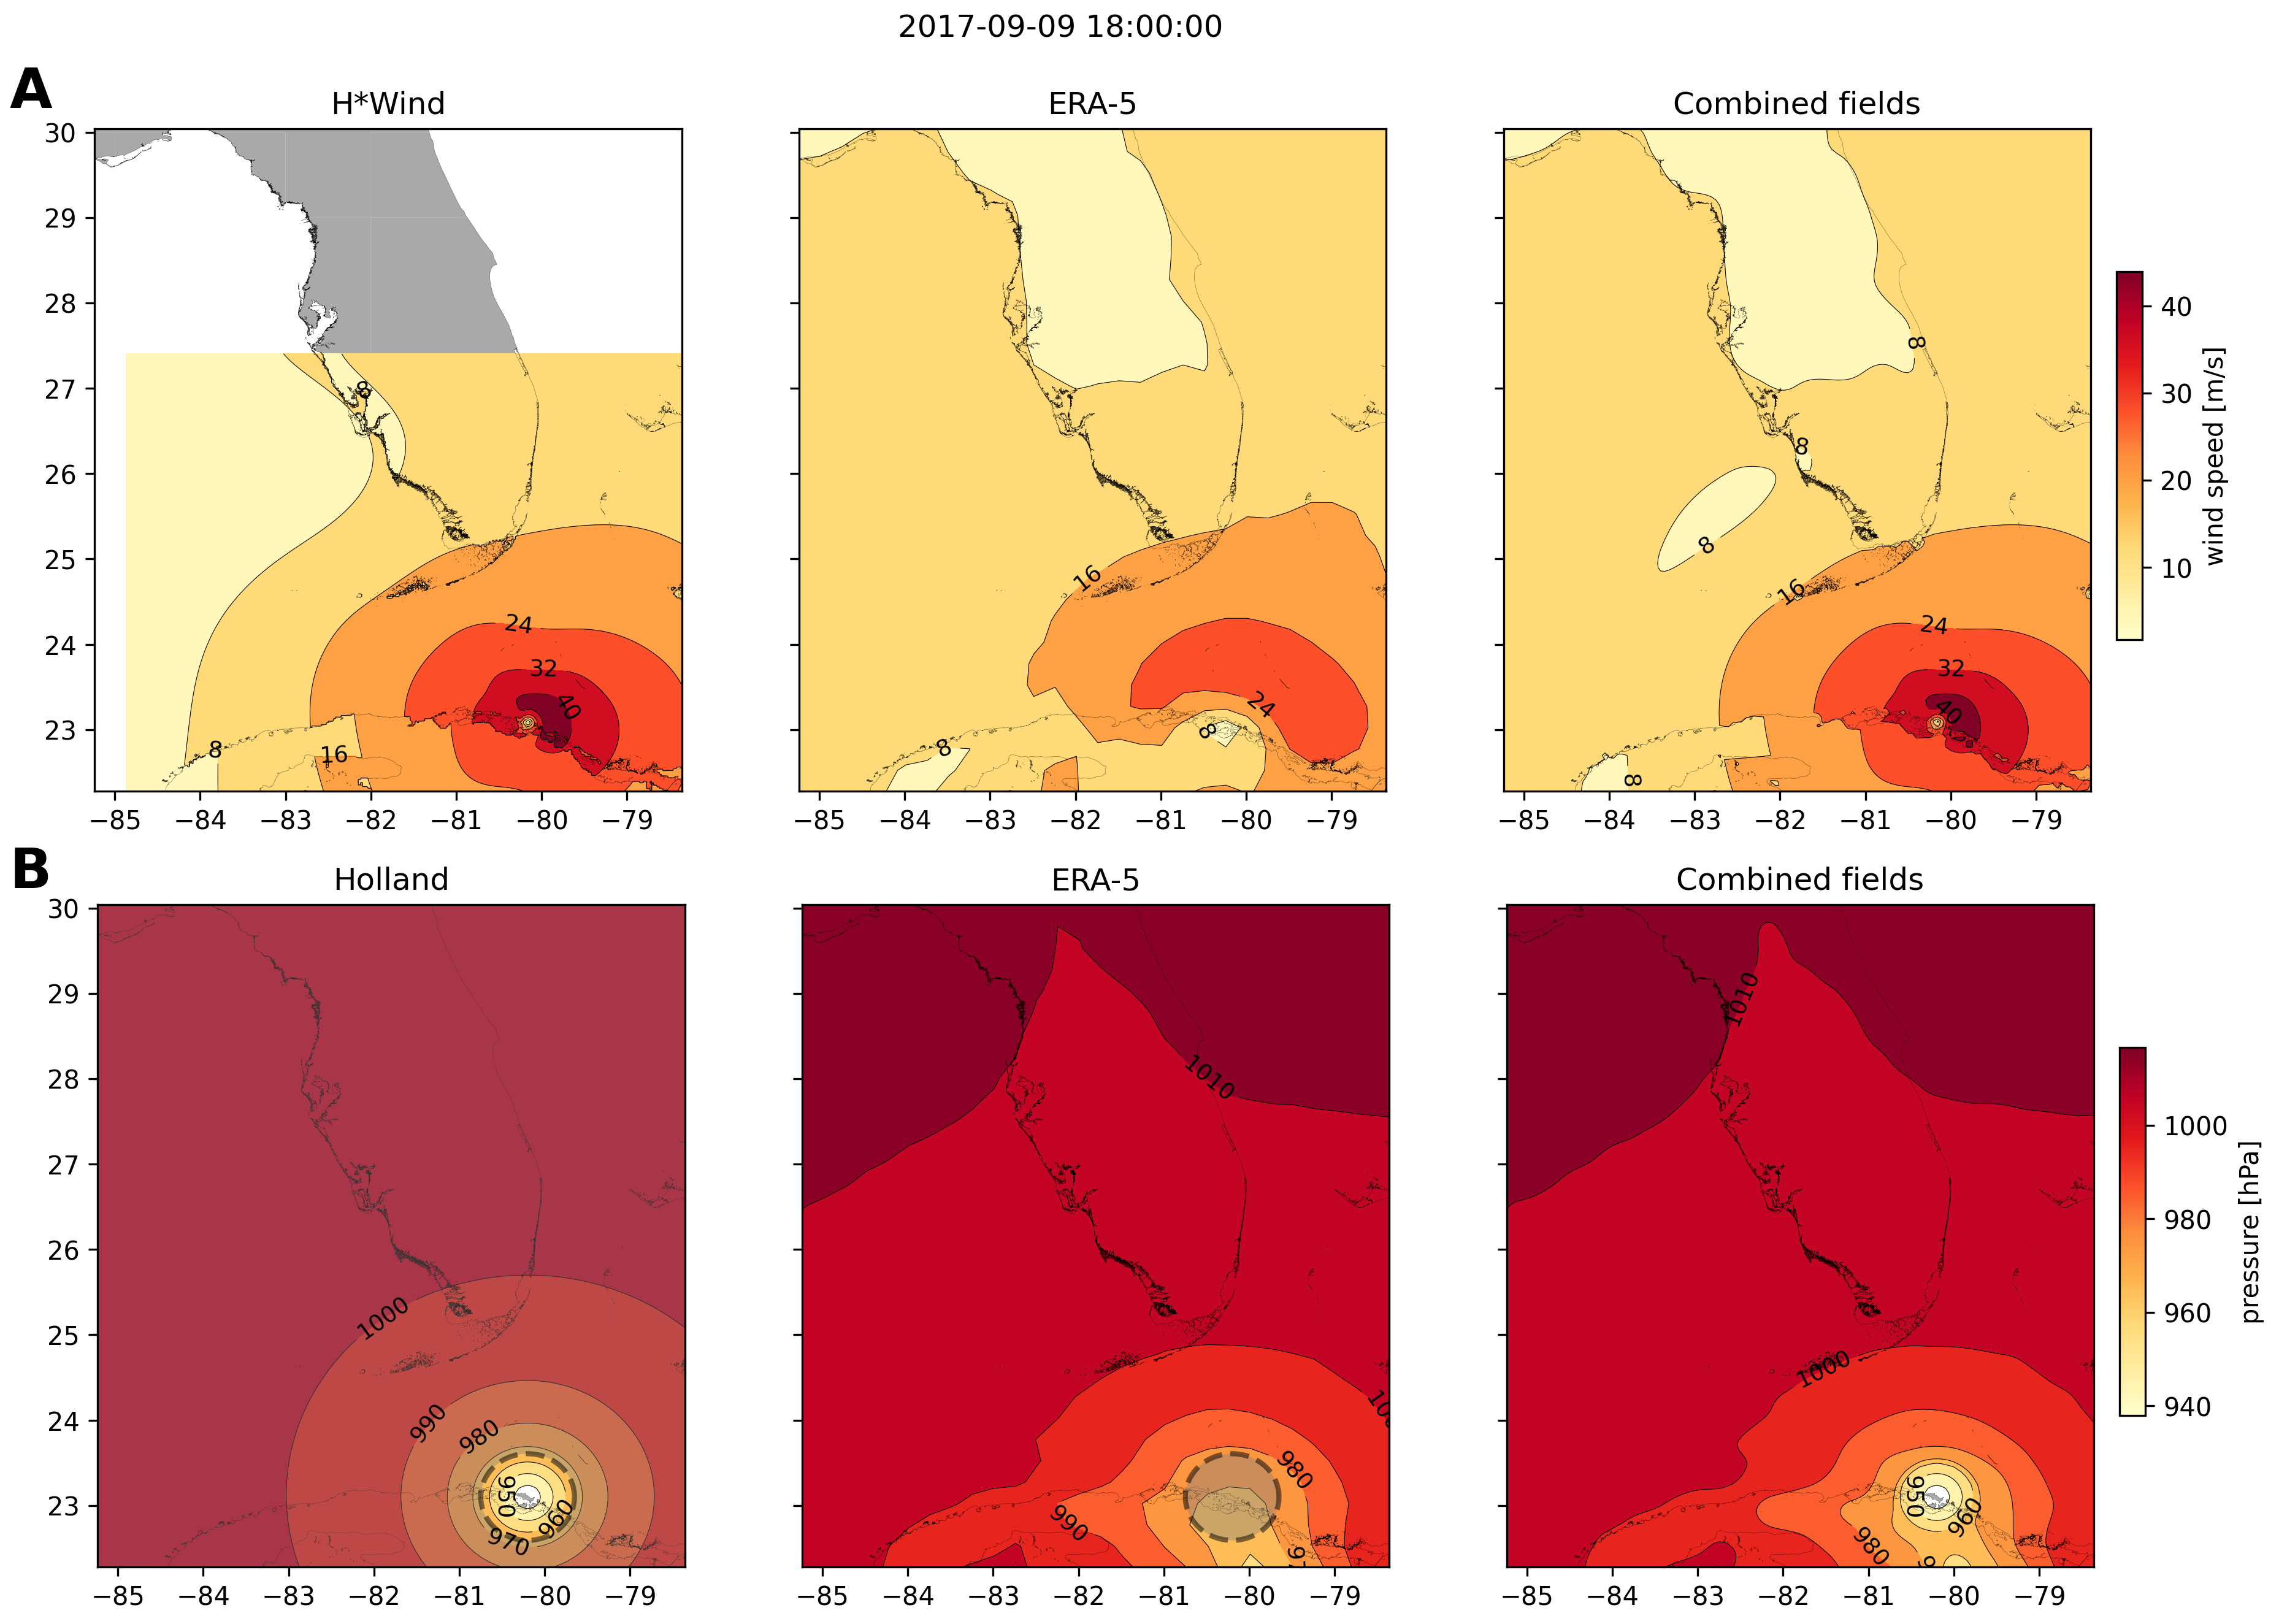
\includegraphics[width=.99\textwidth]{chapters/irma/figures/hwind+holland_vs_era.png}
    \caption{Snapshot of the hybrid wind (\textbf{A}) and pressure (\textbf{B}) profiles constructed to capture the passage of Hurricane Irma at 1800 UTC on 9 September 2017. Wind profiles were obtained by combining high resolution H*Wind with coarser ERA-5 wind fields. The pressure field was built by combining the ERA-5 pressure field with an idealized Holland pressure profile based on the track of Irma in the HURDAT 2 database. Holland field was only used within the radius of maximum wind speed (dashed grey line) of the hurricane to capture its central depression. }
    \label{fig:atm}
\end{figure}

\subsection{Hydrodynamic model}

Ocean currents generated during Hurricane Irma around South Florida were modeled using the 2D barotropic version of the unstructured-mesh Second-generation Louvain-la-neuve Ice-ocean Model\footnote{\url{https://www.slim-ocean.be}} (SLIM) \citep{lambrechts2008multi}. The model mesh covers an area similar to the model extent of \cite{dobbelaere2020coupled}, that includes the FRT but also the Florida Straits and part of the Gulf of Mexico (Figure \ref{fig:mesh}). However, this area has been slightly extended northeastward and westward in order to include the NOAA-NDBC buoys. Furthermore, to withstand potential cell drying during the hurricane, we solved the conservative shallow water equations with wetting-drying:
\begin{equation}
    \begin{split}
        \dfrac{\partial H}{\partial t} +\nabla\cdot(\UV) =& ~0~, \\
        \dfrac{\partial \UV}{\partial t}  + \nabla\cdot\left(\dfrac{\UV\UV}{H}\right) + f\mathbf{e}_z \times \UV =& ~\alpha gH\nabla(H-h) - \dfrac{1}{\rho}\nabla p_\text{atm} \\
         &+ \dfrac{1}{\rho}\text{\boldmath$\tau$}_s +\nabla\cdot(\nu\nabla\UV) \\
         &- \dfrac{C_b}{H^2}|\UV|\UV + \gamma(\UV_\text{ref}-\UV)~,
    \end{split} \label{eq:slim}
\end{equation}
where $H$ is the water column height and $\UV$ is the depth-averaged transport; $f$ is the Coriolis coefficient; $g$ is the gravitational acceleration; $h$ is the bathymetry; $\alpha$ is a coefficient indicating whether the mesh element is wet ($\alpha=1$) or dry ($\alpha=0$) \citep{le2020implicit}; $\nu$  is the Smagorinsky viscosity; $C_b$ is the bulk bottom drag coefficient; $p_\text{atm}$ is the atmospheric pressure; {\boldmath$\tau$}$_s$ is the surface stress, usually due to wind; and $\gamma$ is a relaxation coefficient towards a reference transport $\UV_\text{ref}$. As this study focuses on transport processes and not coastal flooding, wetting-drying is only applied on wet grid cells that may become dry under the influence of the hurricane. As in \cite{frys2020fine} and \cite{dobbelaere2020coupled}, SLIM currents were gradually relaxed towards the operational Navy HYbrid Coordinate Ocean Model (HYCOM) product (GOMl0.04\footnote{\url{https://www.hycom.org/data/goml0pt04}}, \cite{chassignet2007hycom}) in regions where the water depth exceeds 50 m. HYCOM's 3D currents were depth-integrated into 2D transports to be used as forcing in the model. Moreover, these transports as well as HYCOM's sea surface elevation were used as boundary condition in the model.

We adapted the parameterization of the wind-induced surface stress to storm conditions. At very high wind speeds, the white cap is blown off the crest of the waves. This phenomenon, also known as spume, has been hypothesized to generate a layer of droplets that acts as a slip layer for the winds at the ocean-atmosphere interface \citep{holthuijsen2012wind}. It causes a saturation of the wind drag coefficient for strong winds \citep{powell2003reduced,donelan2004limiting,curcic2020revised}. We take this saturation effect into account by using the wind  drag parameterization of \cite{moon2007physics}. In this parameterization, the drag coefficient $C_d$ depends on the wind speed at 10-m height $U_{10}$ according to:
\begin{equation}
    C_d = \kappa^2 \log\left(\dfrac{10}{z_0}\right)^{-2}\label{eq:drag}
\end{equation}
where $\kappa$ is the von Karman constant and $z_0$ is the roughness length expressed as: 
\begin{equation}
    z_0 =\left\{\begin{array}[]{ll}
        \dfrac{0.0185}{g}u_{\ast}^2 & \text{if }U_{10} \leq 12.5\text{ m/s}~, \\
        \lbrack 0.085(-0.56u_{\ast}^2+20.255u_{\ast} & \text{if }U_{10} > 12.5\text{ m/s}~, \\
        \quad +2.458) - 0.58\rbrack\times 10^{-3} 
    \end{array}\right.
\end{equation}
with $u_\ast$ the friction velocity. The relation between $U_{10}$ and $u_{\ast}$ is given by:
\begin{equation}
    U_{10}=-0.56u_{\ast}^2+20.255u_{\ast}+2.458~.
\end{equation}

The mesh resolution depends on the distance to the coastlines and reefs following the approach of \cite{dobbelaere2020coupled}. The mesh is then further refined according to bathymetry value and gradient, as suggested in the SWAN user-guide\footnote{\url{http://swanmodel.sourceforge.net/unswan/unswan.htm}}. Such an approach improves the model efficiency as the mesh resolution is only increased where required by the currents and waves dynamics. The mesh was generated with the seamsh\footnote{\url{https://pypi.org/project/seamsh/}} Python library, which is based on the the open-source mesh generator GMSH \citep{geuzaine2009gmsh}. It is composed of approximately 7.7 $\times$ 10$^5$ elements. The coarsest elements, far away from the FRT, have a characteristic length of about 5 km whereas the finest elements have a characteristic length of about 100 m along the coastlines and over the reefs (Fig \ref{fig:mesh}).

\subsection{Wave model}
Waves were modeled using the parallel unstructured-mesh version of the Simulating WAves Nearshore (SWAN) model \citep{booij1999third}, one of the most popular wave models for coastal areas and inland waters. It solves the action balance equation \citep{mei1989applied}:
\begin{equation}
    \dfrac{\partial N}{\partial t} + \nabla_\mathbf{x}\cdot[(\mathbf{c}_g+\mathbf{u})N] + \dfrac{\partial }{\partial \theta}[c_\theta N] + \dfrac{\partial}{\partial \sigma}[c_\sigma N] = \dfrac{S_{in}+S_{ds}+S_{nl}}{\sigma}~, \label{eq:swan}
\end{equation}
where $N=E/\sigma$ is the wave action density and $E$ is the wave energy spectrum; $\theta$ is the wave propagation direction; $\sigma$ is the intrinsic wave frequency; $\mathbf{c}_g$ is the wave group velocity, $\mathbf{u}=\mathbf{U}/H$ is SLIM depth-averaged current velocity; $c_\theta$ and $c_\sigma$ are the propagation velocities in spectral space due to refraction and shifting in frequency due to variations in depth and currents; and $S_{in}$, $S_{ds}$, and $S_{nl}$ respectively represent wave growth by wind, wave decay and nonlinear transfers of wave energy through four and three-wave interactions, \ie~quadruplets and triplets. The wave spectra were discretized with 48 direction bins and 50 frequency bins logarithmically distributed from 0.03 to 2 Hz. Exponential wind growth was parameterized using the formulation of \cite{janssen1991quasi}, while dissipations by whitecapping and bottom dissipation followed the formulations of \cite{komen1984existence} and \cite{madsen1989spectral}, respectively.

Coefficients for exponential wind growth and whitecapping parameterizations were based on the results of \cite{siadatmousavi2011evaluation}, and significantly differ from SWAN's default settings. By default, SWAN implements the wind input formulation of \cite{komen1984existence} and the steepness-dependent coefficient governing dissipation by whitecapping is a linear function of the wavenumber. In this study, this steepness-dependent coefficient is a quadratic function of the wavenumber, as it showed better predictions of the significant wave height in the study of \cite{siadatmousavi2011evaluation}. The choice of these formulations was motivated by the appearance of numerical instabilities in the region of the Gulf Stream when using SWAN's default parameter values. Finally, ERA-5 wave spectra was used as boundary condition for SWAN. Wave spectra is obtained from the ocean wave model WAM and is given on a $1^\circ \times 1^\circ$ grid with 24 directions and 36 frequencies.

Surface waves induce a net drift in the direction of the wave propagation, known as the Stokes drift \citep{van2018stokes,stokes1880theory}. This net drift has a significant impact on sediment transport in nearshore regions \citep{hoefel2003wave}, on the formation of Langmuir cells \citep{langmuir1938surface, craik1976rational} as well as on the transport of heat, salt or pollutants such as oil or micro-plastic in the upper ocean layer \citep{mcwilliams2000vertical,rohrs2012observation,drivdal2014wave}. To correctly model the Stokes drift profile in mixed wind-driven sea and swell conditions, the full two-dimensional wave spectrum must be represented by a spectral wave model within a wave-current coupling \citep{van2018stokes}. We therefore used SWAN modeled spectra to compute the Stokes drift as follows:
\begin{equation}
    \mathbf{u}_{s} = \int_0^{2\pi}\int_0^{+\infty} \dfrac{\sigma^3}{h\tanh(2kh)}E(\sigma,\theta)(\cos\theta, \sin\theta)d\sigma d\theta~, \label{eq:stokes}
\end{equation}
where $k$ is the norm of the wave vector; $h$ is the water depth; and $E(\sigma,\theta)$ is the wave energy density. The computed Stokes drift velocity is then added to SLIM depth-averaged current velocity to transport drifting particles in the experiments described in section \ref{sec:traj}.

\subsection{Coupled model}

SLIM and SWAN are coupled so that they run on the same computational core and the same unstructured mesh. SLIM is run first and passes the wind velocity ($\mathbf{U}_{10}$), water level ($\eta=H-h$) and depth-averaged current ($\mathbf{u}=\mathbf{U}/H$) fields to SWAN, as well as a roughness length ($z_0$) for the bottom dissipation formulation of \cite{madsen1989spectral}. This roughness length is computed from SLIM's bulk drag coefficient $C_b$ following the approach of \cite{dietrich2011hurricane} so that both models have consistent bottom dissipation parameterizations. SWAN then uses these quantities to compute the wave radiation stress gradient, that is then passed to SLIM as the force exerted by waves on currents {\boldmath$\tau$}$_\text{wave}$ (Fig. \ref{fig:coupling}). SLIM then uses this quantity to update the value of the surface stress {\boldmath$\tau$}$_s$ in Eq. (\ref{eq:slim}), that now becomes the sum of wind and wave-induced stresses $\text{\boldmath$\tau$}_s = \text{\boldmath$\tau$}_\text{wind}+\text{\boldmath$\tau$}_\text{wave}$. Here, the momentum flux from the atmosphere to the ocean is taken as the usual full wind stress {\boldmath$\tau$}$_\text{wind}$. Doing so, we neglect the momentum advected away from the storm by the waves, leading to a 10-15\% overestimation of the momentum flux in hurricane winds \citep{curcic2015explicit}.

We followed the approach of \cite{dietrich2012performance} by characterizing the wave-induced forces on currents using the radiation-stress (RS) gradient formalism, which has been successfully applied in both 2D and 3D coupled wave-current models under storm conditions \citep{hope2013hindcast, sebastian2014characterizing, brown2013depth}. \modif{In this formalism, wave-averaged effects are characterized by the divergence of a stress tensor representing the flux of momentum to currents due to surface gravity waves \citep{longuet1964radiation,lane2007wave,kumar2012implementation}}. An alternative formalism is the vortex-force (VF) representation \citep{mcwilliams2004asymptotic}, that provides a clearer decomposition of the wave effect \citep{lane2007wave}. \modif{Here, wave impact on current is represented by the combination of the gradient of a Bernoulli head representing adjustments to the pressure in incompressible fluids, and the interaction of the Stokes drift with the vorticity of the flow, \textit{i.e.} the vortex force \citep{lane2007wave}}. Although both approaches were adopted by coastal modeling communities, there is an ongoing scientific debate over the correctness and applicability of the two concepts \citep{ardhuin2008comments, mellor2013waves, mellor2015combined, ardhuin2017comments}. \cite{xia2020implementation} recently implemented the two formalisms in a 3D unstructured-grid model and compared them in three typical coastal systems, showing that the 3D RS algorithm could generate unrealistic offshore currents near shorelines. Despite these shortcomings, the 3D RS method reproduced most wave-induced currents and the 2D RS formalism remains a well-validated modeling approach. Furthermore, \cite{mellor2013waves} showed that the RS approach was valid when $[\frac{\partial H}{\partial\mathbf{x}}/\sinh(kh)]^2$ is smaller or of the same order as $(ka)^2$, where $a$ is the wave amplitude. We evaluated these quantities and verified that the validity criterion was met in our model domain. Additionally, since the VF and RS approached are formally equivalent \citep{lane2007wave}, we selected the 2D RS formalism, as it has the advantage of summarizing the impact of waves on the currents in a single additional stress term in the hydrodynamic model equations.

SLIM's governing equations are integrated using an implicit time integration scheme while SWAN is unconditionally stable \citep{dietrich2012performance}, allowing both models to be run with relatively large time steps. In this study, the stationary version of SWAN was used, \ie~the first term of Eq. (\ref{eq:swan}) was set to zero. This resulted in reduced scaling and convergence rates than with the nonstationary version of SWAN but increased the model stability. The wave spectra at each node of the mesh was saved at the end of each iteration to serve as initial conditions for the next one. Both models were run sequentially using a time step of 600 s, so that each computational core was alternatively running either SLIM or SWAN. As in the coupling between SWAN and the ADvanced CIRCulation model (ADCIRC) \citep{dietrich2012performance}, both models use the same local sub-mesh, allowing for a one-to-one correspondence between the geographic locations of the mesh vertices. No interpolation is therefore needed when passing the discretised variables from one model to the other, which allows an efficient inter-model communication. However, as SLIM is based on  a discontinuous Galerkin finite element method, an additional conversion step to a continuous framework was required to transfer SLIM nodal quantities to SWAN. The coupling increases the computation time by 3\% as compared to the sum of the uncoupled SLIM and SWAN simulations wall-clock times for the same number of CPUs and the same simulation period.
%The coupling increased the computation time by 400\% and 25\% respectively compared to uncoupled SLIM and SWAN model runs with the same number of CPUs over the same simulated period.

% Wall time simulations
%   - slim     : 00:56:56 ->  3416 s
%   - swan     : 03:56:57 -> 14217 s
%   - coupled  : 05:02:51 -> 18171 s
% => overshoot of 538 sec -> increase computation time by 3%

\begin{figure}
    \centering
    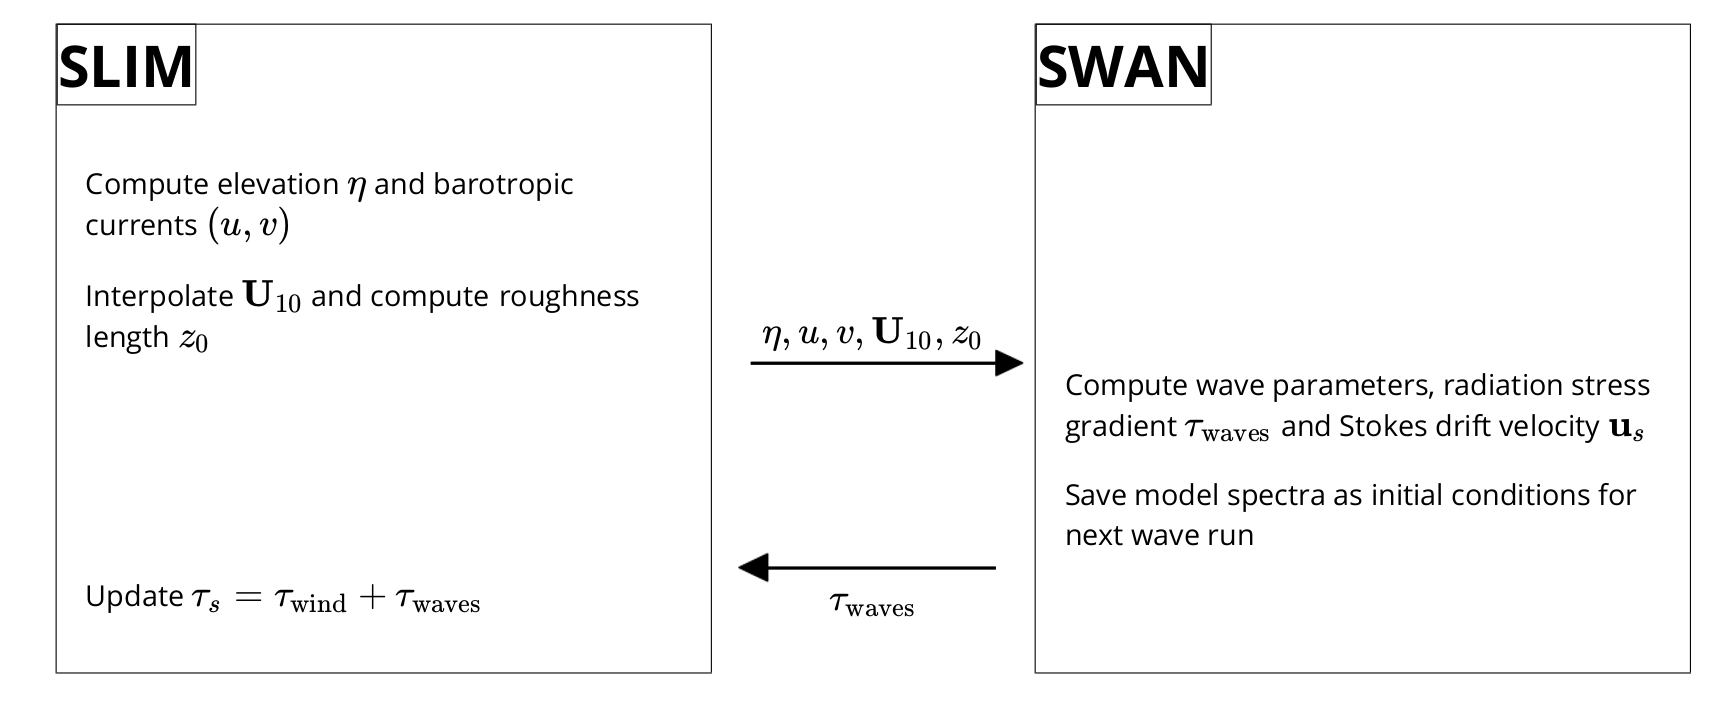
\includegraphics[width=.99\textwidth]{chapters/irma/figures/coupling_v2.png}
    \caption{Schematic illustration of the coupled SLIM+SWAN model. \modif{Both models run on the same computational cores and mesh. SLIM is run first and passes the wind velocity $U_{10}$, water level $\eta$, depth-averaged current $u$ and bottom roughness length $z_0$ to SWAN. SWAN then uses these quantities to compute the wave radiation stress gradient $\text{\boldmath$\tau$}_\text{wave}$, that is then passed
    to SLIM as the force exerted by waves on currents. SLIM then uses this quantity to update the value of the surface stress $\text{\boldmath$\tau$}_s$, computed as the combination of wind and wave stresses $\text{\boldmath$\tau$}_\text{wind} + \text{\boldmath$\tau$}_\text{wave}$}}
    \label{fig:coupling}
\end{figure}

\subsection{Quantifying the effect of wave-current interactions on transport}\label{sec:traj}

To quantify the impact of wave-current interactions on transport processes, we compared the trajectories of passive particles advected by the uncoupled SLIM and coupled SLIM+SWAN currents during the passage of Irma in the Lower Keys. Furthermore, the depth-averaged Stokes drift was computed using the wave spectra of the coupled model SLIM+SWAN run as well as those of an uncoupled SWAN run. Particles were released on the inner and outer shelves at the points highlighted by red and blue dots in Fig. \ref{fig:init} on Sept. 7 at 0000 UTC and then tracked until Sept. 15. These initial particle positions were found using backtracking methods \citep{spivakovskaya2005simulation} \modif{to obtain a probabilistic picture of the release positions from which particles would intersect the path of Irma during its passage through the Florida Keys}. We first defined two 25 km$^\text{2}$ circular regions on the trajectory of the hurricane (see red and blue circles in Fig. \ref{fig:init}). Particles within these two regions were then tracked backward in time using uncoupled SLIM currents from the exact time of the passage of the hurricane until Sept. 7 at 0000 UTC. Their positions at the end of the backward simulation (see red and blue particle clouds in Fig. \ref{fig:init}) corresponds to the initial condition of the forward transport simulations described below. We then compared the trajectories of particles originating from these regions and advected forward in time by different sets of currents: (i) uncoupled SLIM currents alone; (ii) coupled SLIM+SWAN currents; (iii) SLIM currents with the addition of the depth-averaged Stokes drift computed with the coupled wave-current model (Stokes-C); (iv) SLIM+SWAN currents with Stokes-C; and (v) SLIM currents with the depth-averaged Stokes drift computed with the uncoupled wave model (Stokes-U). The different combinations of Eulerian currents and Stokes drifts used to model the transport of passive drifters in the Lower Keys during the passage of Irma are summarized in Table \ref{tab:summary}. Particle trajectories are compared by computing the distances between the centers of mass of the particle clouds through time.

\begin{figure}
    \centering
    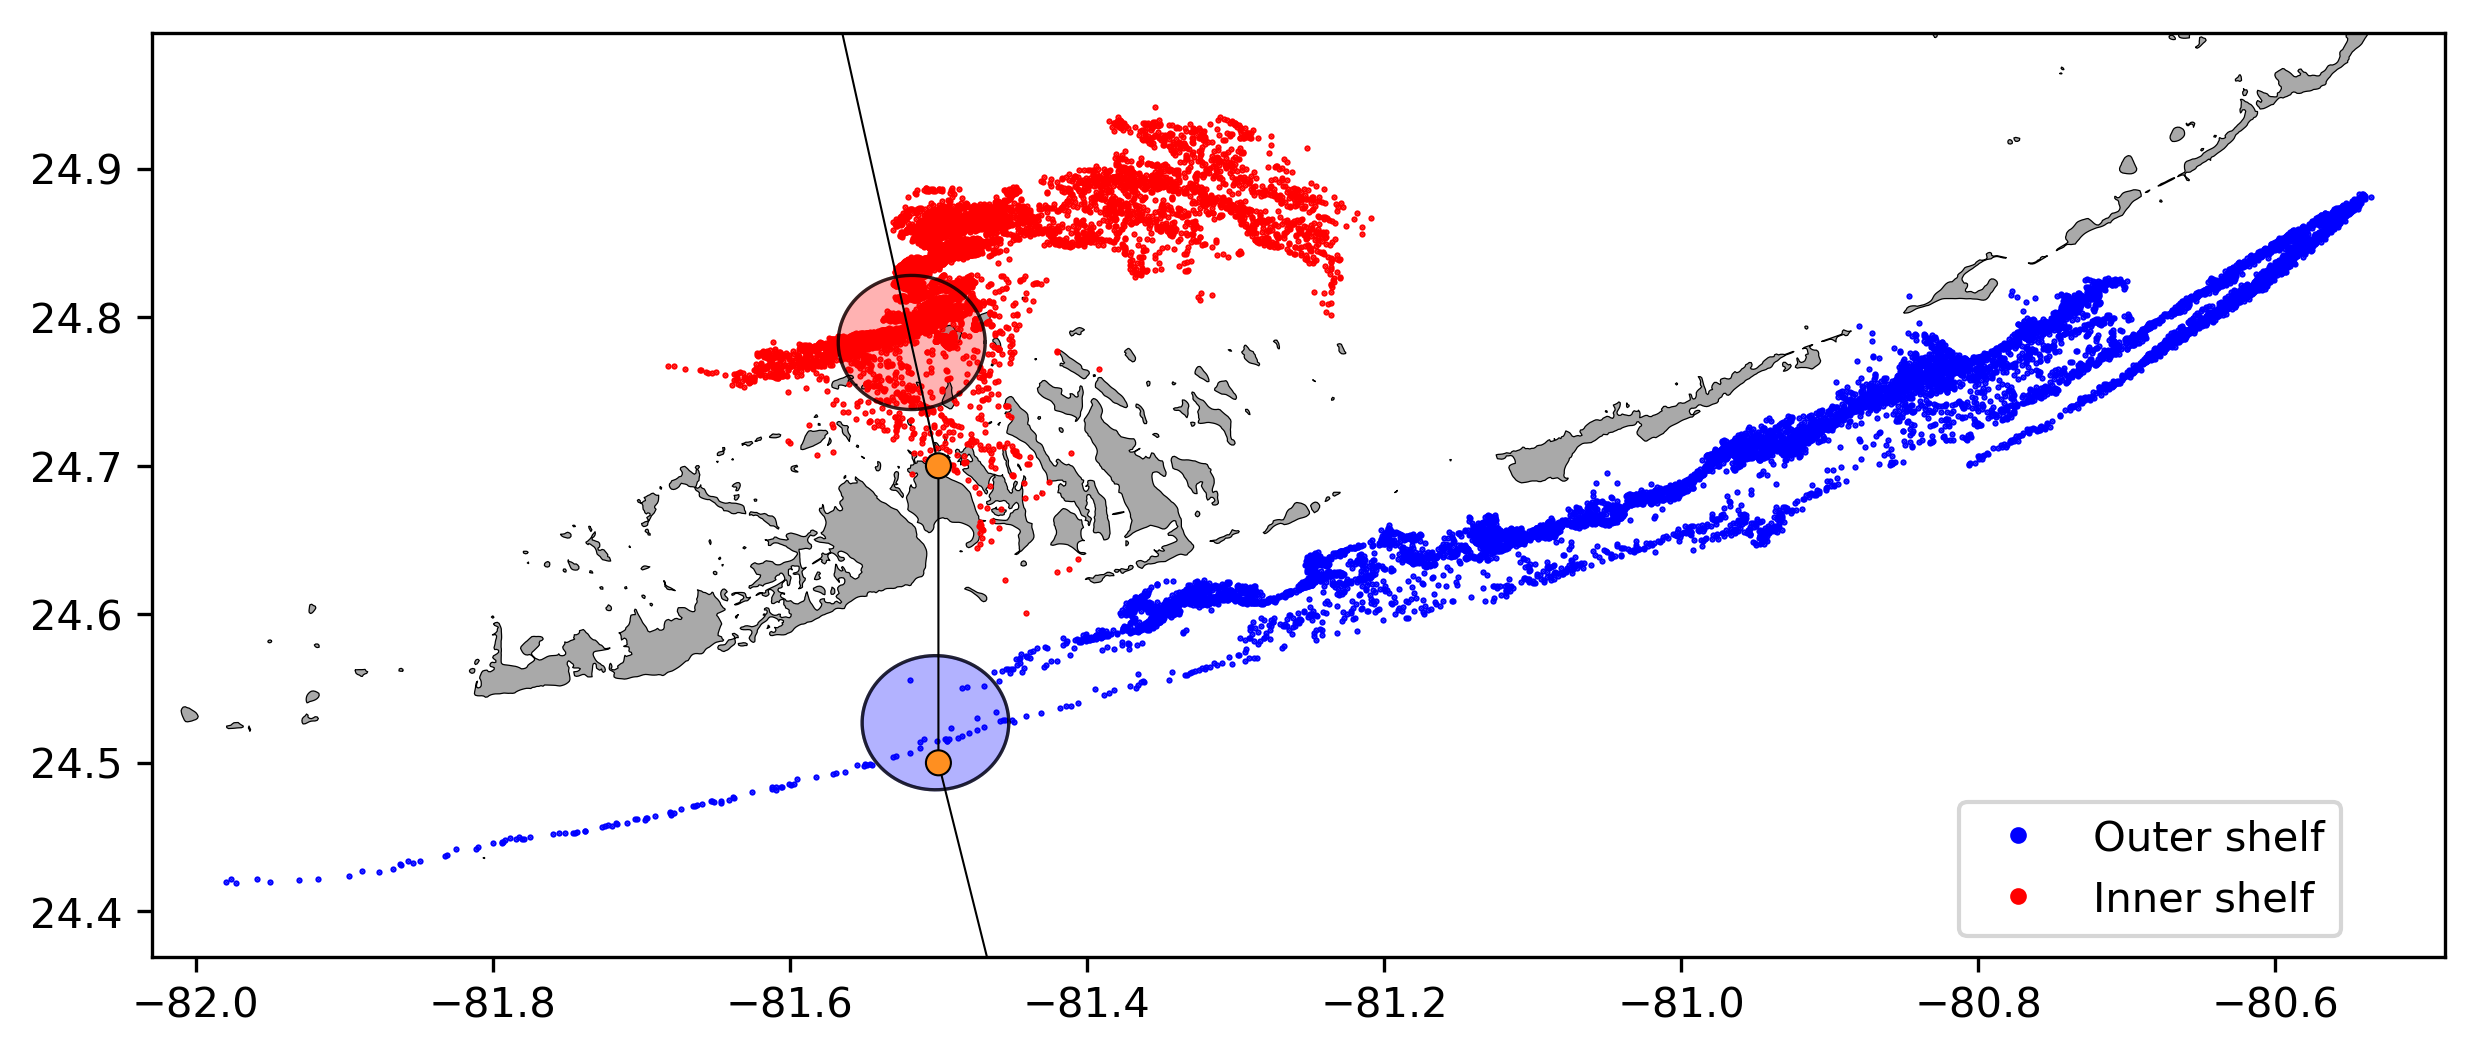
\includegraphics[width=.95\textwidth]{chapters/irma/figures/figure_initial_positions.png}
    \caption{Release regions of the passive particles on the inner and outer shelves on Sept 7 at 0000 UTC (red and blue clouds) obtained by backtracking particles released in the red and blue circular areas during the passage of Irma. \modif{These clouds give a probabilistic picture of the positions from which particles should have been released to intersect the path of the center of the hurricane}}
    \label{fig:init}
\end{figure}

\begin{table}
    \centering
%    \begin{tabular}{|p{4.5cm}|p{8cm}|}
%        \hline
%        \textbf{Experiment name} & \textbf{Model description} \\ \hline
%        SLIM               & Eulerian currents from the uncoupled SLIM simulation \\ \hline
%        SLIM+SWAN          & Eulerian currents impacted by the RS gradient from the coupled SLIM+SWAN simulation \\ \hline
%        SLIM+Stokes-U      & Eulerian currents from the uncoupled SLIM run with the Stokes drift from the uncoupled SWAN simulation \\ \hline
%        SLIM+Stokes-C      & Eulerian currents from the uncoupled SLIM run with the Stokes drift from the coupled SLIM+SWAN simulation \\ \hline
%        SLIM+SWAN+Stokes-C & Eulerian currents impacted by the RS gradient and the Stokes drift from the coupled SLIM+SWAN simulation \\ \hline
%    \end{tabular}
    \begin{tabular}{|p{3.5cm}|p{3.25cm}|p{3.2cm}|}
        \hline
        \textbf{Experiment name} & \textbf{Eulerian currents from} &  \textbf{Stokes drift from}\\ \hline
        SLIM               & uncoupled SLIM simulation & None \\ \hline
        SLIM+SWAN          & coupled SLIM+SWAN simulation (impacted by RS gradient) & None \\ \hline
        SLIM+Stokes-U      & uncoupled SLIM simulation & uncoupled SWAN simulation \\ \hline
        SLIM+Stokes-C      & uncoupled SLIM simulation & coupled SLIM+SWAN simulation \\ \hline
        SLIM+SWAN+Stokes-C & coupled SLIM+SWAN simulation (impacted by RS gradient) & coupled SLIM+SWAN simulation \\ \hline
    \end{tabular}
    \caption{Summary of the different combinations of Eulerian currents and Stokes drifts used to model the transport of passive drifters on the passage of Hurricane Irma in the Lower Keys}
    \label{tab:summary}
\end{table}

%%%%%%%%%%%%%%%%%%%
% --- RESULTS --- %
%%%%%%%%%%%%%%%%%%%
\section{Results}

We first validated the reconstructed atmospheric fields of Hurricane Irma as well as the outputs of our coupled wave-current model against field measurements. We then used the validated model outputs to simulate the transport of passive particles in the Lower Keys during the passage of Hurricane Irma. These particles were advected by the sets of currents described in Table \ref{tab:summary} and their trajectories were compared to evaluate the impact of the wave-current interactions and the Stokes drift on the transport processes during the passage of Irma.

\subsection{Model validation}

H*Wind winds and hybrid pressure field agree well with station measurements at Vaca Key station (Fig. \ref{fig:forcings}). The hybrid pressure field shows a better agreement with observations than ERA-5 pressure as it successfully reproduces the storm depression. ERA-5 fields, on the other hand, fail to reproduce the low pressure at the core of the hurricane due to their coarser grid, leading to an overestimation of 8 mbar of the storm depression. Both H*Wind and ERA-5 agree well with observed wind speeds although both data sets tend to slightly overestimate the width and intensity of the wind peak. However, H*Wind profiles better reproduce the timing of the observed peak, as ERA-5 winds tend to anticipate it. H*wind also exhibits a slightly narrower peak in wind speed, which better agrees with observations.

\begin{figure}
    \centering
    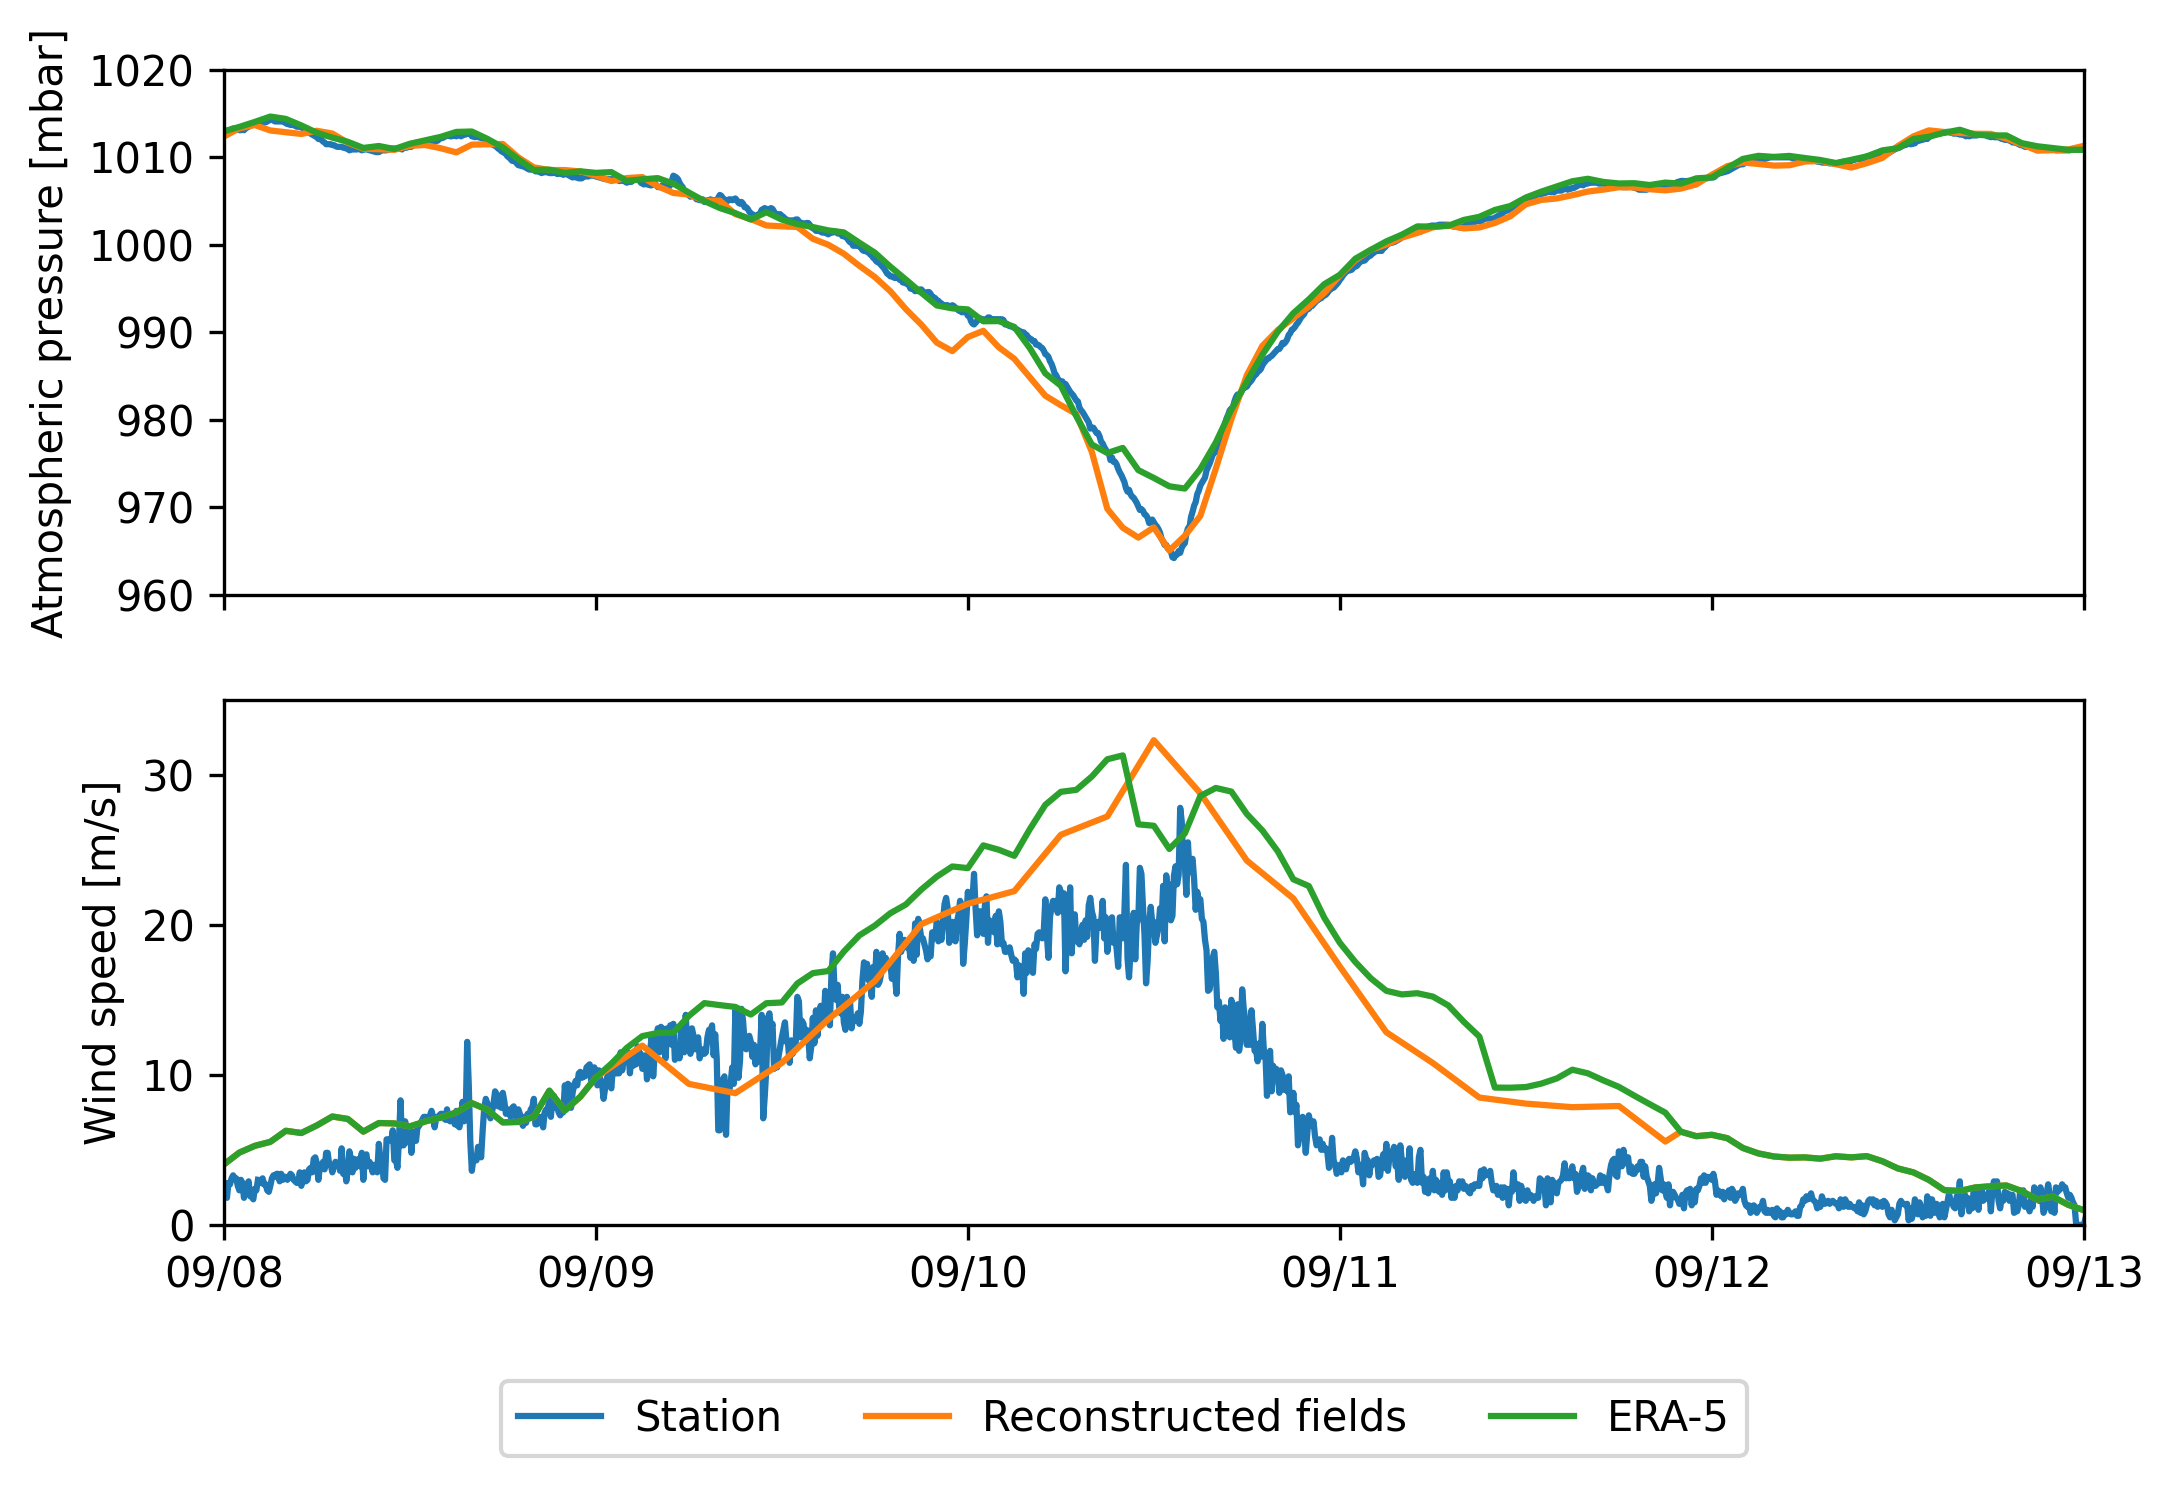
\includegraphics[width=.95\textwidth]{chapters/irma/figures/validation_met_2.png}
    \caption{Comparison of reconstructed atmospheric pressure (top) and wind speed (bottom) with field measurements and coarser ECMWF ERA-5 profiles at Vaca Key station. The generated hybrid atmospheric forcings better reproduce the observed storm depression while H*wind winds better reproduce the measured peak in wind speed.}
    \label{fig:forcings}
\end{figure}

Hydrodynamic outputs of the coupled wave-current model agree well with tide gauge (Fig. \ref{fig:sse}) and ADCP measurements (Fig. \ref{fig:uv}). The coupled model reproduces well the timing of the positive and negative storm surges at all tide gauge locations. The amplitude of the positive surges are especially well captured at Naples and Vaca Key, with errors of 2 and 6 centimeters respectively. However, the model underestimates the positive surges at Virginia Key and Key West by 24\% and 15\% at the peak respectively. The amplitude of the negative surge at Naples is also underestimated by about 16\% at the peak. Nonetheless, on average, the absolute error between the model and observations does not exceed 10 cm (Table \ref{tab:stat}). Modeled 2D currents were validated against depth-averaged ADCP measurements at mooring stations C10, C12 and C13 (Fig. \ref{fig:uv}). As in \cite{liu2020impacts}, we performed the vector correlation analysis of \cite{kundu1976ekman} to compare modeled and observed current velocity vectors. Correlation coefficients ($\rho$) between simulated and observed depth-averaged currents are 0.87, 0.84 and 0.81 at stations C10, C12 and C13, respectively. The average veering angles are below 12$^\circ$, as in \citep{liu2020impacts}. Furthermore, the positive bias in Table \ref{tab:stat} indicates that our model tends to underestimate the southward component of the currents at the different stations. As expected from a depth-averaged model, the best fit with observations is obtained at the shallowest mooring C10, located on the 25 m isobath. 

\begin{figure}
    \centering
    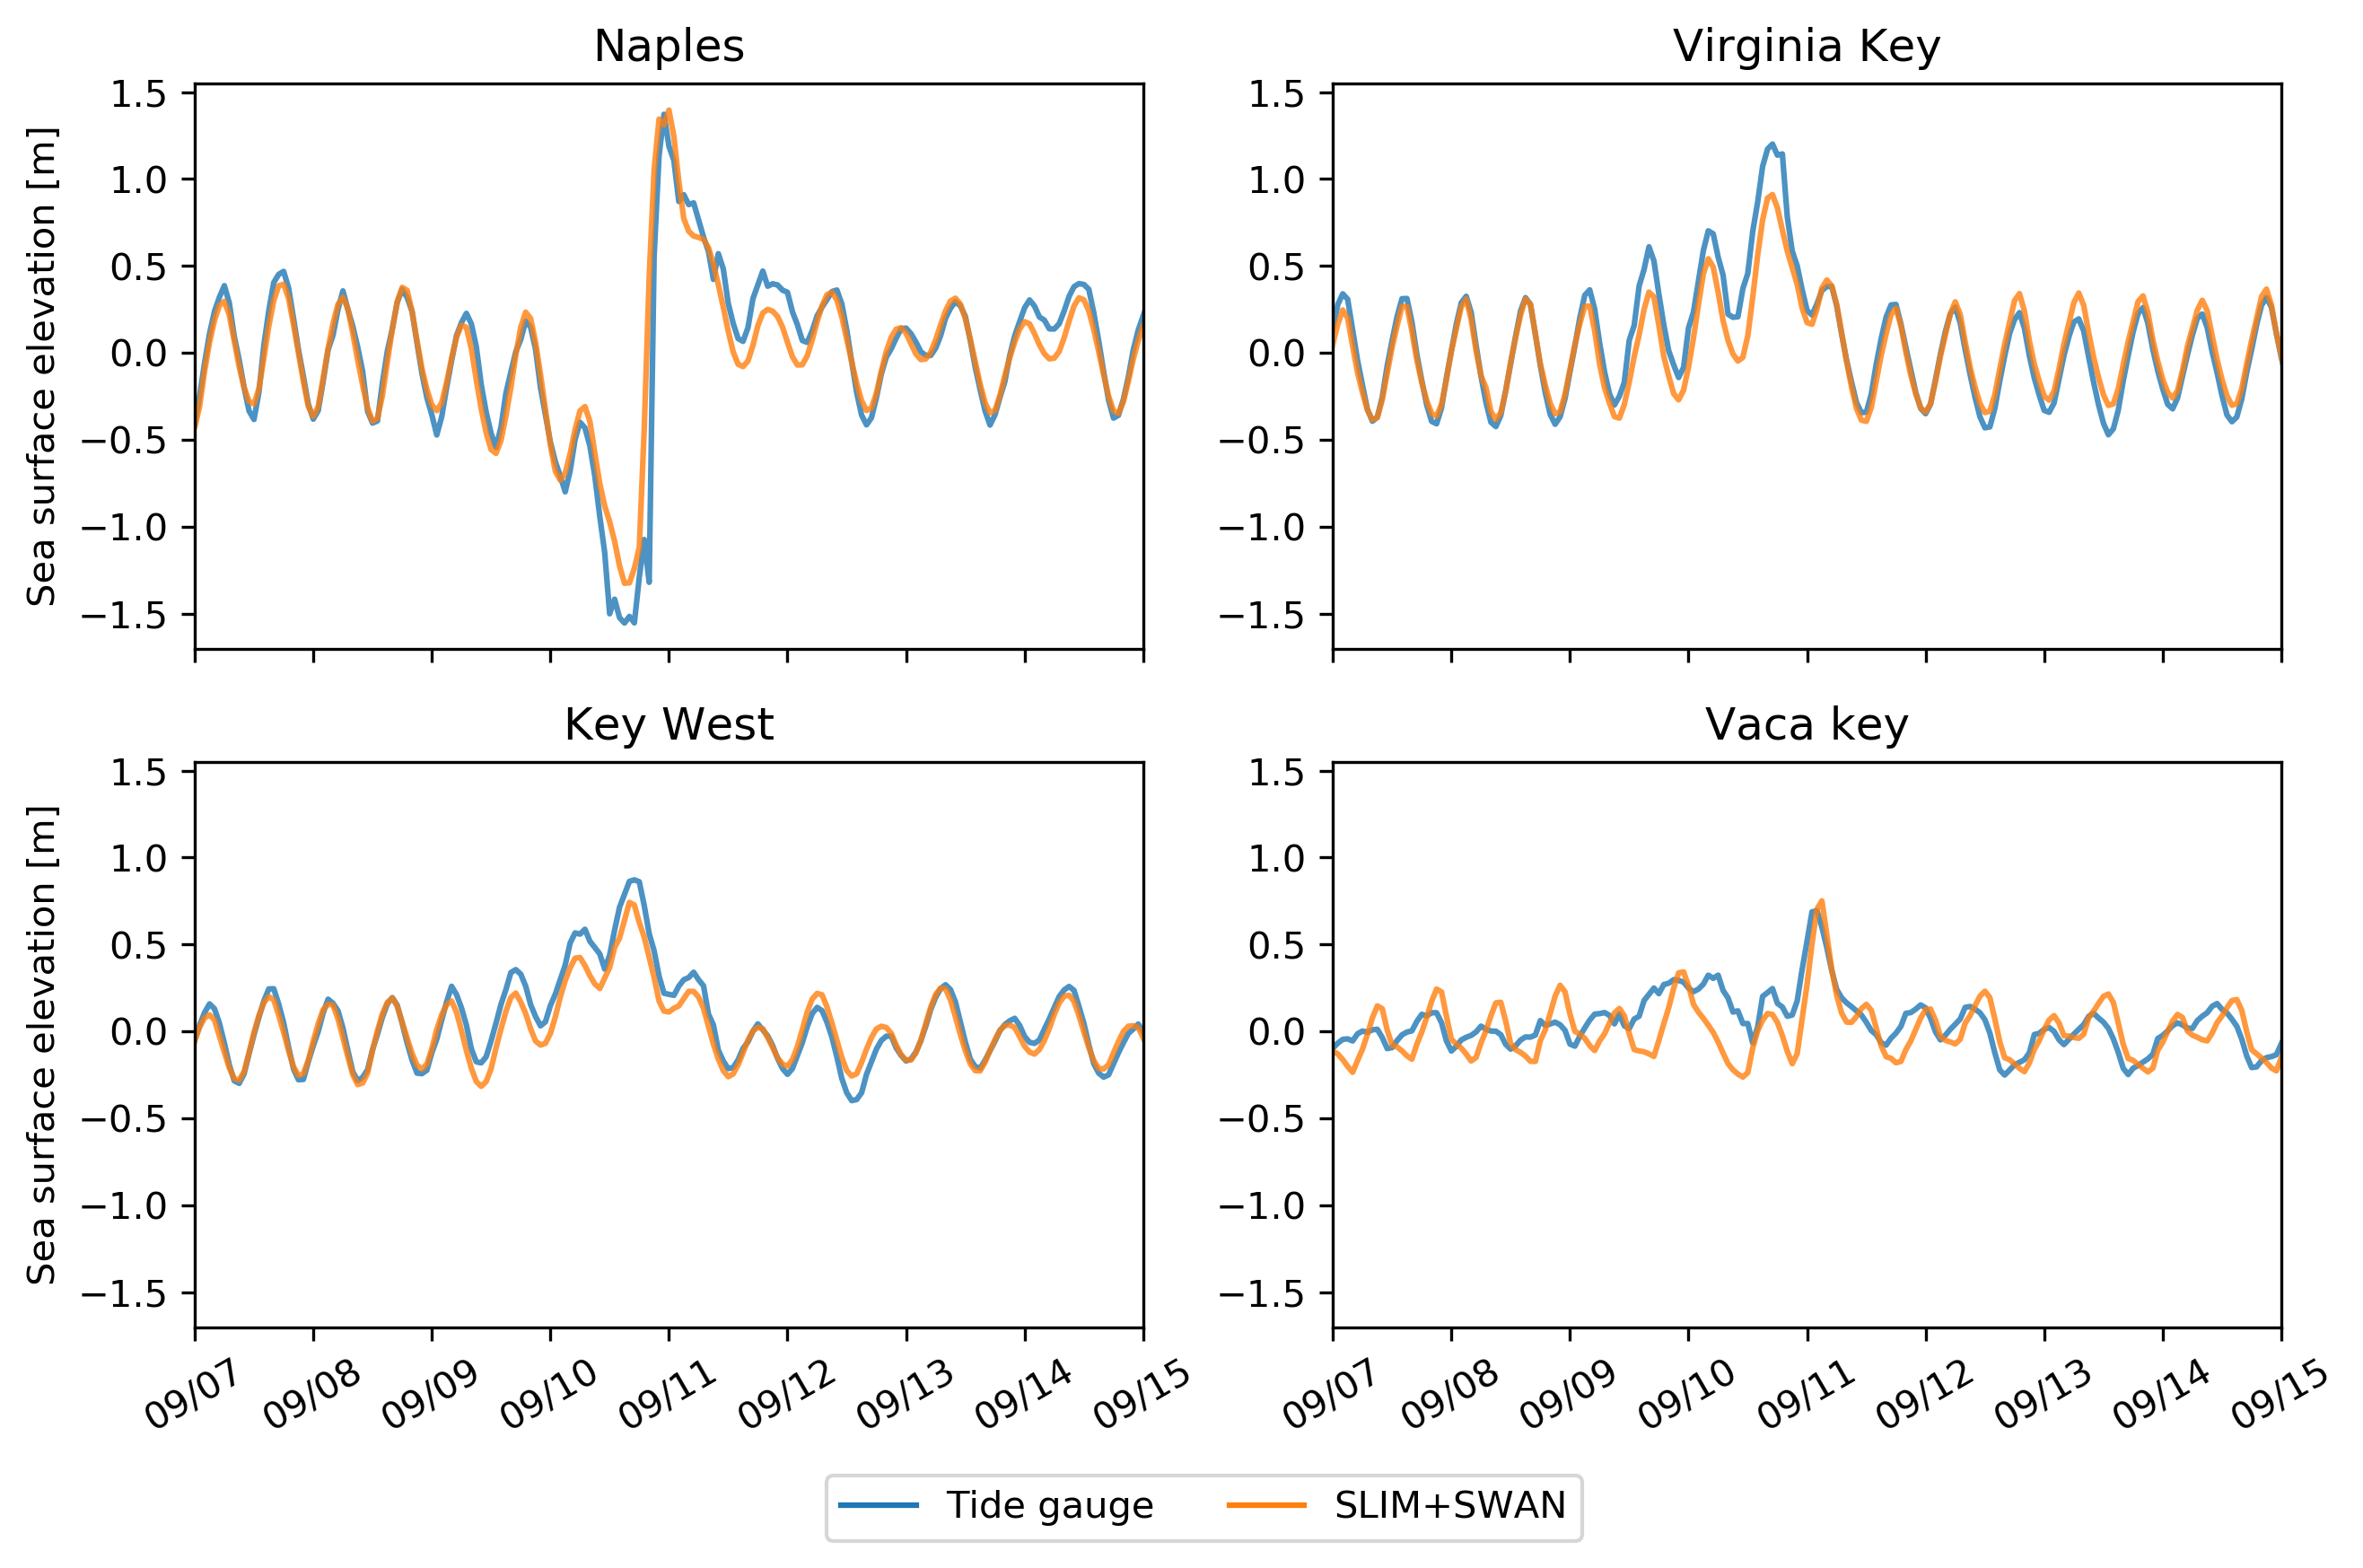
\includegraphics[width=\textwidth]{chapters/irma/figures/validation_eta.png}
    \caption{Comparison of modeled sea surface elevation at the 4 tide gauges shown in Fig. \ref{fig:mesh}B. The timing and amplitude of the storm surges are well reproduced by the model}
    \label{fig:sse}
\end{figure}
\begin{figure}
    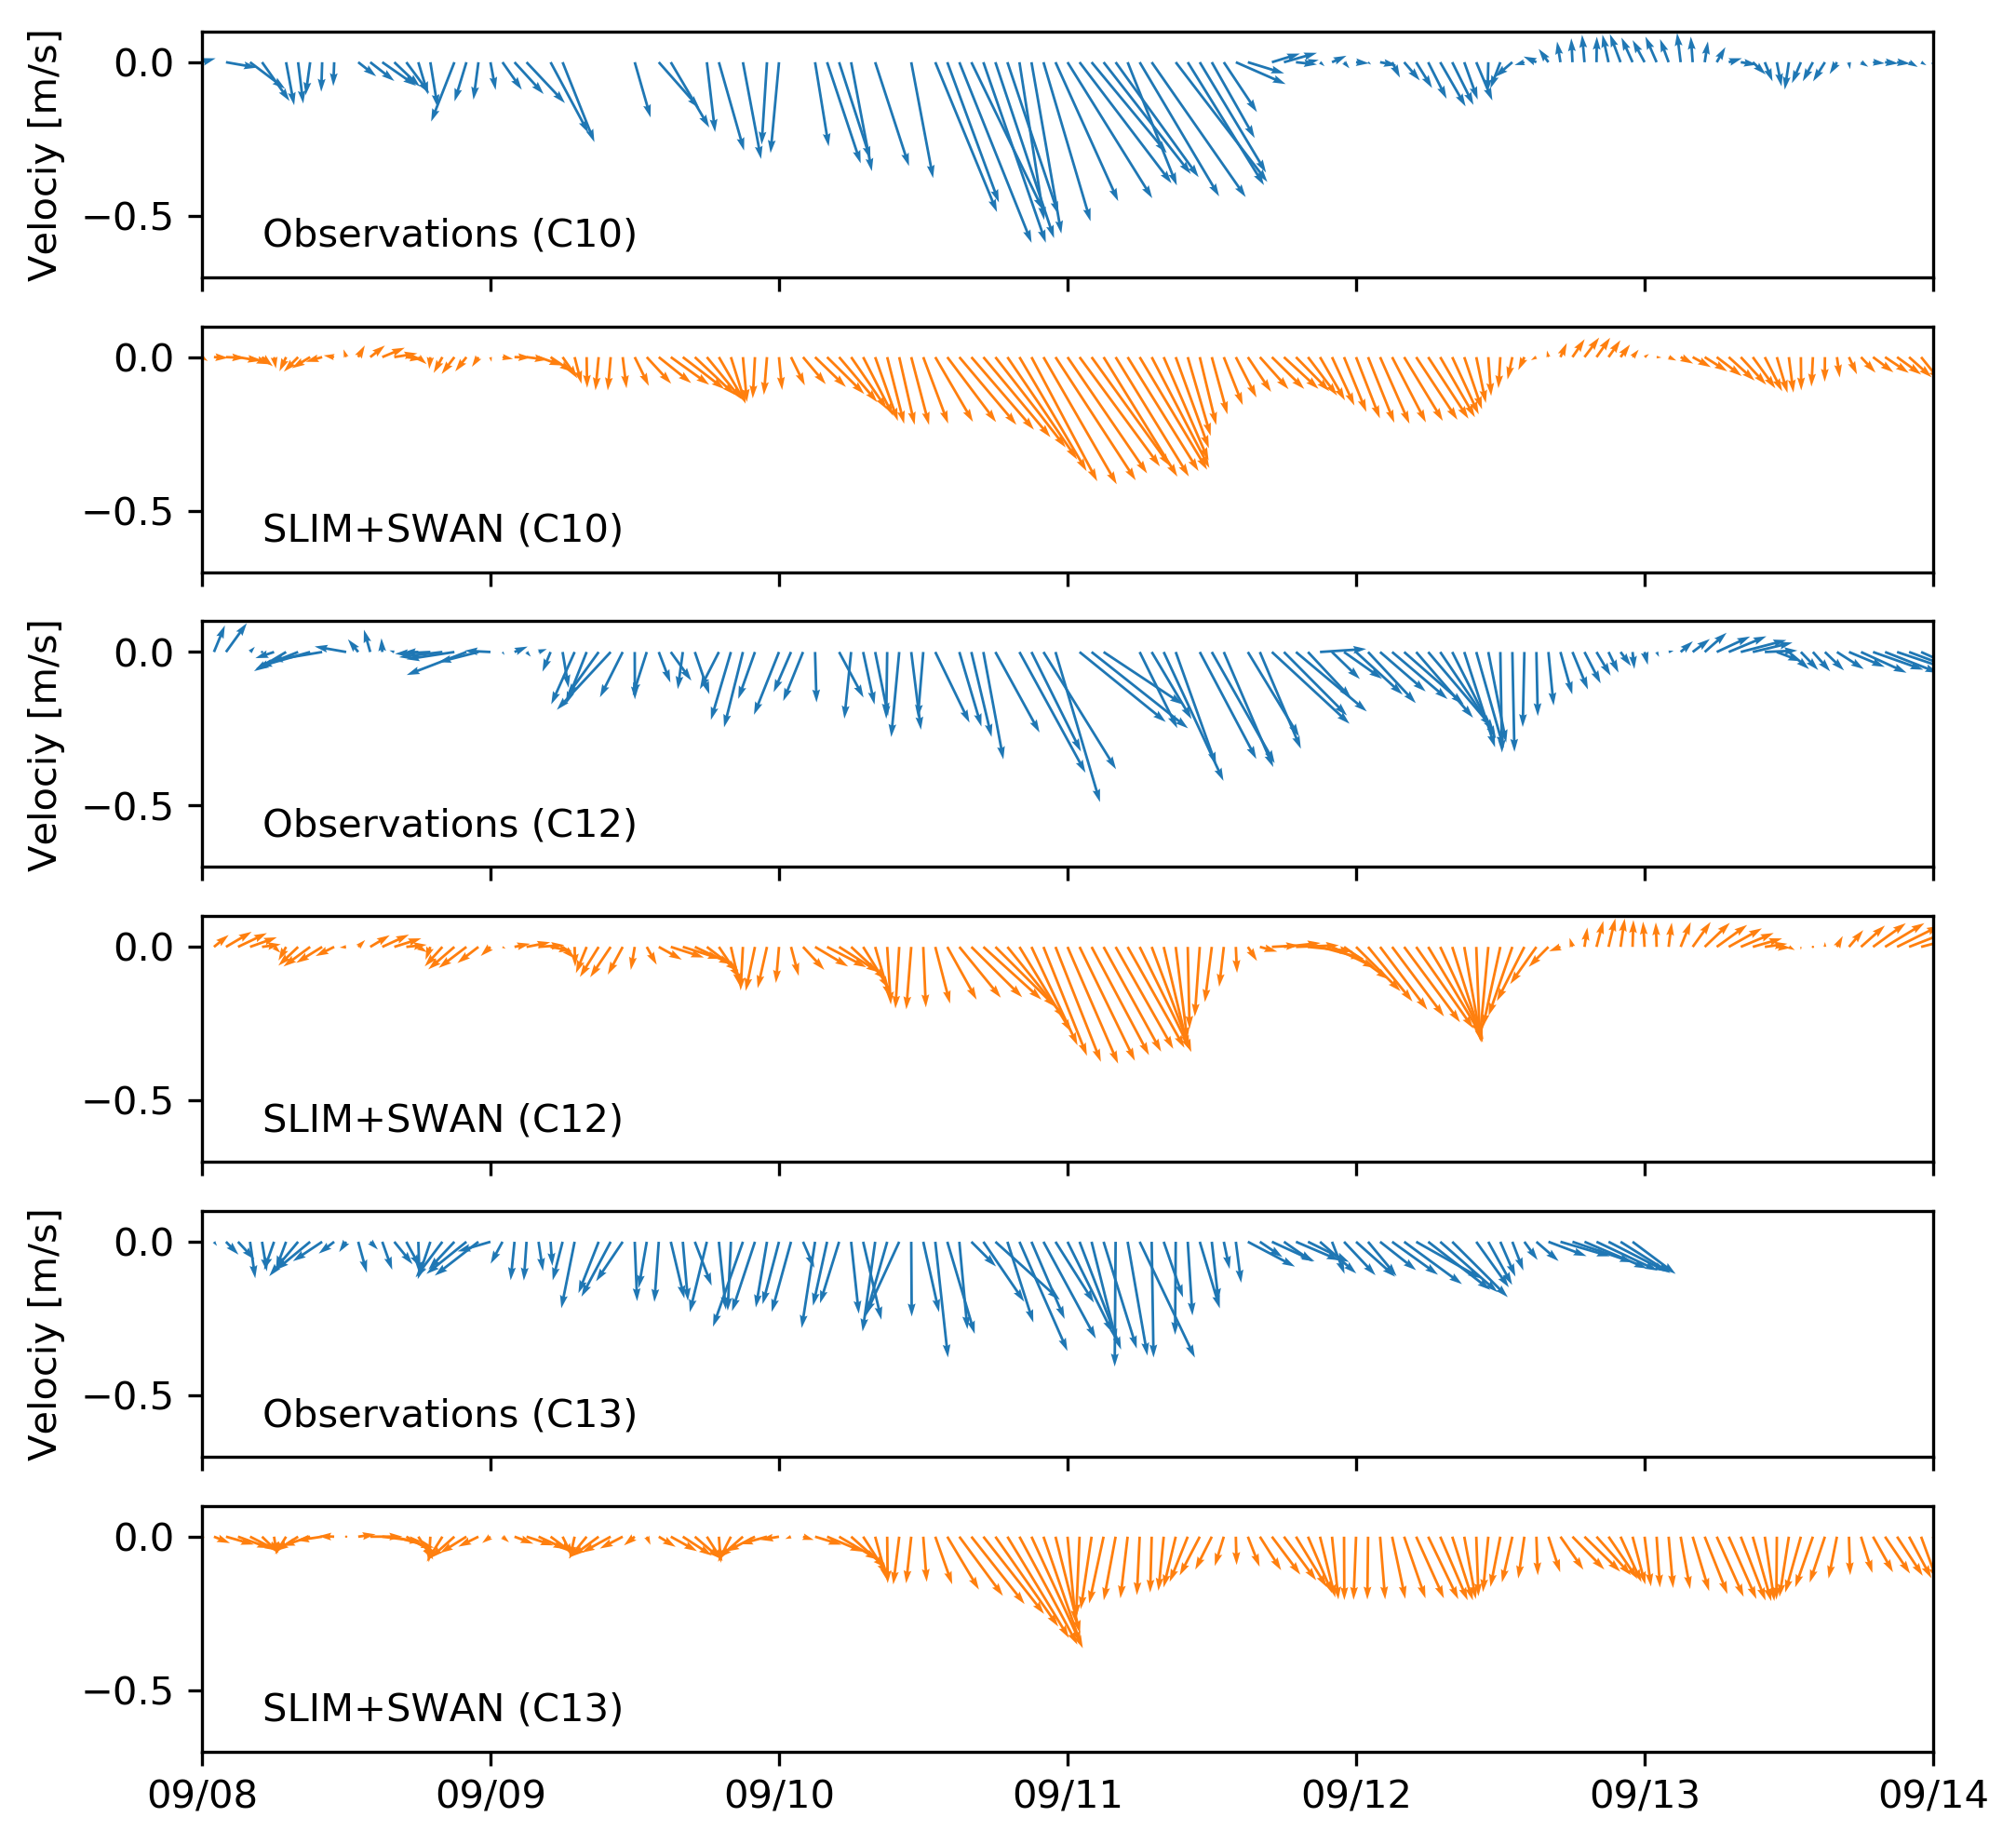
\includegraphics[width=\textwidth]{chapters/irma/figures/figure_currents_all.png}
    \caption{Comparison of modeled current velocity with observed velocity at the moorings (see Fig. \ref{fig:mesh}B for their location). Modeled current velocities agree well with observations, with a correlation coefficient of 0.87, 0.83 and 0.81 at moorings C10, C12 and C13, respectively. The corresponding veering angles are $5.4^\circ$, $0.07^\circ$ and $10.5^\circ$, respectively.}
    \label{fig:uv}
\end{figure}

The simulated significant wave height agrees well with observations at all buoy locations (Fig. \ref{fig:waves}). The timing of the peak in wave height is well captured at all buoys, while the amplitude is better reproduced on the WFS (buoys 42036 and 42097) with errors below 10\%. The error on the peak amplitude on Florida's eastern shelf is of 13\% and 21\% at buoys 4114 and 4113, respectively. On average, observed significant wave height and wave period are better reproduced on the WFS while wave direction is better captured by the model on Florida's eastern shelf (Table \ref{tab:stat}). The fit is especially good at buoy 41113, where the mostly westward-northwestward wave propagation is less perturbed by Irma's wind field.
\begin{figure}
    \centering
    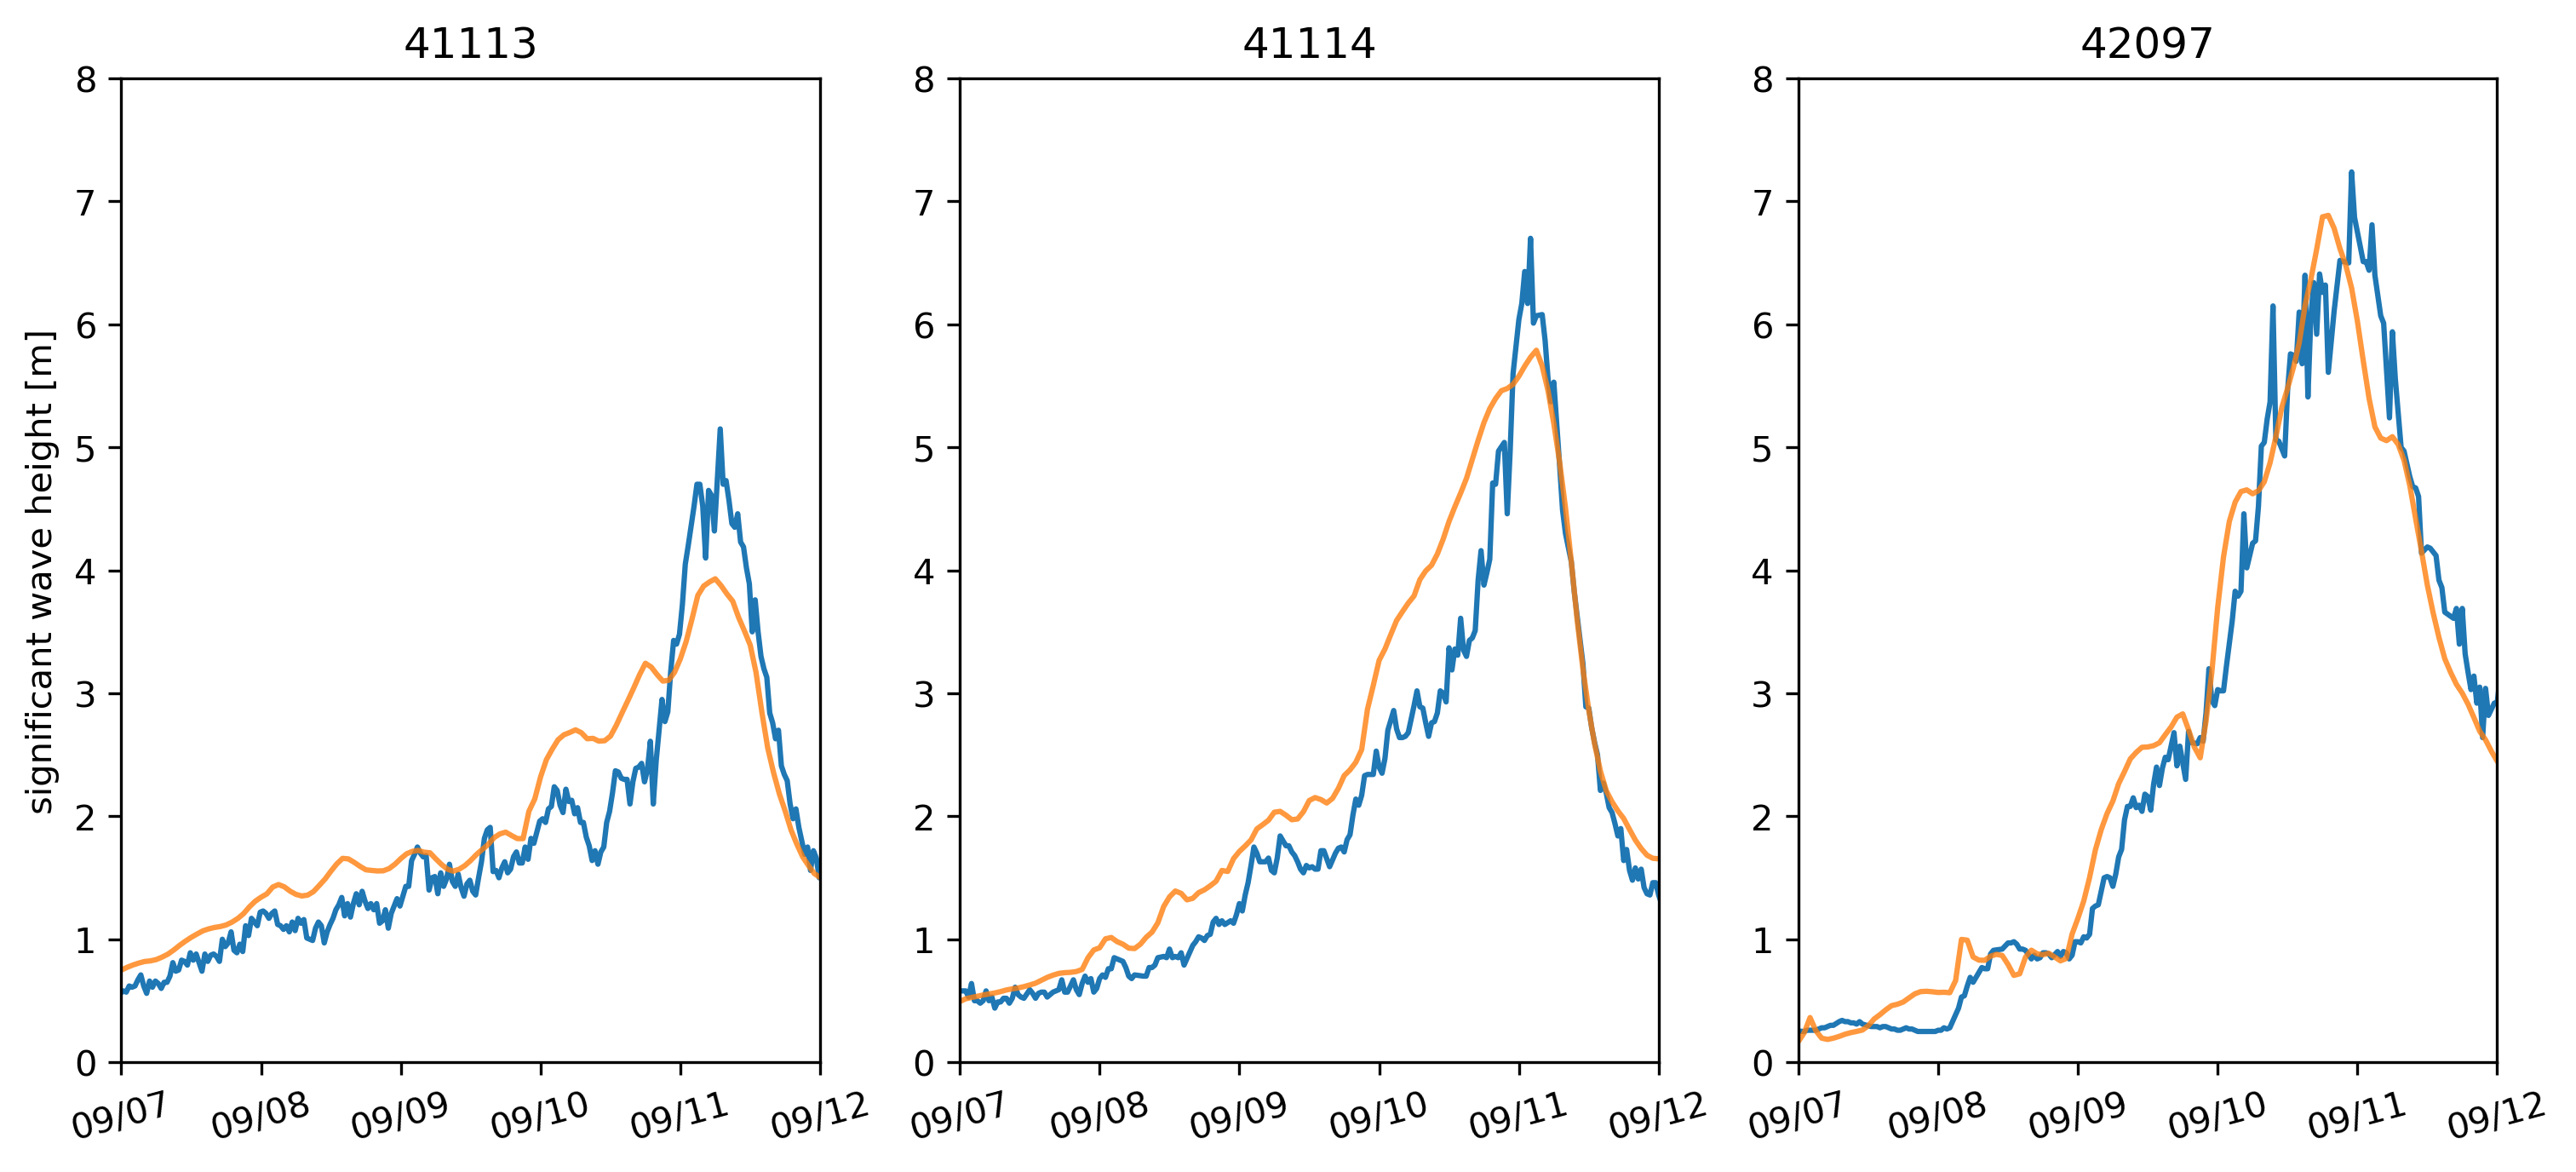
\includegraphics[width=\textwidth]{chapters/irma/figures/hsig_validation.png}
    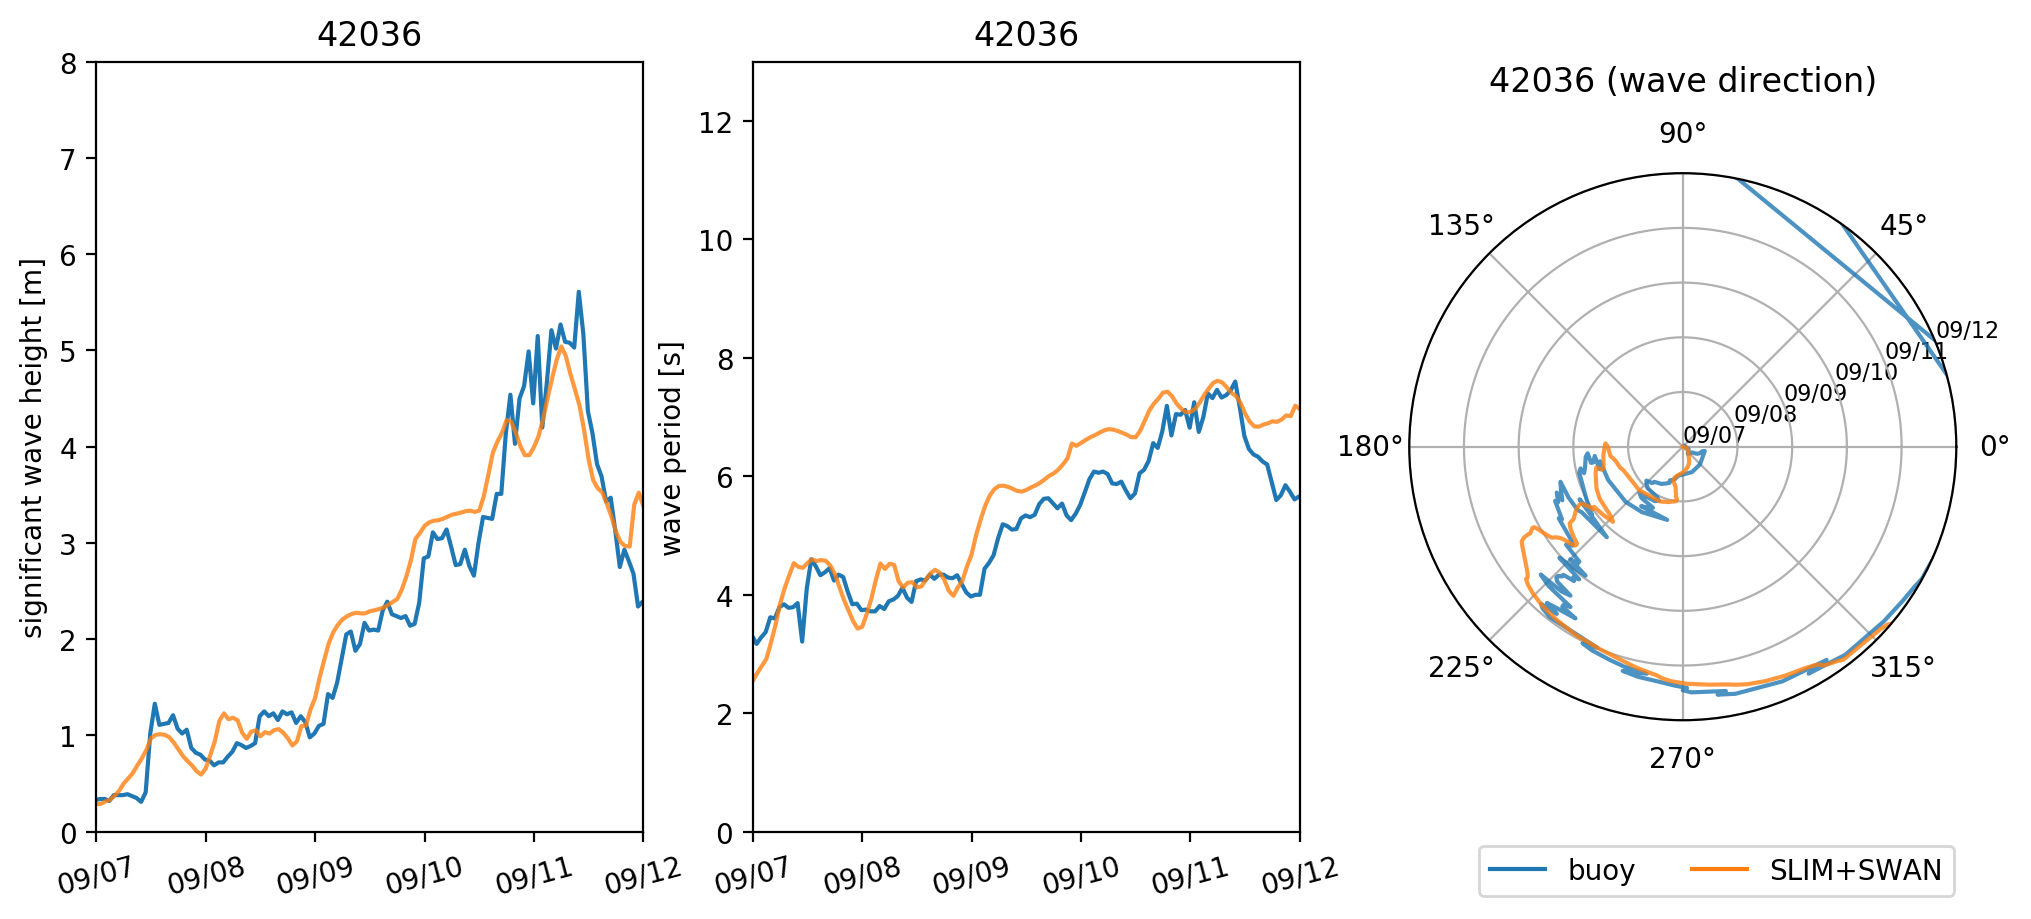
\includegraphics[width=\textwidth]{chapters/irma/figures/wave_validation_42036.png}
    \caption{Comparison of modeled wave parameters with observation at the 4 buoys location (locations shown in Fig. \ref{fig:mesh}B). Overall, the modeled significant wave heights agree well with field measurement (mean error $<25$\%). }
    % As model parameters were calibrated for the Northern Gulf of Mexico, observations are better reproduced at buoys located on the WFS, as illustrated for buoy 42036
    \label{fig:waves}
\end{figure}

\begin{table}
    \centering
    \begin{tabular}{|p{2.3cm}p{2.3cm}p{1.3cm}p{1.3cm}p{1.3cm}|}
        \hline
        \textbf{Station} & \textbf{Variable} & \textbf{Bias} & \textbf{MAE} & \textbf{RMSE} \\
        \hline
        Vaca Key     & sse (m)              & 0     & 0.112 & 0.142 \\
                     & $U_{10}$ (m/s)       & 1.51  & 1.85  & 2.61 \\
                     & $p_\text{atm}$ (hPa) & -0.21 & 0.59  & 1.03 \\ 
        Key West     & sse (m)              & 0     & 0.066 & 0.085 \\
        Virginia Key & sse (m)              & 0     & 0.087 & 0.120 \\
        Naples       & sse (m)              & 0     & 0.099 & 0.180 \\
        \hline
        C10   & $u$ (m/s)           &  0.002 &  0.045 &  0.056 \\
              & $v$ (m/s)           &  0.039 &  0.102 &  0.121 \\
        C12   & $u$ (m/s)           &  0.002 &  0.059 &  0.074 \\
              & $v$ (m/s)           &  0.047 &  0.073 &  0.094 \\
        C13   & $u$ (m/s)           & -0.009 &  0.065 &  0.077 \\
              & $v$ (m/s)           &  0.039 &  0.086 &  0.102 \\
        \hline
        41113 & $H_s$ (m)           &  0.150 &  0.357 &  0.430 \\
              & $T_m$ (s)           &  1.608 &  1.671 &  1.878 \\
              & $\theta_m$ (degree) & -1.555 &  7.036 &  9.250 \\
        41114 & $H_s$ (m)           &  0.361 &  0.424 &  0.560 \\
              & $T_m$ (s)           &  0.899 &  1.506 &  1.594 \\
              & $\theta_m$ (degree) & -8.236 & 14.616 & 22.560 \\
        42036 & $H_s$ (m)           &  0.082 &  0.312 &  0.398 \\
              & $T_m$ (s)           &  0.430 &  0.528 &  0.645 \\
              & $\theta_m$ (degree) & -2.307 & 17.144 & 22.734 \\
        42097 & $H_s$ (m)           &  0.048 &  0.326 &  0.432 \\
              & $T_m$ (s)           &  0.476 &  0.755 &  0.892 \\
              & $\theta_m$ (degree) &  2.538 & 34.760 & 55.892 \\
        \hline
    \end{tabular}
    \caption{Error statistics on the wave-current model outputs as compared to the measured sea surface elevation (sse), eastward and northward depth-average current velocities ($u$,$v$), significant wave height ($H_s$), zero-crossing mean wave period ($T_m$) and mean wave direction ($\theta_m$). Model bias, mean absolute error (MAE), and root mean squared error (RMSE) are listed by variable (unit) and value.}
    \label{tab:stat}
\end{table}

\subsection{Impact of waves on currents and transport}

We evaluated the impact of the RS gradient on the modeled currents during the passage of Irma in the Lower Keys, between Sept. 7 and 13, 2017. First, we computed the maximum difference between currents modeled by SLIM and SLIM+SWAN during this period (Fig. \ref{fig:diff}A). The largest differences in current speed were observed over the reefs, on the shelf break and around islands. They locally reach 1 m/s, with the coupled SLIM+SWAN model yielding the largest amplitudes. The regions where the differences were the largest correspond to areas that experienced large maximum values of the RS gradient {\boldmath$\tau$}$_\text{wave}$ (Fig. \ref{fig:diff}B). These areas of large RS gradient are located on the shelf break and over coral reefs, where important wave energy dissipation occurred through depth-induced wave breaking and bottom dissipation \citep{longuet1964radiation}. This highlights the important protective role of the barrier formed by the offshore reefs, that require a fine spatial resolution to be accurately represented by the model. RS-induced differences in current speed were amplified by the action of the wind stress {\boldmath$\tau$}$_\text{wind}$ (Fig. \ref{fig:diff}C). Wind speeds were larger in the front right quadrant of the hurricane \citep{zedler2009ocean}, yielding larger differences on the right-hand side of the storm trajectory. This is especially clear in the area between the Florida Keys and the Everglades, where relatively small values of {\boldmath$\tau$}$_\text{wave}$ produce current speed differences larger than 0.5 m/s because of the wind stress.

\begin{figure}
    \centering
    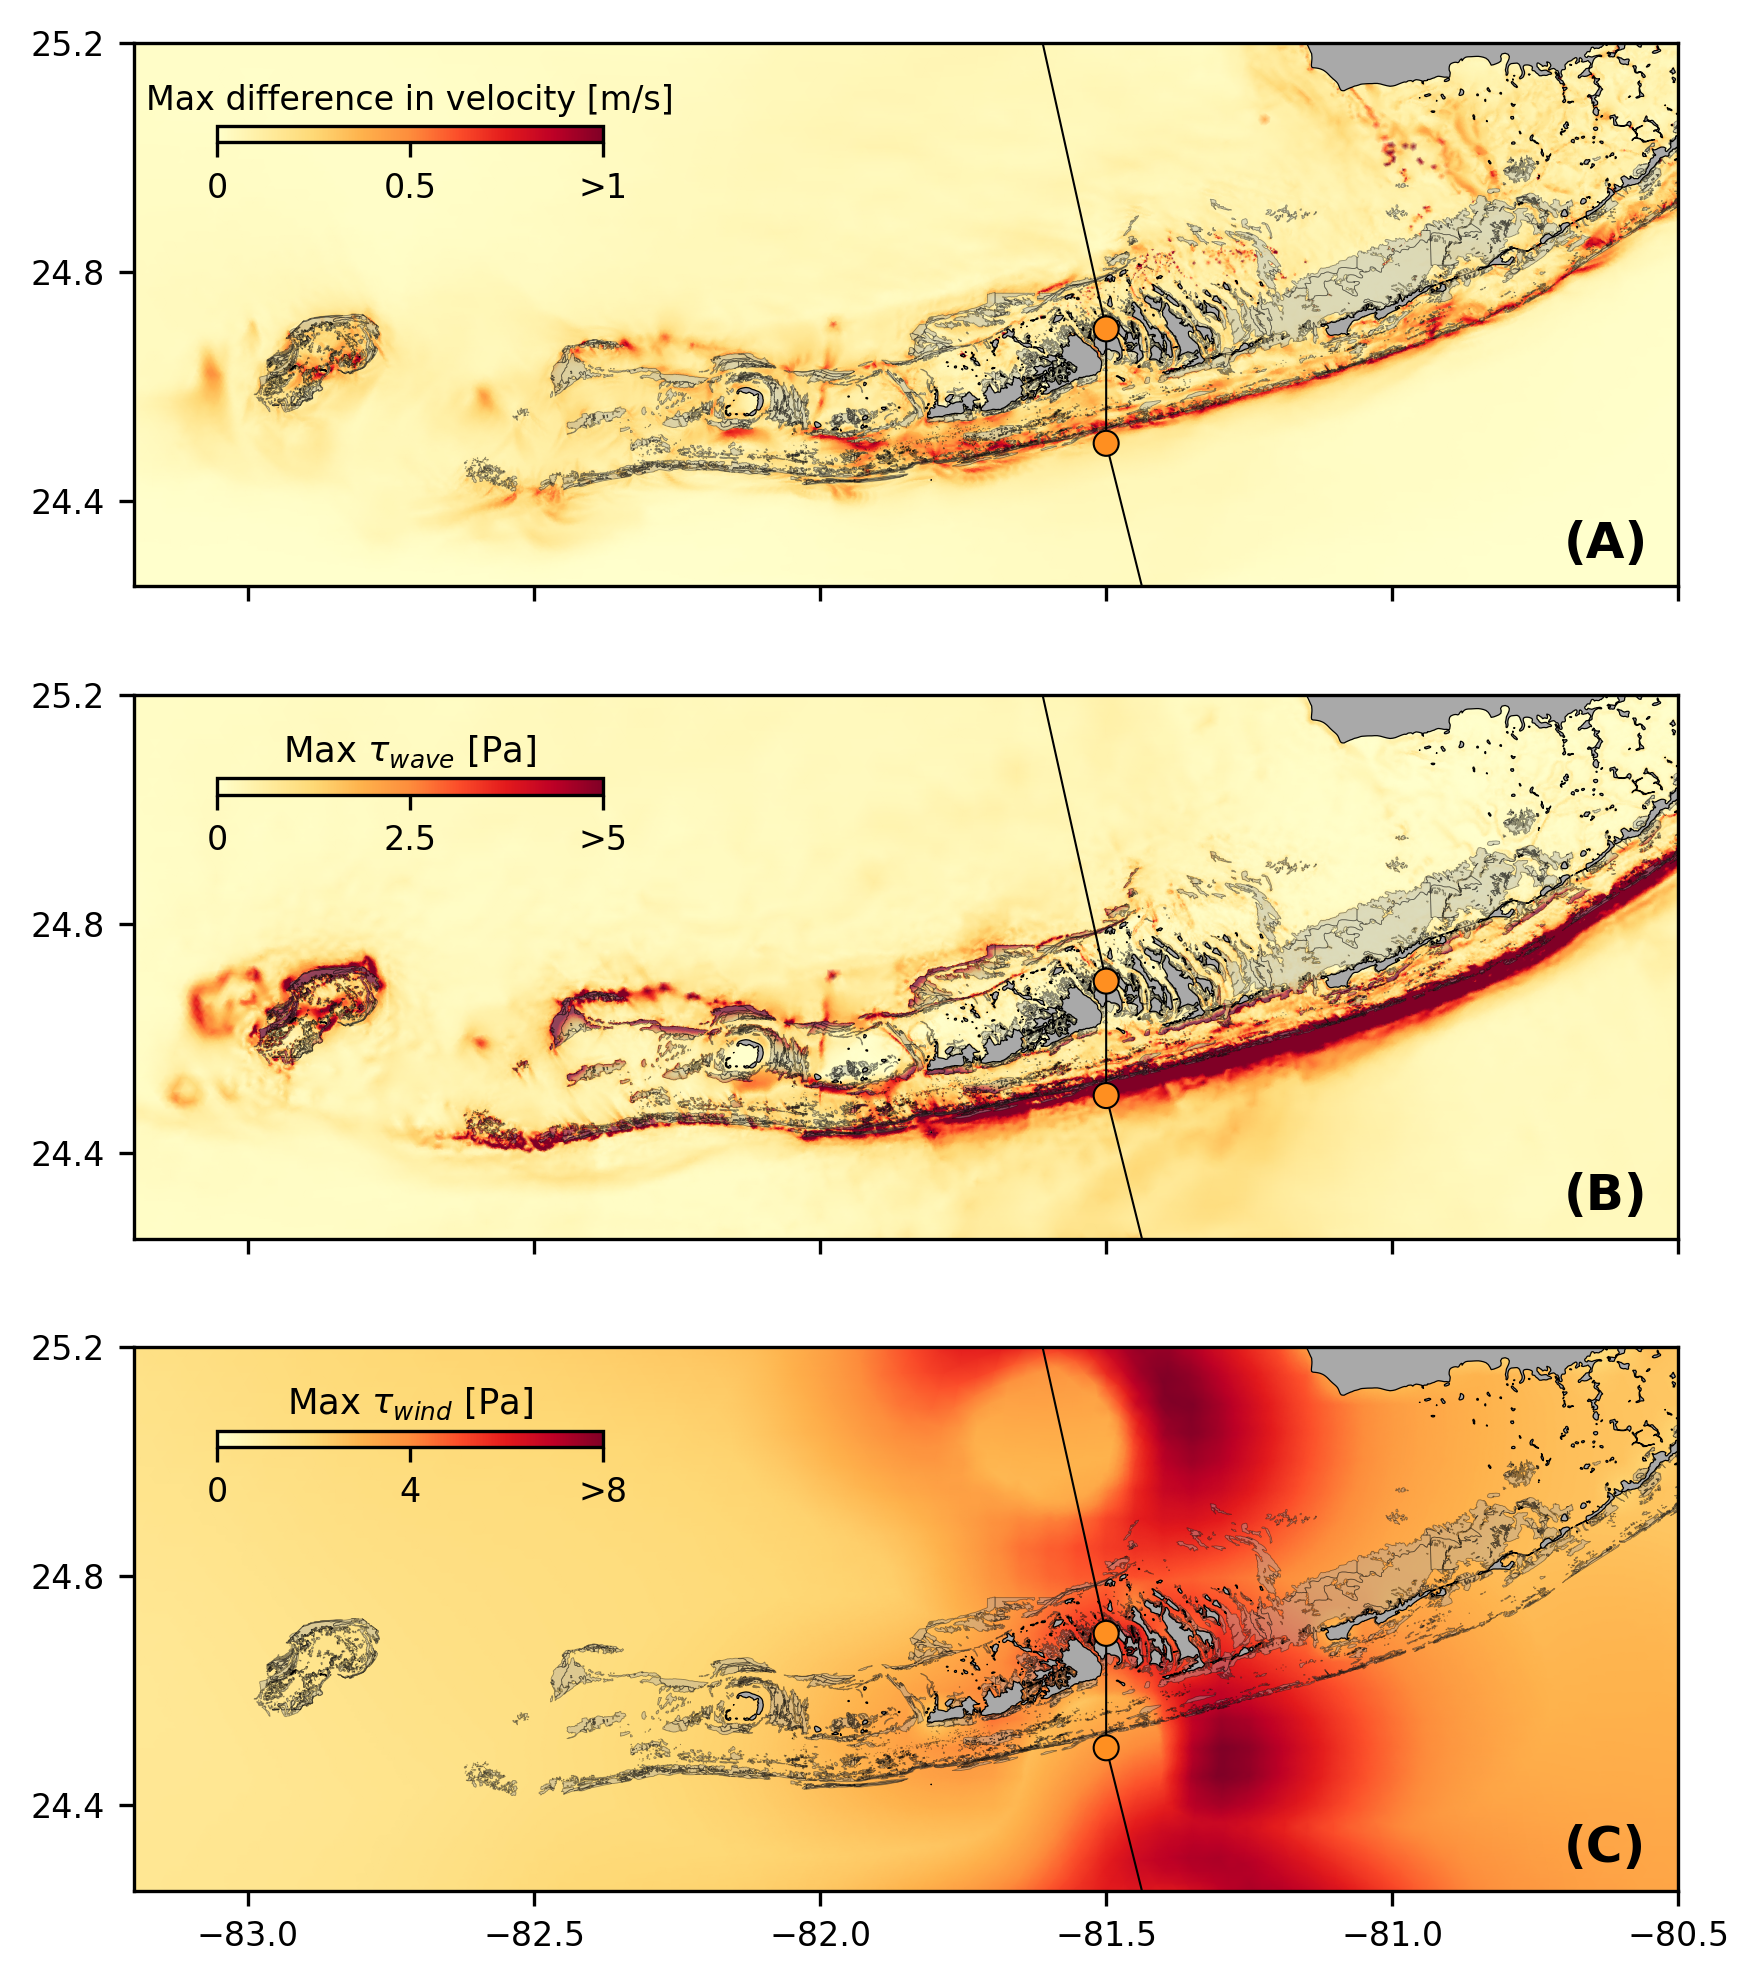
\includegraphics[width=\textwidth]{chapters/irma/figures/max_diff_new.png}
    \caption{(\textbf{A}). Maximum difference between SLIM and SLIM+SWAN currents during the passage of Irma in the Lower Florida Keys; (\textbf{B}) Maximum wave radiation stress gradient {\boldmath$\tau$}$_\text{wave}$ and (\textbf{C}) maximum wind stress {\boldmath$\tau$}$_\text{wind}$ (\textbf{C}) generated by the hurricane. Radiation stress gradient yields currents speed differences reaching 1 m/s, especially over offshore reefs.}
    \label{fig:diff}
\end{figure}

Our results suggest that the RS gradient alone can deflect particle trajectories by up to 1 km on the inner shelf and 5 km on the outer shelf (Fig. \ref{fig:traj}A,B). The RS mainly affects transport processes during the passage of the hurricane, as the distance between particle cloud advected by SLIM and SLIM+SWAN currents remains roughly constant afterwards. The Stokes drift, however, has a longer-lasting effect on the particle trajectories on the outer shelf. When adding a Stokes drift component to the Eulerian currents, the distances between the particle cloud centers keeps increasing during 2 days after the passage of Irma (Fig. \ref{fig:traj}B). Under the effect of the Stokes drift, particles from the outer shelf can be moved inshore on the passage of the hurricane. This motion is less pronounced for particles that are advected by Eulerian currents only. The particle cloud thus moves quickly northeastward under the action of the FC. After 2 days, the particles advected inshore under the action of the Stokes drift are in turn entrained by the FC and the distance between the clouds of particles starts decreasing. The impact of the Stokes drift on particle motion appears to be five times larger than the one of the RS on the inner shelf (Fig. \ref{fig:traj}A). However, both processes yield a similar impact on the particle trajectories at the moment of the passage of Hurricane Irma on the outer shelf (Fig. \ref{fig:traj}B).

Taking wave-currents interactions into account appears to significantly impact the modeled Stokes drift (Fig. \ref{fig:traj}C,D). Our results suggest that neglecting the wave-current coupling when computing the Stokes drift in storm conditions can yield deflections of the particle trajectories by up to 5 km on both the inner and outer shelves. On the outer shelf, differences in particle trajectories mostly appear during the two days following the passage of the hurricane. This is explained by the stronger shoreward component of the coupled SLIM+SWAN Stokes drift compared to the uncoupled one. On the inner shelf, however, differences in particle trajectories of up to 5 km occur at the moment of the passage of Hurricane Irma. The distance between the particle clouds then stabilizes directly after the passage of the hurricane.

% Milan: Table in complement of graph for comparison of trajectories ?

\begin{figure}
    \centering
    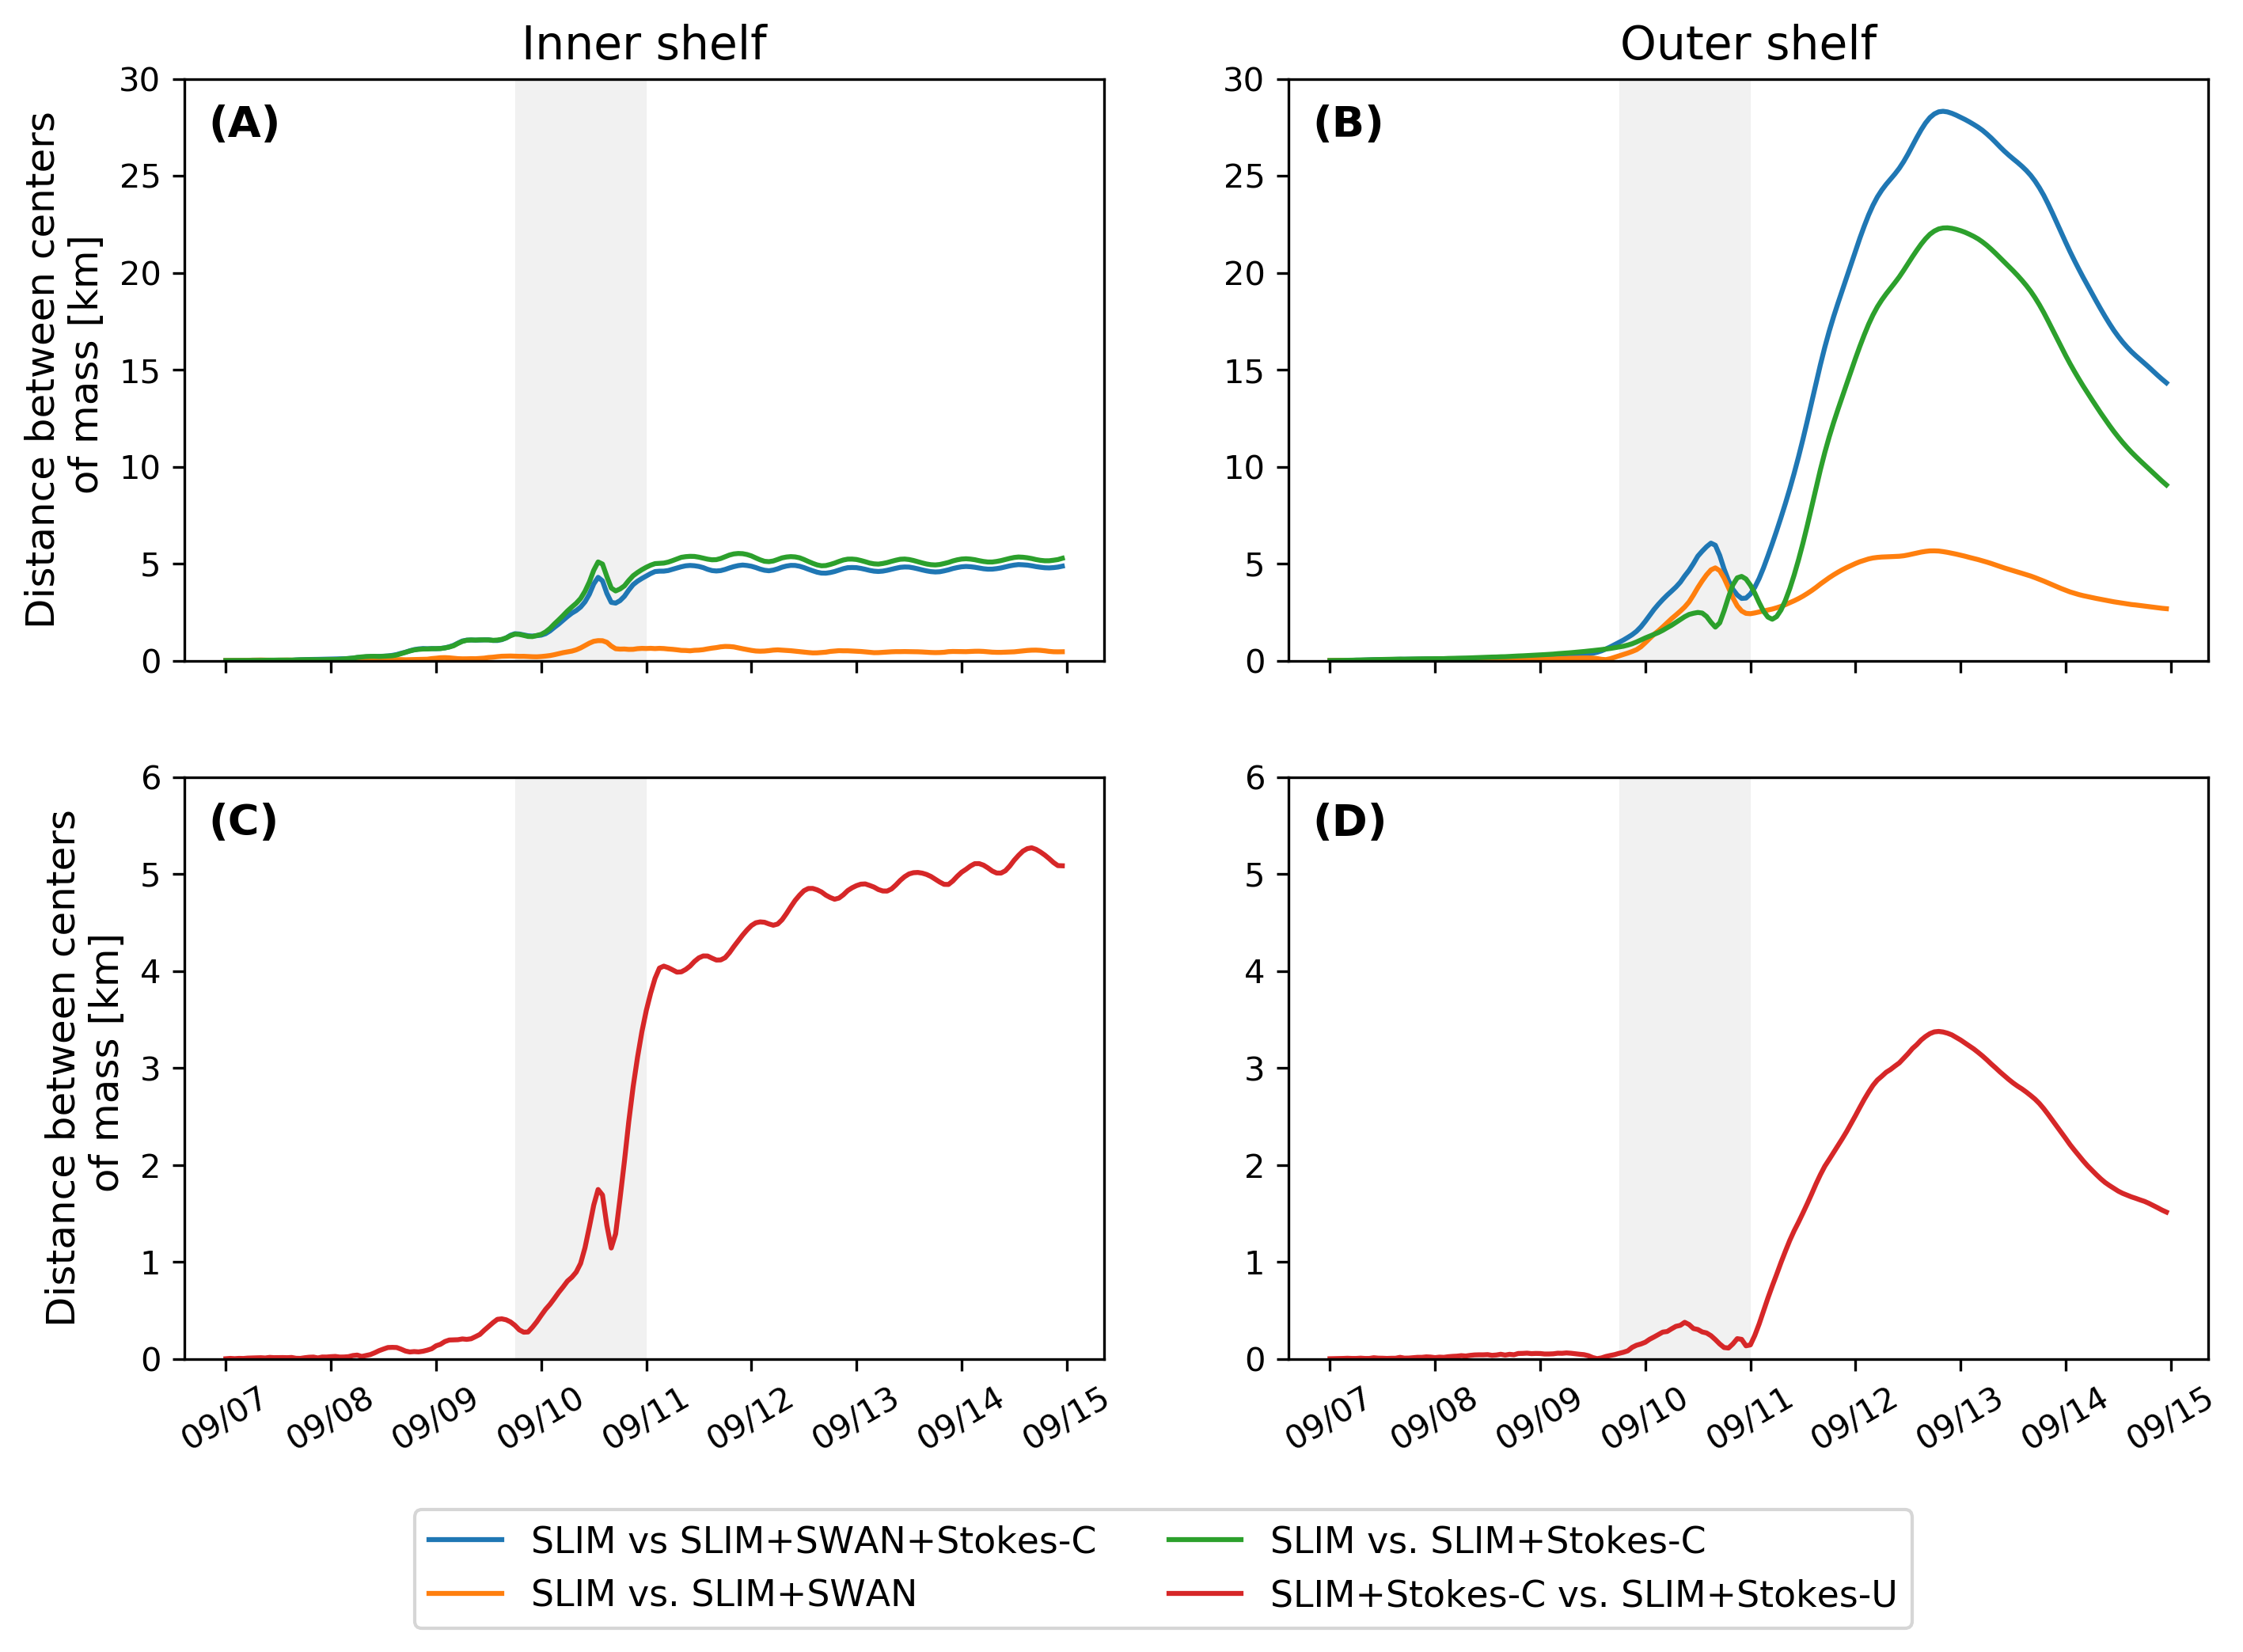
\includegraphics[width=.99\textwidth]{chapters/irma/figures/trajectory_comparisons.png}
    \caption{Difference between the centers of mass of the particle clouds released from the regions highlighted in Fig. \ref{fig:init} and advected by the different combinations of Eulerian currents and Stokes drifts described in Table \ref{tab:summary} \modif{In the top panels, the trajectories of particles advected by Eulerian currents from an uncoupled SLIM run are compared with trajectories obtained with Eulerian currents and Stokes drift from a coupled SLIM+SWAN run (green); Eulerian currents from a coupled SLIM+SWAN run (orange); and Eulerian currents from and uncoupled SLIM run and Stokes drift from a coupled SLIM+SWAN run on the inner (\textbf{A}) and outer shelves (\textbf{B}). The bottom panels show the comparison of the trajectories of particles advected by Eulerian currents from an uncoupled SLIM run and Stokes drift from coupled and uncoupled model runs on the inner (\textbf{C}) and outer (\textbf{D}) shelves.}}
    \label{fig:traj}
\end{figure}

% \begin{figure}
%     \centering
%     \includegraphics[width=.98\textwidth]{fig/dispersion.png}
%     \caption{Dispersion of particles with different velocity fields $\rightarrow$ not sure to know what to say about that...}   
%     \label{fig:dispersion}
% \end{figure}

% === DISCUSSION === %
\section{Discussion}
% SUMMARY
The coupled SLIM+SWAN model correctly reproduced the hydrodynamics and wave dynamics during Hurricane Irma. Such good agreement with field measurements could only be achieved using accurate forcings and adequate wave parameterizations. By comparing coupled and uncoupled model runs, we showed that neglecting wave radiation stress gradient can induce differences of up to 1 m/s in modeled current velocities. The radiation stress gradient during the hurricane was especially large over the shelf break, where waves are strongly dissipated by the offshore coral reef barrier. The radiation stress gradient alone can deflect drifting particles by up to 5 km during the passage of the hurricane. The impact of the Stokes drift dominates the effects of the radiation stress gradient on transport processes, except during the passage of the hurricane, when both contributions are similar on the outer shelf. The Stokes drift induces a shoreward transport during the passage of the hurricane that moves particles towards  the inner shelf, and hence away from the FC. Finally, neglecting wave-current interactions when computing Stokes drift leads to variations of up to 5 km in modeled trajectories on the passage of the hurricane.

The coupled wave-current model correctly reproduced the timing of the observed storm surges and captured the elevation peaks with a 15\% accuracy at every tide gauge except Virginia Key. Such accuracy is key to predict the damages caused by the hurricane, as they were mostly due to the storm surge and  high waves \citep{xian2018brief}. Furthermore, by using a high-resolution model, we can explicitly reproduce the circulation between all the reefs and islands of the Florida Keys. The fine-scale details of the storm surge, and hence the associated risk, are thus accurately represented. In addition to accurately capturing positive surges, the model also reproduced the observed negative surge in Naples. This result is of interest from a biological point of view as negative surges, although less studied, affect water exchanges between the estuaries and the coastal ocean and disturb the benthic ecosystems \citep{liu2020impacts}. Such rapid decrease in water level followed by a positive surge cause massive freshwater inflows, causing a significant decrease in water salinity \citep{wachnicka2019hurricane}. Surface waters are also significantly impacted by storms and hurricanes through induced cooling, upwelling and mixing \citep{varlas2020investigating}, but these processes were not accounted for in our model.

Strong currents such as the Gulf Stream affect waves through refraction over gradients in current velocity, shoaling and breaking of opposing waves or lengthening of following waves \citep{hegermiller2019wave}. Under hurricane conditions, these interactions can cause numerical instabilities in the wave model if the parameterizations are not appropriate and the model resolution not sufficient. \cite{hegermiller2019wave}, for instance, used a 5-km model grid and 48 directional bins to capture spatial gradients in wave height induced by wave-currents interactions in the Gulf Stream during Hurricane Matthew (2016). We followed these guidelines when defining the coarsest mesh resolution as the wave model spectral discretization. Boundary conditions and directional spreading of the incident waves also play a significant role when modeling wave-current interactions at meso- and submesoscales \citep{villas2020wave}, which motivated our choice of imposing full spectra on the boundary of the wave model instead of bulk parameters.

Tropical cyclones interact with the Gulf Stream and the FC through cooling and mixing of the upper ocean. These interactions can momentarily disrupt these currents and cause a significant reduction of their transport \citep{oey2007hurricane,ezer2017observations,ezer2020long}. As a 2D barotropic model, SLIM does not explicitly capture the vertical structure of the FC and Gulf Stream. Furthermore, a coupling with an atmospheric model would be required to represent heat fluxes between the upper ocean and the hurricane. However, we argue that a 2D model is sufficient for the scope of this study, that focuses on nearshore processes on the shelf and the shelf slope. Furthermore, by coupling the model with HYCOM, SLIM is able to represent indirectly the baroclinic features such as the meandering of the FC and eddie formation \citep{frys2020fine}. Furthermore, using a 2D model allows us to capture the impact of wave-current interactions on transport processes at the reef scale in the topologically complex coastal system of the FRT. Such a fine resolution is key to estimate the amount of wave energy dissipated over offshore reefs and accurately capture the generated RS gradient.

%Finally, SWAN default parameterizations for wind energy input and whitecapping caused numerical instabilities by overestimating wave growth and steepness on the boundary of the Gulf Stream on the passage of Irma. This overestimation was solved by using the parameterization of \cite{siadatmousavi2011evaluation}. The parameters used in this study were calibrated on the Northern Gulf of Mexico conditions, which might explain that our model better reproduces wave parameters at buoys located on the WFS. However, these calibrated parameters might underestimate wind-induced wave growth on Florida's eastern shelf. Consequently, incident wave do not receive enough energy to grow after breaking on the bank boundary, leading to an underestimation of the significant wave height at buoys located on Florida's eastern shelf. A more extensive calibration study might therefore be necessary to further improve the agreement with field measurements on both sides of Florida. Nonetheless, as this study focuses on the wave produced by Irma, which made landfall on the West coast of Florida, the use of parameterizations calibrated for the Gulf of Mexico seems reasonable.

The RS gradient significantly impacts currents during the passage of the hurricane. It can induce differences of up to 1 m/s in the current speed on the shelf break. In this region, waves are strongly dissipated due to action of depth-induced breaking and bottom dissipation on coral reefs. This link between wave breaking, RS gradient and wave-induced nearshore currents is consistent with previous studies on wave-current dynamics during storms \citep{mao2017dynamics,mao2018wave,mao2020particle}. Furthermore, our results highlight the protective role of coral reefs against strong incoming waves \citep{lowe2005spectral}, which requires a sufficiently fine spatial resolution to be explicitly represented in the model. As wave energy mostly dissipates on the shelf break, the impact of the RS gradient on transport processes is 5 times larger on the outer shelf. In the sheltered area of the inner shelf, wave impact on transport processes is dominated by the Stokes drift. Trajectory deflection under the influence of wave-induced motions mostly occurs at the moment of the passage of the hurricane on the inner shelf. After that moment, the distance between the clouds of particles remained roughly constant through time. On the outer shelf, RS and Stokes drift have a similar impact on transport processes at the moment of the passage of the cyclone and deflect particle trajectories by up to 5 km. However, by inducing shoreward transport, the Stokes drift delayed the advection of particles by the FC, therefore causing differences in trajectories of up to 20 km during the days following the passage of the hurricane. The dominance of the Stokes drift on particle transport in storm conditions was also observed in Lake Michigan by \cite{mao2020particle}. Finally, neglecting wave-current coupling in Stokes drift computation leads to differences in modeled trajectories of the order of 5 km on both the inner and the outer shelves. This fact, coupled with the impact of RS-induced currents strongly advocates for the use of coupled wave-current models when studying transport processes in storm conditions.

%Due to the dissipation of incoming waves on the reefs, wave impact during Irma is different on the inner and outer shelves. It is less important on the inner shelf because of the sheltering of the inner shelf due to reefs and islands as well as wave breaking on the shelf break. The inner shelf hence experiences weaker waves and currents, inducing weaker and more localized transport. Furthermore, the impact of winds on waves is reduced in shallower areas under the action of depth-induced breaking. This might explain why differences between particle trajectories stabilize on the inner shelf just after the passage of Hurricane Irma. However, the Florida Keys still experienced strong winds after the passage of the core of the hurricane, which generated high waves in the deeper areas. This might explain why the differences between the modeled trajectories kept increasing on the outer shelf under the action of strong Stokes drift up to two days after the passage of the hurricane.

\section{Conclusion}

We developed a coupled wave-current model to study the impact of waves on transport processes during Hurricane Irma. In order to accurately represent the wind and pressure profiles of the hurricane, we built hybrid fields by combining coarser ERA-5 data with high-resolution H*Wind data for the wind speed and idealized Holland profiles for the pressure. Comparing these hybrid profiles with field observations showed that they were better at reproducing the observed central depression of the hurricane as well as the peak in wind speed than ERA-5 data. Using these hybrid fields as forcings, our coupled model accurately reproduced the storm surge at tide gauge locations and produced currents and wave parameters in good agreement with field observations. The modeled currents and Stokes drift were then used to evaluate the impact of wave-current coupling on the modeled trajectories of passive drifters on the passage of the hurricane through the Florida Keys. Our results show that waves had a significant impact on heavy-wind transport processes and caused deflections of the drifters trajectories by more than 20 km on the outer shelf.

Despite its good agreement with observations, our model could be further refined by improving the representation of wind-wave interactions. In particular, we did not consider the momentum loss due to the action of surface waves, which can lead to overestimations of the momentum flux from the atmosphere to the ocean under hurricane conditions. Our model could therefore be further improved by using a wave-dissipative stress instead of the full wind stress as the momentum flux from the atmosphere to the ocean. As a 2D barotropic model, SLIM does not explicitly represent heat fluxes between the ocean and the atmosphere and the vertical structure of the ocean. However, our study focused on relatively shallow and vertically homogeneous coastal waters using a reef-scale resolution throughout the whole FRT. Such fine resolution allows to explicitly represent wave dissipation over coral reefs and is only achievable using a 2D model due to computational resource limitations.

Wave coupling needs to be taken into account during heavy-wind events but not necessarily in milder conditions. While the RS gradient plays an important role and can lead to differences of up to 5 km, the Stokes drift is about 4 times more intense and is thus the most important wave-induced transport process. Nonetheless, neglecting wave-current coupling through RS when modeling Stokes drift leads to differences of up to 5 km in predicted drifter trajectories. Such discrepancies reveal the strong influence of wave-current interactions on transport under storm conditions. This study brings new insight on the impact of waves on the transport processes nearshore during a tropical cyclone. Due to its fine spatial resolution, our coupled wave-current model can be used to accurately represent the dispersal of pollutants, sediments or larvae in topologically complex coastal areas in heavy-wind conditions.  

%%%%%%%%%%%
%
%%%%%  
%%%
  \mychapter{Conclusions and perspectives} \label{chap:conclusion}
  \section{Conclusions}
In this thesis, we have developed a modeling framework to better understand the propagation and onset of the SCTLD, as well as the impact of major hurricanes on transport processes over coral reefs. Our model had to be able to accurately capture ocean circulation patterns at different scales to study transport processes in the FCR. First, the large-scale Loop Current/Florida Current system had to be accurately reproduced to correctly capture its impact on eddy formation near the DRTO and the Florida Keys. Second, the model had to reproduce ocean circulation at the reef-scale to capture the recirculation and acceleration of currents between reefs and islands. This was performed by coupling the multi-scale ocean model SLIM to a connectivity-based epidemiological model (chapter \ref{chap:sctld}), a sediment transport model (chapter \ref{chap:onset}) and a spectral wave model (chapter~\ref{chap:irma}).

Our coupled hydro-epidemiological model reproduced the observed propagation of the SCTLD through the FRT by representing the transport of its causative agent within neutrally buoyant material driven by mean barotropic currents. It confirmed the result of previous ex-situ studies that showed evidence of waterborne transmission of the SCTLD with an average transmission time of the order of 10 days. Furthermore, by using coral resistance to the disease as a parameter, our model results suggested that, on average, corals had a rather low resistance against the disease. This confirmation of experimental results by model results illustrates the important potential of models in evaluating hypotheses derived from field observations on large scale systems. As such, models informed by and confronted against field knowledge \citep{foster2012connectivity} are a powerful tool to inform the management of complex ecosystems such as the FCR.

This epidemiological model was then used to build networks of potential exchanges of disease agents between $\sim 1.6\times10^4$ sub-reef areas composing the FRT during a period of three years. The analysis of these networks showed that exchanges from the Marquesas to the DRTO were interrupted during most of 2020. This interruption was likely linked to eddy activity near the DRTO and was consistent with the apparent stalling of the outbreak in the region in 2020. This confirms the role played by the Loop Current/Florida Current system in the control of the connectivity pathways in the Florida Keys and the DRTO. Furthermore, sub-reefs predicted to be more vulnerable to SCTLD in the disease networks were consistent with the observed geographic distribution of diseased corals in the DRTO. This further highlights that the modeled hydrodynamics is highly explanatory of the propagation of the disease.

The results of chapters \ref{chap:sctld} and \ref{chap:drto} show that our high-resolution biophysical model is a valuable tool to understand the spread of SCTLD in Florida. The model successfully reproduced the observed propagation of the disease in 2018-2019 and allowed us to link the observed stalling of SCTLD to observable hydrodynamic features. Furthermore, the model allowed us to deduce potential characteristics of the disease agent and its vector. This highlights the potential of biophysical models to understand the driving mechanics of ongoing marine disease outbreaks. Furthermore, metrics such as the vulnerablity and source indicators developed in chaper \ref{chap:drto} could be useful to predict and/or mitigate the spread of SCTLD in other territories of the Caribbean.

Using a sediment transport model, we investigated the impact of the PMDDP on the onset of the SCTLD outbreak in 2014. Our results suggest that the dredging operations had close to no direct impact at Virginia Key monitoring site, identified as the reef from which the disease started its propagation. However, reefs affected earlier could have been infected by chopped rock particles produced by non conventional dredging operations in the channel. Moreover, our epidemiological model suggests that disease propagation from these reefs to Virginia Key was possible. Sediments released by the PDMMP might therefore have initiated one of the worst coral disease outbreaks to date in the Caribbean. These results could have consequences on the planning of future major dredging projects in the area such as the Port Everglade Dredging Project\footnote{https://www.porteverglades.net/construction/harbor-improvements/, last consulted on February 12, 2022}. FCR is routinely suffering from important anthropogenic stresses caused by the intense activity of the area of Miami. Hence, coastal developments harm coral reefs in two ways: first, by increasing water turbidity and sedimentation during the dredging, and then by causing an increase in pollution and shipping activities. Such adverse impacts should be taken into account when planning dredging operations. The results of chapter \ref{chap:onset} suggest that the potential to initiate a coral disease outbreak should now also be taken into account when considering future dredging projects.

Finally, we developed a coupled wave-current model to study the impact of Hurricane Irma on transport processes in the Florida Keys. This coupled model correctly reproduced the observed waves and current dynamics during the passage of the hurricane. Furthermore, model results suggest that an important dissipation occurred over coral reefs through depth-induced wave-breaking and bottom friction. This important dissipation produced a large wave radiation stress gradients, which caused differences in modeled velocity of up to 1 m/s between the coupled and uncoupled model runs. However, wave-induced transport was dominated by the Stokes drift, which yielded an impact four times larger than the radiation stress gradient. Results of chapter \ref{chap:irma} strongly advocate for the use of coupled wave-currents to accurately model the dispersal of coral larvae under storm conditions. Although we built the tools to study the impact of hurricane on the exchanges of larvae between reefs by developing the coupled SLIM+SWAN model, we did not evaluate the impact of Irma on coral connectivity by lack of time.

In conclusion, we answered the four research questions defined in chapter \ref{chap:intro}:

\begin{list}{}{%
    % \setlength{\listparindent}{-0.23in}%
    \setlength{\leftmargin}{0in}%
    % \setlength{\itemindent}{-0.23in} 
    }
    \item \textbf{1. How did the SCTLD spread through the FRT ?}
    \begin{list}{}{\setlength{\topsep}{0pt}}
        \item The observed spread of the SCTLD through the FRT was successfully reproduced by modeling the transport of disease agents as neutrally buoyant material within the water column, and by calibrating a connectivity-based epidemiological model with field data. This therefore suggests that the disease spread through waterborne transmission. 
    \end{list}
    \item \textbf{2. What caused the apparent stalling of the propagation of SCTLD ?}
    \begin{list}{}{\setlength{\topsep}{0pt}}
        \item Our results suggest that there was an interruption of hydrodynamic-driven exchanges from the Florida Keys and the Marquesas to the DRTO during most of 2020, which prevented the propagation of disease agents westward. This interruption of the disease connectivity pathways to the DRTO was likely related to the local eddy activity generated by the meandering of the Florida Current.
    \end{list}
    \item \textbf{3. What was the impact of the PMDDP on the onset of the oubreak of SCTLD~?}
    \begin{list}{}{\setlength{\topsep}{0pt}}
        \item Modeling of sediment transport suggests that the chopped rock particles produced by the non conventional dredging activities reached reefs where signs of disease were first reported during the first half of 2014. Furthermore, the modeled disease connectivity suggested that disease propagation from these sites to Virginia Key was possible prior to September 2014. The sediments released by the PMDDP might thus have triggered the onset of the SCTLD outreak at this site.
    \end{list}
    \item  \textbf{4. What is the effect of hurricane-induced wave-current interactions on transport processes and should they be taken into account when modeling the dispersal of coral larvae ?}
    \begin{list}{}{\setlength{\topsep}{0pt}}
        \item Results of a coupled wave-current model suggest that wave-induced transport under storm conditions, dominated by Stokes drift, can yield differences in particle trajectories of up to 20 km. Wave-current interactions should thus be taken into account to accurately model the dispersal of coral larvae during hurricanes.
    \end{list}
\end{list}


\section{Perspectives for future works}

\subsection*{Combining disease and larval connectivity}
All chapters dedicated to SCTLD rely on the concept of connectivity. In this context, connectivity negatively impacts coral reefs as it drives the propagation of disease agents. However, connectivity is actually a double-edged sword. Larval connectivity promotes the resilience of the reef network as it allows the recolonization of disturbed reefs following extreme events such as mass bleaching, hurricanes or disease outbreaks. Larval connectivity is therefore a valuable tool to inform coral reef protection and restoration \citep{botsford2009connectivity,mumby2011reserve}. Identifying reefs that are both good sources and sinks of larvae in the connectivity network indicates the optimal sites for coral outplants in the context of active restoration. Furthermore, knowledge about larval connectivity would allow us to build robust and sustainable networks of connected marine protected areas. As SLIM allows the computation of larval connectivity \citep{thomas2014numerical,frys2020fine,figueiredo2021global}, a possible application of the tools developed in this thesis is the combination of both types of connectivity.  This combined information would allow us to identify reefs that are good larval sources and have low vulnerability to the disease. A possible measure of larval supply to the network is the (weighted) out-degree of reefs in the larval connectivity network, as reefs with strong and numerous outgoing connections in the network are more likely to send many larvae to many connected reefs. Vulnerability to disease can be evaluated using the (weighted) in-degree of reefs in the disease connectivity network, as reefs with strong and numerous incoming connections are more likely to receive more disease agents from many connected reefs. Therefore, reefs with high restoration potential would correspond to reefs with large larval (weighted) out-degree and low disease (weighted) in-degree. This approach have been applied in \cite{holstein2022} and could be further developed in future studies using more complex connectivity metrics such as the PageRank index \citep{frys2020fine}. 

\subsection*{Improving the epidemiological model}
A limitation of the epidemiological model developed in chapter \ref{chap:sctld} is that it uses species-averaged parameters and assumes an uniform distribution of coral species throughout the FRT. The fact that our model correctly reproduced the observed spread of SCTLD for a well-defined range of values of coral resistance to the disease highlights the important impact of this parameter on the propagation of the disease. However, coral susceptibility to SCTLD can significantly vary between species and ranges from highly susceptible (\eg~\textit{Dichocoenia stokesii}, \textit{Meandrina meandrites}) to intermediately susceptible (\eg~\textit{Orbicella faveolata}, \textit{Montastrea cavernosa}) and weakly susceptible (\eg~\textit{Acropora Palmata}, \textit{Acropora cervicornis}). A first improvement could therefore be to consider classes of corals with different susceptibilities and hence use different infection and removal parameter values in the model. Such a development could require the use of more advanced graph theory tools such as multilayer networks \citep{kivela2014multilayer,pilosof2017multilayer}. Furthermore, this improvement would increase the number of variables and parameters of the model, which  would make its calibration more complex. Moreover, this new modeling framework would require estimates of the distribution of the different coral species across the FRT. Compiling this data and deriving realistic estimates would represent a significant challenge. Interestingly, adding species-specific or location-specific parameters in the model would also allow the evaluation of the impact of disease mitigating actions. Lesion treatment using antibiotics could for instance be taken into account in the model by locally reducing the transmission and/or removal parameters. The model parameters could also be made time-dependent as SCTLD progression was reported to slow down during warmer months in the US Virgin Islands \citep{meiling20203d}. Another improvement would be the inclusion of additional processes in the model. For instance, reinfection by SCTLD is currently not possible as corals are "removed" once they are affected by the disease. Given the high mortality of the disease, the "removed" state of the model was assumed equivalent to "dead". However, one might want to discriminate between coral recovery and mortality. Yet, again, adding processes implies an increase in the number of parameters to be calibrated. These modifications could lead to an endemic disease dynamics. 

\subsection*{Better understanding the protective role of corals against storm waves}
Simulation results from the coupled wave-current model suggest that storm waves were significantly dissipated over reefs. The modeled significant wave height under the center of the hurricane reduced from 8 m to $<1$ m over the barrier reef during the passage of the hurricane (Fig. \ref{ccl:swh}). This highlights the important protective role of coral reefs against coastal flooding hazard. Better understanding this role can motivate coral reef restoration efforts. For instance, \cite{ferrario2014effectiveness} estimated that coral reefs could provide wave attenuation comparable to artificial defenses such as breakwaters for a much lower cost. However, modeling the wave-flow dynamics at the reef scale is particularly challenging and requires models that can explicitly represent small-scale nonhydrostatic processes. The smallest scales that models such as SLIM and SWAN can simulate is limited by the intrinsic assumptions in the model formulations, i.e., hydrostatic for SLIM and phase-averaged for SWAN. These assumptions are no longer valid as soon as the horizontal scales of motion become comparable to the vertical scales \citep{marshall1997hydrostatic}. For such situations, it becomes necessary to couple the SLIM+SWAN model with a phase-resolving nonhydrostatic wave-flow model, hence achieving a multi-physics modeling framework. Nonhydrostatic models are more expensive to	 run as they require a much finer spatial resolution of the order of a meter and have a more complex physics. They can therefore often be used only in rather small areas and over short periods of time \citep{fringer2019future}. One promising approach to tackle this issue would be to use machine learning algorithms to locally emulate the dynamics of a complex high-resolution model and hence speed up the computational process \citep{kasim2021building}. Machine learning is based on the principle of extracting information from data, which can either be observational data or high-resolution model outputs, and deriving relationships between datasets without the need for physics-based models. This procedure has recently been applied to ocean modeling and was able to reproduce the temporal and spatial variability of unresolved turbulent processes, when given a smoothed view of the dynamics \citep{bolton2019applications}. Additionally, this multi-physics modeling frameworks could be used to better capture the motion of coral larvae over reef. This would improve the modeled coral connectivity, as the initial motion of larvae over reefs then drives larval transport following mass spawning events, and initiates coral connectivity. 

\begin{figure}
    \centering
    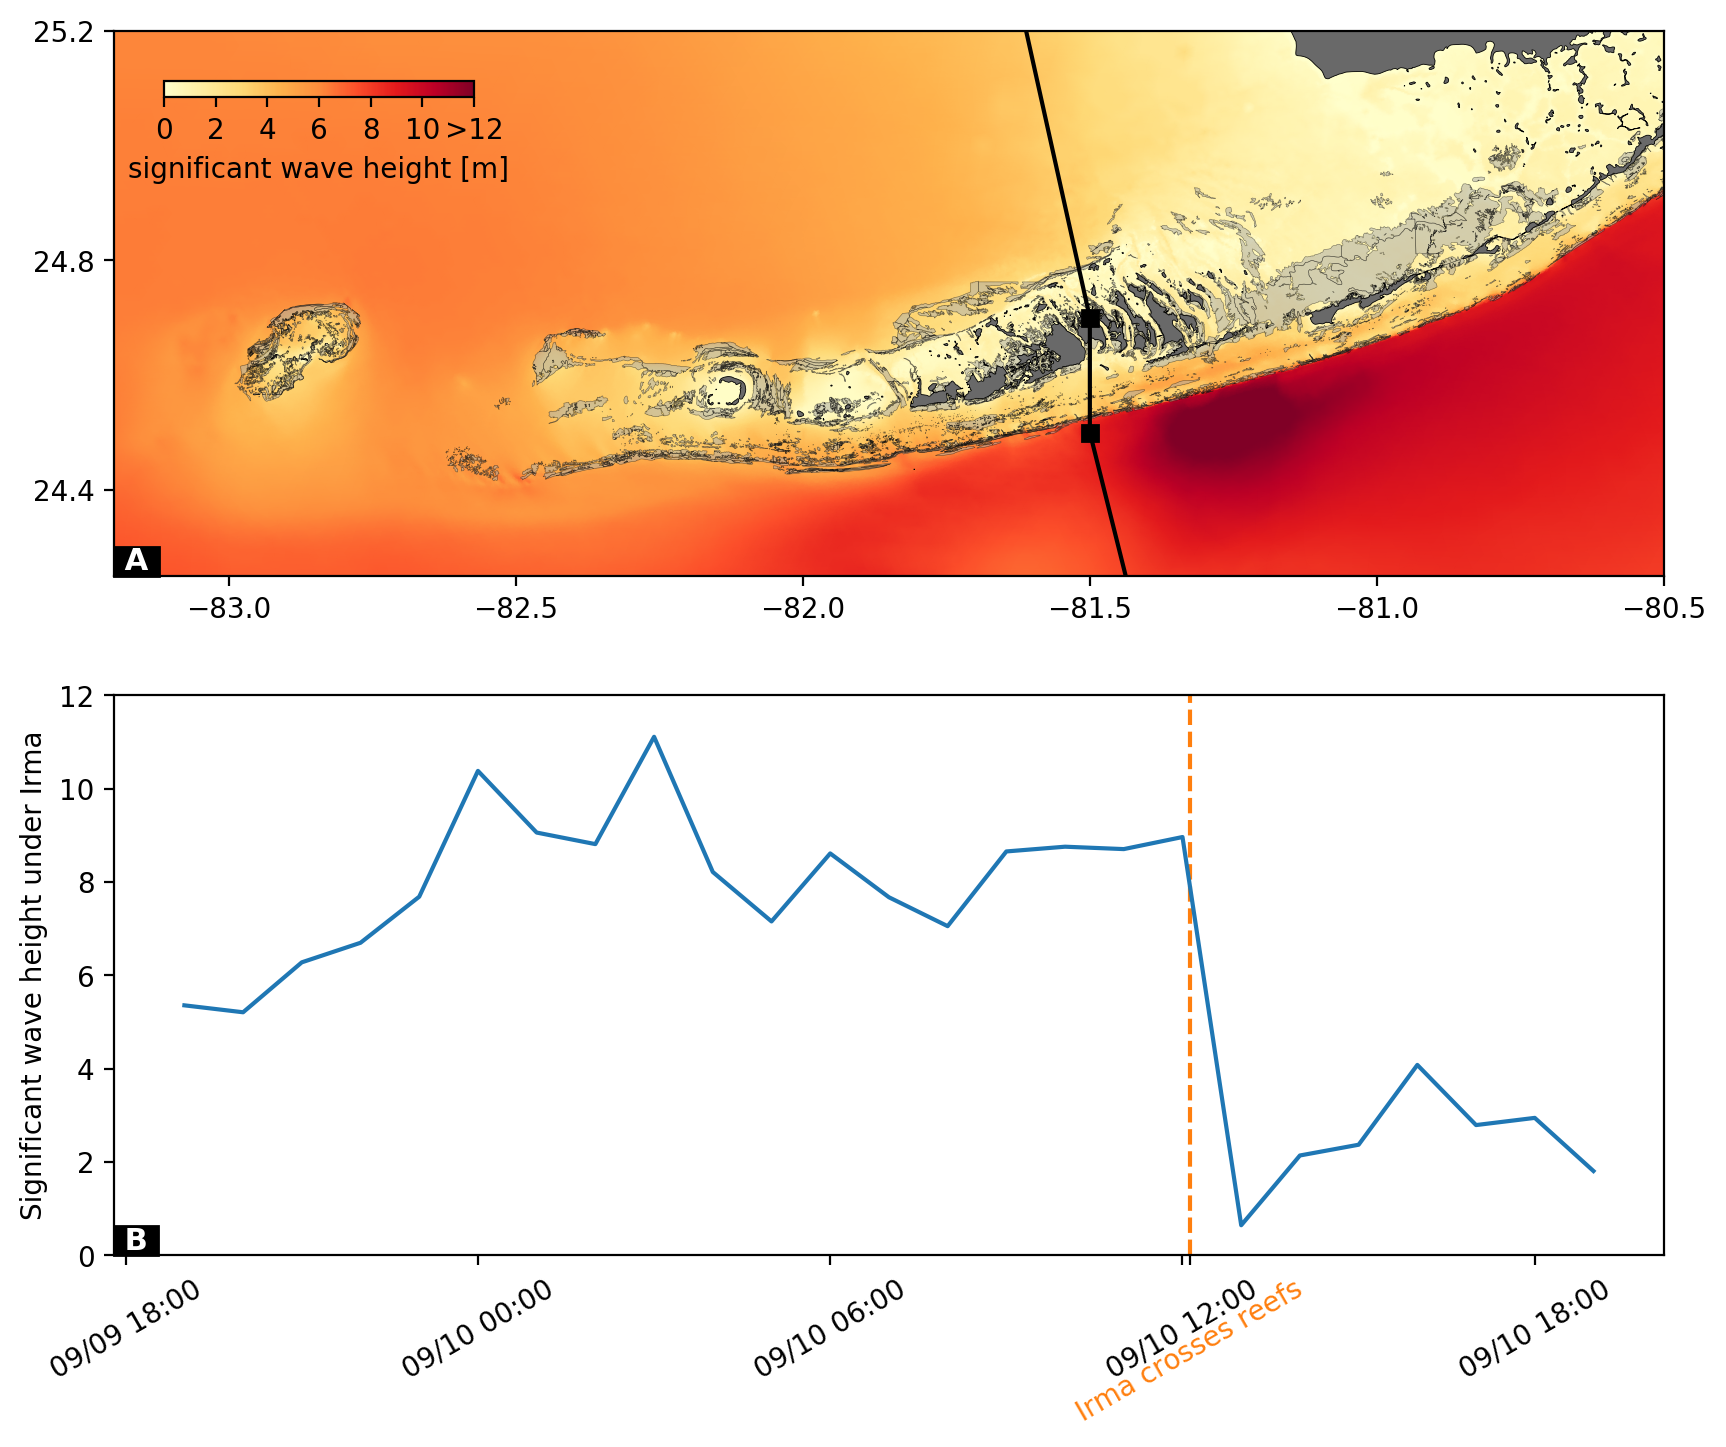
\includegraphics[width=\textwidth]{chapters/conclusions/figures/swh_curve.png}
    \caption{\textbf{A}: Snapshot of the significant wave height modeled by the coupled SLIM+SWAN model during Hurricane Irma, on Sept 10, 2017 at 1200 UTC. The path of the hurricane is shown by a black line with squares. Land is shown in dark gray and reefs in light gray. \textbf{B}: Evolution of the significant wave height under the center of Irma. Important wave attenuation is visible between the fringing coral reefs and the islands.}
    \label{ccl:swh}
\end{figure}

% Last nice chapter
The work presented in this thesis has demonstrated the capabilities of modeling tools to inform the management of Florida's Coral Reef. Models allow the evaluation of hypotheses derived from field observations on large-scale systems and can help infer the characteristics and underlying mechanisms of complex processes. Furthermore, they can be used in a predictive manner to evaluate the impacts of changing environmental conditions on a given ecosystem. Additionally, the framework developed in this thesis relies on the same widely used tools as larval transport models. Both approaches could thus be easily combined to optimize the design of coral reef protection and restoration campaigns. The development of such modeling tools coupled with field an lab studies may thus inform reef management to maintain the biological functions of coral reefs through the Anthropocene.    
%%
%
  \clearemptydoublepage
  \bibliography{include/bibliography.bib}

\end{document}